\batchmode
\makeatletter
\def\input@path{{style/}{sections/}}
\makeatother
\documentclass[letterpaper,spanish,svgnames,x11names,x11names,HTML]{report}
\usepackage{enumitem}%%% enumerar
\usepackage{refcount}
\usepackage{marco}
\usepackage{multicol}
\usepackage{pdfpages}
%\usepackage{kpfonts}
%\usepackage{eso-pic} 
\usepackage{cite}%para agrupar citas
%\usepackage{geometry}
\usepackage[paperheight=27.9cm,%
paperwidth=20.6cm,%
%centering,%
textheight=25.9cm,
left=2.5cm,%
right=2.5cm,%
top=5cm,%
bottom=-5cm,%
headheight=1cm,%
headsep=20pt,%
footskip=1cm,%
marginparsep=20pt,%
pdftex=false,%
letterpaper%
]{geometry}
%\usepackage{xcolor}
\usepackage[some]{background}
%\usepackage{lipsum}
\usepackage{chapterbib}
%%%%%%%%%%%%%%%

\usepackage{lettrine}
%\usepackage{keyval}% http://ctan.org/pkg/keyval
%\usepackage{environ}% http://ctan.org/pkg/environ
\usetikzlibrary{calc,trees,positioning,arrows,chains,shapes.geometric,
decorations.pathreplacing,decorations.pathmorphing,shapes,%
matrix,shapes.symbols,plotmarks,decorations.markings,shadows}
%\usepackage{theoremref} %refereciar teoremas Por ejemplo: \thlabel{foobar}
\usepackage{numprint}
\usepackage{mathtools,amsmath}
\usepackage{refstyle}
\usepackage{marginnote}
\usepackage{fancybox}
\usepackage{hhline}
\usepackage{multirow} 
\usepackage{colortbl}%
\usepackage{pifont} 
\usepackage{eurosym} %para el Euro
%\usepackage{xltxtra}%para logos de la familia TeX
%\usepackage{mathspec}
\usepackage{metalogo}
\usepackage{afterpage}% for "\afterpage"
\usepackage{lipsum-es}
%\usepackage{xparse}% para declarar comandos
\usepackage{amssymb}
%\usepackage[thref,thmmarks,framed, amsthm]{ntheorem}
\usepackage{comment}
\usepackage[explicit]{titlesec}
\usepackage{emptypage}%pagina en blanco al final de capitulo
%%%%%%%%%%%%%%%%%%%%%%%%%%%%%%
%\documentclass[openany,svgnames,x11names]{book}
\usepackage{titletoc}
\usepackage{fancyhdr}
\usepackage{pagecolor}
\usepackage[spanish]{layout}
%\usepackage{ucs}%codificacion vieja
\usepackage[utf8x,latin1]{inputenc}
%\usepackage[latin1]{inputenc}
%\usepackage{showframe}% traza layout en cada pagina
%%%======================================revisar
\usepackage{pifont}
\usetikzlibrary{shapes,snakes,positioning}
\pgfdeclarelayer{background}
\pgfdeclarelayer{foreground}
\pgfsetlayers{background,main,foreground}
\usepackage{wallpaper}
\usetikzlibrary{calc}
\usetikzlibrary{arrows}
\usepackage{epstopdf}
\usepackage{floatflt}
\usepackage{pgfplots}
\usepackage{setspace}
\usepackage{float}
%\usepackage{booktabs}
\usepackage{courier}
\usepackage{units}
\usepackage{url}
\usepackage{float}
\usepackage{mathpazo}
%\usepackage{amsfonts}
\usepackage{amsthm}
\usepackage{fancyvrb}
\usepackage{enumerate}
\usepackage{ifthen}
\usepackage{cancel}
\usepackage{layout}
\usepackage{footnote}
\usepackage{etex}%si pgfplot tiene problemas con new dim
\usepackage[frame,letter,cam]{crop}
\usepackage{microtype,soul,filecontents}
\usepackage{bbding}
\usepackage{lettrine,caption,multicol}
\usepackage{soul}
\usepackage{palatino}
\usepackage{calligra}
\usepackage[T1]{fontenc}
\usepackage[listings]{tcolorbox}
\tcbuselibrary{skins}
\usepackage{filecontents,ragged2e}
\usepackage{floatflt}
\usepackage[makeindex]{imakeidx}
\usepackage{chapterbib}   
\usepackage{lmodern}
\usepackage{etoolbox}
\usepackage{tabularx}
% \usepackage{flushend} % balance de las columnas con twocolumn
%\usepackage{minitoc}
\usepackage{etoc}
\usepackage{listings}
\definecolor{lightgrey}{rgb}{0.9,0.9,0.9}
\definecolor{darkgreen}{rgb}{0,0.6,0}
\usepackage{fourier-orns}
% % % % % % % % % % % % % % % % % % % % % % % % % % %
% % % %preamble de framed % % %
\usepackage{fixltx2e}
%\usepackage{etex}
\usepackage{textcomp}
\usepackage{array}
\usepackage{booktabs}
\usepackage{microtype}
\graphicspath{{ps/}{logo/}{image/}{pdf/}}
%%%%%%%%%%%%%%%%%%%%%%%%%%%%%%%%%%%%%%%%%%%%%%%%%%%%%%%%%%%%
\newcommand*{\mail}[1]{\href{mailto:#1}{\texttt{#1}}}
\newcommand*{\pkg}[1]{\textsf{#1}}
\newcommand*{\cs}[1]{\texttt{\textbackslash#1}}
\makeatletter
\newcommand*{\cmd}[1]{\cs{\expandafter\@gobble\string#1}}
\makeatother
\newcommand*{\env}[1]{\texttt{#1}}
\newcommand*{\opt}[1]{\texttt{#1}}
\newcommand*{\meta}[1]{\textlangle\textsl{#1}\textrangle}
\newcommand*{\marg}[1]{\texttt{\{}\meta{#1}\texttt{\}}}
%%%%%%%%%%%%%%%%%%%%%%%%%%%%%%%%% definicion de colores ================)
\definecolor{est1}{RGB}{0,177,235}
\definecolor{est2}{RGB}{0,119,158}
\definecolor{est3}{RGB}{235,137,0}
\definecolor{est4}{RGB}{158,66,0}
\definecolor{est5}{RGB}{20,20,20}
\definecolor{est6}{RGB}{235,235,235}
\definecolor{naranja1}{rgb}{1,0.5,0}
\definecolor{naranja2}{RGB}{255,127,0}
\definecolor{naranja3}{cmyk}{0,0.5,1,0}
\definecolor{naranja4}{HTML}{FF7F00}
\definecolor{WHITE}{HTML}{FF7F00}
%rgb
\definecolor{rojo}{rgb}{1,0,0}
\definecolor{verde}{rgb}{0,1,0}
\definecolor{azul}{rgb}{0,0,1}
%cmyk
\definecolor{blanco}{cmyk}{0,0,0,0}
\definecolor{cian}{cmyk}{1,0,0,0}
\definecolor{magenta}{cmyk}{0,1,0,0}
\definecolor{amarillo}{cmyk}{0,0,1,0}
\definecolor{negro}{cmyk}{0,0,0,1}
\definecolor{theblue}{rgb}{0.02,0.04,0.48}
\definecolor{thered}{rgb}{0.65,0.04,0.07}
\definecolor{thegreen}{rgb}{0.06,0.44,0.08}
\definecolor{thegrey}{gray}{0.5}
\definecolor{theshade}{gray}{0.94}
\definecolor{theframe}{gray}{0.75}
\definecolor{burl}{rgb}{0.27,0.22,0.20}
\definecolor{caper}{rgb}{0.36,0.46,0.23}
\definecolor{rhodo}{rgb}{0.58,0.63,0.45}
\definecolor{wood}{rgb}{0.61,0.51,0.43}
\definecolor{mesh}{rgb}{0.97,0.93,0.81}
\definecolor{wood}{rgb}{0.61,0.51,0.43}
\definecolor{doc}{RGB}{0,60,110}
\definecolor{boxheadcol}{gray}{.6}
\definecolor{boxcol}{gray}{.9}
\definecolor[named]{PowderBlue}{HTML}{B0E0E6}
\definecolor[named]{MidnightBlue}{HTML}{191970}
\definecolor{bl}{rgb}{0,0.2,0.8}
\definecolor{shcolor}{HTML}{FDEDD0}
\definecolor[named]{GreenTea}{HTML}{CAE8A2}
\definecolor[named]{MilkTea}{HTML}{C5A16F}
\definecolor[named]{SaddleBrown}{HTML}{8B4513}
\definecolor{FrameColor}{rgb}{0.25,0.25,1.0}
\definecolor{TitleColor}{rgb}{1.0,1.0,1.0}
\definecolor{TFFrameColor}{HTML}{CAE8A2}
\definecolor{TFTitleColor}{HTML}{C5A16F}
\definecolor{secnum}{RGB}{13,151,225}
\definecolor{ptcbackground}{RGB}{179,198,207}
\definecolor{ptctitle}{RGB}{3,76,117}
\definecolor{shadecolor}{RGB}{212,237,252}
\definecolor{visgreen}{rgb}{0.733, 0.776, 0}
\definecolor{myBGcolor}{HTML}{F6F0D6}
\definecolor[named]{PowderBlue}{HTML}{B0E0E6}
\definecolor[named]{MidnightBlue}{HTML}{191970}
\definecolor{mybrown}{RGB}{128,64,0}
\definecolor{lightgrey}{rgb}{0.9,0.9,0.9}
\definecolor{darkgreen}{rgb}{0,0.6,0}
\definecolor{Tan}{cmyk}{0.14,0.42,0.56,0}
%%%%%%%%%%%% lista%%%%%%%
\makeatletter
\newcommand\statuslabel[3][]{%
    \def\scale{#1}
    \ifx\scale\empty\def\scale{1}\fi
 
    \let\no\relax
    \let\n\relax
    \newcommand \no {#2}
    \newcommand \n {#3}
    \def \colorbef {blue}
    \def \colorat {orange}
    \def \coloraft {black!40}
 
    \let\stop\relax
    \sbox\z@{\@tempcnta=0\no\relax}\ifdim\wd0>\z@\relax\@latex@warning{Not a number (\#2): \no}\def\stop{1}\fi
    \sbox\z@{\@tempcnta=0\n\relax}\ifdim\wd0>\z@\relax\@latex@warning{Not a number (\#3): \n}\def\stop{1}\fi
    \ifx\stop\relax
        \ifnum\no>\n\@latex@warning{Wrong parameter order?}\def\stop{1}\fi
    \fi
 
    \ifx\stop\relax
    \else
        \def \no {1}
        \def \n {1}
        \def \colorat {red}
        \def \stop {??}
    \fi
 
    \begin{tikzpicture}[scale=0.1*\scale]
 
    \def \radiusout {2cm}
    \def \radiusin {1.3cm}
    \ifnum\n=1
        \def \margin {0}
    \else
        \def \margin {25/\n}
    \fi
 
    \foreach \s in {1,...,\n}
    {
        \node[circle, scale=\scale] at (0,0) {\tiny\stop};
        \fill[\ifnum\s>\no\coloraft\relax\else\ifnum\s<\no\colorbef\else\colorat\fi\fi]
            ({90-360/\n * (\s - 1)-\margin}:\radiusout) arc ({90-360/\n * (\s - 1)-\margin}:{90-360/\n * (\s)+\margin}:\radiusout) --
            ({90-360/\n * (\s)+\margin}:\radiusin) arc ({90-360/\n * (\s)+\margin}:{90-360/\n * (\s - 1)-\margin}:\radiusin);
    }
    \end{tikzpicture}
}
 \newcounter{myenum} % to create unique labels
\newenvironment{myenum}
  {\stepcounter{myenum}
   \edef\nref{\getrefnumber{myenum@\arabic{myenum}}}
   \edef\nref{\expandafter\@firstofone\nref}
   \begin{enumerate}[
     label=\protect\statuslabel{\arabic*}{\nref},
     ref=\arabic*]}
  {\label{myenum@\arabic{myenum}}%
   \end{enumerate}}
\makeatother

%%%%%%%%%%%%%%%%%
%%%%%%%%%%%%%%%%
%%%%% Definicion de listing===========
\usepackage{caption}
\DeclareCaptionFont{white}{\color{white}}
\DeclareCaptionFormat{listing}{\colorbox{gray}{\parbox{\dimexpr\textwidth-2\fboxsep\relax}{C\'odigo \thesection .\ 
\thesource\ #3}}}
\captionsetup[source]{format=listing,labelfont=white,textfont=white, singlelinecheck=false, margin=0pt, font={bf,footnotesize}}
\newcounter{source}[section]
\lstnewenvironment{source}[2][]
{\refstepcounter{source}
\captionsetup{options=source}
\lstset{%
basicstyle=\tiny\ttfamily\bf,language={[LaTeX]TeX},caption=#1,label=#2,  
numbersep=5mm, numbers=left, numberstyle=\tiny, % number style
breaklines=true,framexleftmargin=10mm, xleftmargin=10mm,
backgroundcolor=\color{ptcbackground!60},frameround=fttt,escapeinside=??,
rulecolor=\color{ptctitle},
morekeywords={% Give key words here                                         % keywords
    maketitle},
keywordstyle=\color[rgb]{0,0,1},                    % keywords
        commentstyle=\color[rgb]{0.133,0.545,0.133},    % comments
        stringstyle=\color[rgb]{0.627,0.126,0.941}  % strings
%columns=fullflexible   
}
        }
{}
%%%%%%%%%%secciones
\makeatother
\usepackage{fancyvrb}
\usepackage{cancel}
\usepackage[unicode=true,pdfusetitle,
 bookmarks=true,bookmarksnumbered=true,bookmarksopen=true,bookmarksopenlevel=1,
 breaklinks=false,pdfborder={0 0 0},backref=false,colorlinks=false]
 {hyperref}
\hypersetup{
 pdfpagelayout=OneColumn, pdfnewwindow=true, pdfstartview=XYZ, plainpages=false}

%%%%%%%%%%%%%%%%%
\preto{\frontmatter}{\pagecolor{ptcbackground}}{}{}
\preto{\mainmatter}{\pagecolor{white}}{}{}
\preto{\backmatter}{\pagestyle{empty}\pagecolor{myBGcolor}}{}{}{}
%%%%%%%%%%%%Definicionn de cap\'itulo%%%%%%%%%%%%%
\newcommand*\chapterlabel{}
\titleformat{\chapter}
  {\gdef\chapterlabel{}
     \normalfont\sffamily\huge\bfseries\scshape}
  {\gdef\chapterlabel{\thechapter\ }}{0pt}
  {\begin{tikzpicture}[remember picture,overlay]
    \node[yshift=-3cm] at (current page.north west)
      {\begin{tikzpicture}[remember picture, overlay]
        \draw[fill=ptcbackground!60,draw=ptcbackground!60] (0,0) rectangle
          (\paperwidth,3cm);
          \draw[ultra thick,fill=ptctitle,draw=ptctitle](0,0) -- (current page.east |- 0,0 );
          \draw [ptctitle,fill=ptctitle, ultra thick] (0.5,0) circle [radius=0.1];
         \draw[ptctitle,fill=ptctitle, ultra thick] (21,0) circle [radius=0.1];
        \node[anchor=east,xshift=.9\paperwidth,rectangle,
              rounded corners=20pt,inner sep=11pt,
              fill=ptctitle,draw=ptctitle]
              {\color{white} \chapterlabel\protect#1};
%               \draw[fill=green] (current page.north west) rectangle (current page.south east);
       \end{tikzpicture}        
      }; 
      \begin{pgfonlayer}{background}
%          \path (-1.4cm,2.8cm) node (tl) {};
%          \path (2.3cm, -8.4cm) node (br) {};
          \path (current page.north west) rectangle (current page.south east);
      \end{pgfonlayer}
   \end{tikzpicture}  
     \vspace{20pt}
  }
\titlespacing*{\chapter}{0pt}{50pt}{-60pt}

%%%======================================== TOC
    %%%%%%%%%%%%%%%%%%%%%%%%%%%%%%%%%%
%    \renewcommand{\theequation}{\thesection.\arabic{equation}}
%\renewcommand{\thesection}{\arabic{section}}
%\renewcommand{\thesubsection}{(\alph{subsection})}

 \setcounter{tocdepth}{0}
    \titlecontents{subsection}
  [5.8em]{\scriptsize\sffamily}
  {\color{ptctitle}\contentslabel{5.5em}\normalcolor}{}
  {\titlerule*[1000pc]{.}\contentspage\hspace*{-5.8em}\\\hspace*{-5.8em}\vspace*{2pt}%
    \color{ptctitle}\rule{\dimexpr\textwidth-15.5pt\relax}{1pt}}

    %%%%%%%%%%%%%%%%%%%%%%%%%%%%%%%
    \titlecontents{section}
  [5.8em]{\color{ptctitle}\scriptsize\sffamily}
  {\color{ptctitle}\contentslabel{5.5em}\normalcolor}{}
  {\titlerule*[1000pc]{.}\contentspage\hspace*{-2em}\\\hspace*{-3em}\vspace*{2pt}%
    \color{ptctitle}\rule{\dimexpr\textwidth-20pt\relax}{1pt}}

\titlecontents{lsection}
  [5.8em]{\color{white}\sffamily}
  {\color{ptctitle}\contentslabel{3.5em}\normalcolor}{}
  {\titlerule*[1000pc]{.}\contentspage\\\hspace*{-5.8em}\vspace*{2pt}%
    \color{ptctitle}\rule{\dimexpr\textwidth-15.5pt\relax}{1pt}}

\makeatletter
\renewcommand*\l@chapter[2]{%
\thispagestyle{empty}
\pagecolor{ptcbackground}
  \ifnum \c@tocdepth >\m@ne
    \addpenalty{-\@highpenalty}%
    \vskip 1.0em \@plus\p@
    \setlength\@tempdima{1.5em}%
    \begingroup
      \parindent \z@ \rightskip \@pnumwidth
      \parfillskip -\@pnumwidth
      \leavevmode
      \advance\leftskip\@tempdima
      \hskip -\leftskip
      \colorbox{ptctitle}{\strut%
        \makebox[\dimexpr\textwidth-2\fboxsep-7pt\relax][l]{%
          \color{white}\bfseries\sffamily\protect#1%
          \nobreak\hfill\nobreak\hb@xt@\@pnumwidth{\hss #2}}}\par\smallskip
                \penalty\@highpenalty
    \endgroup
  \fi}
\makeatother
%%% crear toc por capitulo con etoc
\renewcommand*\contentsname{Contenido} 
\newcommand*\chaptertoc{% 
  \setcounter{tocdepth}{2}% 
  \etocsettocstyle{\subsection*{\subtoc}}{}% 
  { \footnotesize\localtableofcontents }
} 
\def\subtoc{\colorbox{ptctitle}{
\renewcommand{\baselinestretch}{1}
     \parbox[t]{\dimexpr\textwidth-2\fboxsep\relax}{%
    \strut\color{white}\bfseries\sffamily \makebox[7em]{%
Orden      }\hfill Eventos \hfill P\'agina}
}}
\AtBeginDocument{
  \addtocontents{toc}{\small}
  \addtocontents{lof}{\tiny}
}


%%%%%%%%

%%%%%%%%
\def\etocstandarddisplaystyle{\etocarticlestyle}
%%%% crear toc por capitulo con titlesec
%\newcommand\PartialToC{%
%\startcontents[chapters]%
%\pagecolor{ptcbackground}
%\begin{mdframed}[backgroundcolor=ptcbackground,hidealllines=true]
%\printcontents[chapters]{l}{1}{\colorbox{ptctitle}{%
%  \parbox[t]{\dimexpr\textwidth-2\fboxsep\relax}{%
%    \strut\color{ptctitle}\bfseries\sffamily \makebox[5em]{%
%Contenido      }\hfill Cap\'{i}tulo~\thechapter\hfill P\'agina}}\vskip5pt}
%\end{mdframed}%
%}
% Define partial toc for part pages
%% Set the uniform width of the colour box
%% displaying the page number in footer
%% to the width of "99"
\newlength\pagenumwidth
\settowidth{\pagenumwidth}{99}

%% Define style of page number colour box
\tikzset{pagefooter/.style={
anchor=base,font=\sffamily\bfseries\small,
text=white,fill=ptctitle,text centered,
text depth=17mm,text width=\pagenumwidth}}

%% Concoct some colours of our own
\definecolor[named]{GreenTea}{HTML}{CAE8A2}
\definecolor[named]{MilkTea}{HTML}{C5A16F}
%%%%%%%%%%%%%%% Encabezado y pie de pagina
%%%%%%%%%%
%%% Re-define running headers on non-chapter pages
%%%%%%%%%%

\renewcommand{\chaptermark}[1]{ \markboth{#1}{}}
\fancypagestyle{headings}{%
  \fancyhf{}   % Clear all headers and footers first
  %% Right headers on odd pages
  \fancyhead[RO]{%
    %% First draw the background rectangles
    \begin{tikzpicture}[remember picture,overlay]
    \fill[ptcbackground] (current page.north east) rectangle (current page.south west);
    \fill[white, rounded corners] ([xshift=-10mm,yshift=-20mm]current page.north east) rectangle ([xshift=15mm,yshift=17mm]current page.south west);
    \begin{pgfonlayer}{background}
    %          \path (-1.4cm,2.8cm) node (tl) {};
    %          \path (2.3cm, -8.4cm) node (br) {};
              \path[fill=brown!20] (current page.north west) rectangle (current page.south east);
          \end{pgfonlayer}
    \end{tikzpicture}
    %% Then the decorative line and the right mark
    \begin{tikzpicture}[xshift=-.75\baselineskip,yshift=.25\baselineskip,remember picture,    overlay,fill=ptctitle,draw=ptctitle]\fill circle(3pt);
    \draw[semithick](0,0) -- (current page.west |- 0,0);
        \end{tikzpicture} \sffamily\itshape\small\protect\nouppercase{Vig\'esima Octava Reuni\'on Latinoamericana de Matem\'aticas Educativa}
  }

  %% Left headers on even pages
  \fancyhead[LE]{%
    %% Background rectangles first
    \begin{tikzpicture}[remember picture,overlay]
     \fill[brown!20] (current page.north east) rectangle (current page.south west);
    \fill[ptcbackground] (current page.north east) rectangle (current page.south west);
    \fill[white, rounded corners] ([xshift=-15mm,yshift=-20mm]current page.north east) rectangle ([xshift=10mm,yshift=17mm]current page.south west);
           \end{tikzpicture}
    %% Then the right mark and the decorative line
    \sffamily\itshape\small\protect\nouppercase{Vig\'esima Octava Reuni\'on Latinoamericana de Matem\'aticas Educativa}\ 
    \begin{tikzpicture}[xshift=.5\baselineskip,yshift=.25\baselineskip,remember picture, overlay,fill=ptctitle,draw=ptctitle]
    \fill (0,0) circle (3pt); \draw[semithick](0,0) -- (current page.east |- 0,0 );
       \end{tikzpicture}
  }

  %% Right footers on odd pages and left footers on even pages,
  %% display the page number in a colour box
  \fancyfoot[RO,LE]{\tikz[baseline]\node[pagefooter]{\thepage};}
   \fancyfoot[CO,CE]{\tikz\node{\color{ptctitle}Barranquilla - Colombia};}
  \renewcommand{\headrulewidth}{0pt}
  \renewcommand{\footrulewidth}{0pt}
}

%%%%%%%%%%
%%% Re-define running headers on chapter pages
%%%%%%%%%%
\fancypagestyle{plain}{%
  %% Clear all headers and footers
  \fancyhf{}
  %% Right footers on odd pages and left footers on even pages,
  %% display the page number in a colour box
  \fancyfoot[RO,LE]{\tikz[baseline]\node[pagefooter]{\thepage};}
 
  
    %% First draw the background rectangles
     \fancyhead[LE]{\begin{tikzpicture}[remember picture,overlay]
    \fill[ptcbackground] (current page.north east) rectangle (current page.south west);
    \fill[white, rounded corners] ([xshift=-10mm,yshift=-20mm]current page.north east) rectangle ([xshift=15mm,yshift=17mm]current page.south west);
    \begin{pgfonlayer}{background}
    %          \path (-1.4cm,2.8cm) node (tl) {};
    %          \path (2.3cm, -8.4cm) node (br) {};
              \path[fill=ptcbackground] (current page.north west) rectangle (current page.south east);
          \end{pgfonlayer}
    \end{tikzpicture}
    \sffamily\itshape\small\protect\nouppercase{\rightmark}
  }
    \fancyhead[RO]{%
    %% First draw the background rectangles
    \begin{tikzpicture}[remember picture,overlay]
    \fill[ptcbackground] (current page.north east) rectangle (current page.south west);
    \fill[white, rounded corners] ([xshift=-10mm,yshift=-20mm]current page.north east) rectangle ([xshift=15mm,yshift=17mm]current page.south west);
    \begin{pgfonlayer}{background}
    %          \path (-1.4cm,2.8cm) node (tl) {};
    %          \path (2.3cm, -8.4cm) node (br) {};
              \path[fill=ptcbackground] (current page.north west) rectangle (current page.south east);
          \end{pgfonlayer}
    \end{tikzpicture}
    \sffamily\itshape\small\protect\nouppercase{\rightmark}
  }
  \renewcommand{\headrulewidth}{0pt}
  \renewcommand{\footrulewidth}{0pt}
}
\fancypagestyle{eimat}{
 %% Clear all headers and footers
  \fancyhf{}
  %% Right footers on odd pages and left footers on even pages,
  %% display the page number in a colour box
  \fancyfoot[RO,LE]{\tikz[baseline]\node[pagefooter]{\thepage};}
   \fancyhead[LE]{
   %% Then the right mark and the decorative line
    \sffamily\itshape\small\protect\nouppercase{\color{ptctitle}\footnotesize XII ENCUENTRO INTERNACIONAL DE MATEM\'ATICAS - EIMAT}} 
    
   \fancyhead[RO]{
    \sffamily\itshape\small\protect\nouppercase{\color{ptctitle}\footnotesize XII ENCUENTRO INTERNACIONAL DE MATEM\'ATICAS - EIMAT } 
    }
       \fancyfoot[CO,CE]{\tikz\node{\color{ptctitle}\footnotesize\leftmark};}
   \renewcommand{\headrulewidth}{0pt}
  \renewcommand{\footrulewidth}{0pt}
 }
 \fancypagestyle{empty}{
  \renewcommand{\headrulewidth}{0pt}
  \renewcommand{\footrulewidth}{0pt}
 \pagecolor{ptcbackground}
  \fancyhf{}
 \fancyhead{}
 \fancyfoot{}}
 
%%%%%%%%%%%%%%%%%%%%%%%%%%%%%%% empty page

%%%%%% def de seccion

\newcommand\titlebar{%
\tikz[baseline,trim left=0cm,trim right=3cm] {
    \node [
        fill=white!90!ptcbackground,
        text = ptctitle,
        anchor= base east,
        minimum height=5.5ex] (a) at (3cm,0.2cm) {
        \textbf{\thesection}
    };
}%
}
\titleformat{\section}{\filcenter\normalfont\footnotesize\sf}{\titlebar}{0.25cm}{\textcolor{white}{#1}}      %% Change color if needed and remove \sf.
\titlespacing*{\section}{-2cm}{3.5ex plus 1ex minus .2ex}{2.3ex plus .2ex}
\renewcommand*{\thesection}{\arabic{section}}
%%%%%%%%%%%%%%%

%%%%%%%%%%%%%%%%%%%%%%%%%%%%%%%%%%%%%%%
\makeatletter
\renewenvironment{thebibliography}[1]
    {{\hspace*{5pt}\color{ptctitle}\Large Referencias}% <-- this line was changed from \chapter* to \section*
      %\@mkboth{\MakeUppercase\Referencias}{\MakeUppercase Referencias}%
      \small
      \list{\@biblabel{\@arabic\c@enumiv}}%
           {\settowidth\labelwidth{\@biblabel{#1}}%
            \leftmargin\labelwidth
            \advance\leftmargin\labelsep
            \@openbib@code
            \usecounter{enumiv}%
            \let\p@enumiv\@empty
            \renewcommand\theenumiv{\@arabic\c@enumiv}}%
      \sloppy
      \clubpenalty4000
      \@clubpenalty \clubpenalty
      \widowpenalty4000%
      \sfcode`\.\@m}
     {\def\@noitemerr
       {\@latex@warning{Empty `thebibliography' environment}}%
      \endlist}
      %%%%%%%%%%%%%%%%%5empieza title%%%%%%%%%5
     \providecommand{\keywords}[1]{\textbf{\textit{Keywords:}} #1}
     \providecommand{\palabras}[1]{\textbf{\textit{Palabras Claves:}} #1}
  


%%%%%%%%%%%%%%%%%%%%%%%%%%%%%%%%
%%%%%%%%%%%%%%%resumen
\makeatletter
\if@titlepage
  \newenvironment{resumen}{%
      \titlepage
      \null\vfil
      \@beginparpenalty\@lowpenalty
      \begin{center}%
        \bfseries Resumen
        \@endparpenalty\@M
      \end{center}}%
     {\par\vfil\null\endtitlepage}
\else
  \newenvironment{resumen}{%
      \if@twocolumn
        \section*{\abstractname}%
      \else
                \begin{center}%
          {\bfseries Resumen\vspace{-.5em}\vspace{\z@}}%
        \end{center}%
        \quotation
      \fi}
      {\if@twocolumn\else\endquotation\fi}
      \fi
      %%%%%%%%%
      \if@titlepage
  \renewenvironment{abstract}{%
      \titlepage
      \null\vfil
      \@beginparpenalty\@lowpenalty
      \begin{center}%
        \bfseries Abstract
        \@endparpenalty\@M
      \end{center}}%
     {\par\vfil\null\endtitlepage}
\else
  \renewenvironment{abstract}{%
      \if@twocolumn
        \section*{\abstractname}%
      \else
                \begin{center}%
          {\bfseries Abstract\vspace{-.5em}\vspace{\z@}}%
        \end{center}%
        \quotation
      \fi}
      {\if@twocolumn\else\endquotation\fi}
      \fi
      
\makeatother
%%%%%%%%%%%%%%%%
\def\tema#1{\'Area:\ #1}
\def\thanks#1{\footnote{Thanks:\ #1}}
\def\gracias#1{\footnote{Agradecimientos:\ #1}}
\definecolor{titlepagecolor}{cmyk}{1,.60,0,.40}

\DeclareFixedFont{\bigsf}{T1}{phv}{b}{n}{0.5cm}

\backgroundsetup{
scale=1,
angle=0,
opacity=1,
contents={\begin{tikzpicture}[remember picture,overlay]
 \path [fill=ptctitle] (-0.5\paperwidth,9) rectangle (0.5\paperwidth,12.5);  
\end{tikzpicture}}
}
\makeatletter                       
\def\printauthor{%                  
    {\small \bf\@author}}              
\makeatother
\author{%
\tema{Tema}\\
    Author 1 name \\
    Department name \\
    \texttt{email1@example.com}\vspace{40pt} \\
    Author 2 name \\
    Department name \\
    \texttt{email2@example.com}\\
         }
        
         %%%%%%%%%%%%
         %%%%%%%%%%%%%%
         \makeatletter % copy and edit the original code - this is from article.cls, the others may be slightly different. 
         \if@compatibility
          \renewenvironment{titlepage} % changed from "newenvironment" 
         {%
         \stepcounter{page} 
         \if@twocolumn \@restonecoltrue\onecolumn \else \@restonecolfalse\newpage \fi \thispagestyle{eimat}% Changed from "empty" 
         %\setcounter{page}\z@ 
         }% 
         {\if@restonecol\twocolumn \else \newpage \fi } \else \renewenvironment{titlepage} % changed from "newenvironment"
          {% 
          \if@twocolumn \@restonecoltrue\onecolumn \else \@restonecolfalse\newpage \fi \thispagestyle{eimat}% changed from "empty" 
          %\setcounter{page}\@ne 
          }% 
          {\if@restonecol\twocolumn \else \newpage \fi \if@twoside\else %\setcounter{page}\@ne 
          \fi } \fi % End of copied code \makeatother


         %%%%%%%%%%%%%%%%%%%%%%%%%%%%
         \newtheorem{thm}{Teorema}[section]
%\newtheorem{cor}[thm]{Definici\'on}
\newtheorem{prop}{Proposici\'{o}n}[section]
\DeclareMathOperator{\ess}{ess}
%%%%%%%%%%%%%%%%%%%%%%%%%%%%%%%%%%%%%%%%%%%%%%%%%%%
%%%%%%%%%%% definicion del cover
%\tcbset{
%    pccstyle/.style={
%        enhanced,flushright upper,
%        boxrule=1.4pt,
%        colback=white,colframe=black!50!yellow,
%        drop fuzzy midday shadow=black!50!yellow
%    }
%}
%
%\AddToShipoutPicture{% from package eso-pic: put something to the background
%    \AtPageCenter{% start the bar at the bottom right of the page
%        \put(-\LenToUnit{.465\paperwidth},-\LenToUnit{.4\paperheight}){% move it to the middle
%            %{\transparent{.5}{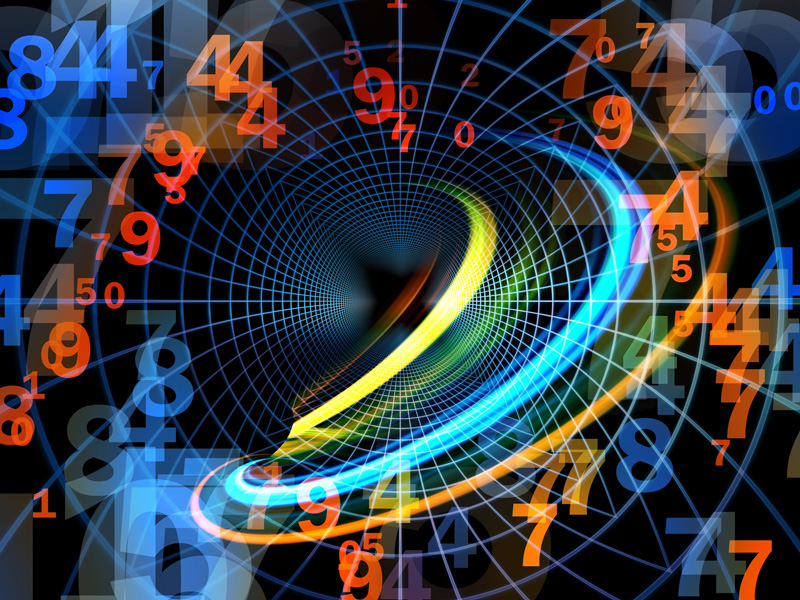
\includegraphics[width=20cm]{50th_mathematicsproof}}}
%            \begin{tcolorbox}[pccstyle,left=0mm,top=0mm,bottom=0mm]
%                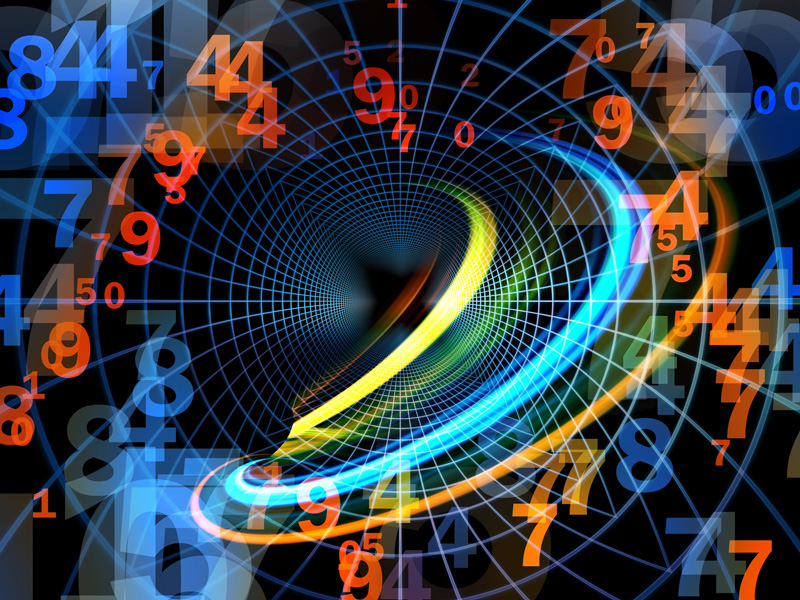
\includegraphics[width=20cm]{50th_mathematicsproof}
%            \end{tcolorbox}
%        }%
%    }%
%    \AtPageLowerLeft{% start the bar at the bottom right of the page
%        \put(\LenToUnit{\dimexpr\paperwidth-3cm},0){% move it to the top right
%            \color{blue}\rule{3cm}{\LenToUnit\paperheight}%
%        }%
%        \put(\LenToUnit{\dimexpr\paperwidth-2.7cm},\LenToUnit{17cm}){% move it to the top right
%            \color{gray}\scalebox{8}{$\sum$}
%        }%
%        \put(\LenToUnit{\dimexpr\paperwidth-2.5cm},\LenToUnit{12.5cm}){% move it to the top right
%            \color{gray}\scalebox{8}{$\int$}
%        }%
%        \put(\LenToUnit{\dimexpr\paperwidth-2.3cm},\LenToUnit{8.5cm}){% move it to the top right
%            \color{gray}\scalebox{8}{$e$}
%        }%
%        \put(\LenToUnit{\dimexpr\paperwidth-2.7cm},\LenToUnit{5.0cm}){% move it to the top right
%            \color{gray}\scalebox{8}{$\pi$}
%        }%
%        \put(\LenToUnit{\dimexpr\paperwidth-2.2cm},\LenToUnit{1.5cm}){% move it to the top right
%            \color{gray}\scalebox{8}{$i$}
%        }%
%    }%
%}

         %%%%%%%%%%%%%%%%%%%%%%%%%%%%%
         \newenvironment{lista}{
\begin{itemize}
 \renewcommand{\labelitemi}{{
 \colorbox{ptctitle}{\color{white}{\ding{42}}}
 }}
}{\end{itemize}}
         %%%%%%%%%%%%%%%%%%%%%%%%%
         %%%%%%%%%%%%%%%%%%%%%%%%%%%%%
         %%%%%%%%%%%%%%%%%%%%%%%%%%%%%%%%
         %%%%%%%%%%%%%%%%%%%%%%%%%%%%%%%%%
\begin{document}
\frontmatter
\pagestyle{empty}

\includepdf{cover2.pdf}
%%%%%%%%%%%%5cover
%\pagestyle{empty}
%
%\vspace*{1cm}
%\mbox{}\hfill\scalebox{2}{
%    \begin{tcolorbox}[pccstyle,width=7.8cm,left=5mm,top=0mm,bottom=0mm]
%    \centering
%        {\bfseries\LARGE {X ENCUENTRO INTERNACIONAL} \par}
%        {\bfseries\LARGE  DE MATEM\'ATICAS \\[10pt]}
%        {\large UNIVERSIDAD DEL ATL\'ANTICO }
%    \end{tcolorbox}
%}
%
%\vfill
%\centering
%
%\scalebox{2}{%
%    \begin{tcolorbox}[pccstyle,width=5cm,left=5mm,top=0mm,bottom=0mm]
%    \centering
%        {\tiny\scshape DEL 30 SEPTIEMBRE AL 6 OCTUBRE DE  2014\par}
%        {\tiny\scshape Barranquilla - Colombia}
%    \end{tcolorbox}
%}
%%%%%%%%%%%%pagina legal
%%%%%%%%%%%%%%%%%%%%%%%%%%%%%%%%%%%
%%%%%%%%%%%%%%%%%%%%%%%%%%%%%%%%
%%%%%%%%%%%%%%$$$$$$$$$$$$$$$$$$$$$$$$$$$$$$$
\newgeometry{textheight=25.9cm}
\pagestyle{empty}
\small
\pagecolor{ptcbackground}
%\pagecolor{white}
 \vfill
%\begin{multicols}{1}
%\onecolumn
{\color{black}
\bfseries \setlength\parindent{0pt}


\begin{mdframed}[backgroundcolor=ptctitle,hidealllines=true]
\parbox[t]{\dimexpr\textwidth-2\fboxsep\relax}{  \color{white}\bfseries\sffamily  \uppercase{Memoria Del Duod\'ecimo Encuentro Internacional de Matem\'aticas - EIMAT} }
\end{mdframed}\vspace{5pt}
EIMAT A\~no 2014\vspace{5pt}

Volumen 5 Nro. 1 A\~no 2016\vspace{5pt}

ISSN: 2346-1594\vspace{15pt}


\color{black}

\colorbox{ptctitle}{\color{white}\bfseries\sffamily EDITORES:}\\[5pt]

JORGE LUIS RODR\'IGUEZ CONTRERAS

ALEJANDRO URIELES GUERRERO

ALEJANDRO VILLAREAL DAZA

\vfill

 \begin{multicols}{2} 

\begin{figure}[H]
\centering
\includegraphics[scale=0.3]{antorcha}
\end{figure}
 
\begin{figure}[H]
\centering
\includegraphics[scale=0.3]{uac}
\end{figure}


 \end{multicols} 

\vfill

 \begin{multicols}{2} 

\colorbox{ptctitle}{\color{white}\bfseries\sffamily Rectora Universidad Del Atl\'antico :}\\[5pt]

ANA SOF\'IA MESA DE CUERVO

\colorbox{ptctitle}{\color{white}\bfseries\sffamily Rector Universidad Aut\'onoma Del Caribe :}\\[5pt]

\uppercase{ Ramses Vargas Lamadrid}

 \end{multicols} 

\vfill

\colorbox{ptctitle}{\color{white}\bfseries\sffamily VICERECTOR ADMINISTRATIVO Y FINANCIERO:}\\[5pt]

FREDDY D\'IAZ MENDOZA\vfill

\colorbox{ptctitle}{\color{white}\bfseries\sffamily VICERECTOR DE DOCENCIA:}\\[5pt]

REMBERTO DE LA HOZ REYES \vfill

\colorbox{ptctitle}{\color{white}\bfseries\sffamily VICERECTORA DE INVESTIGACI\'ON, EXTENSI\'ON Y PROYECCI\'ON SOCIAL:}\\[5pt]

RAFAELA VOS OBESO \vfill

\colorbox{ptctitle}{\color{white}\bfseries\sffamily DECANO FACULTAD DE CIENCIAS B\'ASICAS :}\\[5pt]

LUIS CARLOS GUTI\'ERREZ MORENO\vfill\vspace{3cm}

\textsf{El material de esta publicaci\'on no puede ser reproducido sin
la autorizaci\'on de los autores y editores. La responsabilidad del
contenido de este texto corresponde a sus autores.} \vfill

\begin{center}
\copyright UNIVERSIDAD DEL ATL\'ANTICO BARRANQUILLA - COLOMBIA 2014 
\par\end{center}

\begin{center}
\copyright UNIVERSIDAD AUT\'ONOMA DEL CARIBE BARRANQUILLA - COLOMBIA
2014
\par\end{center}


\vfill
\newpage
\newgeometry{left=2cm,right=2cm,top=2cm,bottom=2cm}
%%%%%%%%%%%%%%%%
%%%%%%%%%%%%%%%%%% Organizadores
\section*{\color{ptctitle}\Large Organizadores}
\small
\begin{mdframed}[backgroundcolor=ptctitle,hidealllines=true]
\parbox[t]{\dimexpr\textwidth-2\fboxsep\relax}{\color{white}\bfseries\sffamily  COMIT\'E CIENT\'IFICO }
\end{mdframed}
\begin{lista}
\item Dra. Yamilet Quintana, Universidad Sim\'on Bol\'ivar, Venezuela.\\
\item Dr. Alfonso Castro, Harvey Mudd College, Claremont-California, Estados Unidos.\\
\item Dr. Walter Beyer, Instituto Pedag\'ogico de Caracas-Universidad Pedag\'ogica Experimental Libertador, Venezuela.\\
\item Dr. Milton Rosa, Centro de Educa\c{c}\~ao Aberta e a Dist\^ancia, Universidade Federal de Ouro Preto, Brasil.\\
\item Dr. Carlos Carpintero, Universidad de Oriente, Venezuela.\\
\item Dr. Primitivo Acosta-Hum\'anez, Universidad del Atl\'antico \& INTELECTUAL.CO, Colombia.\\
\item Dr. Hugo Leiva, Universidad de los Andes, Venezuela.\\
\item Dr. Daniel Orey, Centro de Educa\c{c}\~ao Aberta e a Dist\^ancia, Universidade Federal de Ouro Preto, Brasil.\\
\end{lista}
%
%
\begin{mdframed}[backgroundcolor=ptctitle,hidealllines=true]
\parbox[t]{\dimexpr\textwidth-2\fboxsep\relax}{   \color{white}\bfseries\sffamily  COMIT\'E  ORGANIZADOR}
\end{mdframed}
\begin{lista}
\item  Presidente: Jorge Rodr\'iguez
\item Coordinador General: Alejandro Urieles
\item Coordinador locales: 
\begin{lista}
\item Jos\'e De la Hoz,
\item  Alejandro Villareal
\end{lista}
\end{lista}
%
\begin{mdframed}[backgroundcolor=ptctitle,hidealllines=true, rightmargin=0.5\textwidth]
\parbox[t]{\dimexpr\textwidth-2\fboxsep\relax}{  \color{white}\bfseries\sffamily  Miembros: }
\end{mdframed}
%
\begin{multicols}{2}
 \begin{lista} 
  \item Ang\'elica Arroyo
    \item Sonia Balbuena
    \item Claudia Baloco
   \item  John Beiro Moreno
    \item Alirio Gerardino
    \item Ant\'alcides Olivo
    \item Mar\'ia Jos\'e Ortega
    \item Ramiro Pe\~na
    \item Ennis Rosas
    \item Jorge Robinson
    \item Julio Romero
    \item Lesly Salas
    \item Diana Vargas
    \item Gabriel Vergara
   \item  Ludwing Villa
 \end{lista}
 \end{multicols} 
%
\newpage
%%%%%%%%%%%%%%%%%Presentaci\'on
\normalsize
\section*{\Large\color{ptctitle}      Presentaci\'on}
El Encuentro Internacional de Matem\'aticas EIMAT, es un evento acad\'emico que se ha realizado desde 2004, teniendo como sede la Universidad del Atl\'antico. El encuentro tiene un sentido amplio y est\'a dirigido a estudiantes, profesores e investigadores que trabajan en algnn campo de las matem\'aticas, bien sea dentro de la teor\'ia, la pr\'actica o la ense\~nanza.
 
Este evento organizado por el Programa de Matem\'aticas de la Universidad del Atl\'antico ha contado con la participaci\'on de profesores de reconocida trayectoria acad\'emica e investigativa a nivel nacional e internacional en diferentes \'areas de la matem\'atica y la educaci\'on matem\'atica.  

Los Objetivos del Encuentro Internacional de Matem\'aticas  son:
\begin{lista} 
\item Divulgar los trabajos matem\'aticos realizados por el grupo de investigadores nacionales e internacionales invitados.

\item Contribuir a la actualizaci\'on de matem\'aticos, f\'isicos, ingenieros y profesores de matem\'aticas tanto universitarios como de b\'asica y media.

\item Abrir espacios para el intercambio de ideas y conocimiento entre profesores universitarios y de educaci\'on b\'asica y  media.
\end{lista}
\newpage
%%%%%%%%%%%%%%%%%%
\let\myclearpage\clearpage
\tableofcontents{}
\let\myclearpage
\relax\newpage{}
\mainmatter
\color{black}
\chapter{An\'alisis y Topolog\'ia}
\chaptertoc
\thispagestyle{empty}
\pagecolor{ptcbackground}
\author{%
\tema{An\'alisis}\\
    Arturo Sanju\'an \\
    Universidad Distrital Francisco Jos\'e De Caldas \\
    \texttt{\footnotesize aasanjuanc@udistrital.edu.co}\vspace{40pt} \\
%    Author 2 name \\
%    Department name \\
%    \texttt{email2@example.com}\\
         }
\pagecolor{white}\afterpage{\nopagecolor}
\pagestyle{eimat}
\renewcommand\thesection{A\,$\&$T\ \nplpadding{2}\numprint{\arabic{section}}}
%%%%%%%%%%%%%%1
\begin{titlepage}
\pagecolor{white}
\BgThispage
\newgeometry{left=2cm,right=2cm,top=2cm,bottom=2cm}
\vspace*{-1.1cm}
\noindent
\def\titulo#1{\section{#1}}
\section{\bf\large\textcolor{white}{Bifurcaci\'on de Soluciones al Problema de la Cuerda Vibrante}}

\vspace*{2cm}\par
\noindent

\begin{minipage}{0.5\linewidth}
\begin{minipage}{0.45\linewidth}
    \begin{flushright}
        \printauthor
    \end{flushright}
\end{minipage} \hspace{0pt}
%
\begin{minipage}{0.02\linewidth}
      \color{ptctitle} \rule{1pt}{175pt}
\end{minipage} 
\end{minipage}
\hspace*{-4.5cm}
%
\begin{minipage}{0.85\linewidth}
\begin{minipage}{0.85\linewidth}
\footnotesize
\vspace{5pt}
    \begin{resumen}
Presentamos aplicaciones de la teor\'ia de Bifurcaciones como el Teorema de
Krasonosel'skii-Rabinowitz \cite{Bro04} y otros \cite{Dem85} a la ecuaci\'on de onda semilineal.

La bifurcaci\'on en infinito de la ecuaci\'on de onda no-lineal est\'a poco documentada y se presentar\'an
algunos ejemplos al respecto.

Esta ponencia est\'a enmarcada en la investigaci\'on doctoral del autor dirigida por los
profesores Francisco Caicedo y Alfonso Castro.

    \end{resumen}
   \end{minipage}
\end{minipage}
\vspace{5pt}
\begin{thebibliography}{99}

\bibitem{Bro04} R.F. Brown. \newblock {\em {A Topological Introduction to Nonlinear Analysis}}.
\newblock Birkh{\"a}user Boston, 2004.

\bibitem{CaCaiDu11}
J.~F. Caicedo, A.~Castro, and R.~Duque.
\newblock {Existence of Solutions for a wave equation with non-monotone
  nonlinearity}.
\newblock {\em Milan J. Math}, 79(1):207--222, 2011.

\bibitem{Dem85}
K.~Deimling.
\newblock {\em {Nonlinear functional analysis}}.
\newblock Springer-Verlag, 1985.

\bibitem{Rabi71}
P. Rabinowitz.
\newblock {Some global results for nonlinear eigenvalue problems}.
\newblock {\em Journal of Functional Analysis}, 7(3):487--513, 1971.

\end{thebibliography}

\end{titlepage}
%%%%%%%%%%%%%%2
\pagestyle{eimat}
\pagecolor{ptcbackground}

\author{%
\tema{An\'alisis}\\
    Rodrigo Ponce \thanks{Research was supported by Fondecyt-Iniciaci\'on 11130619}\\
    Universidad de Talca \\
        \texttt{\footnotesize rponce@inst-mat.utalca.cl}\vspace{40pt} \\
%    Author 2 name \\
%    Department name \\
%    \texttt{email2@example.com}\\
         }
\pagecolor{white}\afterpage{\nopagecolor}
\pagestyle{eimat}
\begin{titlepage}
%\pagecolor{yellow}\afterpage{\nopagecolor}
%\pagestyle{plain}
\BgThispage
\newgeometry{left=2cm,right=2cm,top=2cm,bottom=2cm}
\vspace*{-1.1cm}
\noindent
\def\titulo#1{\section{#1}}

\section{\large\bf\textcolor{white}{Bounded mild solutions to fractional integro-differential equations in Banach spaces}}

\vspace*{2cm}\par
\noindent

\begin{minipage}{0.5\linewidth}
\begin{minipage}{0.45\linewidth}
    \begin{flushright}
        \printauthor
    \end{flushright}
\end{minipage} \hspace{-3pt}
%
\begin{minipage}{0.02\linewidth}
   \color{ptctitle} \rule{1pt}{175pt}
\end{minipage} 
\end{minipage}
\hspace*{-4.5cm}
%
\begin{minipage}{0.85\linewidth}
%\begin{minipage}{0.85\linewidth}
%\footnotesize
%\vspace{5pt}
%    \begin{resumen}
%\lipsum[3-4]
%    \end{resumen}
%    \hspace*{25pt}\palabras{one, two, three, four}
%\end{minipage}
%\vspace*{5pt}\\
\footnotesize
\begin{minipage}{0.85\linewidth}
\vspace{5pt}
    \begin{abstract} 
  
We study the
existence and uniqueness of bounded solutions for a semilinear fractional
differential equation. Sufficient conditions are established for the
existence and uniqueness of an almost periodic, almost automorphic
and asymptotically almost periodic solution, among other.\\
In this  talk, we consider the following semilinear fractional differential equation with infinite delay
\begin{equation}\label{eq1.1}
\displaystyle D^\alpha u(t) = Au(t)+\int_{-\infty}^t a(t-s)Au(s)ds +f(t,u(t)), \qquad t\in\mathbb{R},
\end{equation}
where $A$  is a closed linear
operator defined on a Banach space $X,$ $a\in L^1(\mathbb{R}_+)$ is a scalar-valued kernel, $f$ belongs to a closed
subspace of the space of continuous and bounded functions, and for $\alpha>0,$ the fractional derivative is understood in the Weyl's sense.

Under appropriate assumptions on $A$ and $f,$ we want to prove that (\ref{eq1.1}) has a unique {\it mild} solution $u$ which behaves in the same way that $f$. For example, we want to find conditions implying that $u$ is almost periodic (resp.
automorphic) if $f(\cdot,x)$ is almost periodic (resp. almost
automorphic). Existence of almost periodic or almost automorphic (among other) mild solutions to equations in the form of (\ref{eq1.1}) has been studied, for instance, in \cite{Cu-Li08,Di-09,Di-Ng-VMi-04} .

Using some results in \cite{Li-Ng-09}, we study in \cite{Pon-13} the existence and uniqueness of mild solutions for (\ref{eq1.1}) where the input data $f$ belongs to some of above functions spaces. Concretely, we prove that if $f$ is for example almost periodic (resp. almost automorphic) and satisfies some Lipschitz type conditions, then there exists a unique mild solution $u$ of (\ref{eq1.1}) which is almost periodic (resp. almost automorphic) and is given by
\begin{equation}\label{eq1.2}
u(t)=\int_{-\infty}^t S_\alpha(t-s)f(s,u(s))ds, \quad t\in\mathbb{R},
\end{equation}
where $\{S_\alpha(t)\}_{t\geq 0}$ is the $\alpha$-{\it resolvent family} generated by $A$. It is remarkable that, in the scalar case, that is $A=-\rho I,$ with $\rho>0,$ some concrete examples of integrable $\alpha$-resolvent families are showed.

    \end{abstract}\vspace{5pt}
     \hspace*{25pt}%\keywords{one, two, three, four}
    
\end{minipage}
\end{minipage}
\vspace{5pt}
\begin{thebibliography}{99}

%\bibitem{tpp}
%N1.~Apellido1, N2.~Apellido2:
%{\em T\'itulo articulo}, nombre revista, n\'umero, p\'agina inicial--p\'agina final, a\~no.


\bibitem{Cu-Li08} C. Cuevas, C. Lizama. {\it Almost Automorphic Solutions to a class of Semilinear Fractional Differential Equations,} Applied Math. Letters, {\bf 21}, (2008), 1315-1319.%8

\bibitem{Di-09} T. Diagana. {\it Existence of solutions to some classes of partial fractional differential equations,} Nonlinear Anal. {\bf 71} (2009), 5269-5300.%13

\bibitem{Di-Ng-VMi-04} T. Diagana, G. M. N'Gu\'er\'ekata, N. van Minh. {\it Almost automorphic solutions of evolution equations,} Proc. Amer. Math. Soc. {\bf 132} (11) (2004), 3289-3298.%14

\bibitem{Li-Ng-09}  C. Lizama, G. M. N'Gu\'er\'ekata. {\it Bounded mild solutions for semilinear integro-differential equations in Banach spaces,} Integral Equations and Operator Theory, {\bf 68} (2) (2010), 207-227.

\bibitem{Pon-13} R. Ponce, {\it Bounded mild solutions to fractional integro-differential equations in Banach spaces,} Semigroup Forum, 87, (2013), 377-392, DOI 10.1007/s00233-013-9474-y.

\end{thebibliography}

\end{titlepage}
%\restoregeometry
%%%%%%%%%%%%%%%%3
\pagestyle{eimat}
\pagecolor{ptcbackground}

\author{%
\tema{An\'alisis}\\
    Rodrigo Ponce \gracias{Suppor\-ted by Fondecyt-Iniciaci\'on 11130619}\\
    Universidad de Talca \\
        \texttt{\footnotesize rponce@inst-mat.utalca.cl}\vspace{40pt} \\
%    Author 2 name \\
%    Department name \\
%    \texttt{email2@example.com}\\
         }
\pagecolor{white}\afterpage{\nopagecolor}
\pagestyle{eimat}
\begin{titlepage}
%\pagecolor{yellow}\afterpage{\nopagecolor}
%\pagestyle{plain}


\BgThispage
\newgeometry{left=2cm,right=2cm,top=2cm,bottom=2cm}
\vspace*{-1.1cm}
\noindent
\def\titulo#1{\section{#1}}

\section{\large\bf\textcolor{white}{T\'opicos de An\'alisis Funcional: Una introducci\'on a la teor\'ia de $C_0$-semigrupos}}

\vspace*{2cm}\par
\noindent

\begin{minipage}{0.5\linewidth}
\begin{minipage}{0.45\linewidth}
    \begin{flushright}
        \printauthor
    \end{flushright}
\end{minipage} \hspace{-3pt}
%
\begin{minipage}{0.02\linewidth}
   \color{ptctitle} \rule{1pt}{175pt}
\end{minipage} 
\end{minipage}
\hspace*{-4.5cm}
%
\begin{minipage}{0.85\linewidth}
\begin{minipage}{0.85\linewidth}
\footnotesize
\vspace{5pt}
    \begin{resumen}
El concepto de semigrupo de operadores lineales acotados tiene su ra\'iz en la simple observaci\'on de que la ecuaci\'on funcional de Cauchy $\phi(t+s)=\phi(t)\phi(s)$ tiene una soluci\'on continua no trivial s\'olo para funciones de la forma $e^{at},$ para alg\'un $a\in\mathbb{R}.$ De hecho, el propio A. Cauchy en 1821 preguntaba en su {\em Cours d'Analyse,} (sin ninguna motivaci\'on adicional), lo siguiente

{\em
\begin{center}
D\'eterminer la fonction $\phi(x)$ de manière qu'elle reste continue entre deux
limites r\'eelles quelconques de la variable $x,$ et que l'on ait pour toutes
les valeurs r\'eelles des variables $x$ et $y$ $$\phi(x + y) = \phi(x)\phi(y).$$
\end{center}
}



Observe que si $\phi(0)\neq 0$ satisface esta ecuaci\'on, entonces $\phi(0)=1.$ Usando notaci\'on {\em moderna}, el problema puede ser planteado en la siguiente forma:

{\em Problema.} Encuentre todas las funciones $T:\mathbb{R}_+\to \mathbb{C}$ que satisfacen la ecuaci\'on funcional
\begin{equation}\label{eq2-1}
T(t+s)=T(t)T(s), \quad T(0)=1, \quad s,t>0.
\end{equation}
Observe que las funciones exponenciales $t\mapsto e^{at}$ satisfacen la ecuaci\'on para todo $a\in\mathbb{C}.$
El siguiente resultado da la respuesta al Problema planteado por A. Cauchy.

\begin{thm}
Sea $T(\cdot):\mathbb{R}_+\to \mathbb{C}$ una funci\'on continua satisfaciendo
(\ref{eq2-1}). Entonces existe un \'unico $a\in \mathbb{C}$ tal que $$T(t)=e^{at}, \mbox{ para todo } t\geq 0.$$
\end{thm}

Una de las primeras generalizaciones de este problema fue estudiada por G. Peano \cite{Pe-1888}, quien defini\'o la funci\'on exponencial de una matriz $A$ por $e^{At}:=\sum_{k=0}^\infty \frac{t^n}{n!}A^n,$ con el objetivo de resolver expl\'icitamente la ecuaci\'on de primer orden $u'=Au+f$ por medio de la f\'ormula de variaci\'on de constantes
$$u(t)=e^{tA}u(0)+\int_0^t e^{(t-s)A}f(s)ds.$$
Para sistemas infinito-dimensionales, los primeros pasos fueron dados por una de las estudiantes de Peano, Mar\'ia Gramegna \cite{Gr-1910}.

Tomando ventaja de las poderosas herramientas del An\'alisis Funcional, se obtuvieron resultados que permitieron estudiar el llamado {\em problema de Cauchy Abstracto,} por medio de la {\em teor\'ia de Semigrupos de operadores lineales}, que emergi\'o entre 1930-1960 junto con las contribuciones de Stone, Hille, Yosida, Feller, Lumer, Miyadera, Phillips, entre otros.





    \end{resumen}
    \hspace*{25pt}%\palabras{one, two, three, four}
\end{minipage}
\vspace*{5pt}\\
\footnotesize
%\begin{minipage}{0.85\linewidth}
%\vspace{5pt}
%    \begin{abstract} 
%  
%We study the
%existence and uniqueness of bounded solutions for a semilinear fractional
%differential equation. Sufficient conditions are established for the
%existence and uniqueness of an almost periodic, almost automorphic
%and asymptotically almost periodic solution, among other.\\
%In this  talk, we consider the following semilinear fractional differential equation with infinite delay
%\begin{equation}\label{eq1.1}
%\displaystyle D^\alpha u(t) = Au(t)+\int_{-\infty}^t a(t-s)Au(s)ds +f(t,u(t)), \qquad t\in\mathbb{R},
%\end{equation}
%where $A$  is a closed linear
%operator defined on a Banach space $X,$ $a\in L^1(\mathbb{R}_+)$ is a scalar-valued kernel, $f$ belongs to a closed
%subspace of the space of continuous and bounded functions, and for $\alpha>0,$ the fractional derivative is understood in the Weyl's sense.
%
%Under appropriate assumptions on $A$ and $f,$ we want to prove that (\ref{eq1.1}) has a unique {\it mild} solution $u$ which behaves in the same way that $f$. For example, we want to find conditions implying that $u$ is almost periodic (resp.
%automorphic) if $f(\cdot,x)$ is almost periodic (resp. almost
%automorphic). Existence of almost periodic or almost automorphic (among other) mild solutions to equations in the form of (\ref{eq1.1}) has been studied, for instance, in \cite{Cu-Li08,Di-09,Di-Ng-VMi-04} .
%
%Using some results in \cite{Li-Ng-09}, we study in \cite{Pon-13} the existence and uniqueness of mild solutions for (\ref{eq1.1}) where the input data $f$ belongs to some of above functions spaces. Concretely, we prove that if $f$ is for example almost periodic (resp. almost automorphic) and satisfies some Lipschitz type conditions, then there exists a unique mild solution $u$ of (\ref{eq1.1}) which is almost periodic (resp. almost automorphic) and is given by
%\begin{equation}\label{eq1.2}
%u(t)=\int_{-\infty}^t S_\alpha(t-s)f(s,u(s))ds, \quad t\in\mathbb{R},
%\end{equation}
%where $\{S_\alpha(t)\}_{t\geq 0}$ is the $\alpha$-{\it resolvent family} generated by $A$. It is remarkable that, in the scalar case, that is $A=-\rho I,$ with $\rho>0,$ some concrete examples of integrable $\alpha$-resolvent families are showed.
%
%    \end{abstract}\vspace{5pt}
%     \hspace*{25pt}\keywords{one, two, three, four}
%    
%\end{minipage}
\end{minipage}\vspace{10pt}
\begin{minipage}{0.5\linewidth}
\phantom{\texttt{\footnotesize rponce@inst-mat.utalca.cl}}
\end{minipage}\hspace{-3pt}
\begin{minipage}{0.85\linewidth}
\footnotesize
{\centering\bf\large El problema de Cauchy Abstracto}\\

Muchos modelos matem\'aticos en f\'isica, ingenier\'ia, biolog\'ia, din\'amica de poblaciones, etc., pueden ser estudiados por medio del {\em problema de Cauchy}
$$u'(t)=Au(t)+f(t), \quad t \in [0, T), T\leq \infty, u(0) = x,$$
donde $A$ es un operator lineal en un espacio de Banach $X,$ $f$ es una funci\'on $X$-valuada que representa la influencia de un medio, y $x$ representa la medici\'on inicial del modelo.

Como ejemplo, tomemos el {\em problema del Calor}: Sea $\Omega=(0,\pi)$ y consideremos 
\begin{eqnarray*}
\frac{\partial u(x,t)}{\partial t}&=&\frac{\partial^2 u(x,t)}{\partial t^2}, \quad t\geq 0, x\in \Omega
\end{eqnarray*}
sujeto a las condiciones $u(0,t)=u(\pi,t), t\geq 0$ y $u(x,0)=u^0(x), x\in \Omega.$ Defina el operador $A=\frac{d^2}{dx^2}$ en $X:=L^2(\Omega)$ con dominio $D(A)=H^2(\Omega)\cap H^1_0(\Omega)$ donde $H^1_0(\Omega)$ y $H^2(\Omega)$ son definidos respectivamente por
$$H^1_0(\Omega)=\left\{u\in X: \frac{d u}{dx}\in X,\, u(0,t)=u(\pi,t)=0\right\}, \quad H^2(\Omega)=\left\{u\in X: \frac{d^2 u}{dx^2}\in X\right\}.$$
Con esto, el problema anterior puede escribirse en la forma abstracta
\begin{equation}\label{eq0-1}
u'(t)=Au(t), t\geq 0, u(0)=u^0.
\end{equation}

Se puede mostrar que el espectro del operador $A$ coincide con sus valores propios y que $\sigma(A)=\{\lambda_k:=-k^2 : k\in \mathbb{N}\}.$ Usando el m\'etodo de separaci\'on de variables, y reemplazando en la ecuaci\'on, se obtiene que
$$u(x,t)=\sum_{k=1}^\infty a_ke^{-k^2t}\sin kx, \quad t\geq 0, x\in\Omega, \quad \mbox{ donde } \quad a_k=\frac{2}{\pi}\int_0^\pi u^0(x)\sin kx dx.$$


Para cada $t\geq 0,$ defina el operador lineal $U$ en $X$ por $U(t)v:=\sum_{k=1}^\infty e^{\lambda_k t}v_ke_k,$ 
donde $v_k=\langle v, e_k\rangle=\frac{2}{\pi}\int_0^\pi v(x)e_k(x) dx, e_k(x):=\sin k x, v\in L^2(\Omega).$
Observe que $U(0)v=v$ para todo $v\in L^2(\Omega)$ y que un c\'alculo sencillo muestra que $U(t+s)v=U(t)U(s)v$ para todo $s,t\geq 0$ y $v\in L^2(\Omega).$ Definiendo $u(t):=U(t)u^0, t\geq 0, u^0\in X,$ se tiene que $u'(t)=Au(t)$ para todo $t\geq 0.$ Por lo tanto, si $u^0\in D(A),$ entonces la funci\'on $u(\cdot)=U(\cdot)u^0$ es una soluci\'on (cl\'asica) del problema del calor.



El objetivo del cursillo, de car\'acter (muy) introductorio, es presentar los conceptos b\'asicos de semigrupos de operadores lineales en espacios de Banach, mostrar algunas de sus propiedades y su relaci\'on con ecuaciones diferenciales.  El cursillo tendr\'a unas notas, las que est\'an basadas en los libros \cite{Ar-Ba-Hi-Ne-11}, \cite{En-Na-00}, \cite{Pa-83}, donde el lector puede encontrar los detalles.
\end{minipage}

\vspace{10pt}
%\bibitem{tpp}
%N1.~Apellido1, N2.~Apellido2:
%{\em T\'itulo articulo}, nombre revista, n\'umero, p\'agina inicial--p\'agina final, a\~no.


\begin{thebibliography}{99}
\bibitem{Ar-Ba-Hi-Ne-11} W. Arendt, C. Batty, M. Hieber, F. Neubrander, {\em Vector-Valued Laplace transforms and Cauchy problems.} Monogr. Math., vol. \textbf{ 96}, Birkh\"auser, Basel, 2011.

\bibitem{En-Na-00} K. Engel, R. Nagel, {\em One-parameter semigroups for linear evolution equations.} Grad. Texts in Math., vol. {\bf 194}, 2000.

\bibitem{Gr-1910} M. Gramegna, {\em Serie di equazioni differenziali lineari ed equazioni integro-differenziali}, Atti Reale Acc. Sci. Torino, 1910.

\bibitem{Pa-83} A. Pazy, {\em Semigroups of linear operators and applications to partial differential equations.} Appl. Math. Sciences., vol. {\bf 44}, Springer-Verlag, 1983.
    
\bibitem{Pe-1888} G. Peano, {\em  Int\'egration par s\'eries des \'equations diff\'erentielles lin\'eaires}, Math. Ann, 32, 3, 450-456, 1888.
    
\end{thebibliography}
\end{titlepage}
%\restoregeometry
%%%%%%%%%%%%%%4
\begin{titlepage}
\author{%
\tema{An\'alisis Funcional}\\
    Escobar German\\
    Universidad Surcolombiana \\
    \texttt{\footnotesize gerfaes@gmail.com}\vspace{20pt} \\
    Esmeral Kevin \\
   CINVESTAV-IPN M\'exico\\
   \texttt{\footnotesize kmesmeral@math.cinvestav.mx }\vspace{20pt} \\
   Ferrer Osmin\\
    Universidad Surcolombiana\\
    \texttt{\footnotesize francis.segovia@usco.edu.co}\\
         }
%%%%%%%definiciones%%%%
 \newcommand{\RE}{\mathrm{Re}}
 \newcommand{\IM}{\mathrm{Im}}
 \newcommand{\eps}{\varepsilon}
 \newcommand{\To}{\longrightarrow}
 \newcommand{\h}{\mathfrak{H}}
\newcommand{\Ho}{\mathcal{H}}
 \newcommand{\s}{\mathcal{S}}
 \newcommand{\A}{\mathrm{A}}
 \newcommand{\conv}{\xymatrix {*+<0.025cm>^[o][F-]{\star}}}
% \newcommand{\C}{\mathcal{C}}
 \newcommand{\K}{\mathcal{K}}
 \newcommand{\J}{\mathcal{J}}
 \newcommand{\V}{\mathcal{V}}
  \newcommand{\B}{\mathcal{B}}
 \newcommand{\M}{\mathcal{M}}
 \newcommand{\E}{\mathbf{E}}
 \newcommand{\W}{\mathcal{W}}
 %\newcommand{\G}{\mathcal{G}}
 \newcommand{\I}{\mathcal{I}}
 \newcommand{\N}{\mathbb{N}}
\newcommand{\arctanh}{\textrm{arctanh}}
\newcommand{\arcsinh}{\textrm{arcsinh}}
\newcommand{\arccosh}{\textrm{arccosh}}
\newcommand{\sech}{\textrm{sech}}
 \newcommand{\je}{J_{\ell_{2}}}
 \newcommand{\WIA} {\widetilde{a}}
 \newcommand{\X}{\mathcal{X}}
  \newcommand{\Disk}{\mathbb{D}}
 \newcommand{\BOP}{\mathbf{B}}
 \newcommand{\BBd}{\mathcal{B}\left(\Bergman\left(\Disk\right)\right)}
  \newcommand{\BBp}{\mathcal{B}\left(\Bergman\left(\Pi\right)\right)}
 \newcommand{\BH}{\mathcal{B}(\mathfrak{H})}
 \newcommand{\KH}{\mathcal{K}(\mathfrak{H})}
 \renewcommand{\ker}{\operatorname{ker}}
\newcommand{\Rang}{\operatorname{Rang}}
 \newcommand{\Real}{\mathbb{R}}
 \newcommand{\Entero}{\mathbb{Z}}
 \newcommand{\Complex}{\mathbb{C}}
 \newcommand{\Field}{\mathbb{F}}
\newcommand{\F}{\operatorname{F}}
% \newcommand{\Rang}{\mathrm{Rang}}
 \newcommand{\RPlus}{\Real^{+}}
 \newcommand{\Polar}{\mathcal{P}_{\s}}
 \newcommand{\Poly}{\mathcal{P}(E)}
 \newcommand{\EssD}{\mathcal{D}}
 \newcommand{\Lpi}{L_{\infty}(0,\pi)}
 \newcommand{\Ele}{L_{2}}
 \newcommand{\Bergman}{\mathcal{A}^{2}}
 \newcommand{\States}{\mathcal{T}}
 \newcommand{\abs}[1]{\left\vert#1\right\vert}
 \newcommand{\set}[1]{\left\{#1\right\}}
 \newcommand{\seq}[1]{\left<#1\right>}
 \newcommand{\norm}[1]{\left\Vert#1\right\Vert}
 \newcommand{\essnorm}[1]{\norm{#1}_{\ess}}

%%%%%%%% fin definiciones%%%%%%
\pagecolor{white}
\BgThispage
\newgeometry{left=2cm,right=2cm,top=2cm,bottom=2cm}
\vspace*{-1.1cm}
\noindent
\def\titulo#1{\section{#1}}
\section{\bf\large\textcolor{white}{Masas y mezclas de los neutrinos en extensiones  del modelo est\'andar}}

\vspace*{2cm}\par
\noindent

\begin{minipage}{0.5\linewidth}
\begin{minipage}{0.45\linewidth}
    \begin{flushright}
        \printauthor
    \end{flushright}
\end{minipage} \hspace{0pt}
%
\begin{minipage}{0.02\linewidth}
      \color{ptctitle} \rule{1pt}{175pt}
\end{minipage} 
\end{minipage}
\hspace*{-4.5cm}
%
\begin{minipage}{0.85\linewidth}
\begin{minipage}{0.85\linewidth}
\footnotesize
\vspace{5pt}
    \begin{resumen}
El descubrimiento de las oscilaciones de los neutrinos  , y en consecuencia, sus masas no nulas y mezclas,  implican F\'{\i}sica m\'as all\'a del modelo est\'andar \cite{GS} . 
 
El decaimiento doble beta sin neutrinos \cite{RD}, si es observado, podr\'{\i}a indicar violaci\'on del numero lept\'onico y la determinaci\'on acerca de que los neutrinos ser\'{\i}an part\'{\i}culas de Majorana  \cite{SV}, tambi\'en podr\'{\i}an dilucidarse otros aspectos relacionados  con estas enigm\'aticas part\'{\i}culas.

Por otra parte, los resultados de datos cosmol\'ogicos han colocado un l\'{\i}mite a la masa de los neutrinos ligeros  en un valor de 0.23 eV  con un nivel de confidencia del 95\% \cite{AA}, lo cual excluye la regi\'on cuasi-degenerada del espectro de masas de los neutrinos ligeros. Esto tiene importantes consecuencias para la interpretaci\'on del decaimiento doble beta sin neutrinos por la v\'{\i}a del intercambio de neutrinos ligeros \cite{FM}.

En el \'ultimo a\~no se ha presentado una intensa b\'usqueda de modelos de masas y mezclas  de los neutrinos, debido especialmente a la reciente medici\'on de un  \'angulo de mezcla lept\'onico  $\theta_{13}$ \cite{AB}, DoobleCHOOZ \cite{AC}, DayaBay \cite{AH} y RENO \cite{AD}, reportando un valor de  $8.8^o ± 1.0^o$.

Esta medici\'on bastante aproximada tiene dram\'aticas consecuencias en la construcci\'on de modelos. De un conjunto grande de los modelos propuestos una gran parte de ellos est\'an excluidos y s\'olo queda una peque\~na parte que puede dar cuenta de los resultados experimentales encontrados. 

    \end{resumen}
   \end{minipage}
   \vspace{10pt}
\end{minipage}
\vspace{10pt}\\[5pt]
\begin{thebibliography}{99}
\bibitem {AA}  P. A. R. Ade et al. [Planck Collaboration], arXiv:1303.5076 [astro-ph.CO].

\bibitem {AB} P. A. R. Ade et al. [Planck Collaboration], arXiv:1303.5076 [astro-ph.CO]; T2K Collaboration, K. Abe et. al., Phys. Rev. Lett. 107 (2011) 041801, arXiv:1106.2822;
arXiv:1106.2822; MINOS Collaboration, P. Adamson et. al., Phys. Rev. Lett. 107 (2011) 181802, arXiv:1108.0015.

\bibitem {AC} DOUBLE-CHOOZ Collaboration, Y. Abe et. al., arXiv:1207.6632.

\bibitem {AD}DAYA-BAY Collaboration, F. P. An et. al., arXiv:1203.1669.

\bibitem {AH} RENO Collaboration, J. K. Ahn et. al., arXiv:1204.0626.

\bibitem {FM}  G. L. Fogli et al., Phys. Rev. D 78, 033010 (2008); M. Mitra, G. Senjanovic and F. Vissani, arXiv:1205.3867 [hep-ph].

\bibitem {GS}  S. L. Glasgow, Nucl. Phys. 22, 579 (1961); A. Salam and J. C. Ward, Phys. Lett. 13,     168 (1964); S. Weinberg, Phys. Rev. Lett. 19, 1264 (1967); S. Weinberg, The quantum theory of fields, Vol 2. Cambridge University Press (1995); I.J.R Aitchison and A.J.G Hey, Gauge Theories in particle physics. Third Edition, Taylor $\&$ Francis Group (2003).

\bibitem {RD} W. Rodejohann, Int. J. Mod. Phys. E 20, 1833 (2011); F. F. Deppisch, M. Hirsch and H. Pas, J. Phys. G 39, 124007 (2012); J. D. Vergados, H. Ejiri and F. Simkovic, Rept. Prog. Phys. 75, 106301 (2012); B. Schwingenheuer, Ann. Phys. 525, 269 (2013).


\bibitem {RD} W. Rodejohann, Int. J. Mod. Phys. E 20, 1833 (2011); F. F. Deppisch, M. Hirsch and H. Pas, J. Phys. G 39, 124007 (2012); J. D. Vergados, H. Ejiri and F. Simkovic, Rept. Prog. Phys. 75, 106301 (2012); B. Schwingenheuer, Ann. Phys. 525, 269 (2013).

\bibitem {SV}  J. Schechter and J. W. F. Valle, Phys. Rev. D 25, 2951 (1982).


\end{thebibliography}
\end{titlepage}
%%%%%%%%%%%5
\begin{titlepage}
\author{%
\tema{An\'alisis Funcional}\\
    Gonz\'alez Hernando\\
    Universidad Surcolombiana \\
    \texttt{\footnotesize hergosi@usco.edu.co}\vspace{20pt} \\
    Segovia Francis \\
   Universidad Surcolombiana \\
   \texttt{\footnotesize osmin.ferrer@usco.edu.co }\vspace{20pt} \\
   Ferrer Osmin\\
    Universidad Surcolombiana\\
    \texttt{\footnotesize francis.segovia@usco.edu.co}\\
         }
%%%%%%%definiciones%%%%
 \newcommand{\RE}{\mathrm{Re}}
 \newcommand{\IM}{\mathrm{Im}}
 \newcommand{\eps}{\varepsilon}
 \newcommand{\To}{\longrightarrow}
 \newcommand{\h}{\mathfrak{H}}
\newcommand{\Ho}{\mathcal{H}}
 \newcommand{\s}{\mathcal{S}}
 \newcommand{\A}{\mathrm{A}}
 \newcommand{\conv}{\xymatrix {*+<0.025cm>^[o][F-]{\star}}}
% \newcommand{\C}{\mathcal{C}}
 \newcommand{\K}{\mathcal{K}}
 \newcommand{\J}{\mathcal{J}}
 \newcommand{\V}{\mathcal{V}}
  \newcommand{\B}{\mathcal{B}}
 \newcommand{\M}{\mathcal{M}}
 \newcommand{\E}{\mathbf{E}}
 \newcommand{\W}{\mathcal{W}}
 %\newcommand{\G}{\mathcal{G}}
 \newcommand{\I}{\mathcal{I}}
 \newcommand{\N}{\mathbb{N}}
\newcommand{\arctanh}{\textrm{arctanh}}
\newcommand{\arcsinh}{\textrm{arcsinh}}
\newcommand{\arccosh}{\textrm{arccosh}}
\newcommand{\sech}{\textrm{sech}}
 \newcommand{\je}{J_{\ell_{2}}}
 \newcommand{\WIA} {\widetilde{a}}
 \newcommand{\X}{\mathcal{X}}
  \newcommand{\Disk}{\mathbb{D}}
 \newcommand{\BOP}{\mathbf{B}}
 \newcommand{\BBd}{\mathcal{B}\left(\Bergman\left(\Disk\right)\right)}
  \newcommand{\BBp}{\mathcal{B}\left(\Bergman\left(\Pi\right)\right)}
 \newcommand{\BH}{\mathcal{B}(\mathfrak{H})}
 \newcommand{\KH}{\mathcal{K}(\mathfrak{H})}
 \renewcommand{\ker}{\operatorname{ker}}
\newcommand{\Rang}{\operatorname{Rang}}
 \newcommand{\Real}{\mathbb{R}}
 \newcommand{\Entero}{\mathbb{Z}}
 \newcommand{\Complex}{\mathbb{C}}
 \newcommand{\Field}{\mathbb{F}}
\newcommand{\F}{\operatorname{F}}
% \newcommand{\Rang}{\mathrm{Rang}}
 \newcommand{\RPlus}{\Real^{+}}
 \newcommand{\Polar}{\mathcal{P}_{\s}}
 \newcommand{\Poly}{\mathcal{P}(E)}
 \newcommand{\EssD}{\mathcal{D}}
 \newcommand{\Lpi}{L_{\infty}(0,\pi)}
 \newcommand{\Ele}{L_{2}}
 \newcommand{\Bergman}{\mathcal{A}^{2}}
 \newcommand{\States}{\mathcal{T}}
 \newcommand{\abs}[1]{\left\vert#1\right\vert}
 \newcommand{\set}[1]{\left\{#1\right\}}
 \newcommand{\seq}[1]{\left<#1\right>}
 \newcommand{\norm}[1]{\left\Vert#1\right\Vert}
 \newcommand{\essnorm}[1]{\norm{#1}_{\ess}}

%%%%%%%% fin definiciones%%%%%%
\pagecolor{white}
\BgThispage
\newgeometry{left=2cm,right=2cm,top=2cm,bottom=2cm}
\vspace*{-1.1cm}
\noindent
\def\titulo#1{\section{#1}}
\section{\bf\large\textcolor{white}{Construcci\'on, Extensi\'on y Acoplamiento de Frames en Espacios de Pontryagin finito-dimensionales}}

\vspace*{2cm}\par
\noindent

\begin{minipage}{0.5\linewidth}
\begin{minipage}{0.45\linewidth}
    \begin{flushright}
        \printauthor
    \end{flushright}
\end{minipage} \hspace{0pt}
%
\begin{minipage}{0.02\linewidth}
      \color{ptctitle} \rule{1pt}{175pt}
\end{minipage} 
\end{minipage}
\hspace*{-4.5cm}
%
\begin{minipage}{0.85\linewidth}
\begin{minipage}{0.85\linewidth}
\footnotesize
\vspace{5pt}
    \begin{resumen}La teor\'ia de frames en espacios de Hilbert desde su aparici\'on en \cite{DS} ha sido r\'apidamente desarrollada \cite{Casazza,CasazzaLeon, Dau,Deguang,G,RNG} , a diferencia de la teor\'ia de frames en espacios de Krein que recientemente est\'a dando sus primeros pasos, \cite{POK,KEFER,GMMM,GMMMa,PW}. En \cite{KEFER}, una familia $\{k_{n}\}_{n\in\N}$ es un frame para el espacio de Krein $\mathcal{K}$ si existen constantes $A,B>0$ tales que
\begin{equation*}
  A\|k\|_{J}^{2}\leq\sum_{n\in\N}|[k,k_{n}]|^{2}\leq\,B\|k\|_{J}^{2},\quad\forall k\in\mathcal{K},
\end{equation*}
independientemente en \cite{GMMM} y \cite{PW} se proponen definiciones alternativas. La idea fundamental  es aprovechar la versatilidad y la flexibilidad de los frames. En \cite{CasazzaLeon} y \cite{Deguang} encontramos m\'etodos para construir y extender frames en espacios de Hilbert de dimensi\'on finita. Basado en \cite{KEFER}, el prop\'osito principal de esta charla es mostrar que tales resultados tambi\'en se tienen para espacios de Krein de dimensi\'on finita, que son llamados espacios de Pontryagin.  Adem\'as,  se prueba que si $\{k_{n}\}_{n=1}^{m}$ y $\{x_{n}\}_{n=1}^{k}$ son frames para los espacios de Krein $\K$ y $\h$ respectivamente, entonces es posible acoplar estas familias. Donde el sentido de acoplar es encontrar un espacio de Krein $\Re$ con $\K,\h\subset\Re$ y un frame  $\{y_{n}\}_{n\in\N}$  tal que $\{k_{n}\}_{n=1}^{m},\{x_{n}\}_{n=1}^{k}\subset \{y_{n}\}_{n=1}^{N}$.

    \end{resumen}
   \end{minipage}
   \vspace{10pt}
\end{minipage}
\vspace{10pt}\\[5pt]
\begin{thebibliography}{99}
\bibitem{POK}Acosta-Hum\'anez, P., Esmeral, K., Ferrer O. \textit{Frames of subspaces in Hilbert spaces with $W$-metrics}, Analele Stiintifice ale Universitatii Ovidius Constanta, Accepted.

\bibitem{A-A} Adamjan, V.M., Arov, D.Z. \textit{On unitary couplings of semiunitary operators}. Am. Math. Soc., Translat., II. Ser. 95,
75-129 (1970), translation from Mat. Issled. 1, No.2, 3-64 (1966).


\bibitem{Azizov} T. Ya.~Azizov and I.~S. Iokhvidov, \textit{Linear operator in spaces with an indefinite metric}, Wiley-Interscience, Chichester, 1989.

\bibitem{Bognar}J. Bogn\'ar, \textit{Indefinite inner product spaces}, Springer Verlag, Berlin-Heidelberg, 1974.
\bibitem{Casazza}  Casazza, Peter G., \textit{The art of frame theory}, Taiwanese J. Math. \textbf{4} (2000), no. 2, 129-201.
\bibitem{CasazzaLeon} Casazza, Peter G. and Leon Manuel T., \textit{Existence and Construction of Finite Frames with a Given Frame Operator},  Int. J. Pure Appl. Math, Vol 63, \textbf{ 2}, (2010), 149-157.
\bibitem{Christensen} O. Christensen, \textit{An introduction to frames and Riesz bases}, Applied and Numerical Harmonic
Analysis, Birkh¨auser, Boston, 2003.

\bibitem{Conway} Conway, J., \textit{A Course in Operator Theory, }American Mathemathical Society, Providence, Rhode Island, 2000. Cited in pages:

\bibitem{Dau}I. Daubechies, \textit{The wavelet transform, time-frequency localization and signal analysis}, IEEE Trans. Inform. Theory \textbf{36} (1990), 961--1005.

\bibitem{DGM} I. Daubechies, A. Grossmann and Y. Meyer, \textit{Painless nonorthogonal expansions}, J. Math. Phys. \textbf{27} (1986), 1271--1283.



\bibitem{Deguang}Deguang Han, Kornelson Keri, Larson David and Weber Eric, \textit{Frames For Undergraduates}, American Mathematical Society, Providence, Rhode Island, vol. 40, 2007.


\bibitem{DS} R. J. Duffin and A. C. Schaeffer,\textit{A class of nonharmonic Fourier series}, Trans. Amer. Math. Soc. \textbf{72} (1952), 341--366.

\bibitem{KEFER} K. Esmeral O.Ferrer and E. Wagner, \textit{Frames in Krein spaces Arising from a Non-regular $W$-metric}, Banach Journal In Mathematical Analysis.

\bibitem{G} P.  G\u{a}vru\c{t}a, \textit{On the duality of fusion frames}. J. Math. Anal. Appl., 333 (2007), 871--879.

\bibitem{GMMM}  J. I. Giribet, A. Maestripieri, F. Mart\'inez Per\'ia and P. Massey, \textit{On frames for Krein spaces}, J. Math. Anal. Appl. \textbf{393} (2012), 122--137.

\bibitem{GMMMa}J. I. Giribet, A. Maestripieri, F. Mart\'inez Per\'ia and P. Massey, \textit{On a family of frames for Krein spaces},
	 arXiv:1112.1632v1.

\bibitem{PW}I. Peng and S. Waldron, \textit{Signed frames and Hadamard products of Gram matrices}, Linear Algebra Appl. \textbf{347} (2002), 131--157.

%\bibitem{M-A}M. A. Dritschel and J. Rovnyak, \textit{Operators on indefinite inner product spaces}, Fields Institute
%Monographs no. 3, Amer. Math. Soc. Edited by Peter Lancaster 1996, \textbf{3}, 141–232.

\bibitem{RNG}A Rahimi, A Najati, YN Dehghan, \textit{Continuous frames in Hilbert spaces}, Methods Funct. Anal. Topology, 2006.

\end{thebibliography}
\end{titlepage}
%%%%%%%%%%%%%%%%%%6
\begin{titlepage}
\author{%
\tema{Topolog\'ia}\\
    Ennis R. Rosas R\\
    Universidad de Oriente. Departamento de Matem\'{a}ticas. Venezuela\\
    \texttt{\footnotesize ennisrafael@gmail}\vspace{20pt} \\
%    Segovia Francis \\
%   Universidad Surcolombiana \\
%   \texttt{\footnotesize osmin.ferrer@usco.edu.co }\vspace{20pt} \\
%   Ferrer Osmin\\
%    Universidad Surcolombiana\\
%    \texttt{\footnotesize francis.segovia@usco.edu.co}\\
         }
%%%%%%%definiciones%%%%
 \newcommand{\RE}{\mathrm{Re}}
 \newcommand{\IM}{\mathrm{Im}}
 \newcommand{\eps}{\varepsilon}
 \newcommand{\To}{\longrightarrow}
 \newcommand{\h}{\mathfrak{H}}
\newcommand{\Ho}{\mathcal{H}}
 \newcommand{\s}{\mathcal{S}}
 \newcommand{\A}{\mathrm{A}}
 \newcommand{\conv}{\xymatrix {*+<0.025cm>^[o][F-]{\star}}}
% \newcommand{\C}{\mathcal{C}}
 \newcommand{\K}{\mathcal{K}}
 \newcommand{\J}{\mathcal{J}}
 \newcommand{\V}{\mathcal{V}}
  \newcommand{\B}{\mathcal{B}}
 \newcommand{\M}{\mathcal{M}}
 \newcommand{\E}{\mathbf{E}}
 \newcommand{\W}{\mathcal{W}}
 %\newcommand{\G}{\mathcal{G}}
 \newcommand{\I}{\mathcal{I}}
 \newcommand{\N}{\mathbb{N}}
\newcommand{\arctanh}{\textrm{arctanh}}
\newcommand{\arcsinh}{\textrm{arcsinh}}
\newcommand{\arccosh}{\textrm{arccosh}}
\newcommand{\sech}{\textrm{sech}}
 \newcommand{\je}{J_{\ell_{2}}}
 \newcommand{\WIA} {\widetilde{a}}
 \newcommand{\X}{\mathcal{X}}
  \newcommand{\Disk}{\mathbb{D}}
 \newcommand{\BOP}{\mathbf{B}}
 \newcommand{\BBd}{\mathcal{B}\left(\Bergman\left(\Disk\right)\right)}
  \newcommand{\BBp}{\mathcal{B}\left(\Bergman\left(\Pi\right)\right)}
 \newcommand{\BH}{\mathcal{B}(\mathfrak{H})}
 \newcommand{\KH}{\mathcal{K}(\mathfrak{H})}
 \renewcommand{\ker}{\operatorname{ker}}
\newcommand{\Rang}{\operatorname{Rang}}
 \newcommand{\Real}{\mathbb{R}}
 \newcommand{\Entero}{\mathbb{Z}}
 \newcommand{\Complex}{\mathbb{C}}
 \newcommand{\Field}{\mathbb{F}}
\newcommand{\F}{\operatorname{F}}
% \newcommand{\Rang}{\mathrm{Rang}}
 \newcommand{\RPlus}{\Real^{+}}
 \newcommand{\Polar}{\mathcal{P}_{\s}}
 \newcommand{\Poly}{\mathcal{P}(E)}
 \newcommand{\EssD}{\mathcal{D}}
 \newcommand{\Lpi}{L_{\infty}(0,\pi)}
 \newcommand{\Ele}{L_{2}}
 \newcommand{\Bergman}{\mathcal{A}^{2}}
 \newcommand{\States}{\mathcal{T}}
 \newcommand{\abs}[1]{\left\vert#1\right\vert}
 \newcommand{\set}[1]{\left\{#1\right\}}
 \newcommand{\seq}[1]{\left<#1\right>}
 \newcommand{\norm}[1]{\left\Vert#1\right\Vert}
 \newcommand{\essnorm}[1]{\norm{#1}_{\ess}}

%%%%%%%% fin definiciones%%%%%%
\pagecolor{white}
\BgThispage
\newgeometry{left=2cm,right=2cm,top=2cm,bottom=2cm}
\vspace*{-1.1cm}
\noindent
\def\titulo#1{\section{#1}}
\section{\bf\large\textcolor{white}{ Conjuntos Semi abiertos y d\'ebilmente semi abiertos con respecto a un ideal}}

\vspace*{2cm}\par
\noindent

\begin{minipage}{0.5\linewidth}
\begin{minipage}{0.45\linewidth}
    \begin{flushright}
        \printauthor
    \end{flushright}
\end{minipage} \hspace{0pt}
%
\begin{minipage}{0.02\linewidth}
      \color{ptctitle} \rule{1pt}{175pt}
\end{minipage} 
\end{minipage}
\hspace*{-4.5cm}
%
\begin{minipage}{0.85\linewidth}
\begin{minipage}{0.85\linewidth}
\footnotesize
\vspace{5pt}
    \begin{resumen}
    
En la mente de muchos matem\'{a}ticos se ha planteado el siguiente problema. Dado un espacio topol\'{o}gico $(X,\tau)$ y un subconjunto $A\subseteq X$, que condiciones han de tenerse para que el subconjunto $A$ satisfaga una cierta condici\'{o}n si y s\'{o}lo si la clausura de $A$ satisfaga esa misma condici\'{o}n (\cite{SJNR}, \cite{NL1} y \cite{MA}). Si consideramos la noci\'{o}n de semiabierto, es f\'{a}cil ver que si $A$ es un conjunto semi abierto entonces su clausura es semiabierto. Pero, si consideramos la noci\'{o}n de compacidad, observamos que la clausura de un conjunto $A$ puede ser compacto, mientras que el conjunto $A$ puede no serlo. En \cite{FRM}, usando la noci\'{o}n de ideales topol\'{o}gicos se da una soluci\'{o}n parcial a este problema. Pero, al analizarla resultan que existen muchos problemas de fondo en la prueba. En esta ponencia, se definen los conjuntos d\'{e}bilmente semi abiertos con respecto a un ideal, los cuales contienen a los conjuntos semi abiertos con respecto a un ideal introducidos en \cite{FRM}, excepto posiblemente a los elementos del ideal. Adem\'{a}s, se muestra que si $X$ es un espacio topol\'{o}gico, $I\neq\emptyset$ es un ideal en $X$ y la colecci\'{o}n de subconjuntos abiertos satisface la propiedad de intersecci\'{o}n finita, entonces $cl(A)$ es d\'{e}bilmente semi abierto con respecto a $I$ si y s\'{o}lo si $A$ es d\'{e}bilmente semi abierto con respecto a $I$.
    \end{resumen}
   \end{minipage}
   \vspace{10pt}
\end{minipage}
\vspace{10pt}\\[5pt]
\begin{thebibliography}{99}
\bibitem{FRM} {\sc Friday, M. K.} (2013) ``On semi open sets with respect to an ideal''. \emph{European Journal of Pure and Applied Mathemetics} 6(1), 53-58.
\bibitem{SJNR} {\sc Jafari, S and Rajesh, N.} (2011) ``Generalized closed sets with respect to and ideal''. \emph{European Journal of Pure and Applied Mathemetics} 4(2), 147-151.
\bibitem{NL1} {\sc Levine, N. }(1963)``Semi open sets and semi continuity in topological spaces''. \emph{American Mathematical Monthly} 70, 36-41.
\bibitem{MA} {\sc Maki, H. Chandrasekhara, R and Nagoor, A.} (1999) ``On generalizing semi-open sets and preopen sets''. \emph{Pure Appl. Math. Math. Sci} 49, 17-29.
\end{thebibliography}
\end{titlepage}
%%%%%%%%%7%%%%%%%%%%%%%%%%
\begin{titlepage}
\author{%
\tema{Topolog\'ia}\\
    Ennis R. Rosas R\\
    Universidad de Oriente. Departamento de Matem\'{a}ticas. Venezuela\\
    \texttt{\footnotesize ennisrafael@gmail}\vspace{20pt} \\
%    Segovia Francis \\
%   Universidad Surcolombiana \\
%   \texttt{\footnotesize osmin.ferrer@usco.edu.co }\vspace{20pt} \\
%   Ferrer Osmin\\
%    Universidad Surcolombiana\\
%    \texttt{\footnotesize francis.segovia@usco.edu.co}\\
         }
%%%%%%%definiciones%%%%
 \newcommand{\RE}{\mathrm{Re}}
 \newcommand{\IM}{\mathrm{Im}}
 \newcommand{\eps}{\varepsilon}
 \newcommand{\To}{\longrightarrow}
 \newcommand{\h}{\mathfrak{H}}
\newcommand{\Ho}{\mathcal{H}}
 \newcommand{\s}{\mathcal{S}}
 \newcommand{\A}{\mathrm{A}}
 \newcommand{\conv}{\xymatrix {*+<0.025cm>^[o][F-]{\star}}}
% \newcommand{\C}{\mathcal{C}}
 \newcommand{\K}{\mathcal{K}}
 \newcommand{\J}{\mathcal{J}}
 \newcommand{\V}{\mathcal{V}}
  \newcommand{\B}{\mathcal{B}}
 \newcommand{\M}{\mathcal{M}}
 \newcommand{\E}{\mathbf{E}}
 \newcommand{\W}{\mathcal{W}}
 %\newcommand{\G}{\mathcal{G}}
 \newcommand{\I}{\mathcal{I}}
 \newcommand{\N}{\mathbb{N}}
\newcommand{\arctanh}{\textrm{arctanh}}
\newcommand{\arcsinh}{\textrm{arcsinh}}
\newcommand{\arccosh}{\textrm{arccosh}}
\newcommand{\sech}{\textrm{sech}}
 \newcommand{\je}{J_{\ell_{2}}}
 \newcommand{\WIA} {\widetilde{a}}
 \newcommand{\X}{\mathcal{X}}
  \newcommand{\Disk}{\mathbb{D}}
 \newcommand{\BOP}{\mathbf{B}}
 \newcommand{\BBd}{\mathcal{B}\left(\Bergman\left(\Disk\right)\right)}
  \newcommand{\BBp}{\mathcal{B}\left(\Bergman\left(\Pi\right)\right)}
 \newcommand{\BH}{\mathcal{B}(\mathfrak{H})}
 \newcommand{\KH}{\mathcal{K}(\mathfrak{H})}
 \renewcommand{\ker}{\operatorname{ker}}
\newcommand{\Rang}{\operatorname{Rang}}
 \newcommand{\Real}{\mathbb{R}}
 \newcommand{\Entero}{\mathbb{Z}}
 \newcommand{\Complex}{\mathbb{C}}
 \newcommand{\Field}{\mathbb{F}}
\newcommand{\F}{\operatorname{F}}
% \newcommand{\Rang}{\mathrm{Rang}}
 \newcommand{\RPlus}{\Real^{+}}
 \newcommand{\Polar}{\mathcal{P}_{\s}}
 \newcommand{\Poly}{\mathcal{P}(E)}
 \newcommand{\EssD}{\mathcal{D}}
 \newcommand{\Lpi}{L_{\infty}(0,\pi)}
 \newcommand{\Ele}{L_{2}}
 \newcommand{\Bergman}{\mathcal{A}^{2}}
 \newcommand{\States}{\mathcal{T}}
 \newcommand{\abs}[1]{\left\vert#1\right\vert}
 \newcommand{\set}[1]{\left\{#1\right\}}
 \newcommand{\seq}[1]{\left<#1\right>}
 \newcommand{\norm}[1]{\left\Vert#1\right\Vert}
 \newcommand{\essnorm}[1]{\norm{#1}_{\ess}}

%%%%%%%% fin definiciones%%%%%%
\pagecolor{white}
\BgThispage
\newgeometry{left=2cm,right=2cm,top=2cm,bottom=2cm}
\vspace*{-1.1cm}
\noindent
\def\titulo#1{\section{#1}}
\section{\bf\large\textcolor{white}{Funci\'{o}n local y funci\'{o}n local clausura en un espacio topol\'{o}gico dotado con un ideal}}
\vspace*{2cm}\par
\noindent

\begin{minipage}{0.5\linewidth}
\begin{minipage}{0.45\linewidth}
    \begin{flushright}
        \printauthor
    \end{flushright}
\end{minipage} \hspace{0pt}
%
\begin{minipage}{0.02\linewidth}
      \color{ptctitle} \rule{1pt}{175pt}
\end{minipage} 
\end{minipage}
\hspace*{-4.5cm}
%
\begin{minipage}{0.85\linewidth}
\begin{minipage}{0.85\linewidth}
\footnotesize
\vspace{5pt}
    \begin{resumen} 
Sea $(X,\tau)$ un espacio topol\'{o}gico. Un ideal $I$ sobre $(X,\tau)$ es una colecci\'{o}n no vac\'{\i}a de subconjuntos de $X$, que satisface las siguientes propiedades: (1) Si $A\in I$ y $B\subseteq A$, entonces $B\in I$ y (2) Si $A,B$ son elementos de $I$, entonces $A\cup B\in I$. Denotemos por $\tau_x$, $x\in X$, la colecci\'{o}n de todos los conjuntos $\tau$-abiertos que contienen al punto $x$. Para $A\subset X$, $A^{*}=\{x\in X: A\cap U\notin I,\mbox{ para todo } U\in \tau_{x}\}$,
es llamada la funci\'{o}n local de $A$ con respecto al ideal $I$  y la topolog\'{i}a $\tau$. Velicko en 1968, introduce la clase de los conjuntos $\theta$-abiertos. Un conjunto $A$ se dice que es $\theta$-abierto si para todo $x\in A$ tiene una vecindad abierta cuya clausura est\'{a} contenida en $A$. El $\theta$-interior de $A$, denotado por $int_{\theta}(A)$, es definido como la uni\'{o}n de todos los subconjuntos $\theta$-abiertos contenidos en $A$ y la $\theta$-clausura de $A$, denotada por $cl_{\theta}(A)$, es $cl_{\theta}(A)=\{x\in X: cl(U)\cap A\neq\emptyset, \mbox{ para todo } U\in \tau_{x}\}$.
$A$ es $\theta$-cerrado si y s\'{o}lo si $A=cl_{\theta}(A)$. La colecci\'{o}n de todos los conjuntos $\theta$-abiertos forma una topolog\'{\i}a $\tau_{\theta}\subset \tau$. Se define la funci\'{o}n local clausura de $A$ con respecto al ideal $I$  y la topolog\'{i}a $\tau$ como sigue:
$$\tau(A)(I,\tau)=\{x\in X: A\cap cl(U)\notin I, \mbox{ para todo }U\in \tau_{x}\}.$$
Si no hay peligro a confusi\'{o}n, denotaremos brevemente $\tau(A)=\tau(A)(I,\tau)$. Se buscan propiedades de $\tau(A)$, adem\'{a}s se define un operador
$\varphi_{\tau}:\wp(X)\mapsto \tau$, dado por $\varphi(A)= X\setminus \tau(X\setminus A)$, y mostramos que si:\\
$\sigma= \{A\subseteq X: A\subseteq \varphi_{\tau}(A)\}$ y $\sigma_{0}= \{A\subseteq X: A\subseteq int(cl(\varphi_{\tau}(A)))\}$, entonces
$\sigma$ y $\sigma_{0}$ son topolog\'{i}as y satisfacen que $\tau_{\theta}\subseteq \sigma\subseteq \sigma_{0}$.
    \end{resumen}
   \end{minipage}
   \vspace{10pt}
\end{minipage}
\vspace{10pt}\\[5pt]
\begin{thebibliography}{99}
\bibitem{JH} {\sc Jankovic, D and Hamlet, T. R.} (1990) ``New topologies from old via ideals''. \emph{Amer. Math. Monthly} 97, 295-310.
\bibitem{DA} {\sc Ahmad, A and Noiri, T.} (2013) ``Local closure functions in ideal topological spaces''. \emph{Novi Sad J. Math} 43(2), 139-149.
\end{thebibliography}
\end{titlepage}


%%%%%%%%%%%8 %%%%%%%%%%%%%
\begin{titlepage}
\author{%
\tema{An\'alisis}\\
    Carlos R. Carpintero F\\
    Universidad de Oriente. Departamento de Matem\'{a}ticas. Venezuela\\
    \texttt{\footnotesize carpintero.carlos@gmail.com}\vspace{20pt} \\
%    Segovia Francis \\
%   Universidad Surcolombiana \\
%   \texttt{\footnotesize osmin.ferrer@usco.edu.co }\vspace{20pt} \\
%   Ferrer Osmin\\
%    Universidad Surcolombiana\\
%    \texttt{\footnotesize francis.segovia@usco.edu.co}\\
         }
%%%%%%%definiciones%%%%
 \newcommand{\RE}{\mathrm{Re}}
 \newcommand{\IM}{\mathrm{Im}}
 \newcommand{\eps}{\varepsilon}
 \newcommand{\To}{\longrightarrow}
 \newcommand{\h}{\mathfrak{H}}
\newcommand{\Ho}{\mathcal{H}}
 \newcommand{\s}{\mathcal{S}}
 \newcommand{\A}{\mathrm{A}}
 \newcommand{\conv}{\xymatrix {*+<0.025cm>^[o][F-]{\star}}}
% \newcommand{\C}{\mathcal{C}}
 \newcommand{\K}{\mathcal{K}}
 \newcommand{\J}{\mathcal{J}}
 \newcommand{\V}{\mathcal{V}}
  \newcommand{\B}{\mathcal{B}}
 \newcommand{\M}{\mathcal{M}}
 \newcommand{\E}{\mathbf{E}}
 \newcommand{\W}{\mathcal{W}}
 %\newcommand{\G}{\mathcal{G}}
 \newcommand{\I}{\mathcal{I}}
 \newcommand{\N}{\mathbb{N}}
\newcommand{\arctanh}{\textrm{arctanh}}
\newcommand{\arcsinh}{\textrm{arcsinh}}
\newcommand{\arccosh}{\textrm{arccosh}}
\newcommand{\sech}{\textrm{sech}}
 \newcommand{\je}{J_{\ell_{2}}}
 \newcommand{\WIA} {\widetilde{a}}
 \newcommand{\X}{\mathcal{X}}
  \newcommand{\Disk}{\mathbb{D}}
 \newcommand{\BOP}{\mathbf{B}}
 \newcommand{\BBd}{\mathcal{B}\left(\Bergman\left(\Disk\right)\right)}
  \newcommand{\BBp}{\mathcal{B}\left(\Bergman\left(\Pi\right)\right)}
 \newcommand{\BH}{\mathcal{B}(\mathfrak{H})}
 \newcommand{\KH}{\mathcal{K}(\mathfrak{H})}
 \renewcommand{\ker}{\operatorname{ker}}
\newcommand{\Rang}{\operatorname{Rang}}
 \newcommand{\Real}{\mathbb{R}}
 \newcommand{\Entero}{\mathbb{Z}}
 \newcommand{\Complex}{\mathbb{C}}
 \newcommand{\Field}{\mathbb{F}}
\newcommand{\F}{\operatorname{F}}
% \newcommand{\Rang}{\mathrm{Rang}}
 \newcommand{\RPlus}{\Real^{+}}
 \newcommand{\Polar}{\mathcal{P}_{\s}}
 \newcommand{\Poly}{\mathcal{P}(E)}
 \newcommand{\EssD}{\mathcal{D}}
 \newcommand{\Lpi}{L_{\infty}(0,\pi)}
 \newcommand{\Ele}{L_{2}}
 \newcommand{\Bergman}{\mathcal{A}^{2}}
 \newcommand{\States}{\mathcal{T}}
 \newcommand{\abs}[1]{\left\vert#1\right\vert}
 \newcommand{\set}[1]{\left\{#1\right\}}
 \newcommand{\seq}[1]{\left<#1\right>}
 \newcommand{\norm}[1]{\left\Vert#1\right\Vert}
 \newcommand{\essnorm}[1]{\norm{#1}_{\ess}}

%%%%%%%% fin definiciones%%%%%%
\pagecolor{white}
\BgThispage
\newgeometry{left=2cm,right=2cm,top=2cm,bottom=2cm}
\vspace*{-1.1cm}
\noindent
\def\titulo#1{\section{#1}}
\section{\bf\large\textcolor{white}{Sobre algunas propiedades espectrales y su preservaci\'{o}n}}
\vspace*{2cm}\par
\noindent

\begin{minipage}{0.5\linewidth}
\begin{minipage}{0.45\linewidth}
    \begin{flushright}
        \printauthor
    \end{flushright}
\end{minipage} \hspace{0pt}
%
\begin{minipage}{0.02\linewidth}
      \color{ptctitle} \rule{1pt}{175pt}
\end{minipage} 
\end{minipage}
\hspace*{-4.5cm}
%
\begin{minipage}{0.85\linewidth}
\begin{minipage}{0.85\linewidth}
\footnotesize
\vspace{5pt}
    \begin{resumen}    
H. Weyl mostr\'{o} que para un operador hermitiano $T$, se tiene que $\lambda\in\bigcap\{\sigma (T+K): K\mbox{ compacto }\}$ s\'{\i} y s\'{o}lo si $\lambda$ no es un punto aislado de multiplicidad finita del espectro de $T$ \cite{WH}. Coburn estudia en forma abstracta clases de operadores que satisfac\'{\i}an esta condici\'{o}n, la cual bautiza con el nombre de Teorema de Weyl \cite{CL}. Siguiendo a Coburn, muchos matem\'{a}ticos abordaron el estudio de propiedades similares definidas a trav\'{e}s de espectros derivados de la Teor\'{\i}a de Fredholm. En esta direcci\'{o}n, se introducen el Teorema de $a$-Weyl \cite{Ra}, los Teoremas de Browder y $a$-Browder \cite{HL}. As\'{\i} como tambi\'{e}n, generalizaciones de \'{e}stos \cite{BK}. Recientemente, se han introducido otra serie de propiedades espectrales, tales como las propiedades $(b)$, $(ab)$, $(\nu)$, etc, entre otras (v\'{e}ase \cite{San}). En este trabajo, mostramos que bajo ciertas condiciones estas nuevas propiedades tambi\'{e}n pueden  caracterizarse por medio de restricciones del operador \cite{CRRMA}.
    \end{resumen}
   \end{minipage}
   \vspace{10pt}
\end{minipage}
\vspace{10pt}\\[5pt]
\begin{thebibliography}{99}


\bibitem{CRRMA}{\sc Carpintero, C. Rosas, E. Rodriguez, J. Mu\~{n}oz, D and Alcal\'{a}, K.} (2014) ``Spectral Properties and restrictions of bounded linear operators''. \emph{Annals of Functional Analisys} por aparecer.

\bibitem{CL}{\sc Coburn, L.A} (1981) ``Weyl's Theorem for Nonnormal Operators''
\emph{Research Notes in Mathematics} 51.

\bibitem{BK}{\sc Berkani, M and Koliha, J} (2003) ``Weyl type theorems for bounded linear operators''.
\emph{Acta Sci. Math} 69, 359-376.

\bibitem{HL} {\sc Harte, R. E and Lee, W. L.} (1997) ``Another note on Weyl's theorem''. \emph{Trans. Amer. Math.Soc} 349, 2115-2124.

\bibitem{Ra} {\sc Rako\v{c}evi\'{c}, V.} (1989) ``Operators obeying $a$-Weyl's theorem''.
\emph{Rev. Roumaine Math. Pures Appl} 34 (10), 915-919.

\bibitem{San} {\sc Sanabria, J, Carpintero, C. Rosas, E and Garc\'{\i}a, O.} (2012) ``On generalized property $(v)$ for bounded linear operators''. \emph{Studia Math} 212, 141-154.

\bibitem{WH}{\sc Weyl, H.}(1909) ``Uber beschrankte quadratiche Formen, deren Differenz vollsteigist''
\emph{Rend. Circ. Mat. Palermo} 27, 373-392.
\end{thebibliography}
\end{titlepage}
%%%%%%%%%%%%%%%%%%9 %%%%%%%%%%%%%
\begin{titlepage}
\author{%
\tema{An\'alisis}\\
    Carlos R. Carpintero F\\
    Universidad de Oriente. Departamento de Matem\'{a}ticas. Venezuela\\
    \texttt{\footnotesize carpintero.carlos@gmail.com}\vspace{20pt} \\
%    Segovia Francis \\
%   Universidad Surcolombiana \\
%   \texttt{\footnotesize osmin.ferrer@usco.edu.co }\vspace{20pt} \\
%   Ferrer Osmin\\
%    Universidad Surcolombiana\\
%    \texttt{\footnotesize francis.segovia@usco.edu.co}\\
         }
%%%%%%%definiciones%%%%
 \newcommand{\RE}{\mathrm{Re}}
 \newcommand{\IM}{\mathrm{Im}}
 \newcommand{\eps}{\varepsilon}
 \newcommand{\To}{\longrightarrow}
 \newcommand{\h}{\mathfrak{H}}
\newcommand{\Ho}{\mathcal{H}}
 \newcommand{\s}{\mathcal{S}}
 \newcommand{\A}{\mathrm{A}}
 \newcommand{\conv}{\xymatrix {*+<0.025cm>^[o][F-]{\star}}}
% \newcommand{\C}{\mathcal{C}}
 \newcommand{\K}{\mathcal{K}}
 \newcommand{\J}{\mathcal{J}}
 \newcommand{\V}{\mathcal{V}}
  \newcommand{\B}{\mathcal{B}}
 \newcommand{\M}{\mathcal{M}}
 \newcommand{\E}{\mathbf{E}}
 \newcommand{\W}{\mathcal{W}}
 %\newcommand{\G}{\mathcal{G}}
 \newcommand{\I}{\mathcal{I}}
 \newcommand{\N}{\mathbb{N}}
\newcommand{\arctanh}{\textrm{arctanh}}
\newcommand{\arcsinh}{\textrm{arcsinh}}
\newcommand{\arccosh}{\textrm{arccosh}}
\newcommand{\sech}{\textrm{sech}}
 \newcommand{\je}{J_{\ell_{2}}}
 \newcommand{\WIA} {\widetilde{a}}
 \newcommand{\X}{\mathcal{X}}
  \newcommand{\Disk}{\mathbb{D}}
 \newcommand{\BOP}{\mathbf{B}}
 \newcommand{\BBd}{\mathcal{B}\left(\Bergman\left(\Disk\right)\right)}
  \newcommand{\BBp}{\mathcal{B}\left(\Bergman\left(\Pi\right)\right)}
 \newcommand{\BH}{\mathcal{B}(\mathfrak{H})}
 \newcommand{\KH}{\mathcal{K}(\mathfrak{H})}
 \renewcommand{\ker}{\operatorname{ker}}
\newcommand{\Rang}{\operatorname{Rang}}
 \newcommand{\Real}{\mathbb{R}}
 \newcommand{\Entero}{\mathbb{Z}}
 \newcommand{\Complex}{\mathbb{C}}
 \newcommand{\Field}{\mathbb{F}}
\newcommand{\F}{\operatorname{F}}
% \newcommand{\Rang}{\mathrm{Rang}}
 \newcommand{\RPlus}{\Real^{+}}
 \newcommand{\Polar}{\mathcal{P}_{\s}}
 \newcommand{\Poly}{\mathcal{P}(E)}
 \newcommand{\EssD}{\mathcal{D}}
 \newcommand{\Lpi}{L_{\infty}(0,\pi)}
 \newcommand{\Ele}{L_{2}}
 \newcommand{\Bergman}{\mathcal{A}^{2}}
 \newcommand{\States}{\mathcal{T}}
 \newcommand{\abs}[1]{\left\vert#1\right\vert}
 \newcommand{\set}[1]{\left\{#1\right\}}
 \newcommand{\seq}[1]{\left<#1\right>}
 \newcommand{\norm}[1]{\left\Vert#1\right\Vert}
 \newcommand{\essnorm}[1]{\norm{#1}_{\ess}}

%%%%%%%% fin definiciones%%%%%%
\pagecolor{white}
\BgThispage
\newgeometry{left=2cm,right=2cm,top=2cm,bottom=2cm}
\vspace*{-1.1cm}
\noindent
\def\titulo#1{\section{#1}}
\section{\bf\large\textcolor{white}{Un estudio de las funciones seno y coseno}}
\vspace*{2cm}\par
\noindent

\begin{minipage}{0.5\linewidth}
\begin{minipage}{0.45\linewidth}
    \begin{flushright}
        \printauthor
    \end{flushright}
\end{minipage} \hspace{0pt}
%
\begin{minipage}{0.02\linewidth}
      \color{ptctitle} \rule{1pt}{175pt}
\end{minipage} 
\end{minipage}
\hspace*{-4.5cm}
%
\begin{minipage}{0.85\linewidth}
\begin{minipage}{0.85\linewidth}
\footnotesize
\vspace{5pt}
    \begin{resumen}     
Es notoria la dificultad presentada en el manejo de las funciones seno y coseno por la gran mayor\'{\i}a de los  estudiantes en los cursos de c\'{a}lculo. En este sentido, y en concordancia con los objetivos del X EIMAT, presentamos en este cursillo un estudio de estas funciones a trav\'{e}s de ciertos recursos geom\'{e}tricos elementales; con el fin de proporcionar a los estudiantes, principalmente aquellos que inician sus estudios universitarios, herramientas que le hagan m\'{a}s f\'{a}cil su trabajo con estas funciones. El temario del cursillo, b\'{a}sicamente trata de las propiedades de estas funciones, determinaci\'{o}n de sus valores sin uso de calculadora, an\'{a}lisis de sus gr\'{a}ficas, ecuaciones que involucran esta clase de funciones y algunas operaciones con dichas funciones. Si bien, el contenido del cursillo es el usual de cualquier curso de trigonometr\'{\i}a elemental, se har\'{a} \'{e}nfasis en se\~nalar o destacar los errores que com\'{u}nmente comete el estudiante al tratar estos t\'{o}picos.
    \end{resumen}
   \end{minipage}
   \vspace{10pt}
\end{minipage}
\vspace{10pt}\\[5pt]
\begin{thebibliography}{99}
\bibitem{bav1} {\sc Leithold, L} (1991) {\it El C\'{a}lculo con Geometr\'{i}a Anal\'{i}tica.} Editorial Harla., M\'{e}xico D.F, M\'{e}xico.
\end{thebibliography}
\end{titlepage}
%%%%%%%%%%%%10%%%%%%%%%
\begin{titlepage}
\author{%
\tema{An\'alisis}\\
    Rainier V. S\'{a}nchez C.\\
    Universidad Polit\'{e}cnica Territorial del Oeste de Sucre Clodosbaldo Russian, Venezuela\\
    \texttt{\footnotesize rainiersan76@gmail.com}\vspace{20pt} \\
%    Segovia Francis \\
%   Universidad Surcolombiana \\
%   \texttt{\footnotesize osmin.ferrer@usco.edu.co }\vspace{20pt} \\
%   Ferrer Osmin\\
%    Universidad Surcolombiana\\
%    \texttt{\footnotesize francis.segovia@usco.edu.co}\\
         }
%%%%%%%definiciones%%%%
 \newcommand{\RE}{\mathrm{Re}}
 \newcommand{\IM}{\mathrm{Im}}
 \newcommand{\eps}{\varepsilon}
 \newcommand{\To}{\longrightarrow}
 \newcommand{\h}{\mathfrak{H}}
\newcommand{\Ho}{\mathcal{H}}
 \newcommand{\s}{\mathcal{S}}
 \newcommand{\A}{\mathrm{A}}
 \newcommand{\conv}{\xymatrix {*+<0.025cm>^[o][F-]{\star}}}
% \newcommand{\C}{\mathcal{C}}
 \newcommand{\K}{\mathcal{K}}
 \newcommand{\J}{\mathcal{J}}
 \newcommand{\V}{\mathcal{V}}
  \newcommand{\B}{\mathcal{B}}
 \newcommand{\M}{\mathcal{M}}
 \newcommand{\E}{\mathbf{E}}
 \newcommand{\W}{\mathcal{W}}
 %\newcommand{\G}{\mathcal{G}}
 \newcommand{\I}{\mathcal{I}}
 \newcommand{\N}{\mathbb{N}}
\newcommand{\arctanh}{\textrm{arctanh}}
\newcommand{\arcsinh}{\textrm{arcsinh}}
\newcommand{\arccosh}{\textrm{arccosh}}
\newcommand{\sech}{\textrm{sech}}
 \newcommand{\je}{J_{\ell_{2}}}
 \newcommand{\WIA} {\widetilde{a}}
 \newcommand{\X}{\mathcal{X}}
  \newcommand{\Disk}{\mathbb{D}}
 \newcommand{\BOP}{\mathbf{B}}
 \newcommand{\BBd}{\mathcal{B}\left(\Bergman\left(\Disk\right)\right)}
  \newcommand{\BBp}{\mathcal{B}\left(\Bergman\left(\Pi\right)\right)}
 \newcommand{\BH}{\mathcal{B}(\mathfrak{H})}
 \newcommand{\KH}{\mathcal{K}(\mathfrak{H})}
 \renewcommand{\ker}{\operatorname{ker}}
\newcommand{\Rang}{\operatorname{Rang}}
 \newcommand{\Real}{\mathbb{R}}
 \newcommand{\Entero}{\mathbb{Z}}
 \newcommand{\Complex}{\mathbb{C}}
 \newcommand{\Field}{\mathbb{F}}
\newcommand{\F}{\operatorname{F}}
% \newcommand{\Rang}{\mathrm{Rang}}
 \newcommand{\RPlus}{\Real^{+}}
 \newcommand{\Polar}{\mathcal{P}_{\s}}
 \newcommand{\Poly}{\mathcal{P}(E)}
 \newcommand{\EssD}{\mathcal{D}}
 \newcommand{\Lpi}{L_{\infty}(0,\pi)}
 \newcommand{\Ele}{L_{2}}
 \newcommand{\Bergman}{\mathcal{A}^{2}}
 \newcommand{\States}{\mathcal{T}}
 \newcommand{\abs}[1]{\left\vert#1\right\vert}
 \newcommand{\set}[1]{\left\{#1\right\}}
 \newcommand{\seq}[1]{\left<#1\right>}
 \newcommand{\norm}[1]{\left\Vert#1\right\Vert}
 \newcommand{\essnorm}[1]{\norm{#1}_{\ess}}

%%%%%%%% fin definiciones%%%%%%
\pagecolor{white}
\BgThispage
\newgeometry{left=2cm,right=2cm,top=2cm,bottom=2cm}
\vspace*{-1.1cm}
\noindent
\def\titulo#1{\section{#1}}
\section{\bf\large\textcolor{white}{Sobre el acotamiento y la compacidad del operador de composici\'{o}n con peso modificado en espacios de Lorentz  $\Gamma_{X}^{p}(w)$}}
\vspace*{2cm}\par
\noindent

\begin{minipage}{0.5\linewidth}
\begin{minipage}{0.45\linewidth}
    \begin{flushright}
        \printauthor
    \end{flushright}
\end{minipage} \hspace{0pt}
%
\begin{minipage}{0.02\linewidth}
      \color{ptctitle} \rule{1pt}{175pt}
\end{minipage} 
\end{minipage}
\hspace*{-4.5cm}
%
\begin{minipage}{0.85\linewidth}
\begin{minipage}{0.85\linewidth}
\footnotesize
\vspace{5pt}
    \begin{resumen}    

Sean \emph{$(X,\mathcal{A},\mu)$ }un espacio de medida $\sigma$-finito,
$\mathcal{F}(X,\mathcal{A})$ el conjunto de todas las funciones con
valores complejos $\mathcal{A\textrm{-medibles}}$ sobre $X$ y $f\in\mathcal{F}(X,\mathcal{A})$.
Para $\lambda\geq0$, se define la funci\'on distribuci\'on de $f$, por
$D_{f}(\lambda)=\mu\left\{ x\in X:\left|f(x)\right|>\lambda\right\} .$
Para $t\geq0,$ se define el reordenamiento decreciente de $f$, por
$f^{*}(t)=\inf\left\{ \lambda>0:D_{f}(\lambda)\leq t\right\}.$ Para $t>0$, la funci\'on maximal
$f^{**}$ se define por $f^{**}(t)=\frac{1}{t}\int_{0}^{t}f^{*}(s)ds$.
Una funci\'on medible y localmente integrable $w:\mathbb{R}^{+}\rightarrow\mathbb{R}^{+}$
se llama peso. Para $f\in\mathcal{F}(X,\mathcal{A})$ y $0\leq p<\infty,$
definimos $\left\Vert \text{}\right\Vert _{\Gamma_{X}^{p}(w)}:\mathcal{F}(X,\mathcal{A})\rightarrow[0,\infty]$
por $\left\Vert f\right\Vert _{\Gamma_{X}^{p}(w)}=\left(\int_{0}^{\infty}\left[f^{**}(t)\right]^{p}w(t)dt\right)^{\frac{1}{p}}.$
El Espacio de Lorentz con peso $\Gamma_{X}^{p}(w)$ se define como
la clase de todas las funciones $f\in\mathcal{F}(X,\mathcal{A})$
tales que $\left\Vert f\right\Vert _{\Gamma_{X}^{p}(w)}=\left(\int_{0}^{\infty}\left[f^{**}(t)\right]^{p}w(t)dt\right)^{\frac{1}{p}}<\infty.$
Sea $T:X\rightarrow X$ una transformaci\'on medible y no singular y
$u:X\rightarrow\mathbb{C}$ una funci\'on medible. Definimos la transformaci\'on
lineal $W_{u,T}$, como sigue: $W_{u,T}:\Gamma_{X}^{p}(w)\rightarrow\mathcal{F}(X,\mathcal{A}),$
tal que $W_{u,T}(f)=u\circ T\text{}f\circ T$
donde, $W_{u,T}(f):X\rightarrow\mathbb{C}\textrm{ y }\left(W_{u,T}(f)\right)(x)=u\left(T(x)\right)\text{}f\left(T(x)\right)$.
Si $W_{u,T}$ es acotado y con rango en $\Gamma_{X}^{p}(w)$, entonces
recibe el nombre de operador de composici\'on con peso modificado. En
esta charla se caracterizan acotamiento y la compacidad del operador
de composici\'on con peso modificado en los Espacios de Lorentz con
Peso $\Gamma_{X}^{p}(w)$.

    \end{resumen}
   \end{minipage}
   \vspace{10pt}
\end{minipage}
\vspace{10pt}\\[5pt]
\begin{thebibliography}{99}

\bibitem{zw} {\sc Arora, S. C. Datt, G and Verma, S.} (2007) ``Multiplication and Composition Operators on Orlicz-Lorentz Spaces''. \emph{Int. J. Math. Analysis} 25 (1), 1227-1234.
\bibitem{zw1} {\sc Arora, S. C. Datt, G and Verma, S.} (2007) ``Weighted Composition Operators on Lorentz Spaces''. \emph{Bull. Korean. Math. Soc} 44 (4), 701-708.
\end{thebibliography}
\end{titlepage}


%%%%%%%%%%%%%%11%%%%%%%
\begin{titlepage}
\author{%
\tema{An\'alisis}\\
    Rainier V. S\'{a}nchez C.\\
    Universidad Polit\'{e}cnica Territorial del Oeste de Sucre Clodosbaldo Russian, Venezuela\\
    \texttt{\footnotesize rainiersan76@gmail.com}\vspace{20pt} \\
%    Segovia Francis \\
%   Universidad Surcolombiana \\
%   \texttt{\footnotesize osmin.ferrer@usco.edu.co }\vspace{20pt} \\
%   Ferrer Osmin\\
%    Universidad Surcolombiana\\
%    \texttt{\footnotesize francis.segovia@usco.edu.co}\\
         }
%%%%%%%definiciones%%%%
 \newcommand{\RE}{\mathrm{Re}}
 \newcommand{\IM}{\mathrm{Im}}
 \newcommand{\eps}{\varepsilon}
 \newcommand{\To}{\longrightarrow}
 \newcommand{\h}{\mathfrak{H}}
\newcommand{\Ho}{\mathcal{H}}
 \newcommand{\s}{\mathcal{S}}
 \newcommand{\A}{\mathrm{A}}
 \newcommand{\conv}{\xymatrix {*+<0.025cm>^[o][F-]{\star}}}
% \newcommand{\C}{\mathcal{C}}
 \newcommand{\K}{\mathcal{K}}
 \newcommand{\J}{\mathcal{J}}
 \newcommand{\V}{\mathcal{V}}
  \newcommand{\B}{\mathcal{B}}
 \newcommand{\M}{\mathcal{M}}
 \newcommand{\E}{\mathbf{E}}
 \newcommand{\W}{\mathcal{W}}
 %\newcommand{\G}{\mathcal{G}}
 \newcommand{\I}{\mathcal{I}}
 \newcommand{\N}{\mathbb{N}}
\newcommand{\arctanh}{\textrm{arctanh}}
\newcommand{\arcsinh}{\textrm{arcsinh}}
\newcommand{\arccosh}{\textrm{arccosh}}
\newcommand{\sech}{\textrm{sech}}
 \newcommand{\je}{J_{\ell_{2}}}
 \newcommand{\WIA} {\widetilde{a}}
 \newcommand{\X}{\mathcal{X}}
  \newcommand{\Disk}{\mathbb{D}}
 \newcommand{\BOP}{\mathbf{B}}
 \newcommand{\BBd}{\mathcal{B}\left(\Bergman\left(\Disk\right)\right)}
  \newcommand{\BBp}{\mathcal{B}\left(\Bergman\left(\Pi\right)\right)}
 \newcommand{\BH}{\mathcal{B}(\mathfrak{H})}
 \newcommand{\KH}{\mathcal{K}(\mathfrak{H})}
 \renewcommand{\ker}{\operatorname{ker}}
\newcommand{\Rang}{\operatorname{Rang}}
 \newcommand{\Real}{\mathbb{R}}
 \newcommand{\Entero}{\mathbb{Z}}
 \newcommand{\Complex}{\mathbb{C}}
 \newcommand{\Field}{\mathbb{F}}
\newcommand{\F}{\operatorname{F}}
% \newcommand{\Rang}{\mathrm{Rang}}
 \newcommand{\RPlus}{\Real^{+}}
 \newcommand{\Polar}{\mathcal{P}_{\s}}
 \newcommand{\Poly}{\mathcal{P}(E)}
 \newcommand{\EssD}{\mathcal{D}}
 \newcommand{\Lpi}{L_{\infty}(0,\pi)}
 \newcommand{\Ele}{L_{2}}
 \newcommand{\Bergman}{\mathcal{A}^{2}}
 \newcommand{\States}{\mathcal{T}}
 \newcommand{\abs}[1]{\left\vert#1\right\vert}
 \newcommand{\set}[1]{\left\{#1\right\}}
 \newcommand{\seq}[1]{\left<#1\right>}
 \newcommand{\norm}[1]{\left\Vert#1\right\Vert}
 \newcommand{\essnorm}[1]{\norm{#1}_{\ess}}

%%%%%%%% fin definiciones%%%%%%
\pagecolor{white}
\BgThispage
\newgeometry{left=2cm,right=2cm,top=2cm,bottom=2cm}
\vspace*{-1.1cm}
\noindent
\def\titulo#1{\section{#1}}
\section{\bf\large\textcolor{white}{Trigonometr\'{\i}a, breve rese\~{n}a hist\'{o}rica y algunas aplicaciones}}
\vspace*{2cm}\par
\noindent

\begin{minipage}{0.5\linewidth}
\begin{minipage}{0.45\linewidth}
    \begin{flushright}
        \printauthor
    \end{flushright}
\end{minipage} \hspace{0pt}
%
\begin{minipage}{0.02\linewidth}
      \color{ptctitle} \rule{1pt}{175pt}
\end{minipage} 
\end{minipage}
\hspace*{-4.5cm}
%
\begin{minipage}{0.85\linewidth}
\begin{minipage}{0.85\linewidth}
\footnotesize
\vspace{5pt}
    \begin{resumen}     
Entre los babilonios y los egipcios, m\'{a}s de 1000 a\~nos antes de Cristo, se hallan los primeros albores de la trigonometr\'{i}a. Sin embargo, es en el siglo II antes de Cristo que el astr\'{o}nomo griego Hiparco de Nicea inicia el estudio de la trigonometr\'{i}a, debido a la necesidad que ten\'{i}a de ella en la astronom\'{i}a.  En este cursillo, se har\'{a} una breve rese\~{n}a hist\'{o}rica de la trigonometr\'{i}a y se estudiar\'{a}n los aspectos m\'{a}s relevantes de las funciones trigonom\'{e}tricas y sus inversas. As\'{\i} como tambi\'{e}n se dar\'{a}n algunas aplicaciones de \'{e}stas, entre las que destacan la representaci\'{o}n de los n\'{u}meros complejos en forma polar y la representaci\'{o}n sinusoidal de la corriente el\'{e}ctrica.
    \end{resumen}
   \end{minipage}
   \vspace{10pt}
\end{minipage}
\vspace{10pt}\\[5pt]
\begin{thebibliography}{99}
\bibitem{Ad}{\sc Anfossi, A.} (1976) {\it Curso de Trigonometr\'{i}a Rectil\'{\i}nea}.  Editorial Progreso, Mexico D. F.

\bibitem{bav1} {\sc Leithold, L} (1991) {\it El C\'{a}lculo con Geometr\'{i}a Anal\'{i}tica.} Editorial Harla.

\bibitem{bav2} {\sc Middlemiss, R} (1993) {\it Geometr\'{i}a Anal\'{i}tica.} McGraw-Hill.

\bibitem{bav3} {\sc Kreyszig, E} (2003) {\it Matem\'{a}ticas Avanzadas para Ingenier\'{i}a.} Vol. II. Editorial Limusa.
\end{thebibliography}
\end{titlepage}


%%%%%%%%%%%12 %%%%%%%%%%
\begin{titlepage}
\author{%
\tema{Topolog\'{\i}a}\\
    Jos\'{e} Sanabria\\
    Departamento de Matem\'{a}ticas, N\'{u}cleo de Sucre\\
    Universidad de Oriente, Venezuela\\
    \texttt{\footnotesize jesanabri@gmail.com}\vspace{20pt} \\
%    Segovia Francis \\
%   Universidad Surcolombiana \\
%   \texttt{\footnotesize osmin.ferrer@usco.edu.co }\vspace{20pt} \\
%   Ferrer Osmin\\
%    Universidad Surcolombiana\\
%    \texttt{\footnotesize francis.segovia@usco.edu.co}\\
         }
%%%%%%%definiciones%%%%
 \newcommand{\RE}{\mathrm{Re}}
 \newcommand{\IM}{\mathrm{Im}}
 \newcommand{\eps}{\varepsilon}
 \newcommand{\To}{\longrightarrow}
 \newcommand{\h}{\mathfrak{H}}
\newcommand{\Ho}{\mathcal{H}}
 \newcommand{\s}{\mathcal{S}}
 \newcommand{\A}{\mathrm{A}}
 \newcommand{\conv}{\xymatrix {*+<0.025cm>^[o][F-]{\star}}}
% \newcommand{\C}{\mathcal{C}}
 \newcommand{\K}{\mathcal{K}}
 \newcommand{\J}{\mathcal{J}}
 \newcommand{\V}{\mathcal{V}}
  \newcommand{\B}{\mathcal{B}}
 \newcommand{\M}{\mathcal{M}}
 \newcommand{\E}{\mathbf{E}}
 \newcommand{\W}{\mathcal{W}}
 %\newcommand{\G}{\mathcal{G}}
 \newcommand{\I}{\mathcal{I}}
 \newcommand{\N}{\mathbb{N}}
\newcommand{\arctanh}{\textrm{arctanh}}
\newcommand{\arcsinh}{\textrm{arcsinh}}
\newcommand{\arccosh}{\textrm{arccosh}}
\newcommand{\sech}{\textrm{sech}}
 \newcommand{\je}{J_{\ell_{2}}}
 \newcommand{\WIA} {\widetilde{a}}
 \newcommand{\X}{\mathcal{X}}
  \newcommand{\Disk}{\mathbb{D}}
 \newcommand{\BOP}{\mathbf{B}}
 \newcommand{\BBd}{\mathcal{B}\left(\Bergman\left(\Disk\right)\right)}
  \newcommand{\BBp}{\mathcal{B}\left(\Bergman\left(\Pi\right)\right)}
 \newcommand{\BH}{\mathcal{B}(\mathfrak{H})}
 \newcommand{\KH}{\mathcal{K}(\mathfrak{H})}
 \renewcommand{\ker}{\operatorname{ker}}
\newcommand{\Rang}{\operatorname{Rang}}
 \newcommand{\Real}{\mathbb{R}}
 \newcommand{\Entero}{\mathbb{Z}}
 \newcommand{\Complex}{\mathbb{C}}
 \newcommand{\Field}{\mathbb{F}}
\newcommand{\F}{\operatorname{F}}
% \newcommand{\Rang}{\mathrm{Rang}}
 \newcommand{\RPlus}{\Real^{+}}
 \newcommand{\Polar}{\mathcal{P}_{\s}}
 \newcommand{\Poly}{\mathcal{P}(E)}
 \newcommand{\EssD}{\mathcal{D}}
 \newcommand{\Lpi}{L_{\infty}(0,\pi)}
 \newcommand{\Ele}{L_{2}}
 \newcommand{\Bergman}{\mathcal{A}^{2}}
 \newcommand{\States}{\mathcal{T}}
 \newcommand{\abs}[1]{\left\vert#1\right\vert}
 \newcommand{\set}[1]{\left\{#1\right\}}
 \newcommand{\seq}[1]{\left<#1\right>}
 \newcommand{\norm}[1]{\left\Vert#1\right\Vert}
 \newcommand{\essnorm}[1]{\norm{#1}_{\ess}}

%%%%%%%% fin definiciones%%%%%%
\pagecolor{white}
\BgThispage
\newgeometry{left=2cm,right=2cm,top=2cm,bottom=2cm}
\vspace*{-1.1cm}
\noindent
\def\titulo#1{\section{#1}}
\section{\bf\large\textcolor{white}{Subconjuntos $\alpha S_1$-paracompactos}}
\vspace*{2cm}\par
\noindent

\begin{minipage}{0.5\linewidth}
\begin{minipage}{0.45\linewidth}
    \begin{flushright}
        \printauthor
    \end{flushright}
\end{minipage} \hspace{0pt}
%
\begin{minipage}{0.02\linewidth}
      \color{ptctitle} \rule{1pt}{175pt}
\end{minipage} 
\end{minipage}
\hspace*{-4.5cm}
%
\begin{minipage}{0.85\linewidth}
\begin{minipage}{0.85\linewidth}
\footnotesize
\vspace{5pt}
    \begin{resumen}     
Los espacios $S_1$-paracompactos fueron introducidos por K. Al-Zoubi y A. Rawashdeh \cite{alra} utilizando la noci\'{o}n de conjuntos semi-abiertos introducida por N. Levine \cite{le}. Un espacio topol\'{o}gico $(X,\tau)$ se dice que es $S_1$-paracompacto, si cada cubrimiento semi-abierto de $X$ tiene un refinamiento abierto localmente finito. En este trabajo, introducimos el concepto de subconjunto $\alpha S_1$-paracompacto con el proposito de obtener resultados similares a los conocidos sobre la noci\'{o}n de subconjunto $\alpha S$-paracompacto, la cual se origin\'{o} a partir del concepto de espacio $S$-paracompacto \cite{al}.
    \end{resumen}
   \end{minipage}
   \vspace{10pt}
\end{minipage}
\vspace{10pt}\\[5pt]
\begin{thebibliography}{99}
\bibitem{al}  K. Y. Al-Zoubi.
 \textit{$S$-paracompact spaces,} Acta. Math.
Hungar. Vol. {\bf 110}(1-2), (2006) 165--174.

\bibitem{alra}  K. Al-Zoubi \& A. Rawashdeh.
\textit{$S_1$-paracompact spaces,} Acta. Univ.
Apulen. No. {\bf 26}, (2011) 105--112.

\bibitem{le} N. Levine.
\textit{Semi-open sets and semi-continuity in topological spaces,} Amer. Math.
Monthly Vol. {\bf 70}, (1963) 36--41.


\bibitem{le} J. Sanabria \& A. G\'omez.
\textit{$\alpha S_1$-paracompact subsets,} Preprint (2014).
\end{thebibliography}
\end{titlepage}

%%%%%%%%%%%12 %%%%%%%%%%%%
\begin{titlepage}
\author{%
\tema{An\'{a}lisis Funcional}\\
    Dr. Orlando J. Garcia M.\\
    Universidad de Oriente, Venezuela\\
    \texttt{\footnotesize ogarciam554@gmail.com}\vspace{20pt} \\
%    Segovia Francis \\
%   Universidad Surcolombiana \\
%   \texttt{\footnotesize osmin.ferrer@usco.edu.co }\vspace{20pt} \\
%   Ferrer Osmin\\
%    Universidad Surcolombiana\\
%    \texttt{\footnotesize francis.segovia@usco.edu.co}\\
         }
%%%%%%%definiciones%%%%
 \newcommand{\RE}{\mathrm{Re}}
 \newcommand{\IM}{\mathrm{Im}}
 \newcommand{\eps}{\varepsilon}
 \newcommand{\To}{\longrightarrow}
 \newcommand{\h}{\mathfrak{H}}
\newcommand{\Ho}{\mathcal{H}}
 \newcommand{\s}{\mathcal{S}}
 \newcommand{\A}{\mathrm{A}}
 \newcommand{\conv}{\xymatrix {*+<0.025cm>^[o][F-]{\star}}}
% \newcommand{\C}{\mathcal{C}}
 \newcommand{\K}{\mathcal{K}}
 \newcommand{\J}{\mathcal{J}}
 \newcommand{\V}{\mathcal{V}}
  \newcommand{\B}{\mathcal{B}}
 \newcommand{\M}{\mathcal{M}}
 \newcommand{\E}{\mathbf{E}}
 \newcommand{\W}{\mathcal{W}}
 %\newcommand{\G}{\mathcal{G}}
 \newcommand{\I}{\mathcal{I}}
 \newcommand{\N}{\mathbb{N}}
\newcommand{\arctanh}{\textrm{arctanh}}
\newcommand{\arcsinh}{\textrm{arcsinh}}
\newcommand{\arccosh}{\textrm{arccosh}}
\newcommand{\sech}{\textrm{sech}}
 \newcommand{\je}{J_{\ell_{2}}}
 \newcommand{\WIA} {\widetilde{a}}
 \newcommand{\X}{\mathcal{X}}
  \newcommand{\Disk}{\mathbb{D}}
 \newcommand{\BOP}{\mathbf{B}}
 \newcommand{\BBd}{\mathcal{B}\left(\Bergman\left(\Disk\right)\right)}
  \newcommand{\BBp}{\mathcal{B}\left(\Bergman\left(\Pi\right)\right)}
 \newcommand{\BH}{\mathcal{B}(\mathfrak{H})}
 \newcommand{\KH}{\mathcal{K}(\mathfrak{H})}
 \renewcommand{\ker}{\operatorname{ker}}
\newcommand{\Rang}{\operatorname{Rang}}
 \newcommand{\Real}{\mathbb{R}}
 \newcommand{\Entero}{\mathbb{Z}}
 \newcommand{\Complex}{\mathbb{C}}
 \newcommand{\Field}{\mathbb{F}}
\newcommand{\F}{\operatorname{F}}
% \newcommand{\Rang}{\mathrm{Rang}}
 \newcommand{\RPlus}{\Real^{+}}
 \newcommand{\Polar}{\mathcal{P}_{\s}}
 \newcommand{\Poly}{\mathcal{P}(E)}
 \newcommand{\EssD}{\mathcal{D}}
 \newcommand{\Lpi}{L_{\infty}(0,\pi)}
 \newcommand{\Ele}{L_{2}}
 \newcommand{\Bergman}{\mathcal{A}^{2}}
 \newcommand{\States}{\mathcal{T}}
 \newcommand{\abs}[1]{\left\vert#1\right\vert}
 \newcommand{\set}[1]{\left\{#1\right\}}
 \newcommand{\seq}[1]{\left<#1\right>}
 \newcommand{\norm}[1]{\left\Vert#1\right\Vert}
 \newcommand{\essnorm}[1]{\norm{#1}_{\ess}}

%%%%%%%% fin definiciones%%%%%%
\pagecolor{white}
\BgThispage
\newgeometry{left=2cm,right=2cm,top=2cm,bottom=2cm}
\vspace*{-1.1cm}
\noindent
\def\titulo#1{\section{#1}}
\section{\bf\large\textcolor{white}{Operadores Cuasi Fredholm bajo perturbaciones}}
\vspace*{2cm}\par
\noindent

\begin{minipage}{0.5\linewidth}
\begin{minipage}{0.45\linewidth}
    \begin{flushright}
        \printauthor
    \end{flushright}
\end{minipage} \hspace{0pt}
%
\begin{minipage}{0.02\linewidth}
      \color{ptctitle} \rule{1pt}{175pt}
\end{minipage} 
\end{minipage}
\hspace*{-4.5cm}
%
\begin{minipage}{0.85\linewidth}
\begin{minipage}{0.85\linewidth}
\footnotesize
\vspace{5pt}
    \begin{resumen} 
Labrouse introduce en \cite{la} la clase de los operadores cuasi Fredholm. Una versi\'on reciente de la definici\'on de esta clase de operadores es la siguiente; un operador  $T\in L(X)$ sobre un espacio de Banach X es llamado cuasi Fredholm, si existe $d\in\mathbb{N}$ tal que $R(T^{n})$ es cerrado y $\kappa_n(T)=\mbox{dim }((R(T^n)\cap N(T))/(R(T^{n+1})\cap N(T)))=0$, para todo $n\geq d$. Esta clase de operadores es, estrictamente, m\'as general que la clase de los operadores semi B-Fredholm (v\'ease \cite{la} Proposici\'on 2.5). Recientemente en \cite{orlando I} y \cite{orlando II} se estudia el comportamiento de la clase de los operadores semi B-Fredholm bajo perturbaciones. En este trabajo se presenta una propiedad de descomposici\'on para las clase de los ope{\break}radores cuasi Fredholm, la cual permite estudiar con mayor claridad problemas sobre la estabilidad bajo perturbaciones de dicha clase.
    \end{resumen}
   \end{minipage}
   \vspace{10pt}
\end{minipage}
\vspace{10pt}\\[5pt]
\begin{thebibliography}{99}
\bibitem{orlando I} {\sc Garc\'{\i}a, O. Carpintero, C. Rosas, E. and Sanabria, J.} (2014) ``Property ($gR$) under nilpotents commuting perturbation''. \emph{Matemati$\check{c}$ki Vesnik} V. 66, 140--147.

\bibitem{orlando II} {\sc Garc\'{\i}a, O. Carpintero, C. Rosas, E. and Sanabria, J.} (2014) ``Semi B-Fredholm and Semi B-Weyl spectrum under perturbations''. \emph{Boletin de la sociedad Matem\'{a}tica Mexicana} V. 20, 39--47.
    
\bibitem{la} {\sc Labrousse, J. P.} (1980) ``Les Operateurs quasi Fredholm: une generalization des operateurs semi Fredholm''. \emph{Rendiconti del Circolo Matematico di Palermo} V. 29, 161--258.
\end{thebibliography}
\end{titlepage}


%%%%%%%%%%%%14 %%%%%%%%%%
\begin{titlepage}
\author{%
\tema{C\'alculo}\\
    Dr. Orlando J. Garcia M.\\
    Universidad de Oriente, Venezuela\\
    \texttt{\footnotesize ogarciam554@gmail.com}\vspace{20pt} \\
%    Segovia Francis \\
%   Universidad Surcolombiana \\
%   \texttt{\footnotesize osmin.ferrer@usco.edu.co }\vspace{20pt} \\
%   Ferrer Osmin\\
%    Universidad Surcolombiana\\
%    \texttt{\footnotesize francis.segovia@usco.edu.co}\\
         }
%%%%%%%definiciones%%%%
 \newcommand{\RE}{\mathrm{Re}}
 \newcommand{\IM}{\mathrm{Im}}
 \newcommand{\eps}{\varepsilon}
 \newcommand{\To}{\longrightarrow}
 \newcommand{\h}{\mathfrak{H}}
\newcommand{\Ho}{\mathcal{H}}
 \newcommand{\s}{\mathcal{S}}
 \newcommand{\A}{\mathrm{A}}
 \newcommand{\conv}{\xymatrix {*+<0.025cm>^[o][F-]{\star}}}
% \newcommand{\C}{\mathcal{C}}
 \newcommand{\K}{\mathcal{K}}
 \newcommand{\J}{\mathcal{J}}
 \newcommand{\V}{\mathcal{V}}
  \newcommand{\B}{\mathcal{B}}
 \newcommand{\M}{\mathcal{M}}
 \newcommand{\E}{\mathbf{E}}
 \newcommand{\W}{\mathcal{W}}
 %\newcommand{\G}{\mathcal{G}}
 \newcommand{\I}{\mathcal{I}}
 \newcommand{\N}{\mathbb{N}}
\newcommand{\arctanh}{\textrm{arctanh}}
\newcommand{\arcsinh}{\textrm{arcsinh}}
\newcommand{\arccosh}{\textrm{arccosh}}
\newcommand{\sech}{\textrm{sech}}
 \newcommand{\je}{J_{\ell_{2}}}
 \newcommand{\WIA} {\widetilde{a}}
 \newcommand{\X}{\mathcal{X}}
  \newcommand{\Disk}{\mathbb{D}}
 \newcommand{\BOP}{\mathbf{B}}
 \newcommand{\BBd}{\mathcal{B}\left(\Bergman\left(\Disk\right)\right)}
  \newcommand{\BBp}{\mathcal{B}\left(\Bergman\left(\Pi\right)\right)}
 \newcommand{\BH}{\mathcal{B}(\mathfrak{H})}
 \newcommand{\KH}{\mathcal{K}(\mathfrak{H})}
 \renewcommand{\ker}{\operatorname{ker}}
\newcommand{\Rang}{\operatorname{Rang}}
 \newcommand{\Real}{\mathbb{R}}
 \newcommand{\Entero}{\mathbb{Z}}
 \newcommand{\Complex}{\mathbb{C}}
 \newcommand{\Field}{\mathbb{F}}
\newcommand{\F}{\operatorname{F}}
% \newcommand{\Rang}{\mathrm{Rang}}
 \newcommand{\RPlus}{\Real^{+}}
 \newcommand{\Polar}{\mathcal{P}_{\s}}
 \newcommand{\Poly}{\mathcal{P}(E)}
 \newcommand{\EssD}{\mathcal{D}}
 \newcommand{\Lpi}{L_{\infty}(0,\pi)}
 \newcommand{\Ele}{L_{2}}
 \newcommand{\Bergman}{\mathcal{A}^{2}}
 \newcommand{\States}{\mathcal{T}}
 \newcommand{\abs}[1]{\left\vert#1\right\vert}
 \newcommand{\set}[1]{\left\{#1\right\}}
 \newcommand{\seq}[1]{\left<#1\right>}
 \newcommand{\norm}[1]{\left\Vert#1\right\Vert}
 \newcommand{\essnorm}[1]{\norm{#1}_{\ess}}

%%%%%%%% fin definiciones%%%%%%
\pagecolor{white}
\BgThispage
\newgeometry{left=2cm,right=2cm,top=2cm,bottom=2cm}
\vspace*{-1.1cm}
\noindent
\def\titulo#1{\section{#1}}
\section{\bf\large\textcolor{white}{Diferenciabilidad de funciones reales y complejas}}
\vspace*{2cm}\par
\noindent

\begin{minipage}{0.5\linewidth}
\begin{minipage}{0.45\linewidth}
    \begin{flushright}
        \printauthor
    \end{flushright}
\end{minipage} \hspace{0pt}
%
\begin{minipage}{0.02\linewidth}
      \color{ptctitle} \rule{1pt}{175pt}
\end{minipage} 
\end{minipage}
\hspace*{-4.5cm}
%
\begin{minipage}{0.85\linewidth}
\begin{minipage}{0.85\linewidth}
\footnotesize
\vspace{5pt}
    \begin{resumen} 
La derivada de una funci\'{o}n es una de las herramientas m\'{a}s poderosas en matem\'{a}ticas, es indispensable para las investigaciones no elementales tanto en las ciencias naturales como en las ciencias sociales y human\'{\i}sticas. A partir del concepto de derivada de una funci\'{o}n se define la noci\'{o}n de funci\'{o}n anal\'{\i}tica, tanto en el caso real como complejo. La Teor\'{\i}a de funciones anal\'{\i}ticas, no solo es una de las mas hermosas, sino que adem\'{a}s es bien conocida su aplicaci\'{o}n en varias ramas de la ciencia. Muchos problemas en matem\'{a}ticas aplicada, que aparecen en la teor\'{\i}a de calor, la din\'{a}mica de fluidos y la electrost\'{a}tica, encuentra su marco adecuado en la teor\'{\i}a de funciones anal\'{\i}ticas.\\
La definici\'{o}n y primeras propiedades de la derivada de una funci\'{o}n compleja son muy similares a las correspondientes para las funciones reales (exceptuando, como siempre, las ligadas directamente a la relaci\'{o}n de orden en $\mathbb{R}$, como por ejemplo el Teorema del valor medio).\\
En este cursillo se estudiar\'{a} la diferenciabilidad de algunas funciones reales y complejas, y adem\'{a}s veremos que la diferenciabilidad en el sentido complejo tiene consecuencias mucho m\'{a}s fuerte que en el caso real.

    \end{resumen}
   \end{minipage}
   \vspace{10pt}
\end{minipage}
\vspace{10pt}\\[5pt]
\begin{thebibliography}{99}
\bibitem{Ad}{\sc Michael, S.} (1992) {\it Calculus infinitesimal}. Universidad de Brandeis.
\end{thebibliography}
\end{titlepage}
%%%%%%%%%%%%%%%%15 %%%%%%%%
\begin{titlepage}
\author{%
\tema{Topolog\'ia Geometr\'ia Fractal}\\
    D\'uwamg Alexis Prada Mar\'in\\
    Universidad Pontificia Bolivariana Seccional Bucaramanga\\
   \emph{Grupo de Investigaci\'on GIM-UPB}\\
    \texttt{\footnotesize duwamg.prada@upb.edu.co}\vspace{10pt}\\
    \textbf{Andr\'es Felipe Pinto}\\ 
    \textbf{Leidy Carolina Hern\'andez}\\
       \textbf{Saira Janeth Fiallo}\\
    \texttt{\footnotesize saira.fiallo.$2013$@upb.edu.co}\\
    \emph{Semillero de Fractales GEOFRACT}\\
    \emph{Grupo de Investigaci\'on GIM-UPB}\vspace{10pt}\\
    \textbf{Michael Andr\'es Alvarez Navarro}
    \textbf{Estudiante en proyecto de grado de Ingenier\'ia Electr\'onica, Universidad Industrial de Santander}\\
   \hspace*{-15pt} \texttt{\footnotesize michael@matematicas.uis.edu.co}\\
 %    Segovia Francis \\
%   Universidad Surcolombiana \\
%   \texttt{\footnotesize osmin.ferrer@usco.edu.co }\vspace{20pt} \\
%   Ferrer Osmin\\
%    Universidad Surcolombiana\\
%    \texttt{\footnotesize francis.segovia@usco.edu.co}\\
         }
%%%%%%%definiciones%%%%
 \newtheorem{teorema}{Teorema}[section]
\newtheorem{lema}[teorema]{Lema}
\newtheorem{corolario}[teorema]{Corolario}
\newtheorem{observacion}[teorema]{Observaci\'on}
\newtheorem{afirmacion}[teorema]{Afirmaci\'on}
\newtheorem{proposicion}[teorema]{Proposici\'on}
\newtheorem{ejemplo}[teorema]{Ejemplo}
\newtheorem{pregunta}[teorema]{Pregunta}
\theoremstyle{definition}
\newtheorem{definicion}[teorema]{Definici\'on}

\newcommand{\N}{\mathbb{N}}
\newcommand{\R}{\mathbb{R}}
%\newcommand{\C}{\mathbb{C}}
\newcommand{\Z}{\mathbb{Z}}
\newcommand{\Bd}{\mathrm{Bd}}
\newcommand{\Int}{\mathrm{Int}}
\newcommand{\diam}{\mathrm{diam}}
\newcommand{\Cl}{\mathrm{Cl}}
\newcommand{\A}{\mathrm{A}}

%%%%%%%% fin definiciones%%%%%%
\pagecolor{white}
\BgThispage
\newgeometry{left=2cm,right=2cm,top=2cm,bottom=2cm}
\vspace*{-1.1cm}
\noindent
\def\titulo#1{\section{#1}}
\section{\bf\large\textcolor{white}{Dimensi\'on Fractal: Box Counting}}
\vspace*{2cm}\par
\noindent

\begin{minipage}{0.5\linewidth}
\begin{minipage}{0.45\linewidth}
    \begin{flushright}
        \printauthor
    \end{flushright}
\end{minipage} \hspace{0pt}
%
\begin{minipage}{0.02\linewidth}
      \color{ptctitle} \rule{1pt}{350pt}
\end{minipage} 
\end{minipage}
\hspace*{-4.5cm}
%
\begin{minipage}{0.85\linewidth}
\begin{minipage}{0.85\linewidth}
\footnotesize
\vspace{5pt}
    \begin{resumen} La Geometr\'ia Fractal es una rama de las matem\'aticas muy atractiva no
solamente por los objetos fractales que son posibles construir, la
noci\'on de autosemejanza, sistemas din\'amicos, caos, \'orbitas y
dimensi\'on, tanto topol\'ogica como Hausdorff, se han convertido en
herramientas de gran utilidad en el campo de las matem\'aticas, las
ciencias, el arte, la medicina, la ingenier\'ia, psicolog\'ia y hasta en
la m\'usica.\\

Los objetos fractales son reconocidos gracias a la autosimilaridad,
es decir, pensar en que el todo est\'a formado por varias copias de s\'i
mismo, solo que estas copias est\'an reducidas y se encuentran en
diferente posici\'on.\\

Adem\'as de la autosimilaridad, los objetos fractales presentan una
idea fuera de lo com\'un, la dimensi\'on fractal.  La dimensi\'on que se
le ha asignado por convenci\'on a ciertos objetos geom\'etricos y
f\'isicos, est\'a asociada a una cantidad finita de variables, por
ejemplo,a un cubo se le asocia una tripla definida directamente por
el grosor, el ancho y el alto del mismo, luego la dimensi\'on de este
objeto es tres.  Este tipo de dimensi\'on es conocida como la
dimensi\'on topol\'ogica. Generalmente este tipo de dimensi\'on es
determinada por un n\'umero entero.  Poincar\'e generaliz\'o la dimensi\'on
para los espacios topol\'ogicos asignando al vac\'io dimensi\'on menos uno
y dimensi\'on $n$ a un espacio tal que si las fronteras de sus
entornos peque\~nos de todos los puntos del espacio tienen dimensi\'on
$n-1$.\\

La dimensi\'on fractal, como lo indica apropiadamente su nombre, es
una dimensi\'on fraccionada y est\'a determinada por un n\'umero racional.
Este tipo de dimensi\'on ha sido muy utilizada por ejemplo para medir
la longitud de la costa de una isla o por ejemplo para preguntarnos
¿que dimensi\'on tiene la superficie de un pulm\'on humano? o mostrar
que la dimensi\'on topol\'ogica de nuestro cuerpo humano es tres pero la
dimensi\'on fractal es dos, son preguntas que despiertan un inter\'es
por estudiar este tipo de dimensi\'on.\\

El m\'etodo Box-counting o conteo por cajas, se ha utilizado para
calcular la dimensi\'on fractal de ciertos objetos que se representan
en un plano.  El objetivo de esta comunicaci\'on es mostrar el m\'etodo
de calcular dimensi\'on fractal mediante esta t\'ecnica y adem\'as
observar la utilidad que puede presentar para el estudio en
ingenier\'ia civil, caracterizando aleaciones con algunos compuestos
espec\'ificos, tales como el hierro, manganeso y aluminio.\\[10pt]
{\bf\large Definiciones B\'asicas}\\[10pt]
\footnotesize 
\begin{definicion}
Un fractal es un subconjunto en el plano que es autosimilar y cuya
dimensi\'on fractal excede a su dimensi\'on topol\'ogica.
\end{definicion}

\begin{definicion}
La dimensi\'on autosimilar de $X$ es el \'unico valor $d$ que satisface
la ecuaci\'on la ecuaci\'on $N(k)=k^d$, es decir,
$$d=\frac{ln(N)}{ln(k)}$$
\end{definicion}

    \end{resumen}
   \end{minipage}
   \vspace{10pt}
\end{minipage}
\vspace{10pt}\\[5pt]
\begin{minipage}{0.5\linewidth}
\phantom{\texttt{\footnotesize rponce@inst-mat.utalca.cl}}
\end{minipage}\hspace{-3pt}
\begin{minipage}{0.85\linewidth}
\footnotesize
\begin{definicion}
Sean $A$ una figura cerrada y acotada, adem\'as $D_1, D_2, D_3,...$
discos con di\'ametro $\epsilon$ y $N(\epsilon)$ el n\'umero de discos
de radio $\epsilon$ necesarios para cubrir a $A.$  Entonces la
medida $d-$dimensional es proporcional al valor del l\'imite
$$h^d(A)=lim_{\epsilon\longrightarrow 0}N(\epsilon)\epsilon ^d$$
Hausdorff demostr\'o que existe un \'unico valor $d$ para el cual
$h^d(A)$ no es cero ni infinito.  Para este valor $d=D_H(A)$ se
satisface entonces que \begin{center}
                       $h^d(A)=\left\{
                         \begin{array}{ll}
                           \infty, & \hbox{si $d<D_h(A)$;} \\
                           0, & \hbox{si $d>D_h(A)$.}
                         \end{array}
                       \right.$
\end{center}
$D_H(A)$ es por definici\'on la dimensi\'on de Hausdorff de $A.$
\end{definicion}
\begin{definicion}
Definimos $D(A)$ la dimensi\'on por cajas de una figura $A$ como
$$D(A)=\lim_{\delta\longrightarrow 0}\frac{ln N_{\delta}(A)}{ln(\frac{1}{\delta})}$$
donde $N_{\delta}(A)$ es el n\'umero de cuadrados de lado $\delta>0$
que cubre a $A.$
\end{definicion}

\begin{pregunta}
¿Es posible caracterizar el nivel de aleaci\'on de elementos hierro,
cobre, manganeso y aluminio con determinado tiempo de molienda
respecto a la fundici\'on de estos mediante comparaciones utilizando
como t\'ecnica box-counting?
\end{pregunta}
%    \end{resumen}
  \end{minipage}
  % \vspace{10pt}
%\end{minipage}
\vspace{10pt}\\[5pt]
\begin{thebibliography}{99}
\bibitem{sabogal} ARENAS, G., SABOGAL, S., \textit{una introducci\'on a la geometr\'ia fractal} Publicaciones Universidad Industrial de
Santander, Bucaramanga, Santander, Colombia, (2011)

\bibitem{Ghyka} GHYKA, M., \textit{The geometry of art an life},
Dover Publications, Inc., New York, (1983)

\bibitem{Nadler} NADLER, S., \textit{Dimension theory: an introduction with exercises},
Aportaciones matem\'aticas, Sociedad matem\'atica Mexicana, UNAM,
M\'exico, (2002)

\bibitem{Prada} PRADA D., \textit{Un conjunto dorado de Cantor}
Monograf\'ia de grado, Licenciatura en Matem\'aticas, Universidad
Industrial de Santander, Bucaramanga, Colombia (2006)

\bibitem{rubiano} RUBIANO, G., \textit{Iteraci\'on y fractales, con matem\'atica},
Colecci\'on obra selecta, Universidad Nacional de Colombia, Bogot\'a,
Colombia, (2009).

\bibitem{willar} WILLARD, S., \textit{General Topology},
Massachussetts, Addison Wesley Publishing Company, (1970).
\end{thebibliography}
\end{titlepage}
%%%%%%%%%%%%%%%16 %%%%%%%%%%%
\begin{titlepage}
\author{%
\tema{Topolog\'ia Geometr\'ia Fractal}\\
    D\'uwamg Alexis Prada Mar\'in\\
    Universidad Pontificia Bolivariana Seccional Bucaramanga\\
   \emph{Grupo de Investigaci\'on GIM-UPB}\\
    \texttt{\footnotesize duwamg.prada@upb.edu.co}\vspace{10pt}\\
        Jenny Mayerli G\'omez Cort\'es \\
   Universidad Industrial De Santander\\
   \texttt{\footnotesize mayita429@hotmail }\vspace{20pt} \\
%   Ferrer Osmin\\
%    Universidad Surcolombiana\\
%    \texttt{\footnotesize francis.segovia@usco.edu.co}\\
         }
%%%%%%%definiciones%%%%
% \newtheorem{teorema}{Teorema}[section]
%\newtheorem{lema}[teorema]{Lema}
%\newtheorem{corolario}[teorema]{Corolario}
%\newtheorem{observacion}[teorema]{Observaci\'on}
%\newtheorem{afirmacion}[teorema]{Afirmaci\'on}
%\newtheorem{proposicion}[teorema]{Proposici\'on}
%\newtheorem{ejemplo}[teorema]{Ejemplo}
%\newtheorem{pregunta}[teorema]{Pregunta}
%\theoremstyle{definition}
%\newtheorem{definicion}[teorema]{Definici\'on}

\newcommand{\N}{\mathbb{N}}
\newcommand{\R}{\mathbb{R}}
%\newcommand{\C}{\mathbb{C}}
\newcommand{\Z}{\mathbb{Z}}
\newcommand{\Bd}{\mathrm{Bd}}
\newcommand{\Int}{\mathrm{Int}}
\newcommand{\diam}{\mathrm{diam}}
\newcommand{\Cl}{\mathrm{Cl}}
\newcommand{\A}{\mathrm{A}}

%%%%%%%% fin definiciones%%%%%%
\pagecolor{white}
\BgThispage
\newgeometry{left=2cm,right=2cm,top=2cm,bottom=2cm}
\vspace*{-1.1cm}
\noindent
\def\titulo#1{\section{#1}}
\section{\bf\large\textcolor{white}{Un Conjunto Dorado de Cantor}}
\vspace*{2cm}\par
\noindent

\begin{minipage}{0.5\linewidth}
\begin{minipage}{0.45\linewidth}
    \begin{flushright}
        \printauthor
    \end{flushright}
\end{minipage} \hspace{0pt}
%
\begin{minipage}{0.02\linewidth}
      \color{ptctitle} \rule{1pt}{350pt}
\end{minipage} 
\end{minipage}
\hspace*{-4.5cm}
%
\begin{minipage}{0.85\linewidth}
\begin{minipage}{0.85\linewidth}
\footnotesize
\vspace{5pt}
    \begin{resumen} 
    
El conjunto de Cantor es un conjunto especial que presenta
interesantes propiedades topol\'ogicas como ser compacto, totalmente
disconexo, perfecto y no vac\'io, adem\'as de ser m\'etrico y no
numerable. En ocasiones se le conoce como el conjunto ternario de
Cantor, sin embargo, se pueden construir conjuntos de Cantor
variando la longitud del intervalo hueco intermedio que lo
denominaremos como $\alpha.$

El objetivo principal de la presente comunicaci\'on es mostrar si es
posible intersecar dos $\alpha-$medios conjuntos de Cantor, de tal
forma que la longitud de los intervalos componentes, de uno de
dichos conjuntos quede entretejido en los intervalos huecos del
otro, dejando as\'i como \'unico elemento en la intersecci\'on a cero.

Existe un valor cr\'itico, para tal longitud de dichos intervalos
componentes, en el cual, el problema tiene soluci\'on. Este valor
cr\'itico est\'a directamente relacionado con la raz\'on \'aurea y se
encuentra cuando realizamos el cociente entre el valor de los
intervalos componentes y el valor del hueco intermedio.
\\[10pt]
{\bf\large Definiciones B\'asicas}\\[10pt]
Sean $\alpha\in(0,1)$, $I_0=[0,1]$ y sea $I_1$ la uni\'on de los dos
intervalos cerrados que quedan despu\'es de remover el intervalo
abierto de longitud $\alpha$ del medio de $I_0$.

Cada uno de los intervalos cerrados $I_1$ tiene longitud
$\frac{1-\alpha}{2};$ sea $\beta$ que denota $\frac{1-\alpha}{2}.$
Note que $\beta\in(0,\frac{1}{2})$ y $\alpha=1-2\beta.$  Nuevamente
en cada intervalo de $I_1$ lo que se hizo en $I_0.$  Removemos la
mitad de cada intervalo abierto cuya longitud es $\alpha$ la
longitud del intervalo cerrado.  Lo anterior nos deja $4$
intervalos, cada uno de longitud $\beta^2,$ la uni\'on de estos
intervalos la llamaremos $I_2.$

\begin{definicion}
Luego $I_n$ es la uni\'on de los $2^n$ intervalos cerrados de longitud
$\beta^n$ que quedan despu\'es de que el intervalo abierto de longitud
$\alpha \beta^{n-1}$ es removido de la mitad de cada uno de los
componentes de $I_{n-1}.$
\end{definicion}

\begin{definicion}
El $\alpha$-medio conjunto de Cantor en el intervalo $[0,1]$ es
$$C_{\alpha}\equiv \bigcap_{n=0}^{\infty}I_n$$
\end{definicion}

Cuando $\alpha=\beta=\frac{1}{3}$ se obtiene el conjunto ternario de
Cantor.

\begin{definicion}
Si $A$ es un subconjunto de la recta real y $\lambda$ es un n\'umero
real positivo, entonces $\lambda A=\{\lambda x\mid x\in A\}.$
\end{definicion}

\begin{pregunta}
Dado $\beta\in (0,1),$ ¿es posible encontrar un $\lambda\in(0,1)$
tal que $C_{\alpha}\bigcap \lambda C_{\alpha}=\{0\}$?
\end{pregunta}
    \end{resumen}
   \end{minipage}
   \vspace{10pt}
\end{minipage}
\vspace{10pt}\\[5pt]
%%%%%%%%%%%%%%%%%%%%%%%%%%%%%%%
  \vspace{10pt}
\begin{thebibliography}{99}
\bibitem{edgar} ESTEVEZ, E., \textit{El espacio de los c\'odigos}, Monograf\'ia de grado, Licenciatura en Matem\'aticas,
Universidad Industrial de Santander, Bucaramanga, Colombia (1994).

\bibitem{kraft} KRAFT, R., \textit{What's the difference between Cantor Sets},
American Mathematical Monthly., Vol 101, (1994).

\bibitem{kraftr} KRAFT, R., \textit{A golden Cantor Set},
American Mathematical Monthly., Vol 105, (1998).

\bibitem{Prada} PRADA D., \textit{Un conjunto dorado de Cantor}
Monograf\'ia de grado, Licenciatura en Matem\'aticas, Universidad
Industrial de Santander, Bucaramanga, Colombia (2006)

\bibitem{IStewart} STEWART, I., \textit{C\'omo cortar un pastel, y otros rompecabezas matem\'aticos},
Editorial Cr\'itica, (2007).

\bibitem{Stewart} STEWART, I., \textit{De aqu\'i al infinito.  Las matem\'aticas de hoy},
Biblioteca de Bolsillo, (2004).

\bibitem{willar} WILLARD, S., \textit{General Topology},
Massachussetts, Addison Wesley Publishing Company, (1970).
\end{thebibliography}
\end{titlepage}
%%%%%%%%%%%%%%%%%17%%%%%%%%%%%%%
\begin{titlepage}
\author{%
\tema{Geometr\'ia }\\
    Gonzalo Garc\'ia\\
     Universidad del Valle\\
      \texttt{\footnotesize \hspace*{-1.2cm}gonzalo.garcia@correounivalle.edu.co}\vspace{10pt}\\
        %   Ferrer Osmin\\
%    Universidad Surcolombiana\\
%    \texttt{\footnotesize francis.segovia@usco.edu.co}\\
         }
%%%%%%%definiciones%%%%
\newcommand{\N}{\mathbb{N}}
\newcommand{\R}{\mathbb{R}}
%\newcommand{\C}{\mathbb{C}}
\newcommand{\Z}{\mathbb{Z}}
\newcommand{\Bd}{\mathrm{Bd}}
\newcommand{\Int}{\mathrm{Int}}
\newcommand{\diam}{\mathrm{diam}}
\newcommand{\Cl}{\mathrm{Cl}}
\newcommand{\A}{\mathrm{A}}

%%%%%%%% fin definiciones%%%%%%
\pagecolor{white}
\BgThispage
\newgeometry{left=2cm,right=2cm,top=2cm,bottom=2cm}
\vspace*{-1.1cm}
\noindent
\def\titulo#1{\section{#1}}
\section{\bf\large\textcolor{white}{Curvatura media Prescrita  en la bola}}
\vspace*{2cm}\par
\noindent

\begin{minipage}{0.5\linewidth}
\begin{minipage}{0.45\linewidth}
    \begin{flushright}
        \printauthor
    \end{flushright}
\end{minipage} \hspace{0pt}
%
\begin{minipage}{0.02\linewidth}
      \color{ptctitle} \rule{1pt}{120pt}
\end{minipage} 
\end{minipage}
\hspace*{-4.5cm}
%
\begin{minipage}{0.85\linewidth}
\begin{minipage}{0.85\linewidth}
\footnotesize
\vspace{5pt}
    \begin{resumen} 
   Sea $(B^{n},\delta_{ij})$ la bola unitaria  n-dimensional ($n\geq 3$) con la m\'etrica euclidiana y sea $h:\partial B \mapsto R$ una funci\'on eje sim\'etrica con al menos dos m\'aximos. En esta conferencia encontraremos condiciones suficientes para que la funci\'on $h$ sea la curvatura media de una m\'etrica plana conforme a la m\'etrica euclidiana sobre la bola unitaria.
    \end{resumen}
   \end{minipage}
   \vspace{10pt}
\end{minipage}
\vspace{10pt}\\[5pt]
%%%%%%%%%%%%%%%%%%%%%%%%%%%%%%%
  \vspace{10pt}
\begin{thebibliography}{99}
\bibitem{ChwLc} {\sc Chen and Li C.} (2001) \textsl{Prescribing Scalar Curvature on $S^{n}$.}\,\ Pacific journal of mathematics. Vol 199, 1, 61-78

\bibitem{Ej}{ \sc Escobar J.}(1996) \textsl{Conformal metric with prescribed mean curvature on the boundary. }\, \ Calculus of Variations and Partial Differential Equations. Vol 4 559-592

\bibitem{EjGg}{ \sc Escobar J. y Garcia G.}(2004) \textsl{Conformal metrics on the ball with zero scalar curvature and prescribed mean curvature on the boundary.}\ Journal of Functional Analysis. V. 211,  71-152.

\bibitem{EcGg}{\sc Escudero C. y Garcia G.} (2003) \textsl{Una nota sobre el problema de la deformacion conforme de metricas en la bola unitaria.}\ Revista colombiana de matem\'aticas. Vol 37,  1-9.
\bibitem{GgOa}{\sc Garcia G. y Ortiz A.} (2014) \textsl{Prescribed mean Curvature on the Ball.}\ En preparaci\'on.
\end{thebibliography}
\end{titlepage}
%%%%%%%%%%%%%%%%%%%18 %%%%%%
\begin{titlepage}
\author{%
\tema{Topologia y Geometr\'ia }\\
    John Beiro Moreno Barrios\\
    Universidad del atl\'antico\\
      \texttt{\footnotesize \hspace*{-1.2cm}johnmoreno@mail.uniatlantico.edu.co}\vspace{10pt}\\
        %   Ferrer Osmin\\
%    Universidad Surcolombiana\\
%    \texttt{\footnotesize francis.segovia@usco.edu.co}\\
         }
%%%%%%%definiciones%%%%
\newcommand{\N}{\mathbb{N}}
\newcommand{\R}{\mathbb{R}}
%\newcommand{\C}{\mathbb{C}}
\newcommand{\Z}{\mathbb{Z}}
\newcommand{\Bd}{\mathrm{Bd}}
\newcommand{\Int}{\mathrm{Int}}
\newcommand{\diam}{\mathrm{diam}}
\newcommand{\Cl}{\mathrm{Cl}}
\newcommand{\A}{\mathrm{A}}

%%%%%%%% fin definiciones%%%%%%
\pagecolor{white}
\BgThispage
\newgeometry{left=2cm,right=2cm,top=2cm,bottom=2cm}
\vspace*{-1.1cm}
\noindent
\def\titulo#1{\section{#1}}
\section{\bf\large\textcolor{white}{La cuantizaci\'on geom\'etrica y una transformada de Segal-Bargmann deformada para $\R^{2}$}}
\vspace*{2cm}\par
\noindent

\begin{minipage}{0.5\linewidth}
\begin{minipage}{0.45\linewidth}
    \begin{flushright}
        \printauthor
    \end{flushright}
\end{minipage} \hspace{0pt}
%
\begin{minipage}{0.02\linewidth}
      \color{ptctitle} \rule{1pt}{120pt}
\end{minipage} 
\end{minipage}
\hspace*{-4.5cm}
%
\begin{minipage}{0.85\linewidth}
\begin{minipage}{0.85\linewidth}
\footnotesize
\vspace{5pt}
    \begin{resumen}    
El prop\'osito de este trabajo es construir una transformada de Segal-Bargmann deformada en $\R^{2}$ desde el punto de vista de la cuantizaci\'on geom\'etrica. La transformada de Segal-Bargmann usual tiene aplicaciones en \'optica cu\'antica, procesamiento de se\~nales y an\'alisis harmonica sobre el espacio fase (Ver por ejemplo \cite{foll}) pero fue originalmente introduzida por V. Bargamann en \cite{bg}. Sabemos que la cuantizaci\'on geom\'etrica puede ser usada para construir la transformada de Segal-Bargmann (ver por ejemplo \cite{woo}), Hall  en \cite{hall} realiza una construcci\'on en detalle de esta transformada, m\'as especificamente la transformada de Segal-Bargmann generalizada, para grupos de Lie del tipo compacto usando la cuantizaci\'on geom\'etrica. En este trabajo, vamos a usar la cuantizaci\'on geom\'etrica induzida por una polarizaci\'on compleja obteniendo una transformada de Segal-Bargmann deformada con propiedades muy similares a la transformada original y que nos permite obtener junto con a una convoluci\'on el producto de Moyal-Weyl (ver \cite{jb}).
    \end{resumen}
   \end{minipage}
   \vspace{10pt}
\end{minipage}
\vspace{10pt}\\[5pt]
%%%%%%%%%%%%%%%%%%%%%%%%%%%%%%%
  \vspace{10pt}
\begin{thebibliography}{99}

\bibitem{bg}{\sc Bargamann, V.} (1961) {\it On a Hilbert space analytic function and an associated integral transform}. Commun. Pure Appl. Math., 14:187-214.

\bibitem{foll} {\sc Folland G. B.} (1989) "Harmonic on phase space''. \emph{Annals of Math Studies} V. 122.
\bibitem{hall} {\sc Hall B.} (2002) "Geometric quantization and the generalized Segal-Bargmann transform for Lie groups of compact type''.
    \emph{Commun. Math. Phys,} 226--268.
\bibitem{jb}{\sc Moreno J. and Rios P. de M.} (2013) " Constru\c{c}\~ao geometrica de star product integral em espa\c{c}os simpleticos sim\'etricas n\~ao compactos''    \emph{Ph. D. thesis, Universidade de S\~ao Paulo.}
\bibitem{woo}{\sc Woodhouse N.} (1980) "Geometric quantization''. Clarendon Press-Oxford.
\end{thebibliography}
\end{titlepage}
%%%%%%%%%%%19 %%%%%%%%%%%%%
\begin{titlepage}
\author{%
\tema{An\'{a}lisis }\\
    Richard Malav\'e\\
     Departamento de Matem\'{a}ticas. Universidad de Oriente. Cuman\'{a}. Venezuela\\
      \texttt{\footnotesize
       rmalaveg@gmail.com}\vspace{10pt}\\
        %   Ferrer Osmin\\
%    Universidad Surcolombiana\\
%    \texttt{\footnotesize francis.segovia@usco.edu.co}\\
         }
%%%%%%%definiciones%%%%
\newcommand{\N}{\mathbb{N}}
\newcommand{\R}{\mathbb{R}}
%\newcommand{\C}{\mathbb{C}}
\newcommand{\Z}{\mathbb{Z}}
\newcommand{\Bd}{\mathrm{Bd}}
\newcommand{\Int}{\mathrm{Int}}
\newcommand{\diam}{\mathrm{diam}}
\newcommand{\Cl}{\mathrm{Cl}}
\newcommand{\A}{\mathrm{A}}

%%%%%%%% fin definiciones%%%%%%
\pagecolor{white}
\BgThispage
\newgeometry{left=2cm,right=2cm,top=2cm,bottom=2cm}
\vspace*{-1.1cm}
\noindent
\def\titulo#1{\section{#1}}
\section{\bf\large\textcolor{white}{Estructuras $\Omega$-$H$ equivalentes con estructuras de Lyra y su aplicaci\'on en la mec\'anica}}
\vspace*{2cm}\par
\noindent

\begin{minipage}{0.5\linewidth}
\begin{minipage}{0.45\linewidth}
    \begin{flushright}
        \printauthor
    \end{flushright}
\end{minipage} \hspace{0pt}
%
\begin{minipage}{0.02\linewidth}
      \color{ptctitle} \rule{1pt}{120pt}
\end{minipage} 
\end{minipage}
\hspace*{-4.5cm}
%
\begin{minipage}{0.85\linewidth}
\begin{minipage}{0.85\linewidth}
\footnotesize
\vspace{5pt}
    \begin{resumen} 
    Dada una variedad diferenciable compleja $M$ y sobre ella dos estructuras $\Omega$-$H$ equivalentes. Se define $\overline{\mu}=(M,\overline{\nabla},g)$ tal que
$$
\overline{\mu}=\left\{
   \begin{array}{rcl}
   (\overline{\nabla}_X g)(Y,Z) &=&0 \\
   \overline{S}(Y,Z)&=& r\left\{\Omega(Y)Z - \Omega(Z)Y\right\}, \hspace{0,3 cm} r\in C^\infty(\overline{M})
   \end{array}\right.,
$$
como la estructura de Lyra.
En estas estructuras siempre se cumple la invarianza entre las curvaturas $R$ y $\overline{R}$ en $\mu$ y $\overline{\mu}$ respectivamente, en este trabajo se proponre resolver el problema de la construcci\'on de un factor generatriz, el cual trata de describir el comportamiento de un sistema de ecuaciones diferenciales no holon\'omico (sistema con enlace), como sistemas holon\'omico (sistema sin enlace). Uno de los primeros investigadores que analiz\'o estos resultados fu\'e S.A Chapligu\'{\i}n en 1948, dejando problemas abiertos a la mec\'anica
    \end{resumen}
   \end{minipage}
   \vspace{10pt}
\end{minipage}
\vspace{10pt}\\[5pt]
%%%%%%%%%%%%%%%%%%%%%%%%%%%%%%%
  \vspace{10pt}
\begin{thebibliography}{99}
\bibitem{CG09} Chapligu\'{\i}n S.A, Collected word (In Rusian), \textit{Gosteyizdat, Moscow},  \textbf{1}, (1948).

\bibitem{MM95} Jouskovski, N. E.,  Contrucci\'on de las fuerzas en bases a una familia de trayectorias dadas,  \textit{Colecci\'{o}n de trabajos de Jouskovski, N. E. Edit. Gostexizdat}, {\bf 347}, (1948), 227-242.

\bibitem{At92}  Mart\'{\i}nez R and Ram\'{\i}rez R, Lyra spaces. Their application to mechanics, \textit{Jadronic, J.}, {\bf 12}, (1992), 123-236.

\bibitem{MR92} Malav\'e R and Mart\'{\i}nez R.  \textit{Displacement of the mechanical systems with minimal acceleration in a sub-manifold}, IJMS,(Serials Publications) {\bf 12}, (2013).75-76.

\bibitem{GMR09} Si\~niukov, Geodesic mappings of riemannian spaces (IN Rusian), \textit{Nauka, Moscow}, {\bf 3}, (1979).
\end{thebibliography}
\end{titlepage}

%%%%%%%%%%%%20 %%%%%%%%%%
%%%%%%%%%%%%%21%%%
%%%%%%%%%%%%%%%22
\begin{titlepage}
\author{%
\tema{Teor\'ia de Operadores}\\
    Boris Lora Castro\\
     Universidad del Atl\'antico\\
      \texttt{\footnotesize
       borisjose62@gmail.com}\vspace{10pt}\\
          William Vides Ramos\\
    Universidad de la Guajira\\
%    \texttt{\footnotesize francis.segovia@usco.edu.co}\\
         }
%%%%%%%definiciones%%%%
\newcommand{\N}{\mathbb{N}}
\newcommand{\R}{\mathbb{R}}
%\newcommand{\C}{\mathbb{C}}
\newcommand{\Z}{\mathbb{Z}}
\newcommand{\Bd}{\mathrm{Bd}}
\newcommand{\Int}{\mathrm{Int}}
\newcommand{\diam}{\mathrm{diam}}
\newcommand{\Cl}{\mathrm{Cl}}
\newcommand{\A}{\mathrm{A}}

%%%%%%%% fin definiciones%%%%%%
\pagecolor{white}
\BgThispage
\newgeometry{left=2cm,right=2cm,top=2cm,bottom=2cm}
\vspace*{-1.1cm}
\noindent
\def\titulo#1{\section{#1}}
\section{\bf\large\textcolor{white}{Operadores en Espacios de Krein y de Pontryagin}}
\vspace*{2cm}\par
\noindent

\begin{minipage}{0.5\linewidth}
\begin{minipage}{0.45\linewidth}
    \begin{flushright}
        \printauthor
    \end{flushright}
\end{minipage} \hspace{0pt}
%
\begin{minipage}{0.02\linewidth}
      \color{ptctitle} \rule{1pt}{310pt}
\end{minipage} 
\end{minipage}
\hspace*{-4.5cm}
%
\begin{minipage}{0.85\linewidth}
\begin{minipage}{0.85\linewidth}
\footnotesize
\vspace{5pt}
    \begin{resumen}     
Un espacio con m\'etrica indefinida es esencialemte un espacio sobre el cual se ha definido una forma sesquilineal indefinida que genera un producto interno no-definido positivo. Cuando el espacio se puede expresar como la suma directa ortogonal de dos espacios uno de los cuales es un espacio de Hilbert y el otro un espacio anti-Hilbert, es decir un espacio que se convierte en espacio de Hilbert si se le cambia el signo a su producto interno, se llama espacio de Krein y si uno de los espacios-sumandos tiene dimensi\'on finita, espacio de Pontryagin.\\
La teor\'ia de operadores lineales en espacios de m\'etrica indefinida naci\'o en los a\~nos 40 del siglo pasado en los trabajos de los matem\'aticos rusos Pontryagin, Krein, Iokhvidov, entre otros. Durante alg\'un tiempo se dedicaron a ella exclusivamente los matem\'aticos de la antigua URSS concentrados en tres escuelas: la de Odessa dirigida por Krein, la de Mosc\'u, cuya cabeza era Naimark y la de Voronyesh a cargo de Iokhvidov. Pronto aparecieron trabajos en estos temas de matem\'aticos de otros pa\'ises como Finlandia (Pesonen, Nevanlinna y Louhivaara), Alemania (Langer) y Francia (De Brange y Schwarz). En Am\'erica se interesan en estos temas matem\'aticos como Rovnyak y Dritschel, entre otros, cuyo n\'umero ha ido increment\'andose con los a\~nos.\\
En Am\'erica Latina son pocos los matem\'aticos dedicados a estos temas; se descatan Venezuela y Argentina donde un grupo de interesados (Bruzual, Dominguez, Marcantognini, Strauss, Maestripieri, Stojanoff) ha publicado, y sigue publicando, art\'iculos con resultados novedosos.\\
Las m\'ultiples aplicaciones de esta teor\'ia y su escasa divulgaci\'on  en el \'ambito local hace interesante la apertura de un espacio para su estudio en nuestro medio acad\'emico.  En un Encuentro anterior se realiz\'o un cursillo sobre la teor\'ia general de Espacios con M\'etrica Indefinida, este a\~no deseamos continuar la divulgaci\'on de estos temas desarrollando un cursillo sobre Teor\'ia de Operadores en Espacios de Krein y de Pontryagin. En este cursillo se considera un estudio comparativo del comportamiento de los operadores lineales en espacios de Hilbert y en espacios con m\'etrica indefinida, particularmente espacios de Krein y de Pontryagin.\\
El cursillo se divide en tres secciones: en la primera se consideran aspectos generales de la teor\'ia de operadores lineales en espacios de  Hilbert, as\'i como ciertos conceptos b\'asicos de la teor\'ia de estos espacios como ortogonalidad, suma directa de subespacios, bases ortogonales, norma de un operador, operador adjunto, ra\'iz de un operador entre otros conceptos b\'asicos; la segunda parte trata sobre los espacios de m\'etrica indefinida y en especial los espacios de Krein y de Pontryagin, se definen los conceptos m\'as relevantes de estas teor\'ias y se dan algunos ejemplos; finalmente, en la tercera parte se consideran los operadores lineales sobre espacios de m\'etrica indefinida y se compara su comportamiento con lo que ocurre en los espacios de Hilbert.
    \end{resumen}
   \end{minipage}
   \vspace{10pt}
\end{minipage}
\vspace{10pt}\\[5pt]
%%%%%%%%%%%%%%%%%%%%%%%%%%%%%%%
  \vspace{10pt}
\begin{thebibliography}{99}
\bibitem{AI}{\sc{Azizov, T.A. and Iokhvidov,I.S.}(1989) \it{Foundations of the Theory of Linear Operators in Spaces with Indefinite Metric}. Nauka., Moscow, URSS.}
    
\bibitem{AI2}{\sc{Azizov, T.A. and Iokhvidov,I.S.}(1989) \it{Linear Operators in Spaces with Indefinite Metric}. Wiley, New York,  [English transl].}

\bibitem{Bo}{\sc{J. Bognar.}(1974) \it{ Indefnite inner product spaces.}. Springer Verlag.}
    
\bibitem{DR}{\sc{Dritschel M. and Rovnyak J.}(1990) "Theorems for Contraction operators on Krein Spaces". \emph{Operator Theory. Advances and Applications.}V.47, Birkhauser Verlag, Basel.}

\bibitem{BDL} {\sc {Bruzual R, Dominguez M and Lora B.} (2012) "Representation of generalized Toeplitz kernels with a finite number of negative squares.''. \emph{Acta Sci. Math.} V.2.}
\end{thebibliography}
\end{titlepage}

%%%%%%%%%%%%%%%%%%%%%%%%%%%%%%%%%%%%%%%%%%%%%%%%%%%%%%%%%%%%%
\renewcommand\thesection{ED\,$\&$SD\ \nplpadding{2}\numprint{\arabic{section}}}
\pagestyle{eimat}
\pagecolor{ptcbackground}
\chapter{Ecuaciones Diferenciales y Sistemas Din\'amicos}
\thispagestyle{empty}
\pagecolor{ptcbackground}
\chaptertoc
%%%%%%%%%%%%%%%%%%%%1 %%%%%%%%%%%%%%%%%
\author{%
\tema{Ecuaciones diferenciales difusas}\\
    Gilberto Arenas D\'iaz \\
    Universidad Industrial De Santander \\
    \texttt{garenasd@uis.edu.co}\vspace{40pt} \\
%    Author 2 name \\
%    Department name \\
%    \texttt{email2@example.com}\\
         }
\pagecolor{white}
\pagestyle{eimat}
\begin{titlepage}
\pagecolor{white}
%%%%%%%definiciones
\newcommand{\R}{\ensuremath{\mathbb{R}}}
%%%%%%%%%%
%\pagecolor{yellow}\afterpage{\nopagecolor}
%\pagestyle{plain}
\BgThispage
\newgeometry{left=2cm,right=2cm,top=2cm,bottom=2cm}
\vspace*{-1.1cm}
\noindent
\def\titulo#1{\section{#1}}

\section{\bf\large\textcolor{white}{Acerca de las ecuaciones diferenciales difusas}}
\vspace*{2cm}\par
\noindent

\begin{minipage}{0.5\linewidth}
\begin{minipage}{0.45\linewidth}
    \begin{flushright}
        \printauthor
    \end{flushright}
\end{minipage} \hspace{-3pt}
%
\begin{minipage}{0.02\linewidth}
   \color{ptctitle} \rule{1pt}{175pt}
\end{minipage} 
\end{minipage}
\hspace*{-4.5cm}
%
\begin{minipage}{0.85\linewidth}
\begin{minipage}{0.85\linewidth}
\footnotesize
\vspace{5pt}
    \begin{resumen}
El tema que abordaremos en esta charla se enmarca dentro de
la teor\'ia de las ecuaciones diferenciales difusas (EDD).  Esta
teor\'ia surge con el desarrollo del an\'alisis matem\'atico difuso.
Es un \'area de estudio e investigaci\'on que viene generando
grandes expectativas ya que ha logrado resolver inconvenientes
que se presentaban en el modelado matem\'atico  a trav\'es
de las ecuaciones diferenciales ordinarias.

En t\'erminos generales lo que haremos ser\'a estudiar un problema de
valor inicial en el contexto difuso (PVID), el cual consiste en
encontrar una funci\'on difusa $x$ definida en un intervalo $T$ de
n\'umeros reales, con valores en la clase $X$ de los conjuntos difusos
definidos sobre $\R^n ,$ tal que
\begin{equation}\label{pviintro1}
 x'(t)  = f(t,x(t)),\ \qquad  x(t_{0})  = x_{0}, \tag{$\star$}
\end{equation}
donde $x_{0}\in X$, $t_{0}\in T$  y $f\colon T\times X \longrightarrow X$ es una funci\'on
difusa. As\'i, al plantear el PVID (\ref{pviintro1}), observamos como
primera medida, la necesidad de conocer el sentido de la derivada
$x'$ de la inc\'ognita  $x$, lo cual ha sido el
factor semilla en la b\'usqueda de abordajes te\'oricos para analizar la
existencia de soluci\'on. En la charla se presentar\'a algunos conceptos alrededor del 
estudio del desarrollo de la teor\'ia de la diferenciabilidad de funciones difusas y 
resultados sobre la existencia de soluci\'on del  PVID (\ref{pviintro1}).
    \end{resumen}
    %\hspace*{25pt}\palabras{one, two, three, four}
\end{minipage}
\vspace*{5pt}\\
\footnotesize
%\begin{minipage}{0.85\linewidth}
%\vspace{5pt}
%    \begin{abstract} 
%  
%\lipsum[3-4]
%    \end{abstract}\vspace{5pt}
%     \hspace*{25pt}\keywords{one, two, three, four}
    
%\end{minipage}
\end{minipage}
\vspace{5pt}
\begin{thebibliography}{99}

\bibitem{VillamizarETAL14}
{\sc  Villamizar-Roa, E.J.;  Angulo-Castillo, V.; Chalco-Cano, Y.} 
(2014) "Existence of solutions to fuzzy differential equations with
  generalized {H}ukuhara derivative via contractive-like mapping principles''.
  {\em Fuzzy Sets and Systems}. http://dx.doi.org/10.1016/j.fss.2014.07.015.

\bibitem{Villamizar&Arenas14}
{\sc  Villamizar-Roa, E.J.;  Arenas-D\'iaz G.}
(2014) {\it Introducci\'on a las ecuaciones diferenciales difusas}.  Universidad Industrial de Santander, Bucaramanga.

\end{thebibliography}
\end{titlepage}
%%%%%%%%%%%%%%%%%%%%%2 %%%%%%%%%%%%%%%%
\author{%
\tema{Sistemas Din\'amicos, Teor\'ia Erg\'odica}\\
    Cristian Jes\'us Rojas Milla \\
   Universidad del Atl\'antico\\
    \hspace*{-2.5cm}\texttt{\scriptsize cristianrojas@mail.uniatlantico.edu.co}\vspace{40pt} \\
%    Author 2 name \\
%    Department name \\
%    \texttt{email2@example.com}\\
         }
\pagecolor{white}
\pagestyle{eimat}
\begin{titlepage}
\pagecolor{white}
%%%%%%%definiciones
\newcommand{\R}{\ensuremath{\mathbb{R}}}
%%%%%%%%%%
%\pagecolor{yellow}\afterpage{\nopagecolor}
%\pagestyle{plain}
\BgThispage
\newgeometry{left=2cm,right=2cm,top=2cm,bottom=2cm}
\vspace*{-1.1cm}
\noindent
\def\titulo#1{\section{#1}}

\section{\bf\large\textcolor{white}{Una mirada probabilistica a las ecuaciones diferenciales}}
\vspace*{2cm}\par
\noindent

\begin{minipage}{0.5\linewidth}
\begin{minipage}{0.45\linewidth}
    \begin{flushright}
        \printauthor
    \end{flushright}
\end{minipage} \hspace{-3pt}
%
\begin{minipage}{0.02\linewidth}
   \color{ptctitle} \rule{1pt}{175pt}
\end{minipage} 
\end{minipage}
\hspace*{-4.5cm}
%
\begin{minipage}{0.85\linewidth}
\begin{minipage}{0.85\linewidth}
\footnotesize
\vspace{5pt}
    \begin{resumen}
    El objetivo del minicurso es dar una introducci\'on de car\'acter
elemental a la teor\'ia erg\'odica. Es decir en muchas situaciones queremos
entender el comportamiento cualitativo de flujos de campos vectoriales que
provienen de ecuaciones diferenciales bastante complicadas. En muchos de
estos casos la variedad ambiente que soporta nuestro campo vectorial es
compacta y tenemos flujo para todo tiempo real o complejo y mas a\'un el flujo
preserva volumen, es decir podemos definir una medida invariante bajo el
flujo. Esto nos permite estudiar con ojos probabilisticos a nuestra ecuaci\'on
diferencial. Nuestro objetivo primario es dar ejemplos concretos de como
podemos hacer esto en la practica apoy\'andonos en resultados b\'asicos pero
sumamente poderosos e interesantes de la teor\'ia erg\'odica. Con esto como
meta, se propone el siguiente plan para nuestro minicurso

 D\'ia 1:) Se definen medidas invariantes, ejemplos. Se enuncia y
se demuestra el teorema de recurrencia de Poincare (Distintas versiones). F\'o%
rmula de Lioville.
    \end{resumen}
    %\hspace*{25pt}\palabras{one, two, three, four}
\end{minipage}
\vspace*{5pt}\\
\footnotesize
%\begin{minipage}{0.85\linewidth}
%\vspace{5pt}
%    \begin{abstract} 
%  
%\lipsum[3-4]
%    \end{abstract}\vspace{5pt}
%     \hspace*{25pt}\keywords{one, two, three, four}
    
%\end{minipage}
\end{minipage}
\vspace{5pt}
\begin{thebibliography}{99}
\bibitem{Ad} {\normalsize \textsc{Viana Marcelo y Krerley Oliveira} (2012) 
\textit{.Fundamentos de teor\'ia erg\'odica. Instituto de Matem\'atica pura y
Aplicada. Rio de Janeiro. Brasil.}  }

\bibitem{bav1} \textsc{Ricardo Ma\~ne}{\normalsize \ (1987) Ergodic theory and
differentiable dynamics. (IMPA). }\emph{Springer-Verlag.}
\end{thebibliography}
\end{titlepage}

%%%%%%%%%%%%%%%%%%%%%%%%%3 %%%%%%%%%
\author{%
\tema{Ecuaciones Diferenciales}\\
    Alex M. Montes Padilla \\
    Universidad del Cauca \\
    \texttt{amontes@unicauca.edu.co}\vspace{40pt} \\
%    Author 2 name \\
%    Department name \\
%    \texttt{email2@example.com}\\
         }
\pagecolor{white}
\pagestyle{eimat}
\begin{titlepage}
\pagecolor{white}
%%%%%%%definiciones
\newcommand{\R}{\ensuremath{\mathbb{R}}}
%%%%%%%%%%
%\pagecolor{yellow}\afterpage{\nopagecolor}
%\pagestyle{plain}
\BgThispage
\newgeometry{left=2cm,right=2cm,top=2cm,bottom=2cm}
\vspace*{-1.1cm}
\noindent
\def\titulo#1{\section{#1}}

\section{\bf\large\textcolor{white}{Travelling waves to a Benney-Luke type system}}
\vspace*{2cm}\par
\noindent

\begin{minipage}{0.5\linewidth}
\begin{minipage}{0.45\linewidth}
    \begin{flushright}
        \printauthor
    \end{flushright}
\end{minipage} \hspace{-3pt}
%
\begin{minipage}{0.02\linewidth}
   \color{ptctitle} \rule{1pt}{175pt}
\end{minipage} 
\end{minipage}
\hspace*{-4.5cm}
%
\begin{minipage}{0.85\linewidth}
\begin{minipage}{0.85\linewidth}
\footnotesize
\vspace{5pt}
    \begin{abstract}
    In this talk we establish the existence of travelling wave
solutions\linebreak(periodic and solitary waves) for the
2D-Boussinesq-Benney-Luke type system,
\begin{equation}
\left\{
\begin{array}{rl}
\left(I-\frac\mu2\Delta\right) \eta_t +\Delta\Phi
-\frac{2\mu}3\Delta^2\Phi +\epsilon \nabla\cdot(\eta\nabla\Phi)&= 0,
\\ \label{bbl} \\
\left(I-\frac\mu2\Delta\right) \Phi_t  + \eta -\mu\sigma\Delta\eta
+\frac{\epsilon}2|\nabla\Phi|^2&=0,
\end{array}\right.
\end{equation}
which describe the evolution of long water waves with small
amplitude in the presence of surface tension. Here $\mu, \epsilon$
are small positive parameters and the functions $\eta(x,y,t)$ and
$\Phi(x,y,t)$ denote the wave elevation and the potential velocity
on the bottom $z=0$, respectively.
\noindent By a travelling wave
solution we mean a solution for the system (\ref{bbl}) of the form
\begin{equation*}
\eta(x,y,t)=u\left(x-ct,y\right), \  \   \
\Phi(x,y,t)=v\left(x-ct,y\right),
\end{equation*}
where $c$ denotes the speed of the wave. We will show that solitary
waves of finite energy and $x-$periodic travelling waves are
characterized as critical points of some action functional, for
which the existence of critical points follows as a consequence of
the Mountain Pass Theorem.
    \end{abstract}
    %\hspace*{25pt}\palabras{one, two, three, four}
\end{minipage}
\vspace*{5pt}\\
\footnotesize
%\begin{minipage}{0.85\linewidth}
%\vspace{5pt}
%    \begin{abstract} 
%  
%\lipsum[3-4]
%    \end{abstract}\vspace{5pt}
%     \hspace*{25pt}\keywords{one, two, three, four}
    
%\end{minipage}
\end{minipage}
\vspace{5pt}
\begin{thebibliography}{99}

\bibitem{AM-JQ}{\sc Montes, A. M., Quintero J. R.} (2013) {\it Existence, physical sense and analyticity of solitons for a 2D
Boussinesq-Benney-Luke system}. Dynamics of PDE. V. 10, No 4,
313-342.

\bibitem{AMa}{\sc Montes, A. M.} (2013) {\it Boussinesq-Benney-Luke systems related with water wave
models}. Doctoral Thesis, Universidad del Valle.

\bibitem{AMb} {\sc Montes, A. M.} (2014) {\it Periodic travelling waves for a Boussinesq-Benney-Luke
system}. Preprint.

\end{thebibliography}
\end{titlepage}

%%%%%%%%%%%%%%%%%%4 %%%%%%%%%%%%%
\author{%
\tema{Sistemas Din\'amicos}\\
    Primitivo B. Acosta-Humanez \\
    Universidad Del Atl\'antico \\
    \texttt{primi@intelectual.co}\vspace{20pt} \\
    Alberto M. Reyes L.\\
    Universidad Del Atl\'antico \\
   \hspace*{-1.5cm} \texttt{\scriptsize areyeslinero@mail.uniatlantico.edu.co}\vspace{20pt}\\
    Jorge L. Rodriguez C. \\
    Universidad Del Atl\'antico \\
    \texttt{jorge.jrodri@gmail.com}\\
         }
\pagecolor{white}
\pagestyle{eimat}
\begin{titlepage}
\pagecolor{white}
%%%%%%%definiciones
\newcommand{\R}{\ensuremath{\mathbb{R}}}
%%%%%%%%%%
%\pagecolor{yellow}\afterpage{\nopagecolor}
%\pagestyle{plain}
\BgThispage
\newgeometry{left=2cm,right=2cm,top=2cm,bottom=2cm}
\vspace*{-1.1cm}
\noindent
\def\titulo#1{\section{#1}}

\section{\bf\large\textcolor{white}{Galoisian and Qualitative Study of the Family $yy'=(\alpha x^{2k}+\beta x^{m-k-1})y+\gamma x^{2m-2k-1}$}}
\vspace*{2cm}\par
\noindent

\begin{minipage}{0.5\linewidth}
\begin{minipage}{0.45\linewidth}
    \begin{flushright}
        \printauthor
    \end{flushright}
\end{minipage} \hspace{-3pt}
%
\begin{minipage}{0.02\linewidth}
   \color{ptctitle} \rule{1pt}{200pt}
\end{minipage} 
\end{minipage}
\hspace*{-4.5cm}
%
\begin{minipage}{0.85\linewidth}
\begin{minipage}{0.85\linewidth}
%\footnotesize
%\vspace{5pt}
%    \begin{resumen}
%
%    \end{resumen}
    %\hspace*{25pt}\palabras{one, two, three, four}
\end{minipage}
\vspace*{5pt}\\
\footnotesize
\begin{minipage}{0.85\linewidth}
\vspace{5pt}
    \begin{abstract} 
  
The analysis of the dynamic systems has been a topic of great interest to mathematicians and physicists. Each system has their own characteristics, which allows grouping these families, such as caracterizasteis. One of these families can be see in the problem 11 of the sections 1.3.3, on Book; Handbook of exact solutions for ordinary differential equations, by Polyanin-Zaitsev, Which is a family with five parameters of Lienard's systems. About this family a Galoisian study is performed, making a series of transformations (using some tools like the Hamiltonian Algebrizations) which allow the Lienard Equation to take the Second Order Equation, Then a Gegenbauer Equation, followed by Hypergeometric equation and finally in a Legendre equation.  with help of the Differential Galois theory, allows us to conclude if the system's integrability or not integrability. Finally we will make a study of the qualitative properties of this family, such as conditions so that the system is formed by polynomials functions, study also critical points, conditions for their existence and stability.

    \end{abstract}\vspace{5pt}
    % \hspace*{25pt}\keywords{one, two, three, four}
    
\end{minipage}
\vspace{25pt}
\end{minipage}
\\[20pt]
\begin{thebibliography}{99}

\bibitem{Almp}P.B. Acosta-Hum\'anez, J.T Lazaro, J.J. Morales-Ruiz, C. Patanzi{\it On the integrability of polynomial fields in the plane by means of Picard-Vessiot theory}. arXiv:1012.4796.

\bibitem{PY} A.D. Polyanin and V.F. Zaitsev, {\it Handbook of exact solutions for ordinary differential equations, Secod Edition}.Chapman and Hall, Boca Raton (2003)

\end{thebibliography}
\end{titlepage}

%%%%%%%%%%%%%%%%%5 %%%%%%%%%%%%%%
\author{%
\tema{Ecuacines Diferenciales}\\
    Primitivo Acosta-Hum\'anez \\
    Universidad del Atl\'antico \& Intelectual.Co\\
    \texttt{primi@intelectual.co}\vspace{40pt} \\
%    Author 2 name \\
%    Department name \\
%    \texttt{email2@example.com}\\
         }
\pagecolor{white}
\pagestyle{eimat}
\begin{titlepage}
\pagecolor{white}
%%%%%%%definiciones
\newcommand{\R}{\ensuremath{\mathbb{R}}}
%%%%%%%%%%
%\pagecolor{yellow}\afterpage{\nopagecolor}
%\pagestyle{plain}
\BgThispage
\newgeometry{left=2cm,right=2cm,top=2cm,bottom=2cm}
\vspace*{-1.1cm}
\noindent
\def\titulo#1{\section{#1}}

\section{\bf\large\textcolor{white}{Propagadores Liouvillianos}}
\vspace*{2cm}\par
\noindent

\begin{minipage}{0.5\linewidth}
\begin{minipage}{0.45\linewidth}
    \begin{flushright}
        \printauthor
    \end{flushright}
\end{minipage} \hspace{-3pt}
%
\begin{minipage}{0.02\linewidth}
   \color{ptctitle} \rule{1pt}{165pt}
\end{minipage} 
\end{minipage}
\hspace*{-4.5cm}
%
\begin{minipage}{0.85\linewidth}
\begin{minipage}{0.85\linewidth}
\footnotesize
\vspace{5pt}
    \begin{resumen}
  Propagadores Liouvillianos fueron introducidos en \cite{3}
como aplicaci\'on de la teor\'ia de Galois diferencial a la resolubilidad
de la Ecuaci\'on no estacionaria de Schr\"{o}dinger y posteriormente
estudiados en \cite{4}. El caso estacionario fue estudiado en \cite{1},\cite{2}. En esta
conferencia se dar\'an ejemplos expl\'icitos de c\'omo construir propagadores
a trav\'es de la ecuaci\'on caracter\'istica de la Ecuaci\'on no estacionaria
de Schr\"{o}dinger.
    \end{resumen}
    %\hspace*{25pt}\palabras{one, two, three, four}
\end{minipage}
\vspace*{5pt}\\
\footnotesize
%\begin{minipage}{0.85\linewidth}
%\vspace{5pt}
%    \begin{abstract} 
%  
%\lipsum[3-4]
%    \end{abstract}\vspace{5pt}
%     \hspace*{25pt}\keywords{one, two, three, four}
    
%\end{minipage}
\end{minipage}
\vspace{5pt}
\begin{thebibliography}{99}
\bibitem{1} P.B. Acosta-Hum\'anez, Galoisian Approach to Supersymmetric Quantum Mechanics: The integrability analysis of the Schr\"{o}dinger equation by means of differential Galois theory, VDM Verlag Dr Mueller Publishing, Berlin, 2010.

\bibitem{2} P.B. Acosta-Hum\'anez, J.J. Morales-Ruiz,
J.A. Weil, Galoisian approach to integrability of Schr\"{o}dinger equation,
Reports on Mathematical Physics 67 (3), (2011), 305-374

\bibitem{3}  P.B. Acosta-Hum\'anez, E Suazo, Liouvillian Propagators, Riccati Equation and Differential Galois Theory,
Journal of Physics A: Mathematical and Theoretical 46 (45), 2013, 

\bibitem{4} P.B. Acosta-Humanez, SI Kryuchkov, A Mahalov, E Suazo, SK Suslov, Degenerate Parametric Amplification of Squeezed Photons: Explicit Solutions, Statistics, Means and Variances, arXiv preprint arXiv:1311.2479

\end{thebibliography}
\end{titlepage}

%%%%%%%%%%%%%%%%6 %%%%%%%%%%%
\author{%
\tema{Ecuacines Diferenciales}\\
    Primitivo Acosta-Hum\'anez \\
    Universidad del Atl\'antico \& Intelectual.Co \\
    \texttt{primi@intelectual.co}\vspace{20pt} \\
    Adriana Chuquen\\
   Universidad del Norte \\
    %\texttt{email2@example.com}\\
         }
\pagecolor{white}
\pagestyle{eimat}
\begin{titlepage}
\pagecolor{white}
%%%%%%%definiciones
\newcommand{\R}{\ensuremath{\mathbb{R}}}
%%%%%%%%%%
%\pagecolor{yellow}\afterpage{\nopagecolor}
%\pagestyle{plain}
\BgThispage
\newgeometry{left=2cm,right=2cm,top=2cm,bottom=2cm}
\vspace*{-1.1cm}
\noindent
\def\titulo#1{\section{#1}}

\section{\bf\large\textcolor{white}{Pegar y Reversar en ecuaciones diferenciales}}
\vspace*{2cm}\par
\noindent

\begin{minipage}{0.5\linewidth}
\begin{minipage}{0.45\linewidth}
    \begin{flushright}
        \printauthor
    \end{flushright}
\end{minipage} \hspace{-3pt}
%
\begin{minipage}{0.02\linewidth}
   \color{ptctitle} \rule{1pt}{165pt}
\end{minipage} 
\end{minipage}
\hspace*{-4.5cm}
%
\begin{minipage}{0.85\linewidth}
\begin{minipage}{0.85\linewidth}
\footnotesize
\vspace{5pt}
    \begin{resumen}
    Pegar y Reversar son operaciones que fueron
introducidas por el primer expositor en \cite{1} y posteriormente estudiadas
en \cite{2,3,4}. En esta conferencia aplicaremos las t\'ecnicas Pegar y
Reversar a ecuaciones diferenciales. En particular, estudiaremos
palindrom\'ia y antipalindrom\'ia de operadores y sistemas diferenciales.
Analizaremos casos de integrabilidad y las simetr\'ias que se preservan
al aplicar estas t\'ecnicas, previamente haciendo una excursi\'on por el
\'algebra multilineal.
    \end{resumen}
    %\hspace*{25pt}\palabras{one, two, three, four}
\end{minipage}
\vspace*{5pt}\\
\footnotesize
%\begin{minipage}{0.85\linewidth}
%\vspace{5pt}
%    \begin{abstract} 
%  
%\lipsum[3-4]
%    \end{abstract}\vspace{5pt}
%     \hspace*{25pt}\keywords{one, two, three, four}
    
%\end{minipage}
\end{minipage}
\vspace{5pt}
\begin{thebibliography}{99}
\bibitem{1} P.B. Acosta-Hum\'anez, \textit{La operaci\'on pegamiento y el cuadrado de los n\'umeros naturales}, Civilizar 3, (2003), 85-97

\bibitem{2} P.B. Acosta-Hum\'anez, A.L. Chuquen, A.M. Rodriguez, \textit{On
Pasting and Reversing operations over some rings}, Bolet\'in de
Matem\'aticas 17 (2), (2010), 143-164

\bibitem{3} P.B. Acosta-Hum\'anez, A.L. Chuquen, A.M. Rodriguez, \textit{On
Pasting and Reversing operations over vector spaces}, Bolet\'in de
Matem\'aticas 20 (2), (2013), 145-161

\bibitem{4} P.B. Acosta-Hum\'anez, E.Mart\'inez-Castiblanco, \textit{Simple
permutations with order \$4 n+ 2\$. Part I}, arXiv preprint
arXiv:1012.2076

\end{thebibliography}
\end{titlepage}
%%%%%%%%%%%%%%%%7 %%%%%%%%%%%%%%%%%%%%%%%
\author{%
\tema{Ecuacines Diferenciales}\\
    Primitivo Acosta-Hum\'anez \\
    Universidad del Atl\'antico \& Intelectual.Co \\
    \texttt{primi@intelectual.co}\vspace{20pt} \\
    Adriana Chuquen\\
   Universidad del Norte \\
    %\texttt{email2@example.com}\\
         }
\pagecolor{white}
\pagestyle{eimat}
\begin{titlepage}
\pagecolor{white}
%%%%%%%definiciones
\newcommand{\R}{\ensuremath{\mathbb{R}}}
%%%%%%%%%%
%\pagecolor{yellow}\afterpage{\nopagecolor}
%\pagestyle{plain}
\BgThispage
\newgeometry{left=2cm,right=2cm,top=2cm,bottom=2cm}
\vspace*{-1.1cm}
\noindent
\def\titulo#1{\section{#1}}

\section{\bf\large\textcolor{white}{Pegar y Reversar en ecuaciones diferenciales}}
\vspace*{2cm}\par
\noindent

\begin{minipage}{0.5\linewidth}
\begin{minipage}{0.45\linewidth}
    \begin{flushright}
        \printauthor
    \end{flushright}
\end{minipage} \hspace{-3pt}
%
\begin{minipage}{0.02\linewidth}
   \color{ptctitle} \rule{1pt}{165pt}
\end{minipage} 
\end{minipage}
\hspace*{-4.5cm}
%
\begin{minipage}{0.85\linewidth}
\begin{minipage}{0.85\linewidth}
\footnotesize
\vspace{5pt}
    \begin{resumen}
    Pegar y Reversar son operaciones que fueron
introducidas por el primer expositor en \cite{1} y posteriormente estudiadas
en \cite{2,3,4}. En esta conferencia aplicaremos las t\'ecnicas Pegar y
Reversar a ecuaciones diferenciales. En particular, estudiaremos
palindrom\'ia y antipalindrom\'ia de operadores y sistemas diferenciales.
Analizaremos casos de integrabilidad y las simetr\'ias que se preservan
al aplicar estas t\'ecnicas, previamente haciendo una excursi\'on por el
\'algebra multilineal.
    \end{resumen}
    %\hspace*{25pt}\palabras{one, two, three, four}
\end{minipage}
\vspace*{5pt}
\footnotesize
%\begin{minipage}{0.85\linewidth}
%\vspace{5pt}
%    \begin{abstract} 
%  
%\lipsum[3-4]
%    \end{abstract}\vspace{5pt}
%     \hspace*{25pt}\keywords{one, two, three, four}
    
%\end{minipage}
\end{minipage}
%\vspace{5pt}
\begin{thebibliography}{99}
\bibitem{1} P.B. Acosta-Hum\'anez, \textit{La operaci\'on pegamiento y el cuadrado de los n\'umeros naturales}, Civilizar 3, (2003), 85-97
\bibitem{2} P.B. Acosta-Hum\'anez, A.L. Chuquen, A.M. Rodriguez, \textit{On Pasting and Reversing operations over some rings}, Bolet\'in de Matem\'aticas 17 (2), (2010), 143-164
\bibitem{3} P.B. Acosta-Hum\'anez, A.L. Chuquen, A.M. Rodriguez, \textit{On Pasting and Reversing operations over vector spaces}, Bolet\'in de Matem\'aticas 20 (2), (2013), 145-161
\bibitem{4} P.B. Acosta-Hum\'anez, E.Mart\'inez-Castiblanco, \textit{Simple permutations with order \$4 n+ 2\$. Part I}, arXiv preprint arXiv:1012.2076
\end{thebibliography}
\end{titlepage}
%%%%%%%%%%%%%%%%%%% 8 %%%%%%%%%%%%
\author{%
\tema{Ecuacines Diferenciales,}\\
     Thomas Dreyfus,\\
    Instituto de Matem\'ticas de Toulouse, \\
    \hspace*{-2cm}\texttt{tdreyfus@math.univ-toulouse.fr}\vspace{20pt} \\
%    Adriana Chuquen\\
%   Universidad del Norte \\
    %\texttt{email2@example.com}\\
         }
\pagecolor{white}
\pagestyle{eimat}
\begin{titlepage}
\pagecolor{white}
%%%%%%%definiciones
\newcommand{\R}{\ensuremath{\mathbb{R}}}
%%%%%%%%%%
%\pagecolor{yellow}\afterpage{\nopagecolor}
%\pagestyle{plain}
\BgThispage
\newgeometry{left=2cm,right=2cm,top=2cm,bottom=2cm}
\vspace*{-1.1cm}
\noindent
\def\titulo#1{\section{#1}}

\section{\bf\large\textcolor{white}{Confluence of q difference equations to differential equations}}
\vspace*{2cm}\par
\noindent

\begin{minipage}{0.5\linewidth}
\begin{minipage}{0.45\linewidth}
    \begin{flushright}
        \printauthor
    \end{flushright}
\end{minipage} \hspace{-3pt}
%
\begin{minipage}{0.02\linewidth}
   \color{ptctitle} \rule{1pt}{165pt}
\end{minipage} 
\end{minipage}
\hspace*{-4.5cm}
%
\begin{minipage}{0.85\linewidth}
\begin{minipage}{0.85\linewidth}
\footnotesize
\vspace{5pt}
    \begin{abstract}
   Every differential equation may be discretized by a $q$ difference
equation by replacing the derivative $\dfrac{d}{dz}$ by the operator
$f(z)\longrightarrow \dfrac{f(qz)-f(z)}{(q-1)z}$. Recently, the Galois theory of $q$ difference equation has obtained many contributions. We will see that
many object that are present in this theory my be seen as $q$ deformation
of differential object.
    \end{abstract}
    %\hspace*{25pt}\palabras{one, two, three, four}
\end{minipage}
\vspace*{5pt}\\
\footnotesize
%\begin{minipage}{0.85\linewidth}
%\vspace{5pt}
%    \begin{abstract} 
%  
%\lipsum[3-4]
%    \end{abstract}\vspace{5pt}
%     \hspace*{25pt}\keywords{one, two, three, four}
    
%\end{minipage}
\end{minipage}
\vspace{5pt}
\cite*
\bibliographystyle{plain} 
\bibliography{dreyfus.bib}
\end{titlepage}
%%%%%%%%%%%%%%%%%% 9 %%%%%%%%%%%%


%%%%%%%%%%%%%%%%%10 %%%%%%%%%%%%%%
\renewcommand\thesection{MA\ \nplpadding{2}\numprint{\arabic{section}}}
\pagestyle{eimat}
\pagecolor{ptcbackground}
\chapter{Matem\'aticas Aplicadas}
\thispagestyle{empty}
\pagecolor{ptcbackground}
\chaptertoc
%%%%%%%%%%%%%%%%%%%%1 %%%%%%%%%%%%%%%%%
\author{%
\tema{Modelaci\'on Matem\'atica,}\vspace{2pt}\\
    M.~en C.~Victor Manuel P\'erez Vera, \vspace{2pt}\\
  Programa de doctorado en matem\'aticas,\vspace{2pt}\\
  Departamento de Matem\'aticas, \\
  Universidad Aut\'onoma Metropolitana, \vspace{2pt}\\
    Unidad Iztapalapa, M\'exico, D.~F,\vspace{2pt}\\
    \texttt{vipemath@gmail.com}\vspace{20pt} \\
%    Author 2 name \\
%    Department name \\
%    \texttt{email2@example.com}\\
         }
\pagecolor{white}
\pagestyle{eimat}
\begin{titlepage}
\pagecolor{white}
%%%%%%%definiciones
\newcommand{\R}{\ensuremath{\mathbb{R}}}
%%%%%%%%%%
%\pagecolor{yellow}\afterpage{\nopagecolor}
%\pagestyle{plain}
\BgThispage
\newgeometry{left=2cm,right=2cm,top=2cm,bottom=2cm}
\vspace*{-1.1cm}
\noindent
\def\titulo#1{\section{#1}}

\section{\bf\large\textcolor{white}{Un modelo computacional de transporte de liposomas en tumores s\'olidos}}
\vspace*{2cm}\par
\noindent

\begin{minipage}{0.5\linewidth}
\begin{minipage}{0.45\linewidth}
    \begin{flushright}
        \printauthor
    \end{flushright}
\end{minipage} \hspace{-3pt}
%
\begin{minipage}{0.02\linewidth}
   \color{ptctitle} \rule{1pt}{175pt}
\end{minipage} 
\end{minipage}
\hspace*{-4.5cm}
%
\begin{minipage}{0.85\linewidth}
\begin{minipage}{0.85\linewidth}
\footnotesize
\vspace{5pt}
    \begin{resumen}    
En la liberaci\'on de f\'armacos en tumores s\'olidos, existen barreras fisiol\'ogicas presentadas por la vasculatura anormal del tumor y la matriz intersticial. R.~K.~Jain y H.~M.~Bryne ~\cite{jai2010, rak,bry2006}, han descrito c\'omo el microambiente tumoral pueden estar implicado en la resistencia a la liberaci\'on de f\'armacos.   Estos estudios han sido de gran aporte en la investigaci\'on acerca de transporte de f\'armacos en liposomas.

Dentro del contexto de los fen\'omenos de transporte, mediante la elaboraci\'on y descripci\'on de un modelo matem\'aico y computacional, estudiamos el problema de difusi\'on y flujo de peque\~nas part\'iculas, llamadas    liposomas (del orden de los 100 nan\'ometros), dentro de tumores s\'olidos, las cuales transportan f\'armacos al interior del tumor. Adoptamos un enfoque probabilista en la descripci\'on de la din\'amica de transporte  de liposomas en el tumor y su red de capilares e incorporamos interacciones entre los  liposomas y paredes capilares mediante diferentes potenciales.
    \end{resumen}
    %\hspace*{25pt}\palabras{one, two, three, four}
\end{minipage}
\vspace*{5pt}\\
\footnotesize
%\begin{minipage}{0.85\linewidth}
%\vspace{5pt}
%    \begin{abstract} 
%  
%\lipsum[3-4]
%    \end{abstract}\vspace{5pt}
%     \hspace*{25pt}\keywords{one, two, three, four}
    
%\end{minipage}
\end{minipage}
\vspace{5pt}
\begin{thebibliography}{99}

\bibitem{rak} Rakesh K. Jain: Barries to Drug Delivery in solid Tumors
Scientific American. 58--65. 1993.
\bibitem{poz2003} C.~Pozrikidis and D.~D.~Farrow: A Model of Fluid Flow in Solid Tumors
Annals of Biomedical Engineering, 31, 181--194.2003
\bibitem{bry2006}H.~M.~Bryne, T.~Alarcon, M.~R.~Owen, S.~D.~Webb and P.~K.~Maini: Modelling aspects of cancer dynamics a review
Phil.~Trans.~R.~Soc.~A, 1563--1578. 2006.
\bibitem{jai2010} R.~K.~Jain \& Stylianopoulos: Delivering Nanomedicine to Solid Tumor
T.~Nat.~Rev.~Clin.~Oncol. 7, 653--664. 2010.
\end{thebibliography}
\end{titlepage}
%%%%%%%%%%%%%%%%%%%%%% 2 %%%%%%%%%%%%%
\author{%
\tema{Geometr\'ia Diferencial,}\vspace{2pt}\\
  \'Oscar Andr\'es Monta\~no Carre\~no, \vspace{2pt}\\
      Universidad Del Valle,\vspace{2pt}\\
    \hspace{-2cm}\texttt{\scriptsize oscar.montano@correounivalle.edu.co}\vspace{20pt} \\
%    Author 2 name \\
%    Department name \\
%    \texttt{email2@example.com}\\
         }
\pagecolor{white}
\pagestyle{eimat}
\begin{titlepage}
\pagecolor{white}
%%%%%%%definiciones
\newcommand{\R}{\ensuremath{\mathbb{R}}}
%%%%%%%%%%
%\pagecolor{yellow}\afterpage{\nopagecolor}
%\pagestyle{plain}
\BgThispage
\newgeometry{left=2cm,right=2cm,top=2cm,bottom=2cm}
\vspace*{-1.1cm}
\noindent
\def\titulo#1{\section{#1}}

\section{\bf\large\textcolor{white}{Cota Superior para el Primer Valor
Propio del Problema de Steklov en el Espacio Euclideo}}
\vspace*{2cm}\par
\noindent

\begin{minipage}{0.5\linewidth}
\begin{minipage}{0.45\linewidth}
    \begin{flushright}
        \printauthor
    \end{flushright}
\end{minipage} \hspace{-3pt}
%
\begin{minipage}{0.02\linewidth}
   \color{ptctitle} \rule{1pt}{175pt}
\end{minipage} 
\end{minipage}
\hspace*{-4.5cm}
%
\begin{minipage}{0.85\linewidth}
\begin{minipage}{0.85\linewidth}
\footnotesize
\vspace{5pt}
    \begin{resumen} 
    Sea $(M^{n},g)$ una variedad Riemanniana compacta con frontera $\partial M$. El  problema de Steklov consiste en encontrar soluciones de la ecuaci\'on
\begin{align} \label{steklov}
\Delta \varphi &= 0 \text{   en   } M \notag \\
 \frac{\partial \varphi}{\partial \eta}&= \nu  \varphi \text{   sobre   } \partial M
\end{align}
donde $\nu$ es un n\'umero real y $\eta$ es la normal unitaria exterior a $\partial M$. Este problema fue introducido por Steklov \cite{Steklov} en 1902, para dominios acotados en el plano.  El primer valor $\nu$ no nulo para el cual el problema (\ref{steklov}) tiene soluci\'on, es conocido como el primer valor propio de Steklov. En esta charla demostraremos que el primer valor propio de Steklov, $\nu_{1}(M)$,  sobre un dominio acotado $M$ de $\mathbb{R}^{n}$ tiene como cota superior a $\frac{1}{r}$, donde $r>0$ es el radio de una bola $B_{r}$ contenida en el dominio $M$.
    \end{resumen}
    %\hspace*{25pt}\palabras{one, two, three, four}
\end{minipage}
\vspace*{5pt}\\
\footnotesize
%\begin{minipage}{0.85\linewidth}
%\vspace{5pt}
%    \begin{abstract} 
%  
%\lipsum[3-4]
%    \end{abstract}\vspace{5pt}
%     \hspace*{25pt}\keywords{one, two, three, four}
    
%\end{minipage}
\end{minipage}
\vspace{5pt}
\begin{thebibliography}{99}

\bibitem{Escobar} J.F  Escobar, \emph{The Geometry of the first Non-Zero Stekloff Eigenvalue, Journal of functional analysis},  150, 544-556, (1997)
\bibitem{Oscar1}  O. A. Monta\~no, \emph{The Stekloff problem for  rotationally invariant metrics on the ball, Revista Colombiana de Matem\'aticas}, 47, 181 - 190, (2013)
\bibitem{Oscar2}  O. A. Monta\~no, \emph{Cota superior para el primer valor propio del problema de Steklov, Revista Integraci\'on}, 31, 1, 53-58, (2013)
\bibitem{Oscar3}  O. A. Monta\~no, \emph{Cota superior para el primer valor propio del problema de Steklov en el Espacio Euclideo, Revista de Ciencias Naturales y Exactas de la Universidad del Valle}, 17, 2, 85 - 93(2013)
\bibitem{Steklov}  M. W. Steklov, \emph{Sur les problemes fondamentaux de la physique mathematique, Ann. Sci. \'Ecole Norm},  19, 445 - 490, (1902)
\end{thebibliography}
\end{titlepage}
%%%%%%%%%%%%%%%%13%%%%%%%%%%%%%%%%
\setcounter{section}{12}
\author{%
\tema{Matem\'aticas Aplicadas,}\vspace{2pt}\\
  Jorge Villamizar Morales, \vspace{2pt}\\
      Universidad Industrial de Santander, \vspace{2pt}\\
    \hspace{-2cm}\texttt{\scriptsize jorge@matematicas.uis.edu.co}\vspace{20pt} \\
    Michael \'alvarez Navarro, \vspace{2pt} \\
    Universidad Industrial de Santander, \vspace{2pt}\\
   \texttt{\scriptsize michael@matematicas.uis.edu.co}\\
         }
\pagecolor{white}
\pagestyle{eimat}
\begin{titlepage}
\pagecolor{white}
%%%%%%%definiciones
\newcommand{\R}{\ensuremath{\mathbb{R}}}
%%%%%%%%%%
%\pagecolor{yellow}\afterpage{\nopagecolor}
%\pagestyle{plain}
\BgThispage
\newgeometry{left=2cm,right=2cm,top=2cm,bottom=2cm}
\vspace*{-1.1cm}
\noindent
\def\titulo#1{\section{#1}}

\section{\bf\large\textcolor{white}{Matrices de Transformaci\'on Homog\'enea y Cuaternios aplicados al desarrollo
 del modelo cinem\'atico directo para un manipulador industrial visualizado
 en una GUI MATLAB \circledR}}
\vspace*{2cm}\par
\noindent

\begin{minipage}{0.5\linewidth}
\begin{minipage}{0.45\linewidth}
    \begin{flushright}
        \printauthor
    \end{flushright}
\end{minipage} \hspace{-3pt}
%
\begin{minipage}{0.02\linewidth}
   \color{ptctitle} \rule{1pt}{175pt}
\end{minipage} 
\end{minipage}
\hspace*{-4.5cm}
%
\begin{minipage}{0.85\linewidth}
\begin{minipage}{0.85\linewidth}
\footnotesize
\vspace{5pt}
    \begin{resumen}
Este trabajo desarrolla un modelo cinem\'atico directo
para un manipulador industrial mediante el uso de las matrices de transformaci\'on homog\'enea como
m\'etodo de representaci\'on conjunta de posici\'on y orien\-taci\'on, y los cuaternios de Hamilton
$
(Q=q_{0}+q_{1}\hat{\imath}+q_{2}\hat{\jmath}+q_{3}\hat{k},
$
donde $q_{0},q_{1},q_{2},q_{3}\in \mathbb{R})$, como m\'etodo para representar
transformaciones de rotaciones y orientaciones en $\mathbb{R}^{3}$. En el
desarrollo del modelo se tienen en cuenta adicionalmente, los conceptos asociados a los
espacios vectoriales, a la geometr\'ia de las transformaciones lineales de dimensi\'on finita y
a la localizaci\'on espacial.\\
Asimismo se presenta el \'algebra de las matrices homog\'eneas y de los cuaternios y se define el operador de
rotaci\'on ${L_{Q}(\vec{v})=Q(0+\vec{v})Q^{\ast }}$, donde $Q$ es un cuaternio
que cumple con la rotaci\'on de puntos en el espacio. Se hace la
presentaci\'on del robot KUKA KR120-2P$\circledR$, se de\-sarro\-lla su modelo cinem\'atico directo
haciendo uso de las matrices homog\'eneas y de los cuaternios y se presenta la interfaz gr\'a%
fica de usuario (GUI) dise\~nada bajo un ambiente MATLAB$\circledR$ para validar y
simular el modelo de\-sarro\-lla\-do.
Finalmente, se ejecutan los comandos corres\-pondientes a las opera\-ciones entre matrices homog\'eneas y c\'alculo de cuaternios, contando la cantidad de operaciones y el tiempo de ejecuci\'on, siendo esta \'ultima medida la versi\'on optimizada para comprobar el rendimiento de un conjunto de instrucciones en MATLAB$\circledR$.
    \end{resumen}
    %\hspace*{25pt}\palabras{one, two, three, four}
\end{minipage}
\vspace*{5pt}\\
\footnotesize
%\begin{minipage}{0.85\linewidth}
%\vspace{5pt}
%    \begin{abstract} 
%  
%\lipsum[3-4]
%    \end{abstract}\vspace{5pt}
%     \hspace*{25pt}\keywords{one, two, three, four}
    
%\end{minipage}
\end{minipage}
\vspace{5pt}
\begin{thebibliography}{99}

\bibitem{A} Archila D\'iaz, J. F., Bautista Rojas L. E., Villamizar Morales J. (2011). \emph{Transformaciones lineales de dimensi\'on finita, aplicadas al desarrollo del modelo cinem\'atico directo para el robot KUKA$\circledR$ KR 60 JET en cursos de \'algebra lineal y dibujo de m\'aquinas}. Revista ERM. Universidad del Valle. Vol. XIX, Nº2, 33-47.


\bibitem{L} Lozano, E. J. (2002). \emph{Cuaternios de Hamilton}. Bucaramanga:
Universidad Industrial de Santander.

%[3] Barrientos, A., Pe\~n\'in, L. F., Balaguer C. and Aracil, R. (2007).
%\emph{Fundamentos de Rob\'otica}. Madrid: Mc Graw Hill.\\
%
%[4] Grossman, S. I. (2004). \emph{\'algebra lineal}. Quinta edici\'on.
%Belmont: Mc Graw Hill.\\


\bibitem{K} Kuipers, J. B. (1999). \emph{Quaternios and rotation sequences: A
primer with aplications to orbits, aerospace, and virtual reality}.
Princenton: Princenton University Press.

%[6] KUKA Robotic. Technical data KR 120-2P.\\
%Obtenida de
%http://www.roboticturnkeysolutions.com/robots/kuka/datasheet/kr\_120.pdf/
%
%[7] Corke, P. I. (2008). \emph{Robotics toolbox for Matlab}.\\
%Obtenida de http://www.petercorke.com/
\end{thebibliography}
\end{titlepage}
%%%%%%%%%%%%%%%%14%%%%%%%%%%%%%%%%
\author{%
\tema{Matem\'aticas Aplicadas,}\vspace{2pt}\\
  Daniel Brito, \vspace{2pt}\\
      Universidad de Oriente, \vspace{2pt}\\
   %\hspace{-2cm}
    \texttt{\scriptsize danieljosb@gmail.com}\vspace{20pt} \\
%    Michael \'alvarez Navarro, \vspace{2pt} \\
%    Universidad Industrial de Santander, \vspace{2pt}\\
%   \texttt{\scriptsize michael@matematicas.uis.edu.co}\\
         }
\pagecolor{white}
\pagestyle{eimat}
\begin{titlepage}
\pagecolor{white}
%%%%%%%definiciones
\newcommand{\R}{\ensuremath{\mathbb{R}}}
%%%%%%%%%%
%\pagecolor{yellow}\afterpage{\nopagecolor}
%\pagestyle{plain}
\BgThispage
\newgeometry{left=2cm,right=2cm,top=2cm,bottom=2cm}
\vspace*{-1.1cm}
\noindent
\def\titulo#1{\section{#1}}

\section{\bf\large\textcolor{white}{Vecindad, V\'ertices Independientes y Hamiltonicidad en Grafos Bipartitos Balanceados}}
\vspace*{2cm}\par
\noindent

\begin{minipage}{0.5\linewidth}
\begin{minipage}{0.45\linewidth}
    \begin{flushright}
        \printauthor
    \end{flushright}
\end{minipage} \hspace{-3pt}
%
\begin{minipage}{0.02\linewidth}
   \color{ptctitle} \rule{1pt}{175pt}
\end{minipage} 
\end{minipage}
\hspace*{-4.5cm}
%
\begin{minipage}{0.85\linewidth}
\begin{minipage}{0.85\linewidth}
\footnotesize
\vspace{5pt}
    \begin{resumen}
    
La motivaci\'on de este trabajo es su relaci\'on con el problema
Hamiltoniano; un problema abierto, el cual no ha podido ser
caracterizado y que comenzamos con una extensi\'on, a conjuntos
independientes balanceados de seis v\'ertices en grafos bipartitos
balanceados, de un resultado dado por Alcal\'a et al [1].
    \end{resumen}
    %\hspace*{25pt}\palabras{one, two, three, four}
\end{minipage}
\vspace*{5pt}\\
\footnotesize
%\begin{minipage}{0.85\linewidth}
%\vspace{5pt}
%    \begin{abstract} 
%  
%\lipsum[3-4]
%    \end{abstract}\vspace{5pt}
%     \hspace*{25pt}\keywords{one, two, three, four}
    
%\end{minipage}
\end{minipage}
\vspace{5pt}
\begin{thebibliography}{99}
\bibitem{alc} {\sc Yusleidy Alcal\'{a}, Daniel Brito and Lope Mar\'{\i}n} (2013) ``The Hamiltonicity of
Balanced Bipartite Graphs Involving Balanced Independent Set''.
\emph{\it Mathematical Forum} 8, 1353 - 1358.
\end{thebibliography}
\end{titlepage}

%%%%%%%%%%%%%%%%16%%%%%%%%%%%%%%%%
\setcounter{section}{15}
\author{%
\tema{C\'alculo Fraccional,}\vspace{2pt}\\
  Jaime Castillo P\'erez, \vspace{2pt}\\
      Universidad De La Guajira -Colombia, \vspace{2pt}\\
   %\hspace{-2cm}
    \texttt{\scriptsize jcastillo@uniguajira.edu.co}\vspace{20pt} \\
    Leda Gal\'ue Leal, \vspace{2pt} \\
     Universidad Del Zulia -Venezuela, \vspace{2pt}\\
%   \texttt{\scriptsize michael@matematicas.uis.edu.co}\\
         }
\pagecolor{white}
\pagestyle{eimat}
\begin{titlepage}
\pagecolor{white}
%%%%%%%definiciones
\newcommand{\R}{\ensuremath{\mathbb{R}}}
%%%%%%%%%%
%\pagecolor{yellow}\afterpage{\nopagecolor}
%\pagestyle{plain}
\BgThispage
\newgeometry{left=2cm,right=2cm,top=2cm,bottom=2cm}
\vspace*{-1.1cm}
\noindent
\def\titulo#1{\section{#1}}

\section{\bf\large\textcolor{white}{Elementos Hist\'oricos del C\'alculo Fraccional}}
\vspace*{2cm}\par
\noindent

\begin{minipage}{0.5\linewidth}
\begin{minipage}{0.45\linewidth}
    \begin{flushright}
        \printauthor
    \end{flushright}
\end{minipage} \hspace{-3pt}
%
\begin{minipage}{0.02\linewidth}
   \color{ptctitle} \rule{1pt}{175pt}
\end{minipage} 
\end{minipage}
\hspace*{-4.5cm}
%
\begin{minipage}{0.85\linewidth}
\begin{minipage}{0.85\linewidth}
\footnotesize
\vspace{5pt}
    \begin{resumen}
    
El C\'alculo Fraccional generaliza las ideas del c\'alculo cl\'asico, es decir, la
integraci\'on y diferenciaci\'on de orden entero a orden no entero. El inter\'es en
este tema se hizo evidente tan pronto se conocen las ideas del c\'alculo
cl\'asico, lo que garantiza que esta teor\'ia no es tan nueva. \ Leibniz [5] lo
menciona en una carta dirigida a L'Hopital en 1695. \ Los primeros estudios
m\'as o menos sistem\'aticos al parecer se hicieron a comienzos y mediados del
siglo XIX por Liouville [6], Riemann [11], y Holmgren [2], aunque Euler [1] y
Lagrange [4], hicieron contribuciones interesantes.  A trav\'es del tiempo
reconocidos matem\'aticos han contribuido en su desarrollo [12]. Pero, a\'un
siendo \'esta una generalizaci\'on del C\'alculo Cl\'asico, y aunque su nacimiento es
igual de antiguo, sus aplicaciones han sido notorias solo en estas \'ultimas
d\'ecadas [3], [10]. La causa de esto es debido posiblemente a la dificultad que
se presenta en su parte operativa, a las diversas formulaciones de la derivada
e integral de orden fraccional, y en especial la falta de una clara
interpretaci\'on geom\'etrica y f\'isica de los operadores fraccionales [7]. En la
primera Conferencia Internacional sobre el C\'alculo Fraccional en New Haven
(USA), en 1974, la interpretaci\'on f\'isica y geom\'etrica fueron incluidos en la
lista de problemas abiertos [13], siendo repetida en las conferencias
internacionales realizadas en 1984, 1989 e incluso en el encuentro sobre
C\'alculo Fraccional realizado en Varna 1996, y desde ese tiempo la situaci\'on no
ha cambiado mucho. El primer libro dedicado al C\'alculo Fraccional fue
publicado en 1974 [9], en el cual se intent\'o dar un reporte de los avances
te\'oricos de su tiempo, pero no fue tan accesible a profesionales de otras
disciplinas. Posteriormente se publicaron otros libros [8], [10], pero a pesar
de esto, esta teor\'ia se ha mantenido un poco distante de muchos
investigadores, cient\'ificos e instituciones acad\'emicas. En general, la raz\'on
de este resultado es debido principalmente, que a pesar de la gran cantidad de
publicaciones en este campo, se siente la necesidad de formalizar y ordenar
los conceptos, propiedades y aplicaciones del c\'alculo fraccional, para que sea
atractiva y de f\'acil acceso a los investigadores de otras \'areas, as\'i como a
los mismos matem\'aticos.

    \end{resumen}
    %\hspace*{25pt}\palabras{one, two, three, four}
\end{minipage}
\vspace*{5pt}\\
\footnotesize
%\begin{minipage}{0.85\linewidth}
%\vspace{5pt}
%    \begin{abstract} 
%  
%\lipsum[3-4]
%    \end{abstract}\vspace{5pt}
%     \hspace*{25pt}\keywords{one, two, three, four}
    
%\end{minipage}
\end{minipage}
\vspace{5pt}
\begin{thebibliography}{99}

\bibitem {Euler}Euler, L. (1730) \textit{M\'emoire dans le tome V des Comment},
Saint Petersberg Ann\'ees, 55, 1730.

\bibitem {Holmgren}Holmgren, H. J. (1964) Om differentialkalkylen med indices
of hvad nature sam helst, Kongliga svenska. \textit{Vetenskaps-akademiens
handlinger}, 5 (11), 1-83.

\bibitem {Kilbas2}Kilbas, A., Srivastava,  H. M. and Trujillo, J. J. (2006)
\textit{Theory and Applications of Fractional Differential Equations},
Elsevier Inc., New York.

\bibitem {Lagrange}Lagrange, J. L. (1869) Sur une nouvelle espèce de calcul
relatif à la differentiation et à l'integration des quantit\'es variables, Nouv.
mem. Acad. Roy. Sci. 1772, reprinted in Oeuvres, 3, 441-476.

\bibitem {Leibniz}Leibniz, G. W. (1962) "Letter from Hanover, Germany,1695 to
L. A. L'Hospital". \textit{Leibnizen Mathematische Schriften}, 2, 301-302.
First published in 1849.

\bibitem {Liouville}Liouville, J. (1832) "M\'emoire: sur le calcul des
diff\'erentielles \`{a} indices quelconques", \textit{J. de l'\^{E}cole Polytechnique},
13, 71-162.

\bibitem {Mainardi}Mainardi F.(2010) \textit{Fractional Calculus and Waves in
Linear Viscoelasticity}, Imperial College Press, London.

\bibitem {Miller}Miller, K. S. and Ross, B. (1993) \textit{An Introduction to
the Fractional Calculus and Fractional Differential Equations}\emph{,} John
Wiley \& Sons Inc., New York.

\bibitem {Oldham}Oldham, K. and Spanier, J. (1974)\textit{The Fractional
Calculus}, Academic Press, New York.

\bibitem {Podlubny}Podlubny, I. (1999)\textit{Fractional Differential
Equations}\emph{,} Academic Press, New York.

\bibitem {Riemann}Riemann, B. (1953) \textit{Versuch einer allgemeinen
Auffasung der integration und differentiation}, The Collected Works of
Bernhard Riemman (H. Weber, ed.) 2nd ed. New york.

\bibitem {Ross}Ross, B. (1977)Fractional calculus: An histotical apologia for
the development of a calculus using differentiation and antidifferentiation of
non integral orders,\emph{\ }\textit{Mathematics Magazine}, 50 (3), 115-122.

\bibitem {Ross1}Ross, B. (1975) (Ed.), \textit{Fractional Calculus and Its
Applications}, Proceedings of the International Conference on Fractional
Calculus and Its Applications, University of New Haven, West Haven, Conn.,
June 1974, Springer-Verlag, New York.
\end{thebibliography}
\end{titlepage}
%%%%%%%%%%%%%%%17%%%%%%%%%%%%%%

%%%%%%%%%%%%%%%%19%%%%%%%%%%%%%%%
\setcounter{section}{18}
\author{%
\tema{\'Algebra,}\vspace{2pt}\\
 Gabriel Vergara,\vspace{2pt}\\
  Julio Romero, \vspace{2pt}\\
      Universidad Del Atl\'antico -Colombia, \vspace{2pt}\\
   \hspace{-2cm}
    \texttt{\scriptsize gabrielvergara@mail.uniatlantico }\vspace{20pt} \\
%    Leda Gal\'ue Leal, \vspace{2pt} \\
%     Universidad Del Zulia -Venezuela, \vspace{2pt}\\
%   \texttt{\scriptsize michael@matematicas.uis.edu.co}\\
         }
\pagecolor{white}
\pagestyle{eimat}
\begin{titlepage}
\pagecolor{white}
%%%%%%%definiciones
\newcommand{\R}{\ensuremath{\mathbb{R}}}
%%%%%%%%%%
%\pagecolor{yellow}\afterpage{\nopagecolor}
%\pagestyle{plain}
\BgThispage
\newgeometry{left=2cm,right=2cm,top=2cm,bottom=2cm}
\vspace*{-1.1cm}
\noindent
\def\titulo#1{\section{#1}}

\section{\bf\large\textcolor{white}{Transformaciones de Tietze}}
\vspace*{2cm}\par
\noindent

\begin{minipage}{0.5\linewidth}
\begin{minipage}{0.45\linewidth}
    \begin{flushright}
        \printauthor
    \end{flushright}
\end{minipage} \hspace{-3pt}
%
\begin{minipage}{0.02\linewidth}
   \color{ptctitle} \rule{1pt}{175pt}
\end{minipage} 
\end{minipage}
\hspace*{-4.5cm}
%
\begin{minipage}{0.85\linewidth}
\begin{minipage}{0.85\linewidth}
\footnotesize
\vspace{5pt}
    \begin{resumen}    
 Uno de los principales resultados de la la teor\'ia combinatoria de grupos afirma que todo grupo tiene una presentaci\'on y que todo grupo finito es finitamente presentado(Ver \cite{DL}) presentaci\'on finita es construir presentaciones  En esta charla hablaremos de las transformaciones de Tietze, las cuales nos permiten  pasar de una presentaci\'on finita de un grupo a otra presentaci\'on isomorfa del mismo grupo.
    \end{resumen}
    %\hspace*{25pt}\palabras{one, two, three, four}
\end{minipage}
\vspace*{5pt}\\
\footnotesize
%\begin{minipage}{0.85\linewidth}
%\vspace{5pt}
%    \begin{abstract} 
%  
%\lipsum[3-4]
%    \end{abstract}\vspace{5pt}
%     \hspace*{25pt}\keywords{one, two, three, four}
    
%\end{minipage}
\end{minipage}
\vspace{5pt}
\begin{thebibliography}{99}
\bibitem{DL}{\sc Johnson , D.L}(1990) {\it Presentations of groups}. London Mathematical Society,
Cambridge.

\bibitem{PH}{\sc Harpe, P.} (2000) {\it Topics in geometric group theory}. Chicago Lectures in Mathematics Series., Chicago, EEUU.


\bibitem{GO}{\sc  Vergara, G. and Salazar O.}(2011) ¨Introducci\'on a la teor\'ia geom\'etrica de grupos¨. \emph {Revista Integraci\'on} V.29, 15-30.


\end{thebibliography}
\end{titlepage}
%%%%%%%%%%%%%%%22%%%%%%%%%%%%%%
\setcounter{section}{21}
\author{%
\tema{Matem\'aticas Aplicadas}\\
    Jose V Barraza A\\
     Universidad del Atl\'antico - Departamento de Matem\'aticas \\
 \hspace*{-2cm}\texttt{\scriptsize josebarraza@mail.uniatlantico.edu.co}\vspace{20pt} \\
%    Adriana Chuquen\\
%   Universidad del Norte \\
    %\texttt{email2@example.com}\\
         }
\pagecolor{white}
\pagestyle{eimat}
\begin{titlepage}
\pagecolor{white}
%%%%%%%definiciones
\newcommand{\R}{\ensuremath{\mathbb{R}}}
%%%%%%%%%%
%\pagecolor{yellow}\afterpage{\nopagecolor}
%\pagestyle{plain}
\BgThispage
\newgeometry{left=2cm,right=2cm,top=2cm,bottom=2cm}
\vspace*{-1.1cm}
\noindent
\def\titulo#1{\section{#1}}

\section{\bf\large\textcolor{white}{Aplicaciones Del ACM Al Estudio De Problemas Visuales}}
\vspace*{2cm}\par
\noindent

\begin{minipage}{0.5\linewidth}
\begin{minipage}{0.45\linewidth}
    \begin{flushright}
        \printauthor
    \end{flushright}
\end{minipage} \hspace{-3pt}
%
\begin{minipage}{0.02\linewidth}
   \color{ptctitle} \rule{1pt}{240pt}
\end{minipage} 
\end{minipage}
\hspace*{-4.5cm}
%
\begin{minipage}{0.85\linewidth}
\begin{minipage}{0.85\linewidth}
\footnotesize
\vspace{5pt}
    \begin{resumen}
  El presente trabajo tiene como finalidad analizar la interdependencia entre las variables que tipifican o caracterizan los defectos refractivos oculares como la hipermetrop\'ia, miop\'ia, astigmatismo, astigmatismo hiperm\'etrope y astigmatismo mi\'opico,con algunas variables sociodemogr\'aficas.
\smallskip
\vspace*{0,005 cm}
\noindent\\
El an\'alisis de correspondencias es una t\'ecnica descriptiva multivariada para representar tablas de contingencia  bidimensionales pero que tambi\'en puede extenderse a tablas de m\'as de dos entradas\cite{emul}.\\
\noindent
El an\'alisis de correspondencias m\'ultiples (ACM), es un an\'alisis de correspondencias simple (ACS), aplicado a una tabla disyuntiva completa,donde se registran las filas que representan los individuos o pacientes y en las columnas las modalidades de las variables que se categorizan para su estudio \cite{amult}.\\
\noindent
La base de datos fue facilitada en algunas historias cl\'inicas en un consultorio de optometr\'ia en el Norte de la ciudad de Barranquilla.\\
\smallskip
\vspace*{0,0001 cm}\\
El an\'alisis de correspondencias t\'ecnica utilizada en el estudio,analiza desde un punto de vista gr\'afico, las relaciones de dependencia e independencia de un conjunto de variables categ\'oricas a partir de los datos de una tabla de contingencia\cite{anadet}.
\smallskip
\vspace*{0,005 cm}\\
Algunas enfermedades visuales son de car\'acter multifactorial;por ejemplo, el glaucoma y la hipermetrop\'ia elevada. El estrabismo que suele degenerar en ambliop\'ia,puede producir p\'erdida visual permanente\cite{imge}.
\smallskip
\vspace*{0,005 cm}\\
La academia de medicina en Colombia realiz\'o un estudio comparativo entre Bogot\'a y Barranquilla, a fin de establecer la proporci\'on de defectos refractivos,y en una muestra consecutiva de 1000 historias encontr\'o que los miopes eran el 56\%, del grupo estudiado, mientras que en la Costa Atl\'antica eran el 49\%.\\
\noindent
En este estudio realizado en el Norte de Barranquilla a 376 pacientes, se encontr\'o que:
aproximadamente el 6,91\% de los pacientes examinados se les diagnostic\'o astigmatismo puro en uno o en ambos ojos, el 32,18\% astigmatismo hiperm\'etrope, un 17,81\% astigmatismo mi\'opico, el 31,65\% solo hipermetrop\'ia y el 11,44\% solo miop\'ia.
    \end{resumen}
    %\hspace*{25pt}\palabras{one, two, three, four}
\end{minipage}
\vspace*{5pt}\\
\footnotesize
%\begin{minipage}{0.85\linewidth}
%\vspace{5pt}
%    \begin{abstract} 
%  
%\lipsum[3-4]
%    \end{abstract}\vspace{5pt}
%     \hspace*{25pt}\keywords{one, two, three, four}
    
%\end{minipage}
\end{minipage}
%\vspace{5pt}
%\cite*
%\bibliographystyle{plain} 
%\bibliography{dreyfus.bib}
\begin{thebibliography}{99}
\bibitem{emul}
Lebart, L; Morineau, A; et al.
\emph{Statisque Exploratoire Multidimensionnelle}
Dunod,Par\'is(1995).
\bibitem{amult}
D\'iaz, M. L.
\emph{Estad\'istica Multivariada.Inferencia y M\'etodos}
Editorial Panamericana Formas e Impresos, S. A,Bogot\'a(2002).
\bibitem{anadet}
Etxeberr\'ia, M. J; Garc\'ia, J. E, et al.
\emph{An\'alisis de datos y textos}
Editorial RA-MA, Madrid(1995).
\bibitem{imge}\emph{Implicaciones gen\'eticas de los errores refractivos oculares}\\
www.encolombia.com/medicina/pediatr\'ia/pedi36301-implicacionesgen.
\end{thebibliography}

\end{titlepage}
%%%%%%%%%%%%%%%%%%%%%%%%%%
\setcounter{section}{21}
\author{%
\tema{Matem\'aticas Aplicadas,}\vspace{20pt}\\
    Jose V Barraza A,\vspace{20pt}\\
     Universidad del Atl\'antico - Departamento de Matem\'aticas,\vspace{20pt} \\
 \hspace*{-2cm}\texttt{\scriptsize josebarraza@mail.uniatlantico.edu.co}\vspace{20pt} \\
%    Adriana Chuquen\\
%   Universidad del Norte \\
    %\texttt{email2@example.com}\\
         }
\pagecolor{white}
\pagestyle{eimat}
\begin{titlepage}
\pagecolor{white}
%%%%%%%definiciones
\newcommand{\R}{\ensuremath{\mathbb{R}}}
%%%%%%%%%%
%\pagecolor{yellow}\afterpage{\nopagecolor}
%\pagestyle{plain}
\BgThispage
\newgeometry{left=2cm,right=2cm,top=2cm,bottom=2cm}
\vspace*{-1.1cm}
\noindent
\def\titulo#1{\section{#1}}

\section{\bf\large\textcolor{white}{Aplicaciones Del ACM Al Estudio De Problemas Visuales}}
\vspace*{2cm}\par
\noindent

\begin{minipage}{0.5\linewidth}
\begin{minipage}{0.45\linewidth}
    \begin{flushright}
        \printauthor
    \end{flushright}
\end{minipage} \hspace{-3pt}
%
\begin{minipage}{0.02\linewidth}
   \color{ptctitle} \rule{1pt}{240pt}
\end{minipage} 
\end{minipage}
\hspace*{-4.5cm}
%
\begin{minipage}{0.85\linewidth}
\begin{minipage}{0.85\linewidth}
\footnotesize
\vspace{5pt}
    \begin{resumen}
  El presente trabajo tiene como finalidad analizar la interdependencia entre las variables que tipifican o caracterizan los defectos refractivos oculares como la hipermetrop\'ia, miop\'ia, astigmatismo, astigmatismo hiperm\'etrope y astigmatismo mi\'opico,con algunas variables sociodemogr\'aficas.
\smallskip
\vspace*{0,005 cm}
\noindent\\
El an\'alisis de correspondencias es una t\'ecnica descriptiva multivariada para representar tablas de contingencia  bidimensionales pero que tambi\'en puede extenderse a tablas de m\'as de dos entradas\cite{emul}.\\
\noindent
El an\'alisis de correspondencias m\'ultiples (ACM), es un an\'alisis de correspondencias simple (ACS), aplicado a una tabla disyuntiva completa,donde se registran las filas que representan los individuos o pacientes y en las columnas las modalidades de las variables que se categorizan para su estudio \cite{amult}.\\
\noindent
La base de datos fue facilitada en algunas historias cl\'inicas en un consultorio de optometr\'ia en el Norte de la ciudad de Barranquilla.\\
\smallskip
\vspace*{0,0001 cm}\\
El an\'alisis de correspondencias t\'ecnica utilizada en el estudio,analiza desde un punto de vista gr\'afico, las relaciones de dependencia e independencia de un conjunto de variables categ\'oricas a partir de los datos de una tabla de contingencia\cite{anadet}.
\smallskip
\vspace*{0,005 cm}\\
Algunas enfermedades visuales son de car\'acter multifactorial;por ejemplo, el glaucoma y la hipermetrop\'ia elevada. El estrabismo que suele degenerar en ambliop\'ia,puede producir p\'erdida visual permanente\cite{imge}.
\smallskip
\vspace*{0,005 cm}\\
La academia de medicina en Colombia realiz\'o un estudio comparativo entre Bogot\'a y Barranquilla, a fin de establecer la proporci\'on de defectos refractivos,y en una muestra consecutiva de 1000 historias encontr\'o que los miopes eran el 56\%, del grupo estudiado, mientras que en la Costa Atl\'antica eran el 49\%.\\
\noindent
En este estudio realizado en el Norte de Barranquilla a 376 pacientes, se encontr\'o que:
aproximadamente el 6,91\% de los pacientes examinados se les diagnostic\'o astigmatismo puro en uno o en ambos ojos, el 32,18\% astigmatismo hiperm\'etrope, un 17,81\% astigmatismo mi\'opico, el 31,65\% solo hipermetrop\'ia y el 11,44\% solo miop\'ia.
    \end{resumen}
    %\hspace*{25pt}\palabras{one, two, three, four}
\end{minipage}
\vspace*{5pt}\\
\footnotesize
%\begin{minipage}{0.85\linewidth}
%\vspace{5pt}
%    \begin{abstract} 
%  
%\lipsum[3-4]
%    \end{abstract}\vspace{5pt}
%     \hspace*{25pt}\keywords{one, two, three, four}
    
%\end{minipage}
\end{minipage}
%\vspace{5pt}
%\cite*
%\bibliographystyle{plain} 
%\bibliography{dreyfus.bib}
\begin{thebibliography}{99}
\bibitem{emul}
Lebart, L; Morineau, A; et al.
\emph{Statisque Exploratoire Multidimensionnelle}
Dunod,Par\'is(1995).
\bibitem{amult}
D\'iaz, M. L.
\emph{Estad\'istica Multivariada.Inferencia y M\'etodos}
Editorial Panamericana Formas e Impresos, S. A,Bogot\'a(2002).
\bibitem{anadet}
Etxeberr\'ia, M. J; Garc\'ia, J. E, et al.
\emph{An\'alisis de datos y textos}
Editorial RA-MA, Madrid(1995).
\bibitem{imge}\emph{Implicaciones gen\'eticas de los errores refractivos oculares}\\
www.encolombia.com/medicina/pediatr\'ia/pedi36301-implicacionesgen.
\end{thebibliography}

\end{titlepage}
%%%%%%%%%%%%%%%%%%%%%%%%%%25 %%%%%%%%%
\setcounter{section}{24}
\author{%
\tema{Muestreo estad\'istico,}\vspace{2pt}\\
   Humberto Barrios,\vspace{2pt}\\
     Universidad Popular del Cesar,\vspace{2pt} \\
 \hspace*{-2cm}\texttt{\scriptsize hbarrios@unicesar.edu.co}\vspace{20pt} \\
%    Adriana Chuquen\\
%   Universidad del Norte \\
    %\texttt{email2@example.com}\\
         }
\pagecolor{white}
\pagestyle{eimat}
\begin{titlepage}
\pagecolor{white}
%%%%%%%definiciones
\newcommand{\R}{\ensuremath{\mathbb{R}}}
%%%%%%%%%%
%\pagecolor{yellow}\afterpage{\nopagecolor}
%\pagestyle{plain}
\BgThispage
\newgeometry{left=2cm,right=2cm,top=2cm,bottom=2cm}
\vspace*{-1.1cm}
\noindent
\def\titulo#1{\section{#1}}

\section{\bf\large\textcolor{white}{El Estimador de Horvitz-Thompson para Datos Funcionales}}
\vspace*{2cm}\par
\noindent

\begin{minipage}{0.5\linewidth}
\begin{minipage}{0.45\linewidth}
    \begin{flushright}
        \printauthor
    \end{flushright}
\end{minipage} \hspace{-3pt}
%
\begin{minipage}{0.02\linewidth}
   \color{ptctitle} \rule{1pt}{120pt}
\end{minipage} 
\end{minipage}
\hspace*{-4.5cm}
%
\begin{minipage}{0.85\linewidth}
\begin{minipage}{0.85\linewidth}
\footnotesize
\vspace{5pt}
    \begin{resumen}  
Los cient\'ificos est\'an recogiendo cada vez m\'as datos que se extraen de procesos continua. Los
m\'etodos de \emph{an\'alisis de datos funcionales} (ADF), son aplicables al an\'alisis de muchos conjuntos de datos que son comunes en muchos experimentos que se dan en funci\'on del tiempo, espacio o volumen. Los cuales le permiten al investigador ver en que momento pueden existir diferencia en la serie entre dos o m\'as conjunto de observaciones. En este trabajo se hace un breve introducci\'on del estimador Horvitz-Thompson para datos funcionales en un muestreo aleatorio proporcional al tama\~no y al final se construye bandas de confianza, teniendo en cuenta la normalidad  asint\'otica de los estimadores.
    \end{resumen}
    %\hspace*{25pt}\palabras{one, two, three, four}
\end{minipage}
\vspace*{5pt}\\
\footnotesize
%\begin{minipage}{0.85\linewidth}
%\vspace{5pt}
%    \begin{abstract} 
%  
%\lipsum[3-4]
%    \end{abstract}\vspace{5pt}
%     \hspace*{25pt}\keywords{one, two, three, four}
    
%\end{minipage}
\end{minipage}
%\vspace{5pt}
%\cite*
%\bibliographystyle{plain} 
%\bibliography{dreyfus.bib}
\begin{thebibliography}{99}
\bibitem{car}{\sc Cardot, H., Goga, C. and Lardin, P. } (2013). {\sc Uniform convergence and asymptotic confidence bands for model-assisted estimators of the mean of sampled functional data}. Electronic J. of Statistics, 7, 562596.
\bibitem{bau}{\sc Herv\'e Cardot, Alain Dessertaine, Camelia Goga, \'Etienne Josserand and Pauline Lardin
} (2013), {\it Comparison of different sample designs and construction of confidence bands to estimate the mean of functional data:  
An illustration on electricity consumption 
}, Survey Methodology, December 2013 Vol. 39, No. 2, pp. $283-301$
Statistics Canada, Catalogue No. $12-001-X$ .
\bibitem{gu}{\sc HERV,  CARDOT, DAVID DEGRAS and ETIENNE JOSSERAND} (2013), {\it Con?dence bands for Horvitz?Thompson estimators using sampled noisy functional data}, Bernoulli 19(5A), 2013, $2067-2097$
DOI: $10.3150/12-BEJ443$.
\bibitem{lor}{\sc DANIEL J. L.,REGINA L. N., BRADLEY W. \& RAMSAY} (2007), {\it Introduction to Functional Data Analysis}, Canadian Psychology 2007, Vol. 48, No. 3, $135-155$.
\bibitem{Sar}{\sc S\"{a}rndal, C., Swensson, R. \& Wretman, J.} (1992), {\it Model Assisted Survey Sampling}, Springer-Verlag, New York.
\end{thebibliography}
\end{titlepage}
%%%%%%%%%%%%%%%%%%%%%%%%%%26%%%%%%%%%%
%%%%%%%%%%%%%%%%%%%%%%%%%% %%%%%%%%%

\author{%
\tema{Muestreo estad\'istico,}\vspace{2pt}\\
   Humberto Barrios,\vspace{2pt}\\
     Universidad Popular del Cesar,\vspace{2pt} \\
 \hspace*{-2cm}\texttt{\scriptsize hbarrios@unicesar.edu.co}\vspace{20pt} \\
%    Adriana Chuquen\\
%   Universidad del Norte \\
    %\texttt{email2@example.com}\\
         }
\pagecolor{white}
\pagestyle{eimat}
\begin{titlepage}
\pagecolor{white}
%%%%%%%definiciones
\newcommand{\R}{\ensuremath{\mathbb{R}}}
%%%%%%%%%%
%\pagecolor{yellow}\afterpage{\nopagecolor}
%\pagestyle{plain}
\BgThispage
\newgeometry{left=2cm,right=2cm,top=2cm,bottom=2cm}
\vspace*{-1.1cm}
\noindent
\def\titulo#1{\section{#1}}

\section{\bf\large\textcolor{white}{Introducci\'on al Muestreo por Conglomerados en una y dos Etapas}}
\vspace*{2cm}\par
\noindent

\begin{minipage}{0.5\linewidth}
\begin{minipage}{0.45\linewidth}
    \begin{flushright}
        \printauthor
    \end{flushright}
\end{minipage} \hspace{-3pt}
%
\begin{minipage}{0.02\linewidth}
   \color{ptctitle} \rule{1pt}{100pt}
\end{minipage} 
\end{minipage}
\hspace*{-4.5cm}
%
\begin{minipage}{0.85\linewidth}
\begin{minipage}{0.85\linewidth}
\footnotesize
\vspace{5pt}
    \begin{resumen}  
   En estas notas se presenta  una breve introducci\'on para el muestro por conglomerados en una y dos etapas, donde en la primera y segunda etapa se realiza con un muestreo aleatorio simple con reemplazo. Los fundamentos b\'asicos se ilustran con aplicaciones.
    \end{resumen}
    %\hspace*{25pt}\palabras{one, two, three, four}
\end{minipage}
\vspace*{5pt}\\
\footnotesize
%\begin{minipage}{0.85\linewidth}
%\vspace{5pt}
%    \begin{abstract} 
%  
%\lipsum[3-4]
%    \end{abstract}\vspace{5pt}
%     \hspace*{25pt}\keywords{one, two, three, four}
    
%\end{minipage}
\end{minipage}
%\vspace{5pt}
%\cite*
%\bibliographystyle{plain} 
%\bibliography{dreyfus.bib}
\begin{thebibliography}{99}
\bibitem{bau}{\sc Bautista, J.} (1998), {\it Dise\~no de muestreo estad\'istico}, Universidad Nacional de Colombia, Bogot\'a.

\bibitem{gu}{\sc Guti\'errez, H.} (1992), {\it Estrategias de Muestreo. Dise\~no de encuestas y estimaci\'on de par\'ametros}, Universidad Santo Tom\'as, Bogot\'a.

\bibitem{lor}{\sc Lohr, S.} (2000), {\it Muestreo: Dise\~no y Analisis}, Thompson.

\bibitem{Sar}{\sc S\"{a}rndal, C., Swensson, R. \& Wretman, J.} (1992), {\it Model Assisted Survey Sampling}, Springer-Verlag, New Yo
\end{thebibliography}
\end{titlepage}
%%%%%%%%%%%%%%%%%%%%%%%%%%27%%%%%%%%%%
\author{%
\tema{Matem\'aticas aplicadas,}\vspace{2pt}\\
   Jorge Robinson Evilla,\vspace{2pt}\\
    Universidad del Atl\'antico, Barranquilla, Colombia,\vspace{2pt} \\
 \hspace*{-2cm}\texttt{\scriptsize jorgerobinson@mail.uniatlantico.edu.co}\vspace{20pt} \\
   Jesus Arbelaez,\vspace{2pt}\\
   Stiven Florez,\vspace{2pt}\\
   Sergio G\'omez,\vspace{2pt}\\
   Henry Mej\'ia,\vspace{2pt}\\
   Jos\'e Meza,\vspace{2pt}\\
   Jorge Rodri\'iguez,\vspace{2pt}\\
   Gustavo Vergara,\vspace{2pt}\\
  Universidad del Norte ,\vspace{2pt}\\
    %\texttt{email2@example.com},\vspace{20pt}\\
         }
\pagecolor{white}
\pagestyle{eimat}
\begin{titlepage}
\pagecolor{white}
%%%%%%%definiciones
\newcommand{\R}{\ensuremath{\mathbb{R}}}
%%%%%%%%%%
%\pagecolor{yellow}\afterpage{\nopagecolor}
%\pagestyle{plain}
\BgThispage
\newgeometry{left=2cm,right=2cm,top=2cm,bottom=2cm}
\vspace*{-1.1cm}
\noindent
\def\titulo#1{\section{#1}}

\section{\bf\large\textcolor{white}{Soluci\'on de problemas en ecuaciones diferenciales usando MATLAB \circledR}}
\vspace*{2cm}\par
\noindent

\begin{minipage}{0.5\linewidth}
\begin{minipage}{0.45\linewidth}
    \begin{flushright}
        \printauthor
    \end{flushright}
\end{minipage} \hspace{-3pt}
%
\begin{minipage}{0.02\linewidth}
   \color{ptctitle} \rule{1pt}{250pt}
\end{minipage} 
\end{minipage}
\hspace*{-4.5cm}
%
\begin{minipage}{0.85\linewidth}
\begin{minipage}{0.85\linewidth}
\footnotesize
\vspace{5pt}
    \begin{resumen}  
  Las ecuaciones diferenciales se caracterizan por brindar soluciones a problemas f\'isicos. Dentro de los problemas f\'isicos que resuelven las ecuaciones diferenciales se destacan: Modelos de poblaci\'on, transferencia de calor, vibraciones mec\'anicas, circuitos el\'ectricos, velocidad y aceleraci\'on. \\
El MATLAB  \circledR \ es una herramienta de software matem\'atico que con un lenguaje de programaci\'on propio permite modelar situaciones f\'isicas y realizar con velocidad y precisi\'on un gran n\'umero de c\'alculos y operaciones matem\'aticas.\\
El objetivo de este trabajo es mostrar como enfrentar estos problemas de las ecuaciones diferenciales ordinarias usando MATLAB \circledR . Se expondr\'an los principales algoritmos que de manera muy eficiente resuelven problemas f\'isicos cuya modelaci\'on se realiza por medio de ecuaciones diferenciales ordinarias. Se presentar\'an adem\'as, experiencias propias de soluci\'on a problemas, as\'i como tambien combinaciones de problemas, cuya soluci\'on ex\'ige el uso de computadoras.   
    \end{resumen}
    %\hspace*{25pt}\palabras{one, two, three, four}
\end{minipage}
\vspace*{5pt}\\
\footnotesize
%\begin{minipage}{0.85\linewidth}
%\vspace{5pt}
%    \begin{abstract} 
%  
%\lipsum[3-4]
%    \end{abstract}\vspace{5pt}
%     \hspace*{25pt}\keywords{one, two, three, four}
    
%\end{minipage}
\end{minipage}
%\vspace{5pt}
%\cite*
%\bibliographystyle{plain} 
%\bibliography{dreyfus.bib}
\begin{thebibliography}{99}

\bibitem{Ad}{\sc EDWARDS, H. Y PENNEY, D.}  {\it Ecuaciones diferenciales y problemas con valores en la frontera. C\'omputo y modelado}.  PEARSON EDUCACI\'ON. M\'exico, 2009.

\bibitem{Ad}{\sc SIMMONS, G. Y KRANTZ, S.}  {\it Differential Equations: Theory, technique, and practice.} McGraw-Hill companies. New York, 2007.

\bibitem{Ad}{\sc BUTCHER, J.C.}  {\it Numerical Methods for Ordinary Differential Equations}.  John Wiley \& Sons. England, 2008.
\end{thebibliography}
\end{titlepage}
%%%%%%%%%%%%%%%%%%%%% 28 %%%%%%%%%%%%5
\author{%
\tema{Matem\'aticas aplicadas,}\vspace{2pt}\\
   Jorge Robinson Evilla,\vspace{2pt}\\
    Universidad del Atl\'antico, Barranquilla, Colombia,\vspace{2pt} \\
 \hspace*{-2cm}\texttt{\scriptsize jorgerobinson@mail.uniatlantico.edu.co}\vspace{20pt} \\
   Javier Henriqez Amador,\vspace{2pt}\\
  Ronald Romero Mun\~noz,\vspace{2pt}\\
    Universidad del Atl\'antico, Barranquilla, Colombia ,\vspace{2pt}\\
    %\texttt{email2@example.com},\vspace{20pt}\\
         }
\pagecolor{white}
\pagestyle{eimat}
\begin{titlepage}
\pagecolor{white}
%%%%%%%definiciones
\newcommand{\R}{\ensuremath{\mathbb{R}}}
%%%%%%%%%%
%\pagecolor{yellow}\afterpage{\nopagecolor}
%\pagestyle{plain}
\BgThispage
\newgeometry{left=2cm,right=2cm,top=2cm,bottom=2cm}
\vspace*{-1.1cm}
\noindent
\def\titulo#1{\section{#1}}

\section{\bf\large\textcolor{white}{Soluci\'on de problemas en ecuaciones diferenciales parciales usando MATLAB\circledR}}
\vspace*{2cm}\par
\noindent

\begin{minipage}{0.5\linewidth}
\begin{minipage}{0.45\linewidth}
    \begin{flushright}
        \printauthor
    \end{flushright}
\end{minipage} \hspace{-3pt}
%
\begin{minipage}{0.02\linewidth}
   \color{ptctitle} \rule{1pt}{250pt}
\end{minipage} 
\end{minipage}
\hspace*{-4.5cm}
%
\begin{minipage}{0.85\linewidth}
\begin{minipage}{0.85\linewidth}
\footnotesize
\vspace{5pt}
    \begin{resumen}     
Las ecuaciones diferenciales parciales son muy \'utiles por brindar soluciones a problemas f\'isicos. Dentro de los problemas f\'isicos que resuelven las ecuaciones diferenciales parciales se destacan: Problemas que involucran vibraciones u oscilaciones, problemas que involucran conducci\'on o difusi\'on de calor y problemas que involucran potencial el\'ectrico o gravitacional.  \\
El MATLAB \circledR \ es una herramienta de software matem\'atico que con un lenguaje de programaci\'on propio permite modelar situaciones f\'isicas y realizar con velocidad y precisi\'on un gran n\'umero de c\'alculos y operaciones matem\'aticas.\\
El objetivo de este trabajo es mostrar como enfrentar estos problemas de las ecuaciones diferenciales parciales usando MATLAB \circledR. Se expondr\'an los principales algoritmos que de manera muy eficiente resuelven problemas f\'isicos cuya modelaci\'on se realiza por medio de ecuaciones diferenciales parciales. Se presentar\'an adem\'as, experiencias propias de soluci\'on a problemas, as\'i como tambien combinaciones de problemas, cuya soluci\'on ex\'ige el uso de computadoras.   
    \end{resumen}
    %\hspace*{25pt}\palabras{one, two, three, four}
\end{minipage}
\vspace*{5pt}\\
\footnotesize
%\begin{minipage}{0.85\linewidth}
%\vspace{5pt}
%    \begin{abstract} 
%  
%\lipsum[3-4]
%    \end{abstract}\vspace{5pt}
%     \hspace*{25pt}\keywords{one, two, three, four}
    
%\end{minipage}
\end{minipage}
%\vspace{5pt}
%\cite*
%\bibliographystyle{plain} 
%\bibliography{dreyfus.bib}
\begin{thebibliography}{99}
\bibitem{Ad}{\sc COLEMAN, MATHEW P.}  {\it An introduction to partial differential equation with MATLAB}.  PEARSON EDUCACI\'ON. M\'exico, 2009.

\bibitem{Ad}{\sc SIMMONS, G. Y KRANTZ, S.}  {\it Differential Equations: Theory, technique, and practice.} Chapman \& Hall/CRC applied mathematics and nonlinear science series. Florida, 2005.
\end{thebibliography}
\end{titlepage}


\renewcommand\thesection{EM\ \nplpadding{2}\numprint{\arabic{section}}}
\pagestyle{eimat}
\pagecolor{ptcbackground}
\chapter{Educaci\'on Matem\'amatica }
\thispagestyle{empty}
\pagecolor{ptcbackground}
\chaptertoc
%%%%%%%%%%%%%%%%%%%%3 %%%%%%%%%%%%%%%%%
\author{%
\tema{Educaci\'on Matem\'atica,}\vspace{2pt}\\
    Dolly Garc\'ia G,\vspace{2pt} \\
    Universidad del Quind\'io. Grupo de Investigaci\'on y Asesor\'ia en Estad\'istica,\vspace{2pt} \\
    \hspace*{-2cm}\texttt{\scriptsize mdgarcia@uniquindio.edu.co}\vspace{20pt} \\
    Luis Hernando Hurtado T,\vspace{2pt}\\
    Universidad del Quind\'io. Grupo de Investigaci\'on y Asesor\'ia en Estad\'istica ,\vspace{2pt} \\
    \hspace*{-2cm}\texttt{\scriptsize lhhurtado@uniquindio.edu.co}\\
         }
\pagecolor{white}
\pagestyle{eimat}
\setcounter{section}{2}
\begin{titlepage}
\pagecolor{white}
%%%%%%%definiciones
\newcommand{\R}{\ensuremath{\mathbb{R}}}
%%%%%%%%%%
%\pagecolor{yellow}\'afterpage{\nopagecolor}
%\pagestyle{plain}
\BgThispage
\newgeometry{left=2cm,right=2cm,top=2cm,bottom=2cm}
\vspace*{-1.1cm}
\noindent
\def\titulo#1{\section{#1}}

\section{\bf\large\textcolor{white}{Simulaciones con Tasas de Inter\'es mostrando su interpretaci\'on Gr\'afica }}
\vspace*{2cm}\par
\noindent

\begin{minipage}{0.5\linewidth}
\begin{minipage}{0.45\linewidth}
    \begin{flushright}
        \printauthor
    \end{flushright}
\end{minipage} \hspace{-3pt}
%
\begin{minipage}{0.02\linewidth}
   \color{ptctitle} \rule{1pt}{225pt}
\end{minipage} 
\end{minipage}
\hspace*{-4.5cm}
%
\begin{minipage}{0.85\linewidth}
\begin{minipage}{0.85\linewidth}
\footnotesize
\vspace{5pt}
    \begin{resumen}
    Las pruebas SABER 11 se han utilizado por algunas universidades como
mecanismo de selecci\'on de estudiantes; para su aplicaci\'on son analizadas
considerando separadamente los resultados en sus distintas \'areas y
utilizando un sistema de ponderaci\'on que le da un peso diferente a cada \'a%
rea, dependiendo de la carrera a la cual el estudiante aspira. El problema
que surge es la forma como se construye el sistema de ponderaci\'on: \textquestiondown Cu\'al es
su base cient\'ifica?, \textquestiondown Las \'areas que tienen mayor ponderaci\'on se supone que
son garant\'ia de rendimiento del estudiante en esa carrera?, \textquestiondown C\'omo asignar un
n\'umero a cada \'area que refleje su importancia en una determinada carrera?.
Generalmente estos interrogantes han sido resueltos en forma intuitiva por
los administradores de los programas acad\'emicos.

Se propone la construcci\'on de un sistema de ponderaci\'on, con base cient\'i%
fica, \ garantizando \ que el puntaje global asignado al aspirante a
ingresar a una carrera, a trav\'es de una combinaci\'on lineal de las diferentes 
\'areas de la prueba SABER 11, tenga m\'axima correlaci\'on con el rendimiento acad%
\'emico posterior de ese estudiante. En t\'erminos de Matem\'aticas el problema se
reduce a encontrar un vector que maximice una funci\'on de dominio en un
espacio vectorial y con imagen en los n\'umeros reales.
    \end{resumen}
    %\hspace*{25pt}\palabras{one, two, three, four}
\end{minipage}
\vspace*{5pt}\\
\footnotesize
%\begin{minipage}{0.85\linewidth}
%\vspace{5pt}
%    \begin{abstract} 
%  
%\lipsum[3-4]
%    \end{abstract}\vspace{5pt}
%     \hspace*{25pt}\keywords{one, two, three, four}
    
%\end{minipage}
\end{minipage}
\vspace{5pt}
\begin{thebibliography}{99}

\bibitem{1}Apostol, T. An\'alisis Matem\'atico. Addison Wesley. 1957.

\bibitem{2}Asmar, Abraham. T\'opicos en Teor\'ia de Matrices. 1995.

\bibitem{3}Bartle, R. The Elements of Real Analysis. Second Edition. Wiley. 1976  

\bibitem{4}Diaz, Luis. Estad\'istica Multivariada: Inferencia y M\'etodos.

Panamericana Formas e Impresos S.A. 2002.
\end{thebibliography}
\end{titlepage}
%%%%%%%%%%%%%%%%%%%%%%%%
%%%%%%%%%%%%%%%%%%%%4%%%%%%%%%%%%%%%%%
\author{%
\tema{Educaci\'on Matem\'atica,}\vspace{2pt}\\
    Dolly Garc\'ia G,\vspace{2pt} \\
    Universidad del Quind\'io. Grupo de Investigaci\'on y Asesor\'ia en Estad\'istica,\vspace{2pt} \\
    \hspace*{-2cm}\texttt{\scriptsize mdgarcia@uniquindio.edu.co}\vspace{20pt} \\
    Luis Hernando Hurtado T,\vspace{2pt}\\
    Universidad del Quind\'io. Grupo de Investigaci\'on y Asesor\'ia en Estad\'istica ,\vspace{2pt} \\
    \hspace*{-2cm}\texttt{\scriptsize lhhurtado@uniquindio.edu.co}\\
         }
\pagecolor{white}
\pagestyle{eimat}
%\setcounter{section}{2}
\begin{titlepage}
\pagecolor{white}
%%%%%%%definiciones
\newcommand{\R}{\ensuremath{\mathbb{R}}}
%%%%%%%%%%
%\pagecolor{yellow}\'afterpage{\nopagecolor}
%\pagestyle{plain}
\BgThispage
\newgeometry{left=2cm,right=2cm,top=2cm,bottom=2cm}
\vspace*{-1.1cm}
\noindent
\def\titulo#1{\section{#1}}

\section{\bf\large\textcolor{white}{La deserci\'on estudiantil en la Universidad del Quind\'io}}
\vspace*{2cm}\par
\noindent

\begin{minipage}{0.5\linewidth}
\begin{minipage}{0.45\linewidth}
    \begin{flushright}
        \printauthor
    \end{flushright}
\end{minipage} \hspace{-3pt}
%
\begin{minipage}{0.02\linewidth}
   \color{ptctitle} \rule{1pt}{225pt}
\end{minipage} 
\end{minipage}
\hspace*{-4.5cm}
%
\begin{minipage}{0.85\linewidth}
\begin{minipage}{0.85\linewidth}
\footnotesize
\vspace{5pt}
    \begin{resumen}
    La Universidad del Quind\'io aborda el an\'alisis y la b\'usqueda de soluciones al
problema de la deserci\'on en su poblaci\'on estudiantil, con una aplicaci\'on
juiciosa del An\'alisis de Sobrevivencia y la Regresi\'on Log\'istica. Se analiza
el efecto que en conjunto puedan tener sobre la deserci\'on diez y seis (16)
factores, utilizando la Regresi\'on Log\'istica y luego, se hace un an\'alisis
detallado y en forma individual de los factores que muestran un aporte
significativo a la deserci\'on, esto \'ultimo comparando adem\'as estad\'isticamente
las curvas de sobrevivencia por medio de pruebas Logrank en el caso discreto
y Raz\'on de Verosimilitud en las variables continuas.

Los resultados obtenidos muestran que para la Universidad del Quind\'io la
mayor deserci\'on de los estudiantes se presenta en los tres (3) primeros
semestres, situaci\'on que es generalizable a todos los Programas Acad\'emicos
de la modalidad presencial; tambi\'en se encuentra que al considerar los
factores o variables en forma conjunta, los que tienen un efecto
significativo como variables que explican la deserci\'on son  los siguientes:
el rendimiento acad\'emico del estudiante, medido por el puntaje de calidad
promedio acumulado; el puntaje de ingreso a la Universidad, obtenido en las
Pruebas SABER 11, principalmente los resultados obtenidos en las pruebas de
Matem\'aticas, Lenguaje e Ingl\'es; la edad de ingreso a la Universidad y la
procedencia geogr\'afica del estudiante.
    \end{resumen}
    %\hspace*{25pt}\palabras{one, two, three, four}
\end{minipage}
\vspace*{5pt}\\
\footnotesize
%\begin{minipage}{0.85\linewidth}
%\vspace{5pt}
%    \begin{abstract} 
%  
%\lipsum[3-4]
%    \end{abstract}\vspace{5pt}
%     \hspace*{25pt}\keywords{one, two, three, four}
    
%\end{minipage}
\end{minipage}
\vspace{5pt}
\begin{thebibliography}{99}

\bibitem{1}Hosmer D.W., Lemeshow S. : \emph{Applied Logistic Regression}. John Wiley
and Sons, 1989 

\bibitem{2}Lee Elisa T., Wang J. W. : \emph{Statistical Methods for Survival Data
Analysis}. Wiley Series in Probability and Statistics, 2003. 

\bibitem{2}Ministerio de Educaci\'on Nacional, CEDE Universidad de los Andes.: \emph{%
Investigaci\'on sobre Deserci\'on en las Instituciones de Educaci\'on Superior en
Colombia.} Informe de acompa\~namiento a la Universidad del Quind\'io, 2007. 

Panamericana Formas e Impresos S.A. 2002.
\end{thebibliography}
\end{titlepage}
%%%%%%%%%%%%%%%5 %%%%%%%%%%%%%%%%%%%
\author{%
\tema{Educaci\'on Matem\'atica,}\vspace{2pt}\\
    Mar\'{\i}a Jos\'{e} Ortega Wilches,\vspace{2pt} \\
    Universidad Pedag\'{o}gica Experimental Libertador - IPC, Venezuela,\vspace{2pt} \\
    \hspace*{-2cm}\texttt{\scriptsize mariajoseow@gmail.com}\vspace{20pt} \\
    Sandra Leal Huise,\vspace{2pt}\\
   Universidad Sim\'{o}n Bol\'{\i}var. Caracas, Venezuela ,\vspace{2pt} \\
    \hspace*{-2cm}\texttt{\scriptsize sandralealhuise@gmail.com}\\
         }
\pagecolor{white}
\pagestyle{eimat}
%\setcounter{section}{2}
\begin{titlepage}
\pagecolor{white}
%%%%%%%definiciones
\newcommand{\R}{\ensuremath{\mathbb{R}}}
%%%%%%%%%%
%\pagecolor{yellow}\'afterpage{\nopagecolor}
%\pagestyle{plain}
\BgThispage
\newgeometry{left=2cm,right=2cm,top=2cm,bottom=2cm}
\vspace*{-1.1cm}
\noindent
\def\titulo#1{\section{#1}}

\section{\bf\large\textcolor{white}{Metodolog\'ia centrada en la Resoluci\'on de Problemas: 
Aportes al desarrollo del Razonamiento
 Matem\'atico de los estudiantes}}
\vspace*{2cm}\par
\noindent

\begin{minipage}{0.5\linewidth}
\begin{minipage}{0.45\linewidth}
    \begin{flushright}
        \printauthor
    \end{flushright}
\end{minipage} \hspace{-3pt}
%
\begin{minipage}{0.02\linewidth}
   \color{ptctitle} \rule{1pt}{225pt}
\end{minipage} 
\end{minipage}
\hspace*{-4.5cm}
%
\begin{minipage}{0.85\linewidth}
\begin{minipage}{0.85\linewidth}
\footnotesize
\vspace{5pt}
    \begin{resumen}
   El razonamiento matem\'atico es de gran importancia en las clases de Matem\'atica porque al tener inherentes procesos cognitivos como representar, visualizar, generalizar, clasificar, conjeturar, analizar, abstraer, formalizar permite a los estudiantes comprender y expresar fen\'omenos al tiempo que son capaces de hacer conjeturas y justificar resultados. En este sentido, es tarea del docente generar una pr\'actica pedag\'ogica que induzca al razonamiento matem\'atico de sus discentes.\\
 Por ello, el presente trabajo tiene como finalidad valorar las implicaciones que genera una metodolog\'ia centrada en la Resoluci\'on de Problemas en el razonamiento matem\'atico de los estudiantes de secundaria, con la selecci\'on cuidadosa de problemas interesantes que induzcan al desarrollo de dicho razonamiento y partiendo de la premisa que este tipo de metodolog\'ia es donde el razonamiento matem\'atico encuentra una de las mejores formas de manifestarse.\\
Para tal fin, se consideraron los aportes te\'oricos de matem\'aticos como de Polya (1975), Schoenfeld (1985) y Lester (1985) en la teor\'ia de resoluci\'on de problemas; Flavell (1979), Bur\'on (1996) y Davinson y Stemberg (1998) en la Metacognici\'on y autores como Archer (2010) y Lithner (2000) en el razonamiento matem\'atico.
    \end{resumen}
    %\hspace*{25pt}\palabras{one, two, three, four}
\end{minipage}
\vspace*{5pt}\\
\footnotesize
%\begin{minipage}{0.85\linewidth}
%\vspace{5pt}
%    \begin{abstract} 
%  
%\lipsum[3-4]
%    \end{abstract}\vspace{5pt}
%     \hspace*{25pt}\keywords{one, two, three, four}
    
%\end{minipage}
\end{minipage}
\vspace{5pt}
\begin{thebibliography}{99}

\bibitem{1} {\sc Archer, M } (2010). {\it Estudio de casos sobre el razonamiento matem\'{a}tico de alumnos con \'{e}xito acad\'{e}mico en la ESO}. Tesis de doctorado no publicada. Universidad de Barcelona, Espa\~{n}a.\\

\bibitem{2} {\sc	Bur\'{o}n, J. } (1996). {\it Ense\~{n}ar a aprender: Introducci\'{o}n a la metacognici\'{o}n}.  Bilbao: Ediciones Mensajero.\\

\bibitem{3}{\sc	Flavell, J. } (1979). {\it Metacognition and cognitive monitoring}.  Bilbao: Ediciones Mensajero.\\

\bibitem{4} {\sc	Lithner, J. } (2000). {\it Mathematical reasoning in task solving}. Educational studies in mathematics, (41), 165-190.\\

\bibitem{5} {\sc	Polya, G. } (1984). {\it C\'{o}mo plantear y resolver problemas}. M\'{e}xico: Trillas.\\

\bibitem{6} {\sc	Schoenfeld, A. } (1985). {\it Mathematical problem solving}. New York: Academic Press.\\

\end{thebibliography}
\end{titlepage}
%%%%%%%%%%%%%%%%%%%%% 6 %%%%%%%%%%%%%%%
\author{%
\tema{Educaci\'on Matem\'atica,}\vspace{2pt}\\
    John Jairo Garc\'{i}a Mora,\vspace{2pt} \\
   Instituto tecn\'ologico Metropolitano,\vspace{2pt} \\
    \hspace*{-2cm}\texttt{\scriptsize jhongarcia@itm.edu.co}\vspace{20pt} \\
%    Luis Hernando Hurtado T,\vspace{2pt}\\
%    Universidad del Quind\'io. Grupo de Investigaci\'on y Asesor\'ia en Estad\'istica ,\vspace{2pt} \\
%    \hspace*{-2cm}\texttt{\scriptsize lhhurtado@uniquindio.edu.co}\\
         }
\pagecolor{white}
\pagestyle{eimat}

\begin{titlepage}
\pagecolor{white}
%%%%%%%definiciones
\newcommand{\R}{\ensuremath{\mathbb{R}}}
%%%%%%%%%%
%\pagecolor{yellow}\'afterpage{\nopagecolor}
%\pagestyle{plain}
\BgThispage
\newgeometry{left=2cm,right=2cm,top=2cm,bottom=2cm}
\vspace*{-1.1cm}
\noindent
\def\titulo#1{\section{#1}}

\section{\bf\large\textcolor{white}{Del OVA al MOOC en Geometr\'{i}a}}
\vspace*{2cm}\par
\noindent

\begin{minipage}{0.5\linewidth}
\begin{minipage}{0.45\linewidth}
    \begin{flushright}
        \printauthor
    \end{flushright}
\end{minipage} \hspace{-3pt}
%
\begin{minipage}{0.02\linewidth}
   \color{ptctitle} \rule{1pt}{225pt}
\end{minipage} 
\end{minipage}
\hspace*{-4.5cm}
%%
\begin{minipage}{0.85\linewidth}
\begin{minipage}{0.85\linewidth}
\footnotesize
\vspace{5pt}
    \begin{resumen}
    Un estudio comparativo nos permiti\'{o} evaluar el rendimiento acad\'{e}mico en geometr\'{i}a de dos grupos de estudiantes empleando las estrategias del denominado m\'{e}todo cuasi-experimental de investigaci\'on \cite{1}. Empleando Applets dise\~nados con el mediador virtual GeoGebra el grupo experimental dej\'{o} de lado el papel, la regla y el comp\'{a}s, y de igual forma se redujo el tiempo empleado para el c\'{a}lculo geom\'{e}trico, mientras que el grupo control emple\'{o} esos instrumentos en sus construcciones.\\
\indent
Los Objetos Virtuales de Aprendizaje empleados para el estudio comparativo nos permiti\'{o} pensar en los Massive Online Open Course, conocidos como  MOOC, que son una invasi\'{o}n tecnol\'{o}gica que debe llegar al aula, un espacio cada vez menos f\'{i}sico; hay una comunicaci\'{o}n generalizada, el aula est\'{a} abierta y debe poseer cada d\'{i}a m\'{a}s cobertura.\\
\indent
El dise\~nar un MOOC en geometr\'{i}a requiere poseer adem\'{a}s de los elementos de un Learning Management System (LMS), caracterizados porque gestionan usuarios, recursos, actividades de formaci\'{o}n, adem\'{a}s del seguimiento al proceso de aprendizaje a trav\'{e}s de evaluaciones (formativas y sumativas), informes e interacciones v\'{i}a chat, foros de discusi\'{o}n, videoconferencias, entre otros. \\
\indent
El \'{e}xito de los MOOC se encuentra en la combinaci\'{o}n de v\'{i}deos y actividades de evaluaci\'{o}n que permiten poner a prueba nuevas metodolog\'{i}as, nuevas tecnolog\'{i}as y nuevas formas de organizar la educaci\'{o}n[2].\\
\indent
El trabajo realizado con los OVAs y los cursos visitados en plaformas MOOC, permitieron enumerar las bondades y limitantes al que nos enfrentamos para crear nuestro primer MOOC.

    \end{resumen}
    %\hspace*{25pt}\palabras{one, two, three, four}
\end{minipage}
\vspace*{5pt}\\
\footnotesize
%\begin{minipage}{0.85\linewidth}
%\vspace{5pt}
%    \begin{abstract} 
%  
%\lipsum[3-4]
%    \end{abstract}\vspace{5pt}
%     \hspace*{25pt}\keywords{one, two, three, four}
    
%\end{minipage}
\end{minipage}
\vspace{5pt}
\begin{thebibliography}{99}

\bibitem{1}Apostol, T. An\'alisis Matem\'atico. Addison Wesley. 1957.

\bibitem{2}Asmar, Abraham. T\'opicos en Teor\'ia de Matrices. 1995.

\bibitem{3}Bartle, R. The Elements of Real Analysis. Second Edition. Wiley. 1976  

\bibitem{4}Diaz, Luis. Estad\'istica Multivariada: Inferencia y M\'etodos.

Panamericana Formas e Impresos S.A. 2002.
\end{thebibliography}
\end{titlepage}
%%%%%%%%%%%%%%%%%%%%%7 %%%%%%%%%%%%%%%%%%%%
\author{%
\tema{Nuevas Tecnolog\'{i}as Aplicadas a la Educaci\'{o}n en Ciencias B\'{a}sicas,}\vspace{2pt}\\
 Margarita Pati\~no Jaramillo,\vspace{2pt} \\
   Instituto tecn\'ologico Metropolitano,\vspace{2pt} \\
    \hspace*{-2cm}\texttt{\scriptsize margaritapatino@itm.edu.co}\vspace{20pt} \\
    John Jairo Garc\'{i}a Mora,\vspace{2pt} \\
   Instituto tecn\'ologico Metropolitano,\vspace{2pt} \\
    \hspace*{-2cm}\texttt{\scriptsize jhongarcia@itm.edu.co}\vspace{20pt} \\
%    Luis Hernando Hurtado T,\vspace{2pt}\\
%    Universidad del Quind\'io. Grupo de Investigaci\'on y Asesor\'ia en Estad\'istica ,\vspace{2pt} \\
%    \hspace*{-2cm}\texttt{\scriptsize lhhurtado@uniquindio.edu.co}\\
         }
\pagecolor{white}
\pagestyle{eimat}

\begin{titlepage}
\pagecolor{white}
%%%%%%%definiciones
\newcommand{\R}{\ensuremath{\mathbb{R}}}
%%%%%%%%%%
%\pagecolor{yellow}\'afterpage{\nopagecolor}
%\pagestyle{plain}
\BgThispage
\newgeometry{left=2cm,right=2cm,top=2cm,bottom=2cm}
\vspace*{-1.1cm}
\noindent
\def\titulo#1{\section{#1}}

\section{\bf\large\textcolor{white}{Uso de las TIC como herramienta mediadora y pedag\'ogica en la ense\~nanza de las matem\'aticas}}
\vspace*{2cm}\par
\noindent

\begin{minipage}{0.5\linewidth}
\begin{minipage}{0.45\linewidth}
    \begin{flushright}
        \printauthor
    \end{flushright}
\end{minipage} \hspace{-3pt}
%
\begin{minipage}{0.02\linewidth}
   \color{ptctitle} \rule{1pt}{225pt}
\end{minipage} 
\end{minipage}
\hspace*{-4.5cm}
%%
\begin{minipage}{0.85\linewidth}
\begin{minipage}{0.85\linewidth}
\footnotesize
\vspace{5pt}
    \begin{resumen}
    Durante el proceso de ense\~nanza aprendizaje de los estudiantes, son muchas las dificultades que se manifiestan en el aula, pero quiz\'{a} una de las m\'{a}s comunes es el bajo rendimiento de que presentan en el \'area de matem\'{a}ticas, situaci\'{o}n que resulta preocupante, si se tiene en cuenta la importancia que esta \'{a}rea tiene para el desempe\~no de todo individuo en la sociedad,  en donde las operaciones matem\'{a}ticas hacen parte de la cotidianidad humana. As\'i que, uno de los principales objetivos de la escuela, y por lo tanto de los docentes, es que los estudiantes sean capaces de asimilar y de comprender los contenidos de su asignatura; para ello se buscan nuevas t\'{e}cnicas, m\'{e}todos de ense\~nanza, herramientas y soportes para ponerlos en pr\'{a}ctica. 

Las TIC como mediadoras del proceso de ense\~nanza y aprendizaje, apoyan, facilitan y motivan al estudiante en la adquisici\'{o}n de competencias. Experiencias previas realizadas por Cruz y Puente (2012), Villarraga, otros (2012), muestran que la utilizaci\'{o}n de nuevas tecnolog\'{i}as ayudan a los estudiantes a aprender matem\'{a}ticas, les permite mejorar la comprensi\'{o}n, descubrir por si mismos conceptos y por ende desarrollar en ellos un aprendizaje significativo y las competencias deseadas.
    \end{resumen}
    %\hspace*{25pt}\palabras{one, two, three, four}
\end{minipage}
\vspace*{5pt}\\
\footnotesize
%\begin{minipage}{0.85\linewidth}
%\vspace{5pt}
%    \begin{abstract} 
%  
%\lipsum[3-4]
%    \end{abstract}\vspace{5pt}
%     \hspace*{25pt}\keywords{one, two, three, four}
    
%\end{minipage}
\end{minipage}
\vspace{5pt}
\begin{thebibliography}{99}
\bibitem{Ad}{\sc Cruz, M. y Puente,A.} (2012) {\it "Innovaci\'{o}n Educativa: Uso de las TIC en la ense\~nanza de la matem\'{a}tica b\'{a}sica''}.  Edemetic.V 1(2),128-145.

\bibitem{bav1} {\sc Villarraga,M., Saavedra,F., Espinosa, Y.,Jim\'{e}nez, C., S\'{a}nchez,L. Sanguino,J.} (2012) "Acercando al profesorado de matem\'ticas a las TIC para la ense\~nanza y aprendizaje''. \emph{Edemetic} V 1(2),65-88.
\end{thebibliography}
\end{titlepage}
%%%%%%%%%%%%%%%%%%%%%%% 8 %%%%%%%%%%%%%%%%%%%
\author{%
\tema{Nuevas Tecnolog\'{i}as Aplicadas a la Educaci\'{o}n en Ciencias B\'{a}sicas,}\vspace{2pt}\\
 Margarita Pati\~no Jaramillo,\vspace{2pt} \\
   Instituto tecn\'ologico Metropolitano,\vspace{2pt} \\
    \hspace*{-2cm}\texttt{\scriptsize margaritapatino@itm.edu.co}\vspace{20pt} \\
    John Jairo Garc\'{i}a Mora,\vspace{2pt} \\
   Instituto tecn\'ologico Metropolitano,\vspace{2pt} \\
    \hspace*{-2cm}\texttt{\scriptsize jhongarcia@itm.edu.co}\vspace{20pt} \\
%    Luis Hernando Hurtado T,\vspace{2pt}\\
%    Universidad del Quind\'io. Grupo de Investigaci\'on y Asesor\'ia en Estad\'istica ,\vspace{2pt} \\
%    \hspace*{-2cm}\texttt{\scriptsize lhhurtado@uniquindio.edu.co}\\
         }
\pagecolor{white}
\pagestyle{eimat}

\begin{titlepage}
\pagecolor{white}
%%%%%%%definiciones
\newcommand{\R}{\ensuremath{\mathbb{R}}}
%%%%%%%%%%
%\pagecolor{yellow}\'afterpage{\nopagecolor}
%\pagestyle{plain}
\BgThispage
\newgeometry{left=2cm,right=2cm,top=2cm,bottom=2cm}
\vspace*{-1.1cm}
\noindent
\def\titulo#1{\section{#1}}

\section{\bf\large\textcolor{white}{Transferencia investigativa con el apoyo de la estad\'istica a los niveles precedentes en el marco STEAM Labs 2014}}
\vspace*{2cm}\par
\noindent

\begin{minipage}{0.5\linewidth}
\begin{minipage}{0.45\linewidth}
    \begin{flushright}
        \printauthor
    \end{flushright}
\end{minipage} \hspace{-3pt}
%
\begin{minipage}{0.02\linewidth}
   \color{ptctitle} \rule{1pt}{225pt}
\end{minipage} 
\end{minipage}
\hspace*{-4.5cm}
%%
\begin{minipage}{0.85\linewidth}
\begin{minipage}{0.85\linewidth}
\footnotesize
\vspace{5pt}
    \begin{resumen}
    
Esta es una experiencia  de transferencia de conocimiento enmarcada en el marco del proceso experimental denominado "STEAM Labs Medell\'in 2014" Laboratorios de Innovaci\'on para la Educaci\'on?, patrocinado por  la Secretar\'ia de Educaci\'on de la Alcald\'ia de Medell\'in, ejecutado desde el Parque Explora y en estrecha colaboraci\'on con Fundaci\'on Proantioquia, Empresarios por la Educaci\'on y Ruta N. Todas estas instituciones est\'an intentando unir esfuerzos y apalancar recursos en torno al desarrollo e implementaci\'on de mejoras de la calidad y pertinencia educativa, as\'i como su conexi\'on con las pol\'iticas de Ciencia, Tecnolog\'ia e Innovaci\'on, productividad y competitividad. 
Los procesos investigativos del Instituto Tecnol\'ogico Metropolitano le han permitido a la instituci\'on convertirse en la primera Instituci\'on de Educaci\'on Superior de car\'acter p\'ublico en obtener acreditaci\'on de alta calidad. El saber a transferir por el Instituto Tecnol\'ogico Metropolitano busca intervenir los niveles precedentes a la Educaci\'on Superior en el campo investigativo con apoyo de las herramientas estad\'isticas. La transferencia que busca dise\~nar una metodolog\'ia en la que los estudiantes adquieran las bases descriptivas necesarias para comprender y plantear soluciones  a la problem\'atica de su entorno cercano, dot\'andolos de las capacidades que les permitan soluciones m\'as complejas al acceder a la vida universitaria y luego a su profesi\'on. 

    \end{resumen}
    %\hspace*{25pt}\palabras{one, two, three, four}
\end{minipage}
\vspace*{5pt}\\
\footnotesize
%\begin{minipage}{0.85\linewidth}
%\vspace{5pt}
%    \begin{abstract} 
%  
%\lipsum[3-4]
%    \end{abstract}\vspace{5pt}
%     \hspace*{25pt}\keywords{one, two, three, four}
    
%\end{minipage}
\end{minipage}
\vspace{5pt}
\begin{thebibliography}{99}
\bibitem{Ad}{\sc Mendez, C.E.} (2007) {\it "Metodolog\'ia''}.  Noriega editores, Bogot\'a, Colombia.

\bibitem{bav1} {\sc Hern\'andez,R., Fern\'andez, C., Baptista, P.} (2010) "metodolog\'ia de la investigaci\'on''. \emph{McGraw Hill Per\'u.}
\end{thebibliography}
\end{titlepage}
%%%%%%%%%%%%%%%%%%%%%%%%%9 %%%%%%%
%%%%%%%%%%%%%%%%%%%%%%% 8 %%%%%%%%%%%%%%%%%%%
\author{%
\tema{Nuevas Tecnolog\'{i}as Aplicadas a la Educaci\'{o}n en Ciencias B\'{a}sicas,}\vspace{2pt}\\
 Margarita Pati\~no Jaramillo,\vspace{2pt} \\
   Instituto tecn\'ologico Metropolitano,\vspace{2pt} \\
    \hspace*{-2cm}\texttt{\scriptsize margaritapatino@itm.edu.co}\vspace{20pt} \\
    John Jairo Garc\'{i}a Mora,\vspace{2pt} \\
   Instituto tecn\'ologico Metropolitano,\vspace{2pt} \\
    \hspace*{-2cm}\texttt{\scriptsize jhongarcia@itm.edu.co}\vspace{20pt} \\
%    Luis Hernando Hurtado T,\vspace{2pt}\\
%    Universidad del Quind\'io. Grupo de Investigaci\'on y Asesor\'ia en Estad\'istica ,\vspace{2pt} \\
%    \hspace*{-2cm}\texttt{\scriptsize lhhurtado@uniquindio.edu.co}\\
         }
\pagecolor{white}
\pagestyle{eimat}

\begin{titlepage}
\pagecolor{white}
%%%%%%%definiciones
\newcommand{\R}{\ensuremath{\mathbb{R}}}
%%%%%%%%%%
%\pagecolor{yellow}\'afterpage{\nopagecolor}
%\pagestyle{plain}
\BgThispage
\newgeometry{left=2cm,right=2cm,top=2cm,bottom=2cm}
\vspace*{-1.1cm}
\noindent
\def\titulo#1{\section{#1}}

\section{\bf\large\textcolor{white}{V\'{i}deos Interactivos en C\'{a}lculo Integral}}
\vspace*{2cm}\par
\noindent

\begin{minipage}{0.5\linewidth}
\begin{minipage}{0.45\linewidth}
    \begin{flushright}
        \printauthor
    \end{flushright}
\end{minipage} \hspace{-3pt}
%
\begin{minipage}{0.02\linewidth}
   \color{ptctitle} \rule{1pt}{225pt}
\end{minipage} 
\end{minipage}
\hspace*{-4.5cm}
%%
\begin{minipage}{0.85\linewidth}
\begin{minipage}{0.85\linewidth}
\footnotesize
\vspace{5pt}
    \begin{resumen}
    
El aprendizaje con el apoyo de v\'{i}deos permite el aprendizaje colaborativo y estos, inmersos en las TIC son herramientas esenciales para el docente del tercer entorno [1].\\
El impacto de las TIC en el aprendizaje es una medici\'on a mediano plazo de tipo cualitativo pues tiene caracter\'isticas impl\'{i}citas. Por la importancia de las TIC y para ellas mismas, se hace imperioso dise\~nar herramientas pedag\'{o}gicas soportadas por im\'{a}genes, la construcci\'{o}n de conocimiento con v\'{i}deos tipo 'Khan Academy' solo generan intertextualidad, o sea que solo potencian competencias comunicativas y operativas. Nuestro dise\~no refleja una propuesta que a trav\'{e}s de las im\'{a}genes en movimiento de los v\'{i}deos digitales podamos generar interactividad en los modelos presentados a estudiantes en c\'{a}lculo integral.\\
Presentamos una estrategia innovadora en las clases de matem\'{a}ticas que permite la interacci\'{o}n del estudiante con un v\'{i}deo fortaleciendo el concepto con el refuerzo inmediato a su interactividad. En nuestro modelo, la transmisi\'{o}n de conceptos del c\'{a}lculo integral con videos interactivos soportados en HTML5, no abandonar\'{a}n una planificaci\'on del trabajo a realizar para afianzar los conceptos del curso donde se implemente. El dise\~no de videos interactivos elaborados en plataformas como GeoGebra y Descartes permiten que el concepto sea observado, analizado e intervenido por la obligaci\'{o}n del estudiante a interactuar, la cual es retroalimentada inmediatamente. 


    \end{resumen}
    %\hspace*{25pt}\palabras{one, two, three, four}
\end{minipage}
\vspace*{5pt}\\
\footnotesize
%\begin{minipage}{0.85\linewidth}
%\vspace{5pt}
%    \begin{abstract} 
%  
%\lipsum[3-4]
%    \end{abstract}\vspace{5pt}
%     \hspace*{25pt}\keywords{one, two, three, four}
    
%\end{minipage}
\end{minipage}
\vspace{5pt}
\begin{thebibliography}{99}
\bibitem{Ad}{\sc Echavarr\'{i}a, J.} (1999) {\it Los se\~nores del aire:tel\'{e}polis y el tercer entorno}.  Editorial Destino, Barcelona, Espa\~na.

\bibitem{bav1} {\sc Cabrera D. Kary y Gonz\'{a}lez, Luis} (2006) "Curriculo universitario basado en competencias''.Universidad del Norte, Bogota, Colombia.
\end{thebibliography}
\end{titlepage}
%%%%%%%%%%%%%%%%%%%%%%%%% 11
\author{%
\tema{Educaci\'on Matem\'atica - Geometr\'ia,}\vspace{2pt}\\
 D\'uwamg Alexis Prada Mar\'in,\vspace{2pt} \\
   Universidad Pontificia Bolivaviana Seccional Bucaramanga, \\
   \emph{Grupo de Investigaci\'on SED-UPB}\vspace{2pt}\\
    \hspace*{-2cm}\texttt{\scriptsize duwamg.prada@upb.edu.co}\vspace{20pt} \\
    Jenny Mayerli G\'omez Cort\'es,\vspace{2pt} \\
   Universidad Industrial De Santander,\vspace{2pt} \\
    \hspace*{-2cm}\texttt{\scriptsize mayita429@hotmail.com}\vspace{20pt} \\
%    Luis Hernando Hurtado T,\vspace{2pt}\\
%    Universidad del Quind\'io. Grupo de Investigaci\'on y Asesor\'ia en Estad\'istica ,\vspace{2pt} \\
%    \hspace*{-2cm}\texttt{\scriptsize lhhurtado@uniquindio.edu.co}\\
         }
\pagecolor{white}
\pagestyle{eimat}
\setcounter{section}{10}
\begin{titlepage}
\pagecolor{white}
%%%%%%%definiciones
\newcommand{\R}{\ensuremath{\mathbb{R}}}
%%%%%%%%%%
%\pagecolor{yellow}\'afterpage{\nopagecolor}
%\pagestyle{plain}
\BgThispage
\newgeometry{left=2cm,right=2cm,top=2cm,bottom=2cm}
\vspace*{-1.1cm}
\noindent
\def\titulo#1{\section{#1}}

\section{\bf\large\textcolor{white}{Construcci\'on de funciones trigonom\'etricas utilizando software educativo: geogebra}}
\vspace*{2cm}\par
\noindent

\begin{minipage}{0.5\linewidth}
\begin{minipage}{0.45\linewidth}
    \begin{flushright}
        \printauthor
    \end{flushright}
\end{minipage} \hspace{-3pt}
%
\begin{minipage}{0.02\linewidth}
   \color{ptctitle} \rule{1pt}{225pt}
\end{minipage} 
\end{minipage}
\hspace*{-4.5cm}
%%
\begin{minipage}{0.85\linewidth}
\begin{minipage}{0.85\linewidth}
\footnotesize
\vspace{5pt}
    \begin{resumen}
    
Las herramientas tecnol\'ogicas se han convertido en una ayuda para el
docente en su continuo quehacer pedag\'ogico.  La mediaci\'on docente en
las universidades no solo contempla el conocimiento como la
transmisi\'on de un saber apropiado por el docente, sino adem\'as, la
mediaci\'on debe permitir que el estudiante pueda evidenciar lo
observado en el aula de clase en cada una de las actividades
did\'acticas. Dado que la mayor\'ia de nuestros estudiantes son nativos
digitales, se hace necesario que innovemos en la utilizaci\'on de
ciertas herramientas que permitan la construcci\'on de modelos y la
simulaci\'on de los mismos, para que el estudiante pueda confrontar la
actividad acad\'emica del aula con actividades fuera de la misma en la
cual mediante la simulaci\'on se genere un conocimiento apropiado y
duradero.  Es de observar que este tipo de actividades donde el
estudiante se convierte en actor principal de su propio
conocimiento, genera en \'el mas que la apropiaci\'on del mismo y lo
convierte en un integrante independiente en el proceso educativo.\\

El conocimiento, seg\'un Arist\'oteles, se desarrolla en un proceso de
abstracci\'on a partir de lo sensible, donde los elementos que
percibimos con nuestros sentidos van tomando diversas formas a
medida que los vamos abstrayendo.  Dichas formas se presentan en
niveles de complejidad. El grado mas bajo es el de la sensaci\'on o
a\'isthesis, que surge por capacidad biol\'ogica.  El segundo nivel, la
experiencia, es decir dichas sensaciones tienen su fuga en la
memor\'ia, el tercer nivel, la t\'ecnica o t\'ekhne, en el cual se
evidencia el saber que rige la producci\'on de algo; el cuarto nivel
la episteme o ciencia, en el cual se evidencia el saber
demostrativo; el quinto nivel, llamado sophia o sabidur\'ia, es el
saber sobre los principios que fundamentan la demostraci\'on, es
decir, saber sobre el sentido de las cosas y el sexto nivel llamado
gnosis o prudencia, que es el saber moral.\\

La tecnolog\'ia generalmente se asocia con la modernizaci\'on de ciertos
artefactos de manera equivoca, sin embargo, el concepto de
tecnolog\'ia apareci\'o en el siglo XIX, la tecnolog\'ia es la uni\'on entre
la tecno y logos, luego podr\'iamos acotar que la tecnolog\'ia es el
hacer fundamentado en el saber, es decir, como aprovechar ciertas
herramientas para buscar un prop\'osito general.  El software Geogebra
es un procesador geom\'etrico y algebraico, interactivo, libre y con
posibilidades de construcci\'on geom\'etrica en su ambiente. Geogebra
fue desarrollado por el Austriaco Markus Hohenwarter en el a\~no
($2001$).  Mediante este software es posible realizar construcciones
con las cuales podemos observar como aparecen las gr\'aficas de las
funciones trigonom\'etricas desde el c\'irculo unitario.\\

El objetivo de este cursillo es realizar las construcciones de las
funciones trigonom\'etricas (seno, coseno y tangente) mediante la
utilizaci\'on de este software, evidenciar la simulaci\'on del mismo y
resolver algunos de los ejercicios b\'asicos que involucran la
utilizaci\'on de las funciones trigonom\'etricas.
    \end{resumen}
    %\hspace*{25pt}\palabras{one, two, three, four}
\end{minipage}
\vspace*{5pt}\\
\footnotesize
%\begin{minipage}{0.85\linewidth}
%\vspace{5pt}
%    \begin{abstract} 
%  
%\lipsum[3-4]
%    \end{abstract}\vspace{5pt}
%     \hspace*{25pt}\keywords{one, two, three, four}
    
%\end{minipage}
\end{minipage}
\vspace{5pt}
\begin{thebibliography}{99}
\bibitem{Andrade} ANDRADE, H., G\'OMEZ, L., \textit{Tecnolog\'ia inform\'atica en la Escuela}
Cuarta Edici\'on, Divisi\'on de publicaciones Universidad Industrial de
Santander, Bucaramanga, Santander, Colombia, (2009)

\bibitem{Castro} CASTRO, I., P\'EREZ, J., \textit{Un paseo finito por lo infinito.  El infinito en matem\'aticas},
Editorial Pontificia Universidad Javeriana, Bogot\'a, Colombia, (2007)

\bibitem{Doody} DOODY, M., \textit{Arist\'oteles y los secretos de la vida},
Edhasa, Espa\~na, (2007)

\bibitem{Prada} PRADA D., \textit{El desarrollo de actitudes y valores: un verdadero lenguaje en el proceso educativo universitario}
Monograf\'ia de grado, Especializaci\'on en Docencia Universitaria,
Universidad Industrial de Santander, Bucaramanga, Colombia (2012)

\bibitem{ZIll} ZILL, D., DEWAR, J., \textit{\'algebra, trigonometr\'ia y geometr\'ia an\'alitica},
Tercera Edici\'on, Mc Graw Hill, Mexico (2012).


\end{thebibliography}
\end{titlepage}
%%%%%%%%%%%%%%%%%%%%% 12 %%%%%%%%%%%%%%%%%%%%%
\author{%
\tema{Pensamiento Num\'erico,}\vspace{2pt}\\
 Teovaldo Garcia ,\vspace{2pt} \\
   Universidad Popular Del Cesar,\vspace{2pt} \\
  % \emph{Grupo de Investigaci\'on SED-UPB}\vspace{2pt}\\
    \hspace*{-2cm}\texttt{\scriptsize teovaldogarcia@unicesar.edu.co}\vspace{20pt} \\
    Hamilton Garcia,\vspace{2pt} \\
  Universidad Popular Del Cesar,\vspace{2pt} \\
    \hspace*{-2cm}\texttt{\scriptsize hamiltongarcia@unicesar.edu.co}\vspace{20pt} \\
%    Luis Hernando Hurtado T,\vspace{2pt}\\
%    Universidad del Quind\'io. Grupo de Investigaci\'on y Asesor\'ia en Estad\'istica ,\vspace{2pt} \\
%    \hspace*{-2cm}\texttt{\scriptsize lhhurtado@uniquindio.edu.co}\\
         }
\pagecolor{white}
\pagestyle{eimat}
%\setcounter{section}{10}
\begin{titlepage}
\pagecolor{white}
%%%%%%%definiciones
\newcommand{\R}{\ensuremath{\mathbb{R}}}
%%%%%%%%%%
%\pagecolor{yellow}\'afterpage{\nopagecolor}
%\pagestyle{plain}
\BgThispage
\newgeometry{left=2cm,right=2cm,top=2cm,bottom=2cm}
\vspace*{-1.1cm}
\noindent
\def\titulo#1{\section{#1}}

\section{\bf\large\textcolor{white}{Reflexi\'{o}n acerca del pensamiento mum\'erico y sistemas num\'ericos}}
\vspace*{2cm}\par
\noindent

\begin{minipage}{0.5\linewidth}
\begin{minipage}{0.45\linewidth}
    \begin{flushright}
        \printauthor
    \end{flushright}
\end{minipage} \hspace{-3pt}
%
\begin{minipage}{0.02\linewidth}
   \color{ptctitle} \rule{1pt}{245pt}
\end{minipage} 
\end{minipage}
\hspace*{-4.5cm}
%%
\begin{minipage}{0.85\linewidth}
\begin{minipage}{0.85\linewidth}
\footnotesize
\vspace{5pt}
    \begin{resumen}
    
En este trabajo se presenta una investigaci\'{o}n de corte positivista de tipo cuantitativa Por ende, gravitado en un tratado te\'{o}rico, descriptivo, explicativo y proyectivo, de dise�o no experimental, transeccional causal, de enfoque emp\'{i}rico- inductivo; con muestreos probabil\'{i}sticos, aplicaci\'{o}n de cuestionarios y medidas objetivas de comportamiento, aplicando t\'{e}cnicas estad\'{i}sticas en el an\'{a}lisis, para la generalizaci\'{o}n de los resultados entre otras tipolog\'{i}as. Donde, se analiza el car\'{a}cter de los conocimientos b\'{a}sicos de las matem\'{a}ticas escolares que se viene trabajando en las escuelas y colegios de Colombia, especialmente en los niveles b\'{a}sicos y medio de acuerdo a la Ley 115 o Ley General de la educaci\'{o}n de 1994 propuesta por el Ministerio de Educaci\'{o}n Nacional Colombiano MEN. Desarrollado, por el Grupo de Investigaci\'{o}n Interdisciplinario Estudio del Pensamiento Num\'{e}rico, Pol\'{i}ticas P\'{u}blicas, Producci\'{o}n Agraria y Medio Ambiente de la Universidad Popular del Cesar. La motivaci\'{o}n surge, a partir de las m\'{o}ltiples dificultades detectadas en el automatismo de los algoritmos de dicho pensamiento, sobre todo en cuesti\'{o}n de concepciones subyacentes que lo conforman. De igual manera, se expone el resultado de una amplia revisi\'{o}n bibliogr\'{a}fica en la cual se sit\'{u}a el \'{e}nfasis en las tesis y ejemplificaci\'{o}n de conocimiento contiguos. Por ende, su prop\'{o}sito es analizar la influencia, caracter\'{i}sticas e importancia del pensamiento num\'{e}rico y los sistemas num\'{e}ricos en el desarrollo escolar de los colegiales de los diferentes niveles educativos, puesto que se refiere no s\'{o}lo a la capacidad de hacer c\'{a}lculos sino a la de establecer relaciones num\'{e}ricas y a las competencias necesarias que brindan la posibilidad de usar estos conocimientos en forma flexible para hacer juicios matem\'{a}ticos y desarrollar estrategias tendientes a resolver problemas, progresivamente m\'{a}s exigentes, donde ellos puedan demostrar en diferentes situaciones que son capaces de aplicarlos en su entorno de manera glocal y global. En tal sentido, el eje tem\'{a}tico de este estudio se ubic\'{o} en el \'{a}rea de la l\'{i}nea de educaci\'{o}n matem\'{a}tica del grupo de investigaci\'{o}n en comento, enmarcada hacia un escenario acad\'{e}mico Adem\'{a}s, se propone una estrategia did\'{a}ctica que se genera tomando en cuenta un conjunto de principios did\'{a}cticos, los cuales enfocan la construcci\'{o}n de los recursos de aprendizaje pertinentes para tal fin. Finalmente, se presenta un gu\'{i}a que ha sido construida mediante elucubraci\'{o}n te\'{o}rica pr\'{a}ctica de los integrantes del grupo de investigaci\'{o}n referenciado como reacci\'{o}n a las dificultades identificadas precedentemente.
    \end{resumen}
    %\hspace*{25pt}\palabras{one, two, three, four}
\end{minipage}
\vspace*{5pt}\\
\footnotesize
%\begin{minipage}{0.85\linewidth}
%\vspace{5pt}
%    \begin{abstract} 
%  
%\lipsum[3-4]
%    \end{abstract}\vspace{5pt}
%     \hspace*{25pt}\keywords{one, two, three, four}
    
%\end{minipage}
\end{minipage}
\vspace{5pt}
\begin{thebibliography}{99}

\bibitem{Ad}{\sc Sosa, L., Carrillo, J.} (2010) {\it Sobolev spaces}. Caracterizaci\'{o}n del conocimiento matem\'{a}tico para la ensenanza. \emph{Math. Notes} 569-580. Lleida: SEIEM.

\bibitem{bav1} {\sc English, L.} (2009) {\it Sobolev spaces}. Setting an agenda for international research in mathematics education. \emph{Math. Notes}(pp. 3-19). New York: Routledge.

\bibitem{bav1} {\sc Godino, J. D.} (2009) {\it Sobolev spaces}.Categor\'{i}as de An\'{a}lisis de los conocimientos del Profesor de Matem\'{a}ticas. \emph{Math. Notes}(20, 13-31. )

\bibitem{bav1} {\sc R. Rico} (2008) {\it Sobolev spaces}.Competencias matem\'{a}ticas desde una perspectiva curricular

\bibitem{bav1} {\sc MEN} (1994) {\it Sobolev spaces}.Ley General de Educaci\'{o}n 115 de 1994
\bibitem{bav1} {\sc MEN} (2003) {\it Sobolev spaces}.Est\'{a}ndares B\'{a}sicos de la calidad de las matem\'{a}ticas.


\end{thebibliography}
\end{titlepage}
%%%%%%%%%%%%%%%%%%%%13 %%%%%%%%%%
\author{%
\tema{Educaci\'on,}\vspace{2pt}\\
Juan Guillermo Arango Arango ,\vspace{2pt} \\
   Instituto Tennol\'ogico Metropolitano,\vspace{2pt} \\
  % \emph{Grupo de Investigaci\'on SED-UPB}\vspace{2pt}\\
    \hspace*{-2cm}\texttt{\scriptsize memo.arango@hotmail.com}\vspace{20pt} \\
    Diana Yanet Gaviria Rodr\'iguez,\vspace{2pt} \\
  Instituto Tennol\'ogico Metropolitano,\vspace{2pt} \\
    \hspace*{-2cm}\texttt{\scriptsize diyagaro@hotmail.como}\vspace{20pt} \\
%    Luis Hernando Hurtado T,\vspace{2pt}\\
%    Universidad del Quind\'io. Grupo de Investigaci\'on y Asesor\'ia en Estad\'istica ,\vspace{2pt} \\
%    \hspace*{-2cm}\texttt{\scriptsize lhhurtado@uniquindio.edu.co}\\
         }
\pagecolor{white}
\pagestyle{eimat}
%\setcounter{section}{10}
\begin{titlepage}
\pagecolor{white}
%%%%%%%definiciones
\newcommand{\R}{\ensuremath{\mathbb{R}}}
%%%%%%%%%%
%\pagecolor{yellow}\'afterpage{\nopagecolor}
%\pagestyle{plain}
\BgThispage
\newgeometry{left=2cm,right=2cm,top=2cm,bottom=2cm}
\vspace*{-1.1cm}
\noindent
\def\titulo#1{\section{#1}}

\section{\bf\large\textcolor{white}{C\'omo mejorar la ense\~nabilidad del C\'alculo Diferencial por medio de Objeto Interactivo de Aprendizaje apoyado por un video}}
\vspace*{2cm}\par
\noindent

\begin{minipage}{0.5\linewidth}
\begin{minipage}{0.45\linewidth}
    \begin{flushright}
        \printauthor
    \end{flushright}
\end{minipage} \hspace{-3pt}
%
\begin{minipage}{0.02\linewidth}
   \color{ptctitle} \rule{1pt}{245pt}
\end{minipage} 
\end{minipage}
\hspace*{-4.5cm}
%%
\begin{minipage}{0.85\linewidth}
\begin{minipage}{0.85\linewidth}
\footnotesize
\vspace{5pt}
    \begin{resumen}
  
Con \'esta ponencia traemos una propuesta donde escogemos el tema de la funci\'on exponencial que hace parte de la asignatura de C\'alculo Diferencial. Lo primero es que despu\'es de ver con los estudiantes todos los conceptos de la funci\'on exponencial, trabajemos con ellos situaciones problema en clase; luego apoy\'andonos en el software GeoGebra  hacemos una simulaci\'on de una situaci\'on problema. Con el software GeoGebra que es din\'amico, libre e interactivo se crea un Objeto Interactivo de Aprendizaje (OIA)  y vamos a tener unas ventanas donde hay unos par\'ametros que podemos cambiar dando pie a infinidad de problemas y al cambiar \'estos valores la gr\'afica se transforma y el estudiante comienza a construir su conocimiento, ya que estas variaciones de las gr\'aficas lo ponen a analizar porqu\'e ocurren, adem\'as de llevarlo a investigar otros cambios. En un video hecho por el docente se le indica al estudiante como manipular \'este OIA y c\'omo se hacen los c\'alculos matem\'aticos para que el estudiante sea capaz de resolver el problema y el OIA simplemente le sirva para corroborar que trabajo correctamente.

Con \'estos OIA apoyados por medio de videos, los docentes tienen una extraordinaria herramienta para que los estudiantes deseen trabajar la asignatura fuera del aula de clase; adem\'as que traer\'ian a la clase nuevas preguntas producto de sus diferentes investigaciones al variar los datos de las ventanas del OIA; fomentando un di\'alogo heur\'istico entre docente, estudiante y el OIA.  

    \end{resumen}
    %\hspace*{25pt}\palabras{one, two, three, four}
\end{minipage}
\vspace*{5pt}\\
\footnotesize
%\begin{minipage}{0.85\linewidth}
%\vspace{5pt}
%    \begin{abstract} 
%  
%\lipsum[3-4]
%    \end{abstract}\vspace{5pt}
%     \hspace*{25pt}\keywords{one, two, three, four}
    
%\end{minipage}
\end{minipage}
\vspace{5pt}
\begin{thebibliography}{99}
\bibitem{Ad} \url{http://www.geogebra.org/cms/en/}.

\bibitem{bav1}  \url{http://www.ecured.cu/index.php/Objetos_Interactivos_de_aprendizaje}


\end{thebibliography}
\end{titlepage}
%%%%%%%%%%%%%%%%%%%%%% 14 %%%%%%%%%
\author{%
\tema{Educaci\'on,}\vspace{2pt}\\
Juan Guillermo Arango Arango ,\vspace{2pt} \\
   Instituto Tennol\'ogico Metropolitano,\vspace{2pt} \\
  % \emph{Grupo de Investigaci\'on SED-UPB}\vspace{2pt}\\
    \hspace*{-2cm}\texttt{\scriptsize memo.arango@hotmail.com}\vspace{20pt} \\
    Diana Yanet Gaviria Rodr\'iguez,\vspace{2pt} \\
  Instituto Tennol\'ogico Metropolitano,\vspace{2pt} \\
    \hspace*{-2cm}\texttt{\scriptsize diyagaro@hotmail.como}\vspace{20pt} \\
%    Luis Hernando Hurtado T,\vspace{2pt}\\
%    Universidad del Quind\'io. Grupo de Investigaci\'on y Asesor\'ia en Estad\'istica ,\vspace{2pt} \\
%    \hspace*{-2cm}\texttt{\scriptsize lhhurtado@uniquindio.edu.co}\\
         }
\pagecolor{white}
\pagestyle{eimat}
%\setcounter{section}{10}
\begin{titlepage}
\pagecolor{white}
%%%%%%%definiciones
\newcommand{\R}{\ensuremath{\mathbb{R}}}
%%%%%%%%%%
%\pagecolor{yellow}\'afterpage{\nopagecolor}
%\pagestyle{plain}
\BgThispage
\newgeometry{left=2cm,right=2cm,top=2cm,bottom=2cm}
\vspace*{-1.1cm}
\noindent
\def\titulo#1{\section{#1}}

\section{\bf\large\textcolor{white}{Simulaci\'on de un problema de raz\'on de cambio por medio de un Objeto Interactivo de Aprendizaje}}
\vspace*{2cm}\par
\noindent

\begin{minipage}{0.5\linewidth}
\begin{minipage}{0.45\linewidth}
    \begin{flushright}
        \printauthor
    \end{flushright}
\end{minipage} \hspace{-3pt}
%
\begin{minipage}{0.02\linewidth}
   \color{ptctitle} \rule{1pt}{245pt}
\end{minipage} 
\end{minipage}
\hspace*{-4.5cm}
%%
\begin{minipage}{0.85\linewidth}
\begin{minipage}{0.85\linewidth}
\footnotesize
\vspace{5pt}
    \begin{resumen}
    Nos apoyamos en el software Geom\'etrico, din\'amico, interactivo y libre GeoGebra  para hacer una simulaci\'on de un problema de raz\'on de cambio. La situaci\'on problema nos dice: ?Una volqueta descarga arena sobre el suelo a raz\'on de V (cm3/seg.) formando un cono circular recto donde la altura es  n veces el radio. Calcule a qu\'e velocidad cambia el Radio cuando \'este es de R cm.?     

Se hace un Objeto Interactivo de Aprendizaje (OIA)  con \'este software GeoGebra donde al variar los par\'ametros ?V?, ?n? y ?R?; la figura inmediatamente se transforma y aparece el resultado de c\'omo cambia el radio con respecto al tiempo.

La idea es que uno como docente ya les explic\'o a los estudiantes en el aula de clase como se resuelve el problema matem\'aticamente; y el OIA simplemente les sirve a los estudiantes para que se autoeval\'uen cambiando los valores en los par\'ametros del OIA y resolviendo el problema con papel y l\'apiz y luego corroborar con el OIA si trabaj\'o correctamente.

En esta ponencia se pretende dar unas peque\~nas bases de c\'omo se dise\~na un OIA y lo amigable que es el Software GeoGebra para realizar \'estos dise\~nos.

Tambi\'en se muestra otro OIA de la misma situaci\'on problema donde aparecen las curvas de las funciones. 

    \end{resumen}
    %\hspace*{25pt}\palabras{one, two, three, four}
\end{minipage}
\vspace*{5pt}\\
\footnotesize
%\begin{minipage}{0.85\linewidth}
%\vspace{5pt}
%    \begin{abstract} 
%  
%\lipsum[3-4]
%    \end{abstract}\vspace{5pt}
%     \hspace*{25pt}\keywords{one, two, three, four}
    
%\end{minipage}
\end{minipage}
\vspace{5pt}
\begin{thebibliography}{99}
\bibitem{Ad} \url{http://www.geogebra.org/cms/en/}.

\bibitem{bav1}  \url{http://www.ecured.cu/index.php/Objetos_Interactivos_de_aprendizaje}

\end{thebibliography}
\end{titlepage}
%%%%%%%%%%%%%%%%%%%%%%%%15
\author{%
\tema{Educaci\'on,}\vspace{2pt}\\
Juan Guillermo Arango Arango ,\vspace{2pt} \\
   Instituto Tennol\'ogico Metropolitano,\vspace{2pt} \\
  % \emph{Grupo de Investigaci\'on SED-UPB}\vspace{2pt}\\
    \hspace*{-2cm}\texttt{\scriptsize memo.arango@hotmail.com}\vspace{20pt} \\
    Diana Yanet Gaviria Rodr\'iguez,\vspace{2pt} \\
  Instituto Tennol\'ogico Metropolitano,\vspace{2pt} \\
    \hspace*{-2cm}\texttt{\scriptsize diyagaro@hotmail.como}\vspace{20pt} \\
%    Luis Hernando Hurtado T,\vspace{2pt}\\
%    Universidad del Quind\'io. Grupo de Investigaci\'on y Asesor\'ia en Estad\'istica ,\vspace{2pt} \\
%    \hspace*{-2cm}\texttt{\scriptsize lhhurtado@uniquindio.edu.co}\\
         }
\pagecolor{white}
\pagestyle{eimat}
%\setcounter{section}{10}
\begin{titlepage}
\pagecolor{white}
%%%%%%%definiciones
\newcommand{\R}{\ensuremath{\mathbb{R}}}
%%%%%%%%%%
%\pagecolor{yellow}\'afterpage{\nopagecolor}
%\pagestyle{plain}
\BgThispage
\newgeometry{left=2cm,right=2cm,top=2cm,bottom=2cm}
\vspace*{-1.1cm}
\noindent
\def\titulo#1{\section{#1}}

\section{\bf\large\textcolor{white}{Simulaci\'on de una funci\'on de Ingresos utilizando la funci\'on cuadr\'atica y apoyada en el software GeoGebra como herramienta en la ense\~nabilidad y su interpretaci\'on con el C\'alculo Diferencial}}
\vspace*{2cm}\par
\noindent

\begin{minipage}{0.5\linewidth}
\begin{minipage}{0.45\linewidth}
    \begin{flushright}
        \printauthor
    \end{flushright}
\end{minipage} \hspace{-3pt}
%
\begin{minipage}{0.02\linewidth}
   \color{ptctitle} \rule{1pt}{245pt}
\end{minipage} 
\end{minipage}
\hspace*{-4.5cm}
%%
\begin{minipage}{0.85\linewidth}
\begin{minipage}{0.85\linewidth}
\footnotesize
\vspace{5pt}
    \begin{resumen}
    Apoy\'andonos en el software GeoGebra  hacemos una simulaci\'on de una funci\'on de Ingresos utilizando la funci\'on cuadr\'atica. La simulaci\'on es la siguiente: Un hotel tiene h habitaciones que puede rentar en su totalidad. Si la renta se fija en R d\'olares al mes por habitaci\'on; y por cada incremento de 1 d\'olar en la renta de cada habitaci\'on, una habitaci\'on quedar\'a vac\'ia sin posibilidad alguna de rentarla. Exprese el ingreso total mensual I como una funci\'on de: a) x, si x es el n\'umero de incrementos de 5 d\'olares en la renta de cada habitaci\'on.    b) La renta mensual P de cada habitaci\'on. c) Realice la gr\'afica de I(x). d) \textquestiondown Cu\'antos incrementos x debe hacer para tener los m\'aximos ingresos?  e) \textquestiondown En  cu\'anto quedar\'a rentada cada habitaci\'on? f) \textquestiondown Cu\'antas habitaciones quedar\'an vac\'ias? g) \textquestiondown Cu\'anto ser\'a el ingreso m\'aximo?

En el OIA  (Objeto Interactivo de Aprendizaje) vamos a tener unas ventanas donde podemos variar: El n\'umero de habitaciones ?h?, la renta mensual de cada habitaci\'on ?R?, el incremento por mes en la renta de cada habitaci\'on "?".  Haci\'endose esto, la gr\'afica inmediatamente se transformar\'a dando pie a diferentes interpretaciones matem\'aticas que obligaran a analizar al estudiante  y lo llevaran a diferentes interpretaciones de la situaci\'on problema.


    \end{resumen}
    %\hspace*{25pt}\palabras{one, two, three, four}
\end{minipage}
\vspace*{5pt}\\
\footnotesize
%\begin{minipage}{0.85\linewidth}
%\vspace{5pt}
%    \begin{abstract} 
%  
%\lipsum[3-4]
%    \end{abstract}\vspace{5pt}
%     \hspace*{25pt}\keywords{one, two, three, four}
    
%\end{minipage}
\end{minipage}
\vspace{5pt}
\begin{thebibliography}{99}
\bibitem{Ad} \url{http://www.geogebra.org/cms/en/}.

\bibitem{bav1}  \url{http://www.ecured.cu/index.php/Objetos_Interactivos_de_aprendizaje}

\end{thebibliography}
\end{titlepage}
%%%%%%%%%%%%%%%%% 17
\author{%
\tema{Educaci\'on,}\vspace{2pt}\\
Yiseth Maritza S\'anchez G\'omez,\vspace{2pt} \\
   Instituto Tennol\'ogico Metropolitano,\vspace{2pt} \\
  % \emph{Grupo de Investigaci\'on SED-UPB}\vspace{2pt}\\
    \hspace*{-2cm}\texttt{\scriptsize yisethsanchez126952@correo.itm.edu.co}\vspace{20pt} \\
    Diana Yanet Gaviria Rodr\'iguez,\vspace{2pt} \\
  Instituto Tennol\'ogico Metropolitano,\vspace{2pt} \\
    \hspace*{-2cm}\texttt{\scriptsize diyagaro@hotmail.como}\vspace{20pt} \\
%    Luis Hernando Hurtado T,\vspace{2pt}\\
%    Universidad del Quind\'io. Grupo de Investigaci\'on y Asesor\'ia en Estad\'istica ,\vspace{2pt} \\
%    \hspace*{-2cm}\texttt{\scriptsize lhhurtado@uniquindio.edu.co}\\
         }
\pagecolor{white}
\pagestyle{eimat}
%\setcounter{section}{10}
\begin{titlepage}
\pagecolor{white}
%%%%%%%definiciones
\newcommand{\R}{\ensuremath{\mathbb{R}}}
%%%%%%%%%%
%\pagecolor{yellow}\'afterpage{\nopagecolor}
%\pagestyle{plain}
\BgThispage
\newgeometry{left=2cm,right=2cm,top=2cm,bottom=2cm}
\vspace*{-1.1cm}
\noindent
\def\titulo#1{\section{#1}}

\section{\bf\large\textcolor{white}{Simulaciones con Tasas de Inter\'es mostrando su interpretaci\'on Gr\'afica}}
\vspace*{2cm}\par
\noindent

\begin{minipage}{0.5\linewidth}
\begin{minipage}{0.45\linewidth}
    \begin{flushright}
        \printauthor
    \end{flushright}
\end{minipage} \hspace{-3pt}
%
\begin{minipage}{0.02\linewidth}
   \color{ptctitle} \rule{1pt}{245pt}
\end{minipage} 
\end{minipage}
\hspace*{-4.5cm}
%%
\begin{minipage}{0.85\linewidth}
\begin{minipage}{0.85\linewidth}
\footnotesize
\vspace{5pt}
    \begin{resumen}
    
A trav\'es de una simulaci\'on se dise\~nan y se construyen en un plano cartesiano graficas de tasas de inter\'es compuesto, como son las tasas anticipadas y vencidas, determinando su interpretaci\'on grafica donde de una forma din\'amica e interactiva conlleve a un di\'alogo heur\'istico entre docente, estudiantes y la herramienta tecnol\'ogica utilizada y se ayude a ver, comprender, analizar e interpretar las conversiones de las tasas de inter\'es de una manera sencilla. 

?La tasa de inter\'es es el precio del dinero en el mercado financiero. Al igual que el precio de cualquier producto, cuando hay m\'as dinero la tasa baja y cuando hay escasez sube.  Cuando la tasa de inter\'es sube, los demandantes desean comprar menos, es decir, solicitan menos recursos en pr\'estamo a los intermediarios financieros, mientras que los oferentes buscan colocar m\'as recursos (en cuentas de ahorros, CDT, etc.). Lo contrario sucede cuando baja la tasa: los demandantes del mercado financiero solicitan m\'as cr\'editos, y los oferentes retiran sus ahorros?  

En el contexto de la ense\~nanza apoyada con las Tecnolog\'ias de la Informaci\'on y la Comunicaci\'on (TIC), la ponencia busca que los docentes y estudiantes establezcan la importancia de entender claramente las tasas de inter\'es como una necesidad y base para el estudio de las finanzas .

    \end{resumen}
    %\hspace*{25pt}\palabras{one, two, three, four}
\end{minipage}
\vspace*{5pt}\\
\footnotesize
%\begin{minipage}{0.85\linewidth}
%\vspace{5pt}
%    \begin{abstract} 
%  
%\lipsum[3-4]
%    \end{abstract}\vspace{5pt}
%     \hspace*{25pt}\keywords{one, two, three, four}
    
%\end{minipage}
\end{minipage}
\vspace{5pt}
\begin{thebibliography}{99}
\bibitem{Ad}\url{ http://www.banrep.gov.co/es/contenidos/page/qu-tasa-inter-s.}

\bibitem{bav1} \url{ http://www.eltiempo.com/estilo-de-vida/educacion/pruebas-saber-de-octubre-evaluaran-a-alumnos-sobre-finanzas-y-economia/14201395} 

\end{thebibliography}
\end{titlepage}
%%%%%%%%%%%%%%%%%%%%%%%17
\author{%
\tema{Educaci\'on,}\vspace{2pt}\\
Alicia Duque S\'anchez ,\vspace{2pt} \\
  Universidad del Atl\'antico,\vspace{2pt} \\
  % \emph{Grupo de Investigaci\'on SED-UPB}\vspace{2pt}\\
    \hspace*{-2cm}\texttt{\scriptsize aliciaduque@mail.uniatlantico.edu.co }\vspace{20pt} \\
%    Diana Yanet Gaviria Rodr\'iguez,\vspace{2pt} \\
%  Instituto Tennol\'ogico Metropolitano,\vspace{2pt} \\
%    \hspace*{-2cm}\texttt{\scriptsize diyagaro@hotmail.como}\vspace{20pt} \\
%    Luis Hernando Hurtado T,\vspace{2pt}\\
%    Universidad del Quind\'io. Grupo de Investigaci\'on y Asesor\'ia en Estad\'istica ,\vspace{2pt} \\
%    \hspace*{-2cm}\texttt{\scriptsize lhhurtado@uniquindio.edu.co}\\
         }
\pagecolor{white}
\pagestyle{eimat}
%\setcounter{section}{10}
\begin{titlepage}
\pagecolor{white}
%%%%%%%definiciones
\newcommand{\R}{\ensuremath{\mathbb{R}}}
%%%%%%%%%%
%\pagecolor{yellow}\'afterpage{\nopagecolor}
%\pagestyle{plain}
\BgThispage
\newgeometry{left=2cm,right=2cm,top=2cm,bottom=2cm}
\vspace*{-1.1cm}
\noindent
\def\titulo#1{\section{#1}}

\section{\bf\large\textcolor{white}{Aplicaci\'on del razonamiento algebraico en la elaboraci\'on de la estructura b\'asica del Estado de Flujos de Efectivo, presentado por el m\'etodo indirecto}}
\vspace*{2cm}\par
\noindent

\begin{minipage}{0.5\linewidth}
\begin{minipage}{0.45\linewidth}
    \begin{flushright}
        \printauthor
    \end{flushright}
\end{minipage} \hspace{-3pt}
%
\begin{minipage}{0.02\linewidth}
   \color{ptctitle} \rule{1pt}{245pt}
\end{minipage} 
\end{minipage}
\hspace*{-4.5cm}
%%
\begin{minipage}{0.85\linewidth}
\begin{minipage}{0.85\linewidth}
\footnotesize
\vspace{5pt}
    \begin{resumen}
    
El Estado de Flujos de Efectivo es uno de los estados financieros b\'asicos de la Contabilidad Financiera en Colombia y en el \'ambito internacional; cuya estructura de presentaci\'on proviene de la aplicaci\'on del razonamiento algebraico ,   al partir de la doble ecuaci\'on contable, que luego  pasa por las fases de la determinaci\'on de las variaciones de los componentes de estas dos ecuaciones y el despeje de la variaci\'on del efectivo.

Entonces, teniendo en cuenta que \textquestiondown el surgimiento del razonamiento algebraico se basa en un primer proceso de generalizaci\'on?  en la presente ponencia se aplica el razonamiento algebraico mediante la generalizaci\'on  del proceso de elaboraci\'on del Estado de Flujos de Efectivo, bajo ciertas condiciones que lo hacen f\'acil de entender a estudiantes y docentes, con m\'inimos conocimientos de contabilidad; partiendo de  la doble ecuaci\'on contable vertical con abstracci\'on de todos sus componentes, es decir, con literales en ambos miembros. 

El objetivo general de esta ponencia es proporcionar un esquema de aplicaci\'on del razonamiento algebraico en la elaboraci\'on del Estado de Flujos de Efectivo, presentado por el m\'etodo indirecto, para que sea impartido a los estudiantes de primer semestre del programa de Contadur\'ia P\'ublica y afines, en la asignatura de matem\'aticas. 
    \end{resumen}
    %\hspace*{25pt}\palabras{one, two, three, four}
\end{minipage}
\vspace*{5pt}\\
\footnotesize
%\begin{minipage}{0.85\linewidth}
%\vspace{5pt}
%    \begin{abstract} 
%  
%\lipsum[3-4]
%    \end{abstract}\vspace{5pt}
%     \hspace*{25pt}\keywords{one, two, three, four}
    
%\end{minipage}
\end{minipage}
\vspace{5pt}
\begin{thebibliography}{99}
\bibitem{Ad} Geloneze \& Kassai, 2012,  p. 300.

\bibitem{bav1}  Godino, Castro, Ak\'e, \& Wilhelmi, 2012, p.497. 

\end{thebibliography}
\end{titlepage}
%%%%%%%%%%%%%%%%%%%%%%%19
\author{%
\tema{Educaci\'on Matem\'atica,}\vspace{2pt}\\
Pedro Le\'on Tejada ,\vspace{2pt} \\
  Universidad de la Guajira,\vspace{2pt} \\
  % \emph{Grupo de Investigaci\'on SED-UPB}\vspace{2pt}\\
    \hspace*{-2cm}\texttt{\scriptsize pedroleon4087@hotmail.com }\vspace{20pt} \\
%    Diana Yanet Gaviria Rodr\'iguez,\vspace{2pt} \\
%  Instituto Tennol\'ogico Metropolitano,\vspace{2pt} \\
%    \hspace*{-2cm}\texttt{\scriptsize diyagaro@hotmail.como}\vspace{20pt} \\
%    Luis Hernando Hurtado T,\vspace{2pt}\\
%    Universidad del Quind\'io. Grupo de Investigaci\'on y Asesor\'ia en Estad\'istica ,\vspace{2pt} \\
%    \hspace*{-2cm}\texttt{\scriptsize lhhurtado@uniquindio.edu.co}\\
         }
\pagecolor{white}
\pagestyle{eimat}
\setcounter{section}{18}
\begin{titlepage}
\pagecolor{white}
%%%%%%%definiciones
\newcommand{\R}{\ensuremath{\mathbb{R}}}
%%%%%%%%%%
%\pagecolor{yellow}\'afterpage{\nopagecolor}
%\pagestyle{plain}
\BgThispage
\newgeometry{left=2cm,right=2cm,top=2cm,bottom=2cm}
\vspace*{-1.1cm}
\noindent
\def\titulo#1{\section{#1}}

\section{\bf\large\textcolor{white}{Construcci\'on de los modelos matem\'aticos para la f\'isica}}
\vspace*{2cm}\par
\noindent

\begin{minipage}{0.5\linewidth}
\begin{minipage}{0.45\linewidth}
    \begin{flushright}
        \printauthor
    \end{flushright}
\end{minipage} \hspace{-3pt}
%
\begin{minipage}{0.02\linewidth}
   \color{ptctitle} \rule{1pt}{245pt}
\end{minipage} 
\end{minipage}
\hspace*{-4.5cm}
%%
\begin{minipage}{0.85\linewidth}
\begin{minipage}{0.85\linewidth}
\footnotesize
\vspace{5pt}
    \begin{resumen}
   El lenguaje de la F\'isica requiere de modelos Matem\'aticos para comprender y
construir las leyes F\'isicas, las cuales traducen relaciones entre conceptos
como, proporcionalidad directas o proporcionalidad inversas. El estudio surge
de las dificultades presentadas por el estudiante al momento de resolver los
problemas y desarrollar los an\'alisis experimentales en las asignaturas de
Matem\'aticas I. En general y de f\'isica I, en particular. Se escogieron 48
estudiantes, los cuales fueron distribuidos en dos grupos de 24 estudiantes
cada uno, denominados grupo control y grupo Experimental. el grupo Control
sigui\'o su proceso curricular y metodol\'ogico convencional, mientras que el
grupo Experimental se le aplico la estrategia metodol\'ogica fundamentada en,
Construir Ecuaciones matem\'aticas a partir del estudio y an\'alisis de fen\'omenos
f\'isicos; m\'as espec\'ificamente el m\'etodo se considera como: la matematizacion de
los fen\'omenos en f\'isica para mirar el comportamiento y la relaci\'on entre las
variables experimentales de estudio de dicho fen\'omeno. El estudio comenz\'o con
una valoraci\'on previa (evaluaci\'on experimental de un fen\'omeno f\'isico) que
determin\'o el diagnostico inicial y finaliz\'o con una valoraci\'on posterior, que
sirvi\'o como referencial para determinar el efecto de la aplicaci\'on de la
estrategia utilizada. Los resultados fueron satisfactorios, evidencian ventaja
en el grupo experimental sobre el grupo control y reflejan que es
significativa la diferencia observada en el comportamiento de ambos grupos. Es
decir, el grupo experimental se destac\'o y mostr\'o ventajas sobre el grupo
control al momento de resolver problemas experimentales, mediante la
matematizaci\'on de los fen\'omenos f\'isicos, y su aplicaci\'on para el an\'alisis de
los resultados obtenidos.
    \end{resumen}
    %\hspace*{25pt}\palabras{one, two, three, four}
\end{minipage}
\vspace*{5pt}\\
\footnotesize
%\begin{minipage}{0.85\linewidth}
%\vspace{5pt}
%    \begin{abstract} 
%  
%\lipsum[3-4]
%    \end{abstract}\vspace{5pt}
%     \hspace*{25pt}\keywords{one, two, three, four}
    
%\end{minipage}
\end{minipage}
\vspace{5pt}
\begin{thebibliography}{99}
\bibitem {D\'iaz}D\'iaz\textsc{,C.} (1994) \textit{Introducci\'on a la mec\'anica},
Bogot\'a D.C -- Colombia.

\bibitem {Arrieta}Arrieta, X. (1999) \textit{Practicas de F\'isica}, Maracaibo
-- Venezuela.

\bibitem {Hewit}Hewit, P. (1998) \textit{Manual de Laboratorio de F\'isica}, New York.

\bibitem {Sears }Sears and Zemansky. Freedman Young (2006) \textit{F\'isica} I,
New York.

\bibitem {Lea}Lea S. -- Burke J. (2001) \textit{La Naturaleza de las cosas
f\'isicas}

\bibitem {Cortijo }Cortijo J,(1996) \textit{Did\'actica de las ramas t\'ecnicas},
la Habana -- Cuba
\
\end{thebibliography}
\end{titlepage}
%%%%%%%%%%%%%%%%%%%%% 24 
\author{%
\tema{Educaci\'on Matem\'atica,}\vspace{2pt}\\
Jes\'us David Berrio Valbuena,\vspace{2pt} \\
  Universidad de Santander,\vspace{2pt} \\
  % \emph{Grupo de Investigaci\'on SED-UPB}\vspace{2pt}\\
    \hspace*{-2cm}\texttt{\scriptsize jesus\_berrio14@ hotmail.com  }\vspace{20pt} \\
%    Cindy Nathalia Morgado,\vspace{2pt} \\
%  Universidad de Santander,\vspace{2pt} \\
%    \hspace*{-2cm}\texttt{\scriptsize cindy.morgado@ udes.edu.co}\vspace{20pt} \\
%    Luis Hernando Hurtado T,\vspace{2pt}\\
%    Universidad del Quind\'io. Grupo de Investigaci\'on y Asesor\'ia en Estad\'istica ,\vspace{2pt} \\
%    \hspace*{-2cm}\texttt{\scriptsize lhhurtado@uniquindio.edu.co}\\
         }
\pagecolor{white}
\pagestyle{eimat}
\setcounter{section}{23}
\begin{titlepage}
\pagecolor{white}
%%%%%%%definiciones
\newcommand{\R}{\ensuremath{\mathbb{R}}}
%%%%%%%%%%
%\pagecolor{yellow}\'afterpage{\nopagecolor}
%\pagestyle{plain}
\BgThispage
\newgeometry{left=2cm,right=2cm,top=2cm,bottom=2cm}
\vspace*{-1.1cm}
\noindent
\def\titulo#1{\section{#1}}

\section{\bf\large\textcolor{white}{La Exploraci\'on de la Teor\'ia en la Construcci\'on de Pasos de Razonamiento}}
\vspace*{2cm}\par
\noindent

\begin{minipage}{0.5\linewidth}
\begin{minipage}{0.45\linewidth}
    \begin{flushright}
        \printauthor
    \end{flushright}
\end{minipage} \hspace{-3pt}
%
\begin{minipage}{0.02\linewidth}
   \color{ptctitle} \rule{1pt}{245pt}
\end{minipage} 
\end{minipage}
\hspace*{-4.5cm}
%%
\begin{minipage}{0.85\linewidth}
\begin{minipage}{0.85\linewidth}
\footnotesize
\vspace{5pt}
    \begin{resumen}
    Se estudia el uso de un software --asistente de demostraci\'on--, basado en la exploraci\'on de reglas te\'oricas de la geometr\'ia euclidiana que facilita la construcci\'on y validaci\'on de pasos de razonamiento en el proceso de construcci\'on de demostraciones formales. Nuestra hip\'otesis es que el proceso de exploraci\'on de reglas te\'oricas, en el asistente de demostraci\'on, caracterizado por procesos de razonamiento abductivo y deductivo es interiorizado progresivamente por el estudiante. Mostraremos la funcionalidad del asistente de demostraci\'on, a trav\'es de la resoluci\'on de algunos problemas y algunas conclusiones obtenidas en lo que va del desarrollo de la investigaci\'on.
    \end{resumen}
    %\hspace*{25pt}\palabras{one, two, three, four}
\end{minipage}
\vspace*{5pt}\\
\footnotesize
%\begin{minipage}{0.85\linewidth}
%\vspace{5pt}
%    \begin{abstract} 
%  
%\lipsum[3-4]
%    \end{abstract}\vspace{5pt}
%     \hspace*{25pt}\keywords{one, two, three, four}
    
%\end{minipage}
\end{minipage}
\vspace{5pt}
\begin{thebibliography}{99}
\bibitem{Ad}{\sc Garc\'ia, M.} (2003) {\it Construcci\'on de la actividad conjunta y traspaso de control en una situaci\'on de juegointeractivo padres-hijos}.  Tesis Doctoral. Universitat Rovira i Virgili, Tarragona, Espa\~na.

\bibitem{bav1} {\sc Hunting, R. } (1997) ``Clinical interview methods in mathematics education research and practice''. \emph{Journal of Mathematical Behavior} V. 16(2), 145--164.

\bibitem{Ad}{\sc Wertsch, J. } (1985) {\it Vigotsky and the social formation of mind}.  Harvard University Press, USA.

\bibitem{bav1} {\sc Wood, D., Bruner, J., y Ross, G. } (1976) ``The role of tutoring in problem solving''. \emph{Juornal of Child Psychology and Psychiatry} V. 17, 89--100.
\end{thebibliography}
\end{titlepage}



%%%%%%%%%%%%%%%%%%%%%%%25
\author{%
\tema{Educaci\'on Matem\'atica,}\vspace{2pt}\\
Jes\'us David Berrio Valbuena,\vspace{2pt} \\
  Universidad de Santander,\vspace{2pt} \\
  % \emph{Grupo de Investigaci\'on SED-UPB}\vspace{2pt}\\
    \hspace*{-2cm}\texttt{\scriptsize jesus\_berrio14@ hotmail.com  }\vspace{20pt} \\
    Cindy Nathalia Morgado,\vspace{2pt} \\
  Universidad de Santander,\vspace{2pt} \\
    \hspace*{-2cm}\texttt{\scriptsize cindy.morgado@ udes.edu.co}\vspace{20pt} \\
%    Luis Hernando Hurtado T,\vspace{2pt}\\
%    Universidad del Quind\'io. Grupo de Investigaci\'on y Asesor\'ia en Estad\'istica ,\vspace{2pt} \\
%    \hspace*{-2cm}\texttt{\scriptsize lhhurtado@uniquindio.edu.co}\\
         }
\pagecolor{white}
\pagestyle{eimat}
%\setcounter{section}{23}
\begin{titlepage}
\pagecolor{white}
%%%%%%%definiciones
\newcommand{\R}{\ensuremath{\mathbb{R}}}
%%%%%%%%%%
%\pagecolor{yellow}\'afterpage{\nopagecolor}
%\pagestyle{plain}
\BgThispage
\newgeometry{left=2cm,right=2cm,top=2cm,bottom=2cm}
\vspace*{-1.1cm}
\noindent
\def\titulo#1{\section{#1}}

\section{\bf\large\textcolor{white}{Resoluci\'on de Problemas de Lugar
 Geom\'etrico mediante Pr\'acticas de Matem\'atica Experimental}}
\vspace*{2cm}\par
\noindent

\begin{minipage}{0.5\linewidth}
\begin{minipage}{0.45\linewidth}
    \begin{flushright}
        \printauthor
    \end{flushright}
\end{minipage} \hspace{-3pt}
%
\begin{minipage}{0.02\linewidth}
   \color{ptctitle} \rule{1pt}{245pt}
\end{minipage} 
\end{minipage}
\hspace*{-4.5cm}
%%
\begin{minipage}{0.85\linewidth}
\begin{minipage}{0.85\linewidth}
\footnotesize
\vspace{5pt}
    \begin{resumen}
    Mediante la pr\'actica de la matem\'atica experimental, utilizando el software geometr\'ia din\'amica Geogebra ense\~naremos a construir el detector de puntos. Esta es una herramienta din\'amica que permite obtener datos y emitir conjeturas acerca de la soluci\'on de algunos problemas que surgen del estudio de las propiedades de las funciones cuadr\'aticas. En esta charla, tambi\'en mostraremos, el trabajo desarrollado en la soluci\'on de estos problemas en el Seminario de Profesores de Matem\'aticas de la Universidad  de Santander.
    \end{resumen}
    %\hspace*{25pt}\palabras{one, two, three, four}
\end{minipage}
\vspace*{5pt}\\
\footnotesize
%\begin{minipage}{0.85\linewidth}
%\vspace{5pt}
%    \begin{abstract} 
%  
%\lipsum[3-4]
%    \end{abstract}\vspace{5pt}
%     \hspace*{25pt}\keywords{one, two, three, four}
    
%\end{minipage}
\end{minipage}
\vspace{5pt}
\begin{thebibliography}{99}
\bibitem{bav1} {\sc Acosta, E. y Mej\'ia, C., y Rodr\'iguez, W.} (2011) "Resoluci\'on de problemas por medio	de matem\'atica experimental: uso de software de geometr\'ia	din\'amica para la construcci\'on de un lugar geom\'etrico desconocido''. \emph{Revista Integraci\'on} V. 29(2), 163--174.

\bibitem{bav1} {\sc Bailey, H. y Borwein, J.} (2005) "Experimental mathematics: Examples, Methods and	 Implications''. \emph{Notices of the AMS} V. 29(5), 502--514.

\bibitem{bav1} {\sc Banegas, J.} (2006) "Razonamientos no rigurosos y demostraciones asistidas por
	ordenador''. \emph{Revista contraste} V. 12(1), 27--50.

\bibitem{Ad}{\sc Borwein, J. et al.} (2004) {\it Experimentation in mathematics, computational paths to
	discovery}.  A.K Peters, EEUU.

\bibitem{bav1} {\sc Jacovkis, P. M.} (2005) "Computadoras, modelizaci\'on matem\'atica y ciencia experimental''. \emph{Revista CTS} V. 2(5), 51--63.

\end{thebibliography}
\end{titlepage}
%%%%%%%%%%%%%%%%%26 %%%%%%%%%%%%%%%%%%%%%%%5
\author{%
\tema{Aprendizaje  de las matem\'aticas,}\vspace{2pt}\\
Ever de  la  Hoz  Molinares,\vspace{2pt} \\
  Universidad Popular del Cesar,\vspace{2pt} \\
  Valledupar, Colombia,\vspace{2pt}\\
  % \emph{Grupo de Investigaci\'on SED-UPB}\vspace{2pt}\\
    \hspace*{-2cm}\texttt{\scriptsize everdelahoz@unicesar.edu.co }\vspace{10pt} \\
   Omar Trujillo Varilla,\vspace{2pt} \\
   Universidad Popular del Cesar,\vspace{2pt} \\
  Valledupar, Colombia,\vspace{2pt}\\
    \hspace*{-2cm}\texttt{\scriptsize omartrujillo@unicesar.edu.co}\vspace{10pt} \\
%    Carmen Morales Castro,\vspace{2pt}\\
%   Liceo Nal Virginia Gil de Hermoso ,\vspace{2pt} \\
% Valledupar, Colombia,\vspace{2pt}\\
%    \hspace*{-2cm}\texttt{\scriptsize clizmorales@gmail.com}\\
         }
\pagecolor{white}
\pagestyle{eimat}
%\setcounter{section}{23}
\begin{titlepage}
\pagecolor{white}
%%%%%%%definiciones
\newcommand{\R}{\ensuremath{\mathbb{R}}}
%%%%%%%%%%
%\pagecolor{yellow}\'afterpage{\nopagecolor}
%\pagestyle{plain}
\BgThispage
\newgeometry{left=2cm,right=2cm,top=2cm,bottom=2cm}
\vspace*{-1.1cm}
\noindent
\def\titulo#1{\section{#1}}

\section{\bf\large\textcolor{white}{Metrolog\'ia en la comunidad Arhuaca}}
\vspace*{2cm}\par
\noindent

\begin{minipage}{0.5\linewidth}
\begin{minipage}{0.45\linewidth}
    \begin{flushright}
        \printauthor
    \end{flushright}
\end{minipage} \hspace{-3pt}
%
\begin{minipage}{0.02\linewidth}
   \color{ptctitle} \rule{1pt}{245pt}
\end{minipage} 
\end{minipage}
\hspace*{-4.5cm}
%%
\begin{minipage}{0.85\linewidth}
\begin{minipage}{0.85\linewidth}
\footnotesize
\vspace{5pt}
    \begin{resumen}
   Medir es una actividad que el hombre ha desarrolla desde la antig\"uedad. Esto ha permitido construir patrones metrol\'ogicos, que con el tiempo fueron evolucionando hasta crear las medidas estandarizadas actuales. Por lo tanto, el prop\'osito de esta charla es exponer los diferentes sistemas de medici\'on utilizados por la cultura Arhauca de acuerdo a su cosmovisi\'on y su cosmolog\'ia. 
      \end{resumen}
    %\hspace*{25pt}\palabras{one, two, three, four}
\end{minipage}
\vspace*{5pt}\\
\footnotesize
%\begin{minipage}{0.85\linewidth}
%\vspace{5pt}
%    \begin{abstract} 
%  
%\lipsum[3-4]
%    \end{abstract}\vspace{5pt}
%     \hspace*{25pt}\keywords{one, two, three, four}
    
%\end{minipage}
\end{minipage}
\vspace{5pt}
\begin{thebibliography}{99}
\bibitem{aroca}{\sc AROCA, A}. (2008). {\it Una propuesta metodol\'ogica en Etnomatem\'aticas}. Rev. U.D.C.A Actualidad \& Divulgaci\'on Cient\'ifica. 
\bibitem{abronsio}{\sc D\'{}AMBROSIO, U.} (2002). {\it Etnomatem\'atica: Elo entre as tradi\c{c}\~oes e a modernidade}. Belo Horizonte: Aut\^entica Editora.
\bibitem{gerdes}{\sc GERDES, P}. (2013). {\it Cultura e o despertar do pensamiento geom\'etrico}.
\bibitem{aroca}{\sc PADR\'ON, J.} (2007). {\it Tendencias epistemol\'ogicas de la Investigaci\'on Cient\'ifica en el siglo XXI}.  Versi\'on escrita de la Conferencia en el III Congreso de Escuelas de Postrado del Per\'u
\bibitem{santos}{\sc SANTOS, R.} Conferencia: {\it ETNOARQUITECTURA: SIMBOLISMO Y GEOMETR\'IA ARM\'ONICA}.

\end{thebibliography}
\end{titlepage}
%%%%%%%%%%%%%%%%%%% 27 %%%%%%%%%%
\author{%
\tema{Aprendizaje  de las matem\'aticas,}\vspace{2pt}\\
Ever de  la  Hoz  Molinares,\vspace{2pt} \\
  Universidad Popular del Cesar,\vspace{2pt} \\
  Valledupar, Colombia,\vspace{2pt}\\
  % \emph{Grupo de Investigaci\'on SED-UPB}\vspace{2pt}\\
    \hspace*{-2cm}\texttt{\scriptsize everdelahoz@unicesar.edu.co }\vspace{10pt} \\
   Omar Trujillo Varilla,\vspace{2pt} \\
   Universidad Popular del Cesar,\vspace{2pt} \\
  Valledupar, Colombia,\vspace{2pt}\\
    \hspace*{-2cm}\texttt{\scriptsize omartrujillo@unicesar.edu.co}\vspace{10pt} \\
   Juan Bautista Pacheco,\vspace{2pt}\\
    Omar Trujillo Varilla,\vspace{2pt} \\
   Universidad Popular del Cesar,\vspace{2pt} \\
  Valledupar, Colombia,\vspace{2pt}\\
    \hspace*{-2cm}\texttt{\scriptsize juanpacheco@unicesar.edu.co}\\
         }
\pagecolor{white}
\pagestyle{eimat}
%\setcounter{section}{23}
\begin{titlepage}
\pagecolor{white}
%%%%%%%definiciones
\newcommand{\R}{\ensuremath{\mathbb{R}}}
%%%%%%%%%%
%\pagecolor{yellow}\'afterpage{\nopagecolor}
%\pagestyle{plain}
\BgThispage
\newgeometry{left=2cm,right=2cm,top=2cm,bottom=2cm}
\vspace*{-1.1cm}
\noindent
\def\titulo#1{\section{#1}}

\section{\bf\large\textcolor{white}{Los n\'umeros y el universo Arhuaco}}
\vspace*{2cm}\par
\noindent

\begin{minipage}{0.5\linewidth}
\begin{minipage}{0.45\linewidth}
    \begin{flushright}
        \printauthor
    \end{flushright}
\end{minipage} \hspace{-3pt}
%
\begin{minipage}{0.02\linewidth}
   \color{ptctitle} \rule{1pt}{245pt}
\end{minipage} 
\end{minipage}
\hspace*{-4.5cm}
%%
\begin{minipage}{0.85\linewidth}
\begin{minipage}{0.85\linewidth}
\footnotesize
\vspace{5pt}
    \begin{resumen}
   En este  art\'iculo se reporta los resultados del proyecto de investigaci\'on sobre la cultura Iku. En la cual se muestra como se  expresan los conceptos de orden, n\'umero,  espacio y entorno. Adem\'as,  de la organizaci\'on del sistema num\'erico siguiendo un proceso de abstracci\'on desarrollado a partir del origen de un ordenamiento natural. Se detecta como el conocimiento del sistema de numeraci\'on  Arahuaco ha trascendido en el tiempos. Los hallazgos indican que existen algunos n\'umeros sagrados para los arahuacos como son: uno, dos, cuatro, siete y nueve. En particular, el cuatro en sus pr\'acticas tradicionales. 
     \end{resumen}
    %\hspace*{25pt}\palabras{one, two, three, four}
\end{minipage}
\vspace*{5pt}\\
\footnotesize
%\begin{minipage}{0.85\linewidth}
%\vspace{5pt}
%    \begin{abstract} 
%  
%\lipsum[3-4]
%    \end{abstract}\vspace{5pt}
%     \hspace*{25pt}\keywords{one, two, three, four}
    
%\end{minipage}
\end{minipage}
\vspace{5pt}
\begin{thebibliography}{99}
\bibitem{aroca}{\sc AROCA, A}. (2009).  {\it Geometr\'ia en las mochilas arhuacas: Por una ense\~nanza de las matem\'aticas desde una perspectiva cultural}.  Colombia: Programa Editorial Universidad del Valle. Santiago de Cali.
\bibitem{padron}{\sc PADR\'oN, J.} (2007).  {\it Tendencias epistemol\'ogicas de la Investigaci\'on Cient\'ifica en el siglo XXI}.  Versi\'on escrita de la Conferencia en el III Congreso de Escuelas de Postrado del Per\'u, 22-24 de Noviembre de 2006.  Universidad Nacional de Cajamarca.  Cajamarca, Per\'u.
\bibitem{zabaleta}{\sc ZALABATA, L.}  (2008).  {\it Pensamiento Arhuaco: Bio\'etica sentido de la vida}. Colombia: Universidad del Bosque-Bogot\'a
\bibitem{zabaleta1}{\sc ZALABATA,  R.} (2000).  {\it Cosmogon\'ia Arhuaca}.  Memorias de la conferencia dictada a la expedici\'on  nacional.  Pueblo Bello (Cesar).
\end{thebibliography}
\end{titlepage}
%%%%%%%%%%%%%%%%%%%%%%%%%%%%% 28
\author{%
\tema{Aprendizaje  de las matem\'aticas,}\vspace{2pt}\\
Ever de  la  Hoz  Molinares,\vspace{2pt} \\
  Universidad Popular del Cesar,\vspace{2pt} \\
  Valledupar, Colombia,\vspace{2pt}\\
  % \emph{Grupo de Investigaci\'on SED-UPB}\vspace{2pt}\\
    \hspace*{-2cm}\texttt{\scriptsize everdelahoz@unicesar.edu.co }\vspace{10pt} \\
   Omar Trujillo Varilla,\vspace{2pt} \\
   Universidad Popular del Cesar,\vspace{2pt} \\
  Valledupar, Colombia,\vspace{2pt}\\
    \hspace*{-2cm}\texttt{\scriptsize omartrujillo@unicesar.edu.co}\vspace{10pt} \\
    Carmen Morales Castro,\vspace{2pt}\\
   Liceo Nal Virginia Gil de Hermoso ,\vspace{2pt} \\
 Valledupar, Colombia,\vspace{2pt}\\
    \hspace*{-2cm}\texttt{\scriptsize clizmorales@gmail.com}\\
         }
\pagecolor{white}
\pagestyle{eimat}
%\setcounter{section}{23}
\begin{titlepage}
\pagecolor{white}
%%%%%%%definiciones
\newcommand{\R}{\ensuremath{\mathbb{R}}}
%%%%%%%%%%
%\pagecolor{yellow}\'afterpage{\nopagecolor}
%\pagestyle{plain}
\BgThispage
\newgeometry{left=2cm,right=2cm,top=2cm,bottom=2cm}
\vspace*{-1.1cm}
\noindent
\def\titulo#1{\section{#1}}

\section{\bf\large\textcolor{white}{Geometr\'ia en la vivienda tradicional Arhuaca}}
\vspace*{2cm}\par
\noindent

\begin{minipage}{0.5\linewidth}
\begin{minipage}{0.45\linewidth}
    \begin{flushright}
        \printauthor
    \end{flushright}
\end{minipage} \hspace{-3pt}
%
\begin{minipage}{0.02\linewidth}
   \color{ptctitle} \rule{1pt}{245pt}
\end{minipage} 
\end{minipage}
\hspace*{-4.5cm}
%%
\begin{minipage}{0.85\linewidth}
\begin{minipage}{0.85\linewidth}
\footnotesize
\vspace{5pt}
    \begin{resumen}
   En esta investigaci\'on se muestra como las viviendas de los Arhuacos son dise\~nadas aplicando sus saberes geom\'etricos adquiridos en sus pr\'acticas tradicionales, de acuerdo a su cosmovisi\'on, cosmolog\'ia y cosmogon\'ia. Tambi\'en  en ellas se representan los cuatro elementos de la naturaleza: agua, tierra, aire y fuego, y los puntos cardinales.
     \end{resumen}
    %\hspace*{25pt}\palabras{one, two, three, four}
\end{minipage}
\vspace*{5pt}\\
\footnotesize
%\begin{minipage}{0.85\linewidth}
%\vspace{5pt}
%    \begin{abstract} 
%  
%\lipsum[3-4]
%    \end{abstract}\vspace{5pt}
%     \hspace*{25pt}\keywords{one, two, three, four}
    
%\end{minipage}
\end{minipage}
\vspace{5pt}
\begin{thebibliography}{99}
\bibitem{aroca}{\sc AROCA, A}. (2008). {\it Una propuesta metodol\'ogica en Etnomatem\'aticas}. Rev. U.D.C.A Actualidad \& Divulgaci\'on Cient\'ifica. 
\bibitem{abronsio}{\sc D\'{}AMBROSIO, U.} (2002). {\it Etnomatem\'atica: Elo entre as tradi\c{c}\~oes e a modernidade}. Belo Horizonte: Aut\^entica Editora.
\bibitem{gerdes}{\sc GERDES, P}. (2013). {\it Cultura e o despertar do pensamiento geom\'etrico}.
\bibitem{aroca}{\sc PADR\'ON, J.} (2007). {\it Tendencias epistemol\'ogicas de la Investigaci\'on Cient\'ifica en el siglo XXI}.  Versi\'on escrita de la Conferencia en el III Congreso de Escuelas de Postrado del Per\'u
\bibitem{santos}{\sc SANTOS, R.} Conferencia: {\it ETNOARQUITECTURA: SIMBOLISMO Y GEOMETR\'IA ARM\'ONICA}.

\end{thebibliography}
\end{titlepage}
%%%%%%%%%%%%%%%%%%%%%%% 29 
\author{%
\tema{Educaci\'on matem\'atica,}\vspace{2pt}\\
Jhonny Rivera,\vspace{2pt} \\
  Universidad Popular del Cesar,\vspace{2pt} \\
  Valledupar, Colombia,\vspace{2pt}\\
  % \emph{Grupo de Investigaci\'on SED-UPB}\vspace{2pt}\\
    \hspace*{-2cm}\texttt{\scriptsize jhonnyrivera@unicesar.edu.co }\vspace{10pt} \\
   Sa\'ul Vides,\vspace{2pt} \\
   Universidad Popular del Cesar,\vspace{2pt} \\
  Valledupar, Colombia,\vspace{2pt}\\
    \hspace*{-2cm}\texttt{\scriptsize saulvides@unicesar.edu.co}\vspace{10pt} \\
%    Carmen Morales Castro,\vspace{2pt}\\
%   Liceo Nal Virginia Gil de Hermoso ,\vspace{2pt} \\
% Valledupar, Colombia,\vspace{2pt}\\
%    \hspace*{-2cm}\texttt{\scriptsize clizmorales@gmail.com}\\
         }
\pagecolor{white}
\pagestyle{eimat}
%\setcounter{section}{23}
\begin{titlepage}
\pagecolor{white}
%%%%%%%definiciones
\newcommand{\R}{\ensuremath{\mathbb{R}}}
%%%%%%%%%%
%\pagecolor{yellow}\'afterpage{\nopagecolor}
%\pagestyle{plain}
\BgThispage
\newgeometry{left=2cm,right=2cm,top=2cm,bottom=2cm}
\vspace*{-1.1cm}
\noindent
\def\titulo#1{\section{#1}}

\section{\bf\large\textcolor{white}{Comparaci\'on de las escuelas de educaci\'on matem\'atica realista y socioepistemolog\'ia}}
\vspace*{2cm}\par
\noindent

\begin{minipage}{0.5\linewidth}
\begin{minipage}{0.45\linewidth}
    \begin{flushright}
        \printauthor
    \end{flushright}
\end{minipage} \hspace{-3pt}
%
\begin{minipage}{0.02\linewidth}
   \color{ptctitle} \rule{1pt}{165pt}
\end{minipage} 
\end{minipage}
\hspace*{-4.5cm}
%%
\begin{minipage}{0.85\linewidth}
\begin{minipage}{0.85\linewidth}
\footnotesize
\vspace{5pt}
    \begin{resumen}
  La educaci\'on matem\'atica (EM) se encarga de describir y explicar los fen\'omenos relativos a las relaciones entre ense\~nanza y aprendizaje del saber matem\'atico, mejorar los m\'etodos y los contenidos de la ense\~nanza, crear las condiciones para un funcionamiento estable de los sistemas did\'acticos, asegurando entre los alumnos la construcci\'on de un saber viviente, susceptible de evoluci\'on, y funcional, que permita resolver problemas y plantear verdaderas preguntas. Este trabajo muestra a trav\'es de un cuadro comparativo el an\'alisis de las escuelas de educaci\'on matem\'atica realista y socioepistemolog\'ia en cuanto a los siguientes criterios de comparaci\'on: N\'ucleo, Fases, y Validaci\'on de resultados, que permite entender cu\'ales son los fundamentos de estas y por ende observar los puntos de divergencia y convergencia.
     \end{resumen}
    %\hspace*{25pt}\palabras{one, two, three, four}
\end{minipage}
\vspace*{5pt}\\
\footnotesize
%\begin{minipage}{0.85\linewidth}
%\vspace{5pt}
%    \begin{abstract} 
%  
%\lipsum[3-4]
%    \end{abstract}\vspace{5pt}
%     \hspace*{25pt}\keywords{one, two, three, four}
    
%\end{minipage}
\end{minipage}
\vspace{5pt}
\begin{thebibliography}{99}
\bibitem{cama}{\sc Camacho R\'ios A.} (2006) {\it Socioepistemolog\'ia y pr\'acticas sociales}. Educaci\'on Matem\'atica, abril, vol. 18. N\'umero 001. Santillana, Distrito federal, M\'exico pp. $133-160$.

\bibitem{cantoral} {\sc Cantoral Ricardo.} (2013) {\it Teor\'ia Socioepistemol\'ogica de la Matem\'atica educativa}. Gediisa Editorial.

\bibitem{cultura}{Freudenthal, Hans}. (2000). {\it A mathematician on didactics and curriculum theory}, K. Gravemeijer. J. Curr\'iculo Studies. Vol. 32, n\textdegree 6, 777-796.

\end{thebibliography}
\end{titlepage}

%%%%%%%%%%%%%%%%%%%%%%%%%%%%%%%%%% 30
\author{%
\tema{Educaci\'on matem\'atica,}\vspace{2pt}\\
Jos\'e Manuel G\'omez Soto,\vspace{2pt} \\
 Universidad Aut\'onoma de Zacatecas, M\'exico,\vspace{2pt} \\
  %Valledupar, Colombia,\vspace{2pt}\\
  % \emph{Grupo de Investigaci\'on SED-UPB}\vspace{2pt}\\
    \hspace*{-2cm}\texttt{\scriptsize jmgomezuam@gmail.com }\vspace{10pt} \\
%   Sa\'ul Vides,\vspace{2pt} \\
%   Universidad Popular del Cesar,\vspace{2pt} \\
%  Valledupar, Colombia,\vspace{2pt}\\
%    \hspace*{-2cm}\texttt{\scriptsize saulvides@unicesar.edu.co}\vspace{10pt} \\
%    Carmen Morales Castro,\vspace{2pt}\\
%   Liceo Nal Virginia Gil de Hermoso ,\vspace{2pt} \\
% Valledupar, Colombia,\vspace{2pt}\\
%    \hspace*{-2cm}\texttt{\scriptsize clizmorales@gmail.com}\\
         }
\pagecolor{white}
\pagestyle{eimat}
%\setcounter{section}{23}
\begin{titlepage}
\pagecolor{white}
%%%%%%%definiciones
\newcommand{\R}{\ensuremath{\mathbb{R}}}
%%%%%%%%%%
%\pagecolor{yellow}\'afterpage{\nopagecolor}
%\pagestyle{plain}
\BgThispage
\newgeometry{left=2cm,right=2cm,top=2cm,bottom=2cm}
\vspace*{-1.1cm}
\noindent
\def\titulo#1{\section{#1}}

\section{\bf\large\textcolor{white}{La computadora: un dispositivo que enriquece el significado de"Entender"}}
\vspace*{2cm}\par
\noindent

\begin{minipage}{0.5\linewidth}
\begin{minipage}{0.45\linewidth}
    \begin{flushright}
        \printauthor
    \end{flushright}
\end{minipage} \hspace{-3pt}
%
\begin{minipage}{0.02\linewidth}
   \color{ptctitle} \rule{1pt}{245pt}
\end{minipage} 
\end{minipage}
\hspace*{-4.5cm}
%%
\begin{minipage}{0.85\linewidth}
\begin{minipage}{0.85\linewidth}
\footnotesize
\vspace{5pt}
    \begin{resumen}
    En este curso se dar\'an ejemplos de como un alumno puede
aprender a programar en dos d\'ias y como puede entender conceptos
matem\'aticos program\'andolos.

\begin{itemize}
\item Series (d\'ia 1)
\item Derivadas e Integraci\'on Num\'erica (d\'ia 2)
\item  El M\'etodo de Montecarlo (d\'ia 3)
\item Sistemas Din\'amicos (puntos fijo y diagrama de la telara\~na "cobweb") (d\'ia 4)
%\item   Teor\'ia de Gr\'aficas (conexidad y componentes) (d\'ia 5)
\end{itemize}



El lenguaje de programaci\'on  que se utiliza es Racket y/o Mathematica.
     \end{resumen}
    %\hspace*{25pt}\palabras{one, two, three, four}
\end{minipage}
\vspace*{5pt}\\
\footnotesize
%\begin{minipage}{0.85\linewidth}
%\vspace{5pt}
%    \begin{abstract} 
%  
%\lipsum[3-4]
%    \end{abstract}\vspace{5pt}
%     \hspace*{25pt}\keywords{one, two, three, four}
    
%\end{minipage}
\end{minipage}
\vspace{5pt}
\begin{thebibliography}{99}
\bibitem{abelson}{\sc Abelson Harold, Sussman Jerry y Sussman Julie} (1984) {\it Structure and 
Interpretation of Computer Programs}.  MIT Press.

\bibitem{borwein}{\sc Jonathan M Borwein; Keith J Devlin} (2009) {\it The computer as crucible : an 
introduction to experimental 
mathematics}.   A.K. Peters.


\bibitem{bailey}{\sc Bailey David H.} (2007) {\it Experimental 
Mathematics in Action}.    K Peter Ltd.


\bibitem{racket}{\sc http://racket-lang.org/} (2012) {\it Manual del lenguaje Racket}.  

\end{thebibliography}
\end{titlepage}
























\renewcommand\thesection{PC\ \nplpadding{2}\numprint{\arabic{section}}}
\pagestyle{eimat}
\pagecolor{ptcbackground}
\chapter{Posters}
\thispagestyle{empty}
\pagecolor{ptcbackground}
\chaptertoc
%%%%%%%%%%%%%%%%%%%%1 %%%%%%%%%%%%%%%%%
\author{%
\tema{Teor\i'a de Operadores,}\vspace{2pt}\\
   Germ\'an Fabian Escobar Fiesco,\vspace{2pt} \\
    Universidad Surcolombiana,\vspace{2pt} \\
    \hspace*{-2cm}\texttt{\scriptsize dacoros@gmail.com }\vspace{20pt} \\
   Jessica Vizcaya Garz\'on,\vspace{2pt}\\
    Ang\'elica Narv\'aez,\vspace{2pt}\\
   Karen Yulier Montealegre,\vspace{2pt}\\
    Daniela Cortes Ospina ,\vspace{2pt}\\
      Vicente Alvarez Arias,\vspace{2pt}\\
    Estudiantes de la  Universidad Surcolombiana\vspace{2pt} \\ 
    %\hspace*{-2cm}\texttt{\scriptsize lhhurtado@uniquindio.edu.co}\\
         }
\pagecolor{white}
\pagestyle{eimat}
%\setcounter{section}{2}
\begin{titlepage}
\pagecolor{white}
%%%%%%%definiciones
\newcommand{\R}{\ensuremath{\mathbb{R}}}
%%%%%%%%%%
%\pagecolor{yellow}\'afterpage{\nopagecolor}
%\pagestyle{plain}
\BgThispage
\newgeometry{left=2cm,right=2cm,top=2cm,bottom=2cm}
\vspace*{-1.1cm}
\noindent
\def\titulo#1{\section{#1}}

\section{\bf\large\textcolor{white}{Marcos en Espacios de Hilbert y su extensui\'on a  Espacios de Krein}}
\vspace*{2cm}\par
\noindent

\begin{minipage}{0.5\linewidth}
\begin{minipage}{0.45\linewidth}
    \begin{flushright}
        \printauthor
    \end{flushright}
\end{minipage} \hspace{-3pt}
%
\begin{minipage}{0.02\linewidth}
   \color{ptctitle} \rule{1pt}{225pt}
\end{minipage} 
\end{minipage}
\hspace*{-4.5cm}
%
\begin{minipage}{0.85\linewidth}
\begin{minipage}{0.85\linewidth}
\footnotesize
\vspace{5pt}
    \begin{resumen}
   Esta propuesta de investigaci\'on tiene como prop\'osito estudiar y profundizar las propiedades m\'as relevantes de los marcos en los espacios de Hilbert y su extensi\'on a espacios Krein; ya que; conocer la extensi\'on de marco en un espacio de Krein, as\'i como sus propiedades es importante porque se requiere profundizar este tema debido al acelerado desarrollo elaborado por grandes investigadores en diferentes areas de la matem\'atica. Hoy en d\'ia existe una extensa lista de aplicaciones de la teor\'ia de marcos como lo son: la computaci\'on cu\'antica, el an\'alisis de multiresoluci\'on,codificaci\'on de antena m\'ultiple, teor\'ia de muestreo, procesamiento de se\~nales e im\'agenes, comprensi\'on de datos, entre otros, por tal motivo consideramos esta tem\'atica de gran inter\'es en el \'area de la matem\'atica, as\'i como sus aplicaciones a las diferentes ramas de las ciencias naturales y exactas.
    \end{resumen}
    %\hspace*{25pt}\palabras{one, two, three, four}
\end{minipage}
\vspace*{5pt}\\
\footnotesize
%\begin{minipage}{0.85\linewidth}
%\vspace{5pt}
%    \begin{abstract} 
%  
%\lipsum[3-4]
%    \end{abstract}\vspace{5pt}
%     \hspace*{25pt}\keywords{one, two, three, four}
    
%\end{minipage}
\end{minipage}
\vspace{5pt}
\begin{thebibliography}{99}

\bibitem{Ad}{\sc KREISZIG E.} (1989) {\it INTRODUCTORY FUNCTIONAL ANALYSIS WITH APPLICATIONS}. Wiley Classics Library Edition Published 1989, New York, EEUU.
\bibitem{bav1} {\sc BOGNAR, J.} (1974) Indefinite inner product spaces. \emph{Springer, Berlin. }
\end{thebibliography}
\end{titlepage}
%%%%%%%%%%%%%%%%%%%%%%%% 5
\setcounter{section}{4}
\author{%
\tema{An\'alisis,}\vspace{2pt}\\
  Alex F. Aristizabal,\vspace{2pt} \\
    %Universidad Surcolombiana,\vspace{2pt} \\
    \hspace*{-2cm}\texttt{\scriptsize afad1991@gmail.com}\vspace{10pt} \\
   Pedro L. Hern\'andez,\vspace{2pt}\vspace{2pt}\\
   \hspace*{-2cm}\texttt{\scriptsize phernandezllanos@gmail.com}\vspace{10pt}\\
    Luis R. Siado,\vspace{2pt}\\
    \hspace*{-2cm}\texttt{\scriptsize luisrsiado88@gmail.com}\vspace{10pt}\\
  Alejandro Urieles ,\vspace{2pt}\\
   \hspace*{-2cm}\texttt{\scriptsize aurielesg@gmail.com}\vspace{10pt}\\
       Programa de Matem\'aticas,\vspace{2pt}\\ Universidad del Atl\'antico,\vspace{2pt}\\
        Barranquilla, Colombia\\ \vspace{2pt} 
    %\hspace*{-2cm}\texttt{\scriptsize lhhurtado@uniquindio.edu.co}\\
         }
\pagecolor{white}
\pagestyle{eimat}
%\setcounter{section}{2}
\begin{titlepage}
\pagecolor{white}
%%%%%%%definiciones
\newcommand{\R}{\ensuremath{\mathbb{R}}}
%%%%%%%%%%
%\pagecolor{yellow}\'afterpage{\nopagecolor}
%\pagestyle{plain}
\BgThispage
\newgeometry{left=2cm,right=2cm,top=2cm,bottom=2cm}
\vspace*{-1.1cm}
\noindent
\def\titulo#1{\section{#1}}

\section{\bf\large\textcolor{white}{Estudio sobre los polinomios ortogonales de Jacobi y Gegenbauer. Algunas propiedades}}
\vspace*{2cm}\par
\noindent

\begin{minipage}{0.5\linewidth}
\begin{minipage}{0.45\linewidth}
    \begin{flushright}
        \printauthor
    \end{flushright}
\end{minipage} \hspace{-3pt}
%
\begin{minipage}{0.02\linewidth}
   \color{ptctitle} \rule{1pt}{225pt}
\end{minipage} 
\end{minipage}
\hspace*{-4.5cm}
%
\begin{minipage}{0.85\linewidth}
\begin{minipage}{0.85\linewidth}
\footnotesize
\vspace{5pt}
    \begin{resumen}
  Nuestro trabajo se basa en el estudio de los polinomios ortogonales de Jacobi  $P_{n}^{(\alpha , \beta)}(x)$ con $\alpha,\beta>-1$, $x\in[-1,1]$ y Gegenbauer $P_{n}^{(\lambda)}(x)$ con $\lambda>-\frac{1}{2}$ y $x\in[-1,1]$. Abordaremos propiedades algebraicas y diferenciales como la ecuaci\'on diferencial que satisfacen, f\'ormula de Rodrigues, ortogonalidad, norma, coeficiente principal, f\'ormula de recurrencia a tres t\'erminos, su representaci\'on explicita a trav\'es de la funci\'on hipergeom\'etrica y la f\'ormula de Christofel-Darboux.
    \end{resumen}
    %\hspace*{25pt}\palabras{one, two, three, four}
\end{minipage}
\vspace*{5pt}\\
\footnotesize
%\begin{minipage}{0.85\linewidth}
%\vspace{5pt}
%    \begin{abstract} 
%  
%\lipsum[3-4]
%    \end{abstract}\vspace{5pt}
%     \hspace*{25pt}\keywords{one, two, three, four}
    
%\end{minipage}
\end{minipage}
\vspace{5pt}
\begin{thebibliography}{99}
\bibitem{Ad}{\sc Chiara, T. S.} (1978) {\it An Introducci\'on to Orthogonal Polynomials}.  Gordon and Breach,Science Publisher Inc., New York, EEUU.

%\bibitem{bav1} {\sc Lopez Lagomasino, G. and \sc Pijeira, H.} (2001) {\it Polinomios Ortogonales}.  XIV Escuela Venezolana de Matem\'aticas, M\'erida, Venezuela.%

\bibitem{bav1} {\sc Szeg\"o, G.} (2001) {\it Orthogonal Polynomials}. American Mathematical Society, Providence, Rhode Island, EEUU.

\bibitem{bav1} {\sc Marcell\'an, F. ,\sc Quintana, Y. and \sc Urieles, A.} (2013) {\it On the Pollard decomposition method applied to some Jacobi - Sobolev expansions}. Turk J Math
(2013) 37: 934 - 948, doi:10.3906/mat-1208-29.

\end{thebibliography}
\end{titlepage}
%%%%%%%%%%%%%%%%%%%%10 %%%%%%%%%%%%%%%%%
\setcounter{section}{9}
\author{%
\tema{Matematica Aplicada,}\vspace{2pt}\\
   Camilo Barrios C,\vspace{2pt} \\
    %Universidad Surcolombiana,\vspace{2pt} \\
    \hspace*{-2cm}\texttt{\scriptsize cbarrioscamargo94@gmail.com }\vspace{20pt} \\
   Valbuena D. S,\vspace{2pt}\\
   \hspace*{-2cm}\texttt{\scriptsize svalbuen1@gmail.com }\vspace{10pt} \\
      Universidad  del Atl\'antico,\vspace{2pt} \\ 
       Barranquilla. Colombia \vspace{2pt} \\ 
    %\hspace*{-2cm}\texttt{\scriptsize lhhurtado@uniquindio.edu.co}\\
         }
\pagecolor{white}
\pagestyle{eimat}
%\setcounter{section}{2}
\begin{titlepage}
\pagecolor{white}
%%%%%%%definiciones
\newcommand{\R}{\ensuremath{\mathbb{R}}}
%%%%%%%%%%
%\pagecolor{yellow}\'afterpage{\nopagecolor}
%\pagestyle{plain}
\BgThispage
\newgeometry{left=2cm,right=2cm,top=2cm,bottom=2cm}
\vspace*{-1.1cm}
\noindent
\def\titulo#1{\section{#1}}

\section{\bf\large\textcolor{white}{Uso de la programaci\'on cient\'ifica para estimar el \'area bajo la curva de una funci\'on en un dominio dado }}
\vspace*{2cm}\par
\noindent

\begin{minipage}{0.5\linewidth}
\begin{minipage}{0.45\linewidth}
    \begin{flushright}
        \printauthor
    \end{flushright}
\end{minipage} \hspace{-3pt}
%
\begin{minipage}{0.02\linewidth}
   \color{ptctitle} \rule{1pt}{225pt}
\end{minipage} 
\end{minipage}
\hspace*{-4.5cm}
%
\begin{minipage}{0.85\linewidth}
\begin{minipage}{0.85\linewidth}
\footnotesize
\vspace{5pt}
    \begin{resumen}
  Con este proyecto se pretende mostrar el uso de la programaci\'on cient\'ifica a la matem\'atica, siendo un proyecto de aula realizado en el curso de programaci\'on de computadores II del Programa de Matem\'aticas. El objetivo de este trabajo fue dise\~nar e implementar  un programa computacional haciendo uso de Matlab\circledR, para  aproximar el \'area bajo la curva $f(x)$ en el intervalo $\left[ a, b\right] $ , con $f(x)$ continua en dicho intervalo, para esta estimaci\'on se utiliz\'o el m\'etodo de los trapecios, mostrando as\'i la importancia de la programaci\'on en los m\'etodos num\'ericos y en las matem\'aticas, se implementaron  adem\'as  procesos para calcular el error absoluto y relativo porcentual de la aproximaci\'on obtenida con este m\'etodo, y otro que grafique el \'area bajo la curva y la gr\'afica del error para mayor comprensi\'on del m\'etodo y del estimativo obtenido.
La implementaci\'on computacional fue realizada usando programaci\'on estructurada adicionalmente se incorpor\'o el manejo de la interface gr\'afica para los usuarios del programa computacional (GUIs).

    \end{resumen}
    \hspace*{25pt}\palabras{\'area bajo una curva, regla del trapecio, Matlab\circledR, programaci\'on cient\'ifica, GUIs.
}
\end{minipage}
\vspace*{5pt}\\
\footnotesize
%\begin{minipage}{0.85\linewidth}
%\vspace{5pt}
%    \begin{abstract} 
%  
%\lipsum[3-4]
%    \end{abstract}\vspace{5pt}
%     \hspace*{25pt}\keywords{one, two, three, four}
    
%\end{minipage}
\end{minipage}
\vspace{5pt}
\begin{thebibliography}{99}

\bibitem{Edi}{\sc UDIMAMBER, J., O.Santos, R. Fabregat.}(2009) {\it  Introduction to Algorithms: a creative approach. Addison-Wesley Publishing Company}. 

\bibitem{Demmel} {\sc DEMMEL JAMES W.} (2010){\it Applied Numerical Linear Algebra, MIT, SIAM.}.
\end{thebibliography}
\end{titlepage}

%%%%%%%%%%%%%%%%%%% 11 %%%%%%%%%%%%
\author{%
\tema{An\'alisis,}\vspace{2pt}\\
   Pedro L. Hern\'andez,\vspace{2pt} \\
    Programa de Matem\'aticas,\vspace{2pt} \\
     Universidad del Atl\'antico,\vspace{2pt} \\ 
     Barranquilla, Colombia,\vspace{2pt} \\
    \hspace*{-2cm}\texttt{\scriptsize phernandezllanos@gmail.com }\vspace{10pt} \\
   William D. Ramirez,\vspace{2pt}\\
   Departamento de Matem\'aticas Pura y Aplicada,\vspace{2pt}\\ 
   Universidad Sim\'on Bolivar,\vspace{2pt}\\
    Caracas 1080 A, Venezuela,\vspace{2pt}\\
      \hspace*{-2cm}\texttt{\scriptsize lic.williamramirezquiroga@gmail.com }\vspace{10pt} \\
   Alejandro Urieles,\vspace{2pt}\\
   Programa de Matem\'aticas,\vspace{2pt} \\
     Universidad del Atl\'antico,\vspace{2pt} \\ 
     Barranquilla, Colombia,\vspace{2pt} \\
    \hspace*{-2cm}\texttt{\scriptsize aurielesg@gmail.com }\vspace{20pt} \\
      %\hspace*{-2cm}\texttt{\scriptsize lhhurtado@uniquindio.edu.co}\\
         }
\pagecolor{white}
\pagestyle{eimat}
%\setcounter{section}{2}
\begin{titlepage}
\pagecolor{white}
%%%%%%%definiciones
\newcommand{\R}{\ensuremath{\mathbb{R}}}
%%%%%%%%%%
%\pagecolor{yellow}\'afterpage{\nopagecolor}
%\pagestyle{plain}
\BgThispage
\newgeometry{left=2cm,right=2cm,top=2cm,bottom=2cm}
\vspace*{-1.1cm}
\noindent
\def\titulo#1{\section{#1}}

\section{\bf\large\textcolor{white}{Sobre la Funci\'on Zeta Lerch y los polinomios de Apostol-Bernoulli }}
\vspace*{2cm}\par
\noindent

\begin{minipage}{0.5\linewidth}
\begin{minipage}{0.45\linewidth}
    \begin{flushright}
        \printauthor
    \end{flushright}
\end{minipage} \hspace{-3pt}
%
\begin{minipage}{0.02\linewidth}
   \color{ptctitle} \rule{1pt}{325pt}
\end{minipage} 
\end{minipage}
\hspace*{-4.5cm}
%
\begin{minipage}{0.85\linewidth}
\begin{minipage}{0.85\linewidth}
\footnotesize
\vspace{5pt}
    \begin{resumen}
  Nuestro trabajo se basa en un estudio de la funci\'on Zeta Lerch $\displaystyle \phi(x,a,s)$, donde $Re(s)>1 $, x real y $a$ un entero positivo y los polinomios de Apostol-Bernoulli $\mathfrak{B}_{n}(x;\lambda)$ con $\lambda \in \mathbb{C}$, donde analizaremos la funci\'on Zeta de Riemann $\zeta (s)$, siendo  $s=\sigma + ti$, la funci\'on Zeta de Hurwitz $\zeta (s,a)$ para $s=\sigma + ti$ y $0<a\leq 1$, la funci\'on Zeta Lerch $\displaystyle \phi(x,a,s)$ y sus respectivas propiedades. Finalmente se mostrar\'an algunos resultados sobre la relaci\'on que hay entre la funci\'on Zeta Lerch $\displaystyle \phi(x,a,s)$ y los polinomios de Bernoulli $\mathfrak{B}_{n}(x;\lambda)$. 
    \end{resumen}
    %\hspace*{25pt}\palabras{one, two, three, four}
\end{minipage}
\vspace*{5pt}\\
\footnotesize
%\begin{minipage}{0.85\linewidth}
%\vspace{5pt}
%    \begin{abstract} 
%  
%\lipsum[3-4]
%    \end{abstract}\vspace{5pt}
%     \hspace*{25pt}\keywords{one, two, three, four}
    
%\end{minipage}
\end{minipage}
\vspace{5pt}
\begin{thebibliography}{99}

\bibitem{hzf} Apostol, T. \textit{"On the Lerch Zeta  function''}. Pacific J. Math.\textbf{1}, 161-167 (1951).
\bibitem{taps} 
%Apostol, T. %
\textit{Introduction to Analitic Number Theory}, Springer-Verlag, New York.(1976).
\bibitem{sri} Srivastava, H.M., Todorov, P.G.: \textit{"An Explicit Formula for the Generalized Bernoulli Polynomials''}, J. Mat. Anl. Appl. 130, 509-513 (1988).
\end{thebibliography}
\end{titlepage}
%%%%%%%%%%%%%%%%%%%%% 12
\author{%
\tema{Educaci{\'o}n matem{\'a}tica,}\vspace{2pt}\\
  Jazm{\'i}n Johanna ,\vspace{2pt} \\
        \hspace*{-2cm}\texttt{\scriptsize gjazmin\_725@hotmail.com }\vspace{10pt} \\
   Laura Tatiana Jaimes Izaquita,\vspace{2pt}\\
        \hspace*{-2cm}\texttt{\scriptsize laujaimes6@gmail.com }\vspace{10pt} \\
        Estudiantes de Licenciatura en Matem{\'a}ticas, UIS.\vspace{10pt} \\
   Luz Estella Giraldo,\vspace{2pt}\\
   Profesor titular, UIS,\vspace{2pt} \\
        \hspace*{-2cm}\texttt{\scriptsize luzestelagiraldo@yahoo.es }\vspace{20pt} \\
      %\hspace*{-2cm}\texttt{\scriptsize lhhurtado@uniquindio.edu.co}\\
         }
\pagecolor{white}
\pagestyle{eimat}
%\setcounter{section}{2}
\begin{titlepage}
\pagecolor{white}
%%%%%%%definiciones
\newcommand{\R}{\ensuremath{\mathbb{R}}}
%%%%%%%%%%
%\pagecolor{yellow}\'afterpage{\nopagecolor}
%\pagestyle{plain}
\BgThispage
\newgeometry{left=2cm,right=2cm,top=2cm,bottom=2cm}
\vspace*{-1.1cm}
\noindent
\def\titulo#1{\section{#1}}

\section{\bf\large\textcolor{white}{Desarrollo del pensamiento geom{\'e}trico en estudiantes de tercer grado desde el enfoque de resoluci{\'o}n de problemas con implementaci{\'o}n de las TIC }}
\vspace*{2cm}\par
\noindent

\begin{minipage}{0.5\linewidth}
\begin{minipage}{0.45\linewidth}
    \begin{flushright}
        \printauthor
    \end{flushright}
\end{minipage} \hspace{-3pt}
%
\begin{minipage}{0.02\linewidth}
   \color{ptctitle} \rule{1pt}{225pt}
\end{minipage} 
\end{minipage}
\hspace*{-4.5cm}
%
\begin{minipage}{0.85\linewidth}
\begin{minipage}{0.85\linewidth}
\footnotesize
\vspace{5pt}
    \begin{resumen}
 Se presenta una experiencia de aula realizada en una instituci{\'o}n educativa del sector oficial de Bucaramanga, en la cual se dise\~n{\'o} una propuesta para la ense\~nanza de las figuras y cuerpos geom{\'e}tricos en tercero primaria, que incorpora  tres actividades desde el enfoque de la resoluci{\'o}n de problemas, utilizando las TIC como herramientas de mediaci\'on en los procesos de ense\~nanza y aprendizaje.
\vspace{0.2cm}\\
La hip{\'o}tesis que gu{\'i}a este dise\~no es que a partir de la implementaci{\'o}n de tres actividades pensadas desde la cotidianidad, el estudiante pueda desarrollar las cuatro etapas que propone Polya (1989)  para la soluci{\'o}n de problemas matem{\'a}ticos: comprender el problema, configurar un plan, ejecutar el plan y mirar hacia atr\'as. La secuencia de aprendizaje que enmarca la propuesta integradora parte del siguiente eje problematizador: ¿C{\'o}mo ense\~nar figuras y cuerpos geom{\'e}tricos a estudiantes de tercero primaria para que puedan establecer una relaci{\'o}n significativa entre la geometr{\'i}a y el entorno que los rodea?
\vspace{0.2cm}\\
Etapa I. Comprender el problema: Dise\~no de un fotograma en Movie Maker. Disponible en: \url{https://www.youtube.com/watch?v=yulqetdlnqc.}\\
Etapa II. Configurar un plan: Se propone un cuento publicado en Storybird  que desarrolla una situaci{\'o}n matem{\'a}tica.\\
Etapa III. Ejecutar el plan: Creaci{\'o}n de una WebQuest.\\
Etapa VI. Mirar hacia atr{\'a}s: Evaluaci{\'o}n de resultados, ventajas y aspectos a mejorar.
\vspace{0.5cm}\\
Se destaca de esta experiencia de aula, el hecho de que el uso de las tecnolog{\'i}as mediante la supervisi\'on del docente, motiv{\'o} significativamente el aprendizaje de los conceptos geom{\'e}tricos que se quer\'ian ense\~nar.
    \end{resumen}
    %\hspace*{25pt}\palabras{one, two, three, four}
\end{minipage}
\vspace*{5pt}\\
\footnotesize
%\begin{minipage}{0.85\linewidth}
%\vspace{5pt}
%    \begin{abstract} 
%  
%\lipsum[3-4]
%    \end{abstract}\vspace{5pt}
%     \hspace*{25pt}\keywords{one, two, three, four}
    
%\end{minipage}
\end{minipage}
\vspace{5pt}
\begin{thebibliography}{99}
\bibitem{Ad}{\sc Polya, George.} (1989) {\it C{\'o}mo plantear y Resolver Problemas}.  M{\'e}xico. Editorial  Trillas S.A.
\end{thebibliography}
\end{titlepage}
%%%%%%%%%%%%%%%%%%%%% 13
\author{%
\tema{Matematica Aplicada,}\vspace{2pt}\\
  Theran S. L,\vspace{2pt} \\
          Laura Tatiana Jaimes Izaquita,\vspace{2pt}\\
        \hspace*{-2cm}\texttt{\scriptsize laujaimes6@gmail.com }\vspace{10pt} \\
        Leyva C. W,\vspace{2pt}\\
        Garcia O. A,\vspace{2pt}\\
        Racedo N. F,\vspace{2pt}\\
  Grupo GEOEL,\vspace{2pt}\\
   Prog. F\'isica,\vspace{2pt}\\
   Universidad del Atl\'antico,\vspace{2pt}\\
   Colombia,\vspace{2pt} \\
        \hspace*{-2cm}\texttt{\scriptsize fran@mail.uniatlantico.edu.co }\vspace{20pt} \\
         Valbuena D. S,\vspace{2pt}\\
         Prog. Matem\'aticas,\vspace{2pt}\\
          Universidad del Atl\'antico. Colombia\vspace{2pt}\\
      %\hspace*{-2cm}\texttt{\scriptsize lhhurtado@uniquindio.edu.co}\\
         }
\pagecolor{white}
\pagestyle{eimat}
%\setcounter{section}{2}
\begin{titlepage}
\pagecolor{white}
%%%%%%%definiciones
\newcommand{\R}{\ensuremath{\mathbb{R}}}
%%%%%%%%%%
%\pagecolor{yellow}\'afterpage{\nopagecolor}
%\pagestyle{plain}
\BgThispage
\newgeometry{left=2cm,right=2cm,top=2cm,bottom=2cm}
\vspace*{-1.1cm}
\noindent
\def\titulo#1{\section{#1}}

\section{\bf\large\textcolor{white}{Simulaci\'on em Matlab\circledR\ 
de la propagaci\'on de un haz laser usando diferencias finitas }}
\vspace*{2cm}\par
\noindent

\begin{minipage}{0.5\linewidth}
\begin{minipage}{0.45\linewidth}
    \begin{flushright}
        \printauthor
    \end{flushright}
\end{minipage} \hspace{-3pt}
%
\begin{minipage}{0.02\linewidth}
   \color{ptctitle} \rule{1pt}{280pt}
\end{minipage} 
\end{minipage}
\hspace*{-4.5cm}
%
\begin{minipage}{0.85\linewidth}
\begin{minipage}{0.85\linewidth}
\footnotesize
\vspace{5pt}
    \begin{resumen}
 
Se describen los fundamentos matem\'aticos del m\'etodo de diferencias finitas, MDF, y su implementaci\'on en Matlab\circledR\ para simular el comportamiento de un haz de luz l\'aser  propag\'andose en diferentes medios. Se parte de las ecuaciones de Maxwell en su formulaci\'on original y se procede a su discretizaci\'on para continuar con la implementaci\'on del algoritmo computacional en Matlab.

En el c\'odigo implementado se pueden realizar modificaciones simples que permiten simular diferentes situaciones del campo de la f\'isica. En particular se analiza el comportamiento de un haz laser. Se destaca la convergencia de los resultados obtenidos con resultados similares reportados en la literatura.
    \end{resumen}
    \hspace*{25pt}\palabras{Diferencias finitas; electromagnetismo; simulaci\'on; Matlab\circledR.}
\end{minipage}
\vspace*{5pt}\\
\footnotesize
%\begin{minipage}{0.85\linewidth}
%\vspace{5pt}
%    \begin{abstract} 
%  
%\lipsum[3-4]
%    \end{abstract}\vspace{5pt}
%     \hspace*{25pt}\keywords{one, two, three, four}
    
%\end{minipage}
\end{minipage}
\vspace{5pt}
\begin{thebibliography}{99}
\bibitem{1}{\sc Weideman, J.A.C. and Reddy, S.C.}(2009) {\it  A Matlab differentiation matrix suite, ACM Trans. Math. Software 26:465-519}. 
\bibitem{2}{\sc Iserles, A.}(2006) {\it{A first course in the numerical analysis of differential equations}Cambridge Texts in Applied Mathematics, Cambridge University Press}.
\bibitem{2}{\sc LeVeque, R.J.}(2007) {\it Finite difference methods for ordinary and partial differential equations: Steady-state and time-dependent problems, SIAM, Philadelphia}.

\end{thebibliography}

\end{titlepage}
%%%%%%%%%%%%%%%%%% 16
\setcounter{section}{15}
\author{%
\tema{Matem\'atica Aplicada,}\vspace{2pt}\\
  Primitivo Acosta-Hum\'anez,\vspace{2pt} \\
       Departamento de Matematicas, \vspace{2pt}\\
       Universidad del Atl\'antico,\vspace{2pt}\\ 
        Intelectual.Co,\vspace{2pt}\\
        \hspace*{-2cm}\texttt{\scriptsize primi@intelectual.co }\vspace{10pt} \\
       Henock Venegas{2pt}\\
        Universidad del Atl\'antico,\vspace{2pt}\\
               \hspace*{-2cm}\texttt{\scriptsize henockv93@gmail.com }\vspace{20pt} \\
              %\hspace*{-2cm}\texttt{\scriptsize lhhurtado@uniquindio.edu.co}\\
         }
\pagecolor{white}
\pagestyle{eimat}
%\setcounter{section}{2}
\begin{titlepage}
\pagecolor{white}
%%%%%%%definiciones
\newcommand{\R}{\ensuremath{\mathbb{R}}}
%%%%%%%%%%
%\pagecolor{yellow}\'afterpage{\nopagecolor}
%\pagestyle{plain}
\BgThispage
\newgeometry{left=2cm,right=2cm,top=2cm,bottom=2cm}
\vspace*{-1.1cm}
\noindent
\def\titulo#1{\section{#1}}

\section{\bf\large\textcolor{white}{Algunas propiedades algebraicas de los grupos del tipo $(p,q)$ y grupos diedros }}
\vspace*{2cm}\par
\noindent

\begin{minipage}{0.5\linewidth}
\begin{minipage}{0.45\linewidth}
    \begin{flushright}
        \printauthor
    \end{flushright}
\end{minipage} \hspace{-3pt}
%
\begin{minipage}{0.02\linewidth}
   \color{ptctitle} \rule{1pt}{280pt}
\end{minipage} 
\end{minipage}
\hspace*{-4.5cm}
%
\begin{minipage}{0.85\linewidth}
\begin{minipage}{0.85\linewidth}
\footnotesize
\vspace{5pt}
    \begin{resumen}
 En este poster se presentar\'an ejemplos de c\'omo utilizar la teor\'{\i}a de Galois diferencial para construir expl\'{\i}citamente las soluciones de la ecuaci\'on estacionaria y unidimensional de Schr\"odinger con potenciales polinomiales. En particular se estudiar\'a el oscilador arm\'onico y los osciladores anarm\'onicos cu\'artico y s\'extico. Este poster es un avance de la tesis del segundo expositor.
    \end{resumen}
   % \hspace*{25pt}\palabras{Diferencias finitas; electromagnetismo; simulaci\'on; Matlab\circledR.}
\end{minipage}
\vspace*{5pt}\\
\footnotesize
%\begin{minipage}{0.85\linewidth}
%\vspace{5pt}
%    \begin{abstract} 
%  
%\lipsum[3-4]
%    \end{abstract}\vspace{5pt}
%     \hspace*{25pt}\keywords{one, two, three, four}
    
%\end{minipage}
\end{minipage}
\vspace{5pt}
\begin{thebibliography}{99}
\bibitem{PB}{\sc P.B. Acosta-Hum\'anez}, {\it  Galoisian Approach to Supersymmetric Quantum Mechanics: The integrability analysis of the Schr\"odinger equation by means of differential Galois theory}.  VDM Verlag Dr Mueller Publishing, Berlin, 2010.

\bibitem{PB2} {\sc P.B. Acosta-Hum\'anez, J.J. Morales-Ruiz, J.A. Weil} {\it Galoisian approach to integrability of Schr\"odinger equation}. Reports on Mathematical Physics 67 (3), 305-374.
\end{thebibliography}

\end{titlepage}
%%%%%%%%%%%%%%%%%%% 17
%\setcounter{section}{15}
\author{%
\tema{Teor\'{\i}a de Galois Diferencial,}\vspace{2pt}\\
  Primitivo Acosta-Hum\'anez,\vspace{2pt} \\
       Departamento de Matematicas, \vspace{2pt}\\
       Universidad del Atl\'antico,\vspace{2pt}\\ 
        Intelectual.Co,\vspace{2pt}\\
        \hspace*{-2cm}\texttt{\scriptsize primi@intelectual.co }\vspace{10pt} \\
      Jos\'e Paternina Amador,\vspace{2pt}\\
        Universidad del Atl\'antico,\vspace{2pt}\\
                 \hspace*{-2cm}\texttt{\scriptsize jpaterninac@uninorte.edu.co }\vspace{20pt} \\
              %\hspace*{-2cm}\texttt{\scriptsize lhhurtado@uniquindio.edu.co}\\
         }
\pagecolor{white}
\pagestyle{eimat}
%\setcounter{section}{2}
\begin{titlepage}
\pagecolor{white}
%%%%%%%definiciones
\newcommand{\R}{\ensuremath{\mathbb{R}}}
%%%%%%%%%%
%\pagecolor{yellow}\'afterpage{\nopagecolor}
%\pagestyle{plain}
\BgThispage
\newgeometry{left=2cm,right=2cm,top=2cm,bottom=2cm}
\vspace*{-1.1cm}
\noindent
\def\titulo#1{\section{#1}}

\section{\bf\large\textcolor{white}{An\'alisis Galoisiano de Ecuaciones de Schr\"odinger con potenciales polinomiales. }}
\vspace*{2cm}\par
\noindent

\begin{minipage}{0.5\linewidth}
\begin{minipage}{0.45\linewidth}
    \begin{flushright}
        \printauthor
    \end{flushright}
\end{minipage} \hspace{-3pt}
%
\begin{minipage}{0.02\linewidth}
   \color{ptctitle} \rule{1pt}{280pt}
\end{minipage} 
\end{minipage}
\hspace*{-4.5cm}
%
\begin{minipage}{0.85\linewidth}
\begin{minipage}{0.85\linewidth}
\footnotesize
\vspace{5pt}
    \begin{resumen}
 En este poster se presentan algunas propiedades de los grupos finitos no conmutativos generados por dos elementos, es decir, los grupos del tipo $(p,q)$. Entre las propiedades que se presentar\'an se encuentran su presentaci\'on y su representaci\'on en $GL(2,R)$ y en $GL(2,C)$. Tambi\'en se hace \'enfasis en los teoremas de isomorf\'ia y en la resolubidad de tales grupos.
    \end{resumen}
   % \hspace*{25pt}\palabras{Diferencias finitas; electromagnetismo; simulaci\'on; Matlab\circledR.}
\end{minipage}
\vspace*{5pt}\\
\footnotesize
%\begin{minipage}{0.85\linewidth}
%\vspace{5pt}
%    \begin{abstract} 
%  
%\lipsum[3-4]
%    \end{abstract}\vspace{5pt}
%     \hspace*{25pt}\keywords{one, two, three, four}
    
%\end{minipage}
\end{minipage}
\vspace{5pt}
\begin{thebibliography}{99}

\bibitem{acos} {\sc Acosta-Hum\'anez, P. B} (2003) "Grupos dihedros y del tipo $(p,q)$", tesis de pregrado. Universidad Sergio Arboleda.
\bibitem{acos}{\sc Acosta-Hum\'anez, P. B} (2003) "Teoremas de isomorf\'ia en grupos dihedros". Lecturas matem\'aticas, Vol. 24, p\'ags. 123-126.
\bibitem{acos}{\sc Charris Casta\~neda J.A, \sc Aldana G\'omez B., Acosta-Hum\'anez, P. B} (2013) "\'Algebra: Fundamentos, grupos, anillos, cuerpos y teor\'ia de Galois". Academia colombiana de ciencias exactas, f\'isicas y naturales. Colecci\'on Julio Carrizosa Valenzuela No.16. Bogot\'a D.C. 
\end{thebibliography}

\end{titlepage}
%%%%%%%%%%%%%%%%%% 18
%\setcounter{section}{15}
\author{%
\tema{Matem\'atica Aplicada,}\vspace{2pt}\\
  Theran S. L,\vspace{2pt} \\
  Racedo N. F,\vspace{2pt}
      Grupo GEOEL, Prog. F\'isica,\vspace{2pt}\
       Universidad del Atl\'antico. Colombia, \vspace{2pt}\\
              \hspace*{-2cm}\texttt{\scriptsize fran@mail.uniatlantico.edu.co }\vspace{10pt} \\
     Valbuena D. S,\vspace{2pt}\\
        Universidad del Atl\'antico,\vspace{2pt}\\
                              %\hspace*{-2cm}\texttt{\scriptsize lhhurtado@uniquindio.edu.co}\\
         }
\pagecolor{white}
\pagestyle{eimat}
%\setcounter{section}{2}
\begin{titlepage}
\pagecolor{white}
%%%%%%%definiciones
\newcommand{\R}{\ensuremath{\mathbb{R}}}
%%%%%%%%%%
%\pagecolor{yellow}\'afterpage{\nopagecolor}
%\pagestyle{plain}
\BgThispage
\newgeometry{left=2cm,right=2cm,top=2cm,bottom=2cm}
\vspace*{-1.1cm}
\noindent
\def\titulo#1{\section{#1}}

\section{\bf\large\textcolor{white}{Desarrollo de una gui en Matlab\circledR\ del m\'etodo FDTD para la simulaci\'on dell fen\'omeno de difracci\'on}}
\vspace*{2cm}\par
\noindent

\begin{minipage}{0.5\linewidth}
\begin{minipage}{0.45\linewidth}
    \begin{flushright}
        \printauthor
    \end{flushright}
\end{minipage} \hspace{-3pt}
%
\begin{minipage}{0.02\linewidth}
   \color{ptctitle} \rule{1pt}{140pt}
\end{minipage} 
\end{minipage}
\hspace*{-4.5cm}
%
\begin{minipage}{0.85\linewidth}
\begin{minipage}{0.85\linewidth}
\footnotesize
\vspace{5pt}
    \begin{resumen}
 El m\'etodo de diferencias finitas en el dominio del tiempo (FDTD) ha demostrado ser una herramienta \'util para el an\'alisis de los fen\'omenos electromagn\'eticos. En este trabajo se presenta una aplicaci\'on grafica basada en la GUIDE de MATLAB\circledR, en la cual se muestra la implementaci\'on del algoritmo de diferencias finitas en el dominio del tiempo, para la simulaci\'on del fen\'omeno de difracci\'on por una y dos rendijas. Se introducir\'an unas condiciones de frontera absorbentes (ABC) de tipo Capas perfectamente acopladas (PML), ya que este es un problema de evoluci\'on temporal con dominios no acotados.

    \end{resumen}
   % \hspace*{25pt}\palabras{Diferencias finitas; electromagnetismo; simulaci\'on; Matlab\circledR.}
\end{minipage}
\vspace*{5pt}\\
\footnotesize
%\begin{minipage}{0.85\linewidth}
%\vspace{5pt}
%    \begin{abstract} 
%  
%\lipsum[3-4]
%    \end{abstract}\vspace{5pt}
%     \hspace*{25pt}\keywords{one, two, three, four}
    
%\end{minipage}
\end{minipage}
\vspace{5pt}
\begin{thebibliography}{99}

\bibitem{1}{\sc Larry Theran, Ren\'e Alvarez, Sonia Valbuena and Francisco Racedo}(2014) {\it  Estudio Num\'erico De La Propagaci\'on De Ondas Electromagn\'eticas 2-D Por FDTD, Revista de Matem\'atica MATUA, ISSN: 2389-7422  }. 
\bibitem{2}{\sc Dennis M. Sullivan.}(June 2013, Wiley-IEEE Press) {\it{Electromagnetic Simulation Using the FDTD Method, 2nd Edition}Cambridge Texts in Applied Mathematics, ISBN: 978-1-118-45939-3}.
\bibitem{2}{\sc  Allen Taflove, Susan C. Hagness.}(May 31, 2005) {\it Computational Electrodynamics: The Finite-Difference Time-Domain Method, Third Edition, ISBN-13: 978-1580538329 ISBN-10: 1580538320}.
\end{thebibliography}

\end{titlepage}
%%%%%%%%%%%%%%% 20
%%%%%%%%%%%%%%%%%%%%% 
\setcounter{section}{19}
\author{%
\tema{Estad\'istica,}\vspace{10pt}\\
CARLOS V\'{E}LEZ MIRANDA,\vspace{2pt} \\
Grupo GIMA.\vspace{2pt} \\
 Universidad del Atl\'antico,\vspace{2pt} \\
    \hspace*{-2cm}\texttt{\scriptsize carlosvelezmiranda@hotmail.com }\vspace{10pt} \\
         }
\pagecolor{white}
\pagestyle{eimat}
%\setcounter{section}{2}
\begin{titlepage}
\pagecolor{white}
%%%%%%%definiciones
\newcommand{\R}{\ensuremath{\mathbb{R}}}
%%%%%%%%%%
%\pagecolor{yellow}\'afterpage{\nopagecolor}
%\pagestyle{plain}
\BgThispage
\newgeometry{left=2cm,right=2cm,top=2cm,bottom=2cm}
\vspace*{-1.1cm}
\noindent
\def\titulo#1{\section{#1}}

\section{\bf\large\textcolor{white}{Soporte de Dise\~no A-\'{O}ptimo en Modelos de regresi\'{o}n Polin\'{o}mica}}
\vspace*{2cm}\par
\noindent

\begin{minipage}{0.5\linewidth}
\begin{minipage}{0.45\linewidth}
    \begin{flushright}
        \printauthor
    \end{flushright}
\end{minipage} \hspace{-3pt}
%
\begin{minipage}{0.02\linewidth}
   \color{ptctitle} \rule{1pt}{140pt}
\end{minipage} 
\end{minipage}
\hspace*{-4.5cm}
%
\begin{minipage}{0.85\linewidth}
\begin{minipage}{0.85\linewidth}
\footnotesize
\vspace{5pt}
    \begin{resumen}
 Se ilustra la b\'{u}squeda de los puntos de soporte del dise\~no A-\'{o}ptimo para un modelo polin\'{o}mico de grado $m$; en este caso el soporte tiene no m\'{a}s de $m+1$ puntos, correspondientes a las ra\'{i}ces del  polinomio $(1-x^{2})P'_{m}(x)$; donde $P_{m}(x)$ es el polinomio de Legendre de grado $m$. El algoritmo usado en la construcci\'{o}n del dise\~no A-\'{o}ptimo bajo el supuesto de homocedasticidad, fue desarrollado con el programa estad\'{i}stico R-project, se presenta un ejemplo de implementaci\'{o}n del mismo.
    \end{resumen}
   % \hspace*{25pt}\palabras{Diferencias finitas; electromagnetismo; simulaci\'on; Matlab\circledR.}
\end{minipage}
\vspace*{5pt}\\
\footnotesize
%\begin{minipage}{0.85\linewidth}
%\vspace{5pt}
%    \begin{abstract} 
%  
%\lipsum[3-4]
%    \end{abstract}\vspace{5pt}
%     \hspace*{25pt}\keywords{one, two, three, four}
    
%\end{minipage}
\end{minipage}
\vspace{5pt}
\begin{thebibliography}{99}

\bibitem{Chang}{\sc Chang, F.C. y Yeh, Y.R.} (1998), ``Exact A-Optimal Designs For Quadratic Regression''.  Statistica Sinica, 8, 527 - 533.

\bibitem{Erma} {\sc Ermakov, S. M. y Zhiglijavsky, A. A. } (1987), ``The Mathematical Theory of Optimum Experiments''. \emph{Nauka}. Moscow (In Russian).

\bibitem{karlin} {\sc Karlin, S. y Studden, W.J.} (1996), "Optimal experimental designs''. \emph{Ann. Math. Statist, 37}, 783 - 815
\bibitem{maly} {\sc Malyutov, M.B. y Fedorov, B.B.} (1969), {\it "On the designs for certain weighted polynomial regression minimizing the average variance''}. \emph{Prepint No. 8, Editorial Universidad de Moscu}, 734 - 738
\bibitem{men} {\sc Mendehall, W. y Sincich, T.} (2012), "A Second Course in Statistics: Regression Analysis''. \emph{University of Florida}

\bibitem{puk1} {\sc Pukelsheim, F. y Studden, W.J.} (1993), "E-optimal dessgins for polynomial regression''. \emph{Ann. Statist.,21,} 402 - 415
\bibitem{rod} {\sc Rodriguez, C. y Ortiz, I.} (2000), "Dise\~no Optimo Para Modelos de regression''. \emph{Universidad de Almer\'{i}a,} Espa\~na
\bibitem{su} {\sc Su, Y.C.} (2005), "A-optimal designs for weighted polynomial regression''. \emph{Thesys . Department of applied mathematics, National Sun Yat-sen University, Kaohsiung} Taiwan
\end{thebibliography}

\end{titlepage}
%%%%%%%%%%%%%%%%%%%%% 22
\setcounter{section}{21}
\author{%
\tema{Matem\'atica Aplicada,}\vspace{10pt}\\
Carlos Jim\'enez,\vspace{2pt} \\
Grupo GIMA.\vspace{2pt} \\
 Universidad de la Guajira,\vspace{2pt} \\
  Riohacha, Colombia.\vspace{2pt} \\
  \hspace*{-2cm}\texttt{\scriptsize carlosj114@gmail.com }\vspace{10pt} \\
Susana Salinas de Romero,\vspace{2pt} \\
         CIMA. Universidad del Zulia,\vspace{2pt}\\
          Centro de investigaci\'on en matem\'atica aplicada.,\vspace{2pt}\\
 Maracaibo-Venezuela, \vspace{10pt}\\
 Cesar. Torres,\vspace{2pt}\\
 LOI. Laboratorio de \'optica e inform\'atica.,\vspace{2pt}\\
  Universidad Popular del
Cesar . ,\vspace{2pt}\\Valledupar. Colombia,\vspace{2pt}\\                               
         }
\pagecolor{white}
\pagestyle{eimat}
%\setcounter{section}{2}
\begin{titlepage}
\pagecolor{white}
%%%%%%%definiciones
\newcommand{\R}{\ensuremath{\mathbb{R}}}
%%%%%%%%%%
%\pagecolor{yellow}\'afterpage{\nopagecolor}
%\pagestyle{plain}
\BgThispage
\newgeometry{left=2cm,right=2cm,top=2cm,bottom=2cm}
\vspace*{-1.1cm}
\noindent
\def\titulo#1{\section{#1}}

\section{\bf\large\textcolor{white}{Desarrollo hist\'orico de la transformada fraccional de Fourier.}}
\vspace*{2cm}\par
\noindent

\begin{minipage}{0.5\linewidth}
\begin{minipage}{0.45\linewidth}
    \begin{flushright}
        \printauthor
    \end{flushright}
\end{minipage} \hspace{-3pt}
%
\begin{minipage}{0.02\linewidth}
   \color{ptctitle} \rule{1pt}{140pt}
\end{minipage} 
\end{minipage}
\hspace*{-4.5cm}
%
\begin{minipage}{0.85\linewidth}
\begin{minipage}{0.85\linewidth}
\footnotesize
\vspace{5pt}
    \begin{resumen}
 La transformada fraccional de Fourier (FrFT), es una generalizaci\'on de la
transformada cl\'asica de Fourier [1,2], la cual fue introducida en la
literatura matem\'atica por Wiener 1929[2], posteriormente V\'ictor Namias en
1980 [1], desarrolla las diferentes propiedades para dicha transformada con
algunas aplicaciones a la mec\'anica cu\'antica. Fueron Lohmann y Mendlovic
quienes en 1993 [3 -- 5], introdugeron distitas aplicaciones en \'optica. En
este trabajo se presenta el desarrollo hist\'orico de dicha transformada,
desde sus inicios en 1929 hasta la fecha; se presentan adem\'as algunas
aplicaciones en la \'optica y procesamiento de se\~nales, haciendo uso de la
plataforma de MaTlab.

Palabras claves: transformada fraccional de Fourier, mec\'anica cu\'antica,
procesamiento de se\~nales, sistemas \'opticos.
    \end{resumen}
   % \hspace*{25pt}\palabras{Diferencias finitas; electromagnetismo; simulaci\'on; Matlab\circledR.}
\end{minipage}
\vspace*{5pt}\\
\footnotesize
%\begin{minipage}{0.85\linewidth}
%\vspace{5pt}
%    \begin{abstract} 
%  
%\lipsum[3-4]
%    \end{abstract}\vspace{5pt}
%     \hspace*{25pt}\keywords{one, two, three, four}
    
%\end{minipage}
\end{minipage}
\vspace{5pt}
\begin{thebibliography}{99}

\bibitem{1} \qquad Victor Namias. The Fractional Order Fourier. Transform
and its Applications to Quantum Mechanics. J. Inst. Maths. Applics. No. 25.
1980. pp 241-265

\bibitem{2} \qquad Haldun M.Ozaktas. Zeev Zalevsky. M. Alper Kutay. The
Fractional Fourier Transform with Applications in Optics and Signal
Processing. John Wiley \& Sons. LTD. New. York. 2001.

\bibitem{3} \qquad Joseph W. Goodman. Introduction to Fourier Optics.
McGraw-Hill Companies. Inc.New York. 1.996.

\bibitem{4} \qquad Bladimir Vega. Jaider Pe\~na. y Cesar Torres An\'alisis de
Sistemas \'opticos Multielementos utilizando el operador Transformada de
Fourier de Orden Fraccional. Revista Colombiana de F\'isica. Vol.38 (1). 2006.
pp. 61-65.

\bibitem{5} \qquad William Lohmann. Imaginer Rotation and The Fractional
Fourier Transform Jornal.Optics. Soc.Am. No. A10. 1993. pp. 2181-2186.

L\'inea de Investigaci\'on: Matem\'aticas aplicadas \ \ \ \ \ \ \ \ \ \ \
Modalidad: Poster
\end{thebibliography}

\end{titlepage}
%%%%%%%%%%%%% 23
\setcounter{section}{21}
\author{%
\tema{Matem\'{a}tica Vigesimal,}\vspace{10pt}\\
Maria Angelica Serje Arias,\vspace{2pt} \\
Grupo GIMA.\vspace{2pt} \\
  Universidad del Atlantico,\vspace{2pt} \\
   \hspace*{-2cm}\texttt{\scriptsize mariangel3123@hotmail.com }\vspace{10pt} \\
         }
\pagecolor{white}
\pagestyle{eimat}
%\setcounter{section}{2}
\begin{titlepage}
\pagecolor{white}
%%%%%%%definiciones
\newcommand{\R}{\ensuremath{\mathbb{R}}}
%%%%%%%%%%
%\pagecolor{yellow}\'afterpage{\nopagecolor}
%\pagestyle{plain}
\BgThispage
\newgeometry{left=2cm,right=2cm,top=2cm,bottom=2cm}
\vspace*{-1.1cm}
\noindent
\def\titulo#1{\section{#1}}

\section{\bf\large\textcolor{white}{Matem\'{a}tica Vigesimal: Una mirada desde la filosof\'{\i}a del numero maya.}}
\vspace*{2cm}\par
\noindent

\begin{minipage}{0.5\linewidth}
\begin{minipage}{0.45\linewidth}
    \begin{flushright}
        \printauthor
    \end{flushright}
\end{minipage} \hspace{-3pt}
%
\begin{minipage}{0.02\linewidth}
   \color{ptctitle} \rule{1pt}{190pt}
\end{minipage} 
\end{minipage}
\hspace*{-4.5cm}
%
\begin{minipage}{0.85\linewidth}
\begin{minipage}{0.85\linewidth}
\footnotesize
\vspace{5pt}
    \begin{resumen}
 En todo el territorio maya que abarca toda la parte sur de M\'{e}xico y Centro Am\'{e}rica, la pronunciaci\'{o}n de los vocablos num\'{e}ricos manifiestan muy poca variaci\'{o}n.
\\La filosof\'{\i}a de los n\'{u}meros mayas, su cosmovisi\'{o}n del numero para mi es algo que absorbe a las personas entre mas consultan, leen e investigan sobre esto, la primera genialidad es la invenci\'{o}n del cero que empez\'{o} a ser utilizado, mucho antes del inicio de la fecha cristiana. Este dato  le da renombre al sistema maya en el mundo cient\'{\i}fico.  Adelant\'{a}ndose casi mil a\~{n}os al cero indoarabigo que se utiliza en las escuelas, otra genialidad es que tan solo utiliza tres s\'{\i}mbolos, el s\'{\i}mbolo del cero, el de la unidad y el cinco. Con estos incre\'{\i}bles s\'{\i}mbolos se construy\'{o} la milenaria cultura maya, que ha asombrado al mundo.  El sistema vigesimal maya resulta entonces, eficiente y simple.\\
Los n\'{u}meros concretos son:  el caracolillo, la flor, la semilla ovalada de c\'{a}scara dura (semilla de zapote, de durazno), \'{e}stos se utilizan como Cero.  Como unidad se utilizan piedrecillas, botones, frijoles y similares.  Como cinco se utilizan, palillos y paletitas. Los dedos de la mano son los otros instrumentos num\'{e}ricos, porque los 20 dedos de la persona, fueron tomados en cuenta para la construcci\'{o}n de este sistema. Por esa raz\'{o}n el numero veinte se llama \emph{junwinaq,  junwinq}  que significa \emph{una persona }haciendo alusi\'{o}n a los dedos de una persona completa.La pr\'{a}ctica de la matem\'{a}tica maya es una experiencia formidable, porque  al entrar contacto con los tres s\'{\i}mbolos concretos antes mencionados, \'{e}stos  te hacen llevar al infinito, con la facilidad de entender los n\'{u}meros tallados en las estelas. Los n\'{u}meros no solo son representaciones, sino que hacen parte de la naturaleza.
Mayas.
    \end{resumen}
   % \hspace*{25pt}\palabras{Diferencias finitas; electromagnetismo; simulaci\'on; Matlab\circledR.}
\end{minipage}
\vspace*{5pt}\\
\footnotesize
%\begin{minipage}{0.85\linewidth}
%\vspace{5pt}
%    \begin{abstract} 
%  
%\lipsum[3-4]
%    \end{abstract}\vspace{5pt}
%     \hspace*{25pt}\keywords{one, two, three, four}
    
%\end{minipage}
\end{minipage}
\vspace{5pt}
\begin{thebibliography}{99}
\bibitem{Ad}{\sc Jose Mucia Batz} (2010)  Matematica Vigesimal Maya.
\bibitem{bav1} {\sc Jose Mucia Batz} NIK Filosofia de los numeros
\end{thebibliography}

\end{titlepage}
%\restoregeometry
\pagestyle{empty}

\includepdf{backcover.pdf}
\end{document}
